% Intended LaTeX compiler: pdflatex
\documentclass[letterpaper, 12pt]{report}
\usepackage[utf8]{inputenc}
\usepackage[T1]{fontenc}
\usepackage{graphicx}
\usepackage{longtable}
\usepackage{wrapfig}
\usepackage{rotating}
\usepackage[normalem]{ulem}
\usepackage{amsmath}
\usepackage{amssymb}
\usepackage{mathtools} % AW: added this to try to fix the ugly equation spacing around \sum
\usepackage{capt-of}
\usepackage{hyperref}
\usepackage{amsmath}		% Extra math definitions
\usepackage{bm}
\usepackage{breqn}
\usepackage{graphics}		% PostScript figures
\usepackage{setspace}		% 1.5 spacing
\usepackage{longtable}          % Tables spanning pages
\usepackage{natbib}
\usepackage{times}
\usepackage{url}
\usepackage{latexsym}
\usepackage[usenames]{color}
\usepackage{covington}
\usepackage{graphicx}
\usepackage[capitalise]{cleveref}
\usepackage{makecell}
\usepackage{multirow}
\usepackage{subcaption}%#+LATEX_HEADER: \usepackage{subfigure}
\usepackage{booktabs}
\usepackage{tabularx}
\usepackage{adjustbox}
\usepackage{algorithm}
\usepackage[noend]{algpseudocode}
% \usepackage{subfigure}
% \usepackage[T1]{fontenc}
% \usepackage[utf8]{inputenc}
\usepackage{enumitem}
\usepackage[english]{babel}
\usepackage{blindtext}
\usepackage{amsfonts}
\usepackage{amsthm}
\usepackage[table,xcdraw,dvipsnames]{xcolor}

% Color codes from http://latexcolor.com/
\definecolor{brandeisblue}{rgb}{0.0, 0.44, 1.0}
\definecolor{malachite}{rgb}{0.04, 0.85, 0.32}
\definecolor{outrageousorange}{rgb}{1.0, 0.43, 0.29}

\newcommand\myshade{100}
\colorlet{mylinkcolor}{outrageousorange}
\colorlet{mycitecolor}{brandeisblue}
\colorlet{myurlcolor}{malachite}

\hypersetup{
  linkcolor  = mylinkcolor!\myshade!black,
  citecolor  = mycitecolor!\myshade!black,
  urlcolor   = myurlcolor!\myshade!black,
  colorlinks = true,
}

\usepackage{rotating}
\usepackage{listings}
\definecolor{NiceBlue}{RGB}{11, 102, 163}
\definecolor{SlightRed}{RGB}{249,38,114}
\usepackage{textcomp} % other glyphs needed for upquote in listings below
\lstdefinelanguage{DemoExample}
{ basicstyle=\footnotesize \ttfamily,
commentstyle=\color{SlightRed} \rmfamily\itshape,
stringstyle=\color{NiceBlue},
morecomment=[s]{/*}{*/},
morestring=[b]'
}
\usepackage[fancyhdr]{macros/McECEThesis}	% Thesis style
\usepackage{McGillLogo}		% McGill University crest
\usepackage{color}
\insidemargin = 1.1in
\outsidemargin = 1.1in
\abovemargin = 1.1in
\belowmargin = 0.75in
\newcommand{\beq}{\begin{equation}}
\newcommand{\eeq}{\end{equation}}
\usepackage{palatino}           % Less abusive fonts
\usepackage{macros/palatcm}
\let\mathexp=\exp %redefine \exp to \mathexp cuz gb4e package redefines \exp
\usepackage{gb4e}
\noautomath

\usepackage{tikz}
\usepackage{mathdots}
% \usepackage{yhmath}
% Note: requires shell-escape
% \usepackage{minted}
% \usemintedstyle{tango}
\usepackage[acronym,toc,section=section]{glossaries}

\makeglossaries

% GLossary entries
% \newglossaryentry{tlm}{name=Transformers,description={{A class of models first derived by Vaswani et al. 2017}}}
% Acronyms
\newacronym{llm}{LLMs}{Large Language Models}
\newacronym{nlu}{NLU}{Natural Language Understanding}
\newacronym{rnn}{RNN}{Recurrent Neural Networks}
\newacronym{mlm}{MLM}{Masked Language Models}
\newacronym{tlm}{TLM}{Transformer Language Models}
\newacronym{ape}{APE}{Absolute Position Encodings}
\newacronym{mdl}{MDL}{Minimum Description Length}


\newcommand{\xhdr}[1]{{\noindent\bfseries #1}.}
\def\Snospace~{\S{}} % If i don't add this overleaf complains
\renewcommand{\chapterautorefname}{\Snospace}
\renewcommand{\sectionautorefname}{\Snospace}
\renewcommand{\subsectionautorefname}{\Snospace}
\newcommand\boldred[1]{\textcolor{red}{\textbf{#1}}}
\newcommand\boldblue[1]{\textcolor{blue}{\textbf{#1}}}


\DeclareMathOperator*{\argminB}{argmin}

\newcommand{\PermAcc}{Permutation Acceptance} % a macro

% MLM Pretraining commands
% Typography: Define our models here
% Original model
\newcommand{\OR}{$\mathcal{M}_{\texttt{N}}$}
% Random n=1
\newcommand{\RI}{$\mathcal{M}_{\texttt{1}}$}
% Random n=2
\newcommand{\RII}{$\mathcal{M}_{\texttt{2}}$}
% Random n=3
\newcommand{\RIII}{$\mathcal{M}_{\texttt{3}}$}
% Random n=4
\newcommand{\RIV}{$\mathcal{M}_{\texttt{4}}$}
% Random Corpus
\newcommand{\RC}{$\mathcal{M}_{\texttt{UG}}$}
% Random Uniform
\newcommand{\RU}{$\mathcal{M}_{\texttt{UF}}$}
% Random initialization
\newcommand{\RT}{$\mathcal{M}_{\texttt{RI}}$}
% No positional embedding
\newcommand{\NP}{$\mathcal{M}_{\texttt{NP}}$}
% 512 word randomization
\newcommand{\RV}{$\mathcal{M}_{\texttt{512}}$}



% \author{Koustuv Sinha}
% \date{}
% % TODO: think of the title and then mail Tim for his materials
% \title{PhD Thesis}
% \hypersetup{
%  pdfauthor={Koustuv Sinha},
%  pdftitle={Systematic evaluation of neural language understanding models},
%  pdfkeywords={},
%  pdfsubject={},
%  pdfcreator={Emacs 28.1 (Org mode 9.6)},
%  pdflang={English}}
\begin{document}

%===== Title page

% \title{Systematic Evaluation of Natural Language Understanding Models}
\title{Exploring the limits of Systematicity of Natural Language Understanding Models}
\author{Koustuv Sinha}
\date{\Month\ \number\year}
\organization{%
  \\[0.2in]
  \McGillCrest {!}{1in}\\	% McGill University crest
  \\[0.1in]
  School of Computer Science\\
  McGill University\\
  Montreal, Canada}
\note{%
  {\color{red} \hrule height 0.4ex}
  \vskip 3ex
  A thesis submitted to McGill University in partial fulfillment of the
  requirements for the degree of Doctor of Philosophy.
  \vskip 3ex
  \copyright\ \the\year\ Koustuv Sinha
}

\maketitle
\raggedbottom
\spacing{1.5}%\onehalfspacing
\pagenumbering{roman}

\chapter*{Acknowledgements}
\label{chap:ack}

First and foremost, I would like to thank my supervisor, Joelle Pineau, for her endless support, motivation and guidance; being an incredibly patient mentor and role model for conducting scientific research; involving me in the quest to achieve reproducibility in machine learning; and continually providing me opportunities to learn and grow during my PhD. I consider myself incredibly lucky to have such a kind and enthusiastic mentor in my life.

I would like to thank my close collaborators Adina Williams, Shagun Sodhani and Prasanna Parthasarthi for their guidance, endless support and motivation throughout many projects that are included in this thesis or otherwise. Furthermore, I would like to thank my incredible mentors with whom I have been fortunate enough to collaborate and learn how to conduct thorough scientific research during my thesis: William L. Hamilton, Dieuwke Hupkes, Douwe Kiela, Robin Jia and Timothy O'Donnell. Furthermore, I would like to thank my professors in the RL Lab and beyond, who have helped me foster my research interests in natural language processing: Siva Reddy, Jackie Cheung, Dima Bahdanau, Derek Ruths and Andrew Piper.

I'd also like to thank my collaborators and co-authors for their help and support for the research materials involved in this thesis and related works: Amirhossein Kazemnejad, Jin Dong, Emily Goodwin, Nicolas Gontier, Ryan Lowe and Jasmine Wang.

My life in Montreal started back in 2016 with my Masters, then followed by my PhD. In the last six years, I am lucky and grateful to all my friends who made my life away from home feel like home, including: Sumana Basu, Upasana Dasgupta, Haji Mohammad Saleem, Shagun Sodhani, Sayantan Datta, Arna Ghosh, Haque Ishfaq, Attia Amin Oni, Matt Gittings from McGill University, Nicolas Gontier, Harsh Satija, Jad Kabbara, Malik Altrakrori, Kushal Arora, Khimya Khetarpal, Charles Onu, Lucas Caccia, Joey Bose, Arushi Jain, Ayush Jain, Jonathan Lebensold, Maxime Wabartha, Emmanuel Bengio, Yue Dong, Audrey Durand, Nadeem Ward, Riashat Islam and the entire RL Lab/Mila, and all my friends from my Masters, including Peter Henderson, Caitrin Armstrong, Deven Patel, Ramchalam K. Ramakrishnan and Jaspal Singh, all of whom who have a special place in my heart.

I fondly recall my time at Samsung Advanced Institute of Technology, Korea where I did my first internship of my PhD. A special thank you to all at SAIT for making my time at Korea something to cherish and fondly remember for years to come, including Dr. Young Sang Choi, Sanghyun Yoo, Jehun Jeon, Ki Soo and Park Jong Hun.

During my PhD I spent significant time being an intern at Meta AI Montreal. I'd like to thank all my colleagues who made those days enjoyable and fruitful in both research and life experiences: Shagun Sodhani, Vinayak Tantia, Mike Rabbat, Daniellea Kafla, Adriana Romero, Michal Drozdzal, and a special shoutout to the security and culinary teams for keeping company during late night sessions and providing an unforgettable culinary experience. I'd also like to thank all my colleagues in Meta AI who have provided technical guidance and support throughout my internship, including Jack Urbaneck, Emily Dinan, Shruti Bhosale, Shubho Sengupta and the Penguin Compute Team.

Over the course of my PhD I was actively involved in leading the annual Machine Learning Reproducibility Challenge, which would not have been possible without the constant support, motivation and guidance of my co-organizers: Jessica Forde, Jesse Dodge, Sasha Luccioni, Robert Stojnic, Sharath Raparthy and Joelle Pineau; Nicolas Rougier from ReScience and the OpenReview team for providing the technical support.

The Covid pandemic occurred during my PhD, which led to an exciting opportunity to contribute towards understanding the disease in a data-driven way, thanks to my supervisor Joelle Pineau. I would like to thank my colleagues from Meta AI, Matthew Muckley and Anuroop Sriram, with whom I worked closely during this period to develop covid detection imaging pipelines, and who helped me develop an alternate research interest in medical imaging and grow as a researcher.

I am grateful to have long standing relationships with my childhood friends from school and undergrad, who despite being physically located miles apart check on me from time-to-time to ensure my mental health is okay: Anikendu Bose, Pamela Roy, Sounak Mohanta, Debojyoti Roy Malakar, Subhodeep Santra, Anindya Chatterjee, Soumalyo Sarkar, Abhishek Rudra and many wonderful people at Ramakrishna Mission Vidyalaya, Narendrapur and Institute of Engineering \& Management, Kolkata.

Finally, I grateful to my family for being there through thick and thin, cheering for me and supporting me even though multiple continents separate us, including my parents, \textit{Ma} (Supriya Sinha), \textit{Baba} (Kanchan Kumar Sinha), my sister \textit{June} (Adrija Sinha), my in-laws \textit{Maa} (Sanchita Basu), \textit{Bapi} (Manas Basu), \textit{Didibhai} (Arati Basu), brother-in-law \textit{Jerry} (Ananda Basu) and especially my wife, Atrayee Basu. My wife gets a special acknowledgement, for loving me more than I deserve, for constantly supporting, encouraging and motivating me, and for being my constant source of inspiration, when we are together, and even when we are apart. Love you all!


\chapter*{Abstract}
\label{sec:abstract_en}

In this thesis, we investigate several approaches to evaluate modern neural language models through the lens of \textit{systematicity}, in order to assess their human-level reasoning and comprehension of natural language. First, we investigate the model's limits in encoding the natural language semantics by proposing a diagnostic challenge dataset known as CLUTRR. Drawing inspiration from first-order logic, this dataset specifically tests for systematicity in length generalization in natural language understanding models, in the form of a question-answering task. We observe most major models fail in generalizing to longer chain of reasoning, with the main limitation arising from their rudimentary understanding of syntax. Next, we apply the principles of systematicity to evaluate the syntax encoding strategy of large language models by applying permutations to the word order seen during inference and training. We observe a surprising fact that a trained neural language model can still perform optimally when subjected to sentences of shuffled word orders, devoid of their original meaning, and furthermore they can even improve their performance significantly on specific permutations. Next, we investigate the reasons of such behavior by pre-training large language models on meaningless, word-order shuffled corpora, to find they too behave optimally on downstream semantic and syntactic tasks. These results highlight the potential distributional nature of large language models, such that they only focus on n-grams during computation. Finally, we attempt to investigate the root cause of these effects, to find the component of the model most responsible. We observe that certain classes of position embeddings lead the models to overfit on the token positions, subjecting models to exhibit un-systematic behavior on out-of-position sentences. In summary, this thesis attempts to shed more light to the black box nature of the state-of-the-art neural language models, and introduces mechanisms to test and ensure systematic behaviors in their understanding of natural language.

\chapter*{Abstract in French}
\label{sec:abstract_fr}

% Old French : before Joelle's revision

% Dans cette thèse, j'étudie plusieurs approches pour évaluer les modèles de langage neuronaux modernes à travers le prisme de la systématicité, afin d'évaluer les limites de leur raisonnement et de leur compréhension du langage naturel à l'échelle humaine. Tout d'abord, j'étudie leurs limites quant à l'encodage de la sémantique du langage naturel en proposant un jeu de données de diagnostics exigeant connu sous le nom de CLUTRR. S'inspirant de la logique du premier ordre, ce jeu de données teste spécifiquement la systématicité de la généralisation par rapport à la longueur des phrases dans les modèles de compréhension du langage naturel, sous la forme d'une tâche de question-réponse. J'observe que la plupart des principaux modèles ne parviennent pas à généraliser à des chaînes de raisonnement plus longues, la principale limitation provenant de leur compréhension rudimentaire de la syntaxe. Ensuite, j'applique les principes de la systématicité pour évaluer la stratégie d'encodage syntaxique des grands modèles de langage en permutant l'ordre des mots vus pendant l'inférence et l'entraînement. J'observe un fait surprenant : un modèle de langage neuronal entraîné peut maintenir une performance optimale lorsqu'il est soumis à des phrases dont l'ordre des mots est mélangé, dépourvues de leur signification originale, et en outre, il peut même améliorer sa performance de manière significative sur des permutations spécifiques. Ensuite, j'étudie les raisons d'un tel comportement en pré-entraînant de grands modèles de langage sur des corpus de mots mélangés, sans signification, pour constater qu'ils se comportent également de manière optimale sur des tâches sémantiques et syntaxiques en aval. Ces résultats mettent en évidence une potentielle nature distributionnelle des grands modèles de langage, telle qu'ils ne se concentrent que sur les n-grammes pendant les calculs. Enfin, je tente d'étudier la cause profonde de ces effets, afin de trouver la partie du modèle la plus responsable de ce phénomène. J'observe que certaines classes de représentation de position conduisent les modèles à s'adapter de manière excessive aux positions des symboles, ce qui les amène à présenter un comportement non systématique sur les phrases hors position. Mon travail dans cette thèse tente de faire la lumière sur la nature de boîte noire des modèles neuronaux de langage de pointe, et introduit des mécanismes pour tester et assurer des comportements systématiques dans leur compréhension du langage naturel.

Dans cette thèse, nous étudions plusieurs approches pour évaluer les modèles neuronaux de langage modernes à travers le prisme de la systématicité, afin d'évaluer leur raisonnement et leur compréhension du langage naturel à l'échelle humaine. Tout d'abord, nous étudions les limites du modèle dans l'encodage de la sémantique du langage naturel en proposant un jeu de données de défi de diagnostic connu sous le nom de CLUTRR. S'inspirant de la logique du premier ordre, ce jeu de données teste spécifiquement la systématicité de la généralisation des longueurs dans les modèles de compréhension du langage naturel, sous la forme d'une tâche de question-réponse. Nous observons que la plupart des principaux modèles ne parviennent pas à généraliser à des chaînes de raisonnement plus longues, la principale limitation provenant de leur compréhension rudimentaire de la syntaxe. Ensuite, nous appliquons les principes de la systématicité pour évaluer la stratégie d'encodage syntaxique des grands modèles de langage en appliquant des permutations à l'ordre des mots vu pendant l'inférence et l'entraînement. Nous observons un fait surprenant : un modèle de langage neuronal entraîné peut encore obtenir des performances optimales lorsqu'il est soumis à des phrases dont l'ordre des mots est mélangé, dépourvues de leur signification originale, et, de plus, il peut même améliorer ses performances de manière significative sur des permutations spécifiques. Ensuite, nous étudions les raisons d'un tel comportement en pré-entraînant de grands modèles de langage sur des corpus de mots mélangés sans signification, pour constater qu'ils se comportent également de manière optimale sur des tâches sémantiques et syntaxiques en aval. Ces résultats mettent en évidence la nature distributive potentielle des grands modèles de langage, tels qu'ils ne se concentrent que sur les n-grammes pendant le calcul. Enfin, nous essayons d'étudier la cause profonde de ces effets, afin de trouver le composant du modèle le plus responsable. Nous observons que certaines classes d'encastrements de position conduisent les modèles à s'adapter de manière excessive aux positions des tokens, ce qui les amène à présenter un comportement non systématique sur les phrases hors position. En résumé, cette thèse tente de mettre en lumière la nature de boîte noire des modèles neuronaux de langage de pointe, et introduit des mécanismes pour tester et assurer des comportements systématiques dans leur compréhension du langage naturel.



\chapter*{Contributions to Original Knowledge}
\label{sec:orig_cont}

This thesis consists of original contributions towards understanding the reasoning process employed by natural language understanding models, including pre-trained large language models. Specifically, I make the following contributions:

\begin{enumerate}
  \item A highly configurable benchmark dataset to diagnostically evaluate implicit reasoning in length generalization settings, along with benchmarks on popular neural language models (Chapter \autoref{chap:clutrr}).
  \item An original analysis and mechanisms to evaluate the sensitivity to word order for modern neural language models (Chapter \autoref{sec:unli}).
  \item A comprehensive analysis on pre-training large language models with shuffled word orders to understand their nature of sentence processing, along with publicly released code and model checkpoints (Chapter \autoref{sec:mlm}).
  \item An investigation on a specific component of modern neural language models which allows the model to understand the relative position of words in a sentence, to understand the reasoning behind their insensitivity to word order (Chapter \autoref{sec:pos}).
\end{enumerate}

For all the above contributions, the code and data used are publicly released
\footnote{\href{https://github.com/facebookresearch/clutrr}{https://github.com/facebookresearch/clutrr}}
\footnote{\href{https://github.com/koustuvsinha/clutrr-baselines}{https://github.com/koustuvsinha/clutrr-baselines}}
\footnote{\href{https://github.com/facebookresearch/unlu}{https://github.com/facebookresearch/unlu}}
\footnote{\href{https://github.com/facebookresearch/fairseq/tree/main/examples/shuffled_word_order}{https://github.com/facebookresearch/fairseq/tree/main/examples/shuffled_word_order}}.
% , which contribute towards development of related ideas in the community.

\chapter*{Contributions of Authors}
\label{sec:cont_authors}

\begin{itemize}
  \item Chapters \autoref{chap:intro} and \autoref{chap:background} consists of introduction and technical background material for this thesis which are written by me, with inspiration from various sources including the theses of Ryan Lowe and Prasanna Parthasarathi.
  \item Chapter \autoref{chap:clutrr} is based on \cite{sinha-etal-2019-clutrr}, which is a published conference paper (Oral presentation) at \textit{Empirical Methods of Natural Language Processing} (EMNLP) 2019. In this work, I led the project: I developed the dataset, ran experiments with baselines and contributed in writing the paper. Shagun Sodhani helped in developing the dataset, planning the experiments and contributed in paper writing. Jin Dong contributed in development of some baselines and verification of the code. Joelle Pineau and William L. Hamilton provided technical guidance, leadership, and contributed in paper writing, with William leading the effort in providing guidance on the direction, experimental design and writing of the paper.
  \item Chapter \autoref{sec:unli} is based on \cite{sinha-etal-2021-unnatural}, which is a published conference paper (Oral Presentation) at \textit{Association for Computational Linguistics} (ACL) 2021. My paper was awarded the \textit{Outstanding Paper Award} at this conference. In this work, I led the project by developing the experiments and analysis of the paper and contributed towards writing. Prasanna Parthasarathi contributed towards implementing the non-Transformer baselines, and overall provided technical guidance for devising the experiments. Joelle Pineau and Adina Williams supervised the project and provided leadership, with Adina Williams leading the supervision effort by helping to brainstorm experiments and analysis and writing of the paper.
  \item Chapter \autoref{sec:mlm} is based on \cite{sinha-etal-2021-masked}, which is a published conference paper (Poster Presentation) at \textit{Empirical Methods of Natural Language Processing} (EMNLP) 2021. This work was led by me, where I developed and executed the experiments consisting of pre-training large language models and their subsequent analysis, and I wrote the paper. Robin Jia, Dieuwke Hupkes and Joelle Pineau provided technical guidance in devising the experiments of the project, and helped in writing of the paper. Adina Williams and Douwe Kiela supervised the project and contributed in writing, with Douwe Kiela providing the leadership by helping to devise the experimental protocol and analysis.
  \item Chapter \autoref{sec:pos} is based on \cite{sinha2022pos}, which is a conference paper under review at the \textit{Empricial Methods of Natural Language Processing} (EMNLP) 2022. In this work, I led the project along with help from my equal co-author Amirhossein Kazemnejad. Amirhossein and I wrote the code for the position shift experiments, where I focused on the grammatical acceptability and downstream task experiments and Amirhossein ran the experiments on phase shifting with prompting large language models. Both me and Amirhossein contributed in the writing of the paper. Siva Reddy and Joelle Pineau contributed in providing technical guidance and devising direction. Dieuwke Hupkes and Adina Williams supervised the project, and both contributed towards the writing of the paper.
\end{itemize}

\listoffigures{}

\listoftables{}

\clearpage
\setcounter{tocdepth}{3}
\tableofcontents

\clearpage

\pagenumbering{arabic}

\chapter{Introduction}
\label{chap:intro}

% \textbf{\textbf{Central Theme of the thesis}} : Understanding systematicity in pre-trained language models through semantic and syntactic generalization.

\section{Motivation}

A principled focus in computer science research is to develop models which mimic human-like reasoning. Towards that objective, one of the key goals is to develop models which understand and reason on natural language. Natural language allows humans to express and comprehend a vast variety of novel thoughts and ideas, and it serves as a medium to convey higher-order reasoning and comprehension. Thus, endowing the reasoning and communication capabilities using natural language to machines has long been the goal of computer scientists. Early approaches involved formal rule-based symbolic approaches to represent language, in order to have an \textit{interpretable} function to compose the form and meaning of written and spoken text \citep{chomsky1957syntactic,van1995language,van2008brief,MacCartney2009-sz}. However, this formal approach was unable to model the \textit{ambiguity} of language, where the meaning of the text depends on its context. Thus, approaches based on distributional semantics evolved, which tracked the contextual meaning of word representations using continuous vectors \citep{mikolov2013efficient,pennington2014glove}. Following the success of distributional processing, the modern \textit{deep-learning} era of language representations evolved, where the entirety of language acquisition is data-driven powered by a neural network, leading to highly successful and robust Natural Language Understanding (\acrshort{nlu}) models \citep{rosenblatt1958perceptron,rumelhart1986learning,hinton2006fast,bengio2006greedy,hochreiter1997long,cho2014learning,kim-2014-convolutional,bahdanau2014neural}. However, these neural models forgo interpretability in favor of performance, leading to the black-box nature of their internal processing.

% To foster research in developing such state-of-the-art natural language understanding (\acrshort{nlu}) models, several datasets and tasks on reasoning and reading comprehension have been proposed in recent literature. These include tasks such as question answering (QA), natural language inference (NLI), commonsense reasoning to name a few.

Over the last five years, a class of the deep neural models rose to the pinnacle of success: the Transformers \citep{vaswani-etal-2017-attention} and its derivatives. Since its introduction in 2017, Transformer-based models have achieved impressive results on numerous benchmarks and datasets, with BERT \citep{devlin-etal-2019-bert} being one of the most popular instantiation of the same. Using a technique known as ``pre-training'' \citep{mikolov2013efficient, peters-etal-2018-deep}, Transformer-based models are first trained to learn a powerful language representation by ingesting massive corpus of text in an \textit{unsupervised} fashion. Through this kind of unsupervised training, the models learn and tune their millions and billions of parameters, and using which they solve downstream tasks with surprising, near-human efficiency \citep{devlin-etal-2019-bert,liu-et-al-2019-roberta,lewis-etal-2020-bart}. Due to the improvement in massive compute resources and availability of large text corpus, the community has witnessed a steady increase in the variants of the Transformer family of models, each having more number of parameters than their predecessors \citep{kaplan2020scaling}. At the time of the writing of this thesis, the largest Transformer family of models, GPT3 \citep{Brown2020:GPT3} and OPT \citep{Zhang2022:OPT}, consist of 175 billion parameters, and are able to not only solve many downstream tasks with surprising ease, but learn new tasks with fewer instructions.

While Transformer-based models excel in the current datasets and benchmarks, it is less clear why do they work so well, as the neural models themselves lack interpretability. Due to the sheer amount of over-parameterization, direct inspection of the inner workings of these models are limited. Thus, various research have been conducted by using auxilliary tasks and probing functions to understand the reasoning processes employed by these models \citep{rogers-etal-2020-primer}. Transformer embeddings are also reported to contain syntactic information about a given input, to the extent that the model may internally perform several natural language processing pipeline steps, involving parts-of-speech tagging, entity recognition etc \citep{tenney-etal-2019-bert}. The fact that Transformer-family of models are credited for acquiring some level syntactic \citep{hewitt-manning-2019-structural,jawahar-etal-2019-bert}, semantic \citep{ettinger-2020-whatbertisnot}, and world knowledge \citep{petroni-etal-2019-language, rogers-etal-2020-primer}, purely by self-supervision, suggests that pre-training with massive overparameterized models and large corpora might just be the perfect roadmap to achieve ``human-like'' reasoning capabilities.

However, practitioners in natural language processing routinely concur that even with these models we are still far from the goal of developing a model mimicking human-level intelligence \citep{kiela-etal-2021-dynabench}. There is growing evidence in literature which highlight the brittleness of \acrshort{nlu} systems to adversarial examples \citep{jia-liang-2017-adversarial,ettinger-etal-2017-towards,ettinger-2020-whatbertisnot,ribeiro-etal-2020-beyond}, where a non-standard input is shown to drastically reduce model performance. Models have been demonstrated to be highly susceptible to character-level perturbations and changes \citep{ebrahimi-etal-2018-adversarial,minervini-riedel-2018-adversarially,ebrahimi-etal-2018-hotflip,wallace-etal-2019-universal}.
More so, there is strong evidence that state-of-the-art models tend to exploit statistical artifacts and heuristics in datasets, rather than exhibiting true reasoning and generalization capabilities \citep{gururangan-etal-2018-annotation,poliak-etal-2018-hypothesis,tsuchiya-2018-performance,naik-etal-2018-stress,mccoy2019}.

In view of the positive and negative evidences towards Transformers acquiring ``human-like'' natural language understanding capacity, it is very important that we take a step back and carefully examine the reasoning processes of these models, to make them more interpretable. In this thesis, I use the principles of \textit{systematicity} to re-investigate the reasoning processes employed by the state-of-the-art models.
The phenomenon of \textit{systematicity}, widely studied in the cognitive sciences \citep{gentner1986systematicity}, refers to the fact that lexical units such as words make consistent contributions to the meaning of the sentences in which they appear \citep{fodor1988connectionism}. As an illustration, they provide an example that all English speakers who understand the sentence ``John loves the girl'' should also understand the phrase ``the girl loves John''. In case of \acrshort{nlu} tasks, this accounts to model being consistent in understanding novel compositions of existing, learned words or phrases. Systematicity also defines a way to evaluate models by \textit{composition}, in a way to compare the inner workings of a model to a formal, symbolic rule-based system. While rule-based systems were poor in representing natural language, they were consistent, interpretable and compositionally generalizable. In this thesis, I present my work to evaluate the modern \acrshort{nlu} models in the lens of systematicity, so that we can assess their limits of reasoning. This will allow us to implement better safeguards to build more robust and generalizable models. Since Transformer-based models are now being deployed in production and decision making systems, it is even more prudent to test the models towards systematic understanding in order to avoid catastrophic scenarios.

\section{Research Questions}

Therefore, in this section I list the main research questions I investigate throughout this thesis:

\begin{itemize}
  \item Are state-of-the-art \acrshort{nlu} models systematic in their understanding of semantics? (Chapter \autoref{chap:clutrr})
  \item Are these models systematic in their understanding of the basic form syntax, such as word order? (Chapter \autoref{sec:unli})
  \item Do Transformer models learn language during pre-training in a systematic way? (Chapter \autoref{sec:mlm})
  \item Are the Transformer models systematic in their understanding of relative positions of words in a given input? (Chapter \autoref{sec:pos})
\end{itemize}

In the next section, I provide a brief overview of the results, and discuss the full results and experimental setups in detail throughout the thesis. Finally, I end the thesis with a conclusion and discussion of future work in Chapter \autoref{chap:conclusion}.

\section{Preview of the Results}

Throughout my thesis, we find overwhelming evidence of systematicity issues of \acrshort{nlu} models, including the state-of-the-art Transformer family of models. In Chapter \autoref{chap:clutrr}, we find models are unable to \textit{extrapolate} to longer sequences than the one they are trained on, and also they are unable to reason in a noisy setup where the input text contains irrelevant information \citep{sinha-etal-2019-clutrr}. In Chapter \autoref{chap:clutrr}, we also find evidence that deep neural models can do better in extrapolation only if they are subjected to rudimentary syntax, which is not the case for natural language.

Chapter \autoref{sec:unli} confirms our hypothesis of weak syntax encoding capabilities of modern neural networks \citep{sinha-etal-2021-unnatural}. Specifically, we find all models to be \textit{insensitive} to perturbations in word order - so much so that they can operate on shuffled, meaningless input hallucinating it as if it is a natural sentence. Through various analysis we observe that the syntax encoding capabilities of these large neural models are rudimentary, in that they can only understand a shallow hierarchy of collection of words.

In Chapter \autoref{sec:mlm}, we get a glimpse of the true nature of natural language processing pipelines employed by the state-of-the-art Transformer models \citep{sinha-etal-2021-masked}. Instead of internally processing a given text through a classical NLP pipeline as claimed by several papers, we find Transformer models learn language by exploiting the distributional properties of words and their neighbors. We observe that pre-training a large language model on the same exact conditions by just changing the order of the words in the input text surprisingly \textit{does not} change the downstream task performance significantly. Our results indicate that these Transformer models only need to learn n-gram statistics of tokens in order to arrive at an optimal representation.

Finally in Chapter \autoref{sec:pos}, we gain a probable reason to why Transformer models are in-sensitive to syntax perturbations \citep{sinha2022pos}. Our results indicate certain class of Transformer models overfit on the position information, so much so that their sentence processing capabilities are significantly affected if the starting position of the sentence is shifted. Our results highlight a key component in the Transformer-family of models which requires more attention in order to induce systematicity in their reasoning : the position encodings.

\clearpage

\chapter{Background}
\label{chap:background}


\section{Early methods for text representation}
\label{sec:bg_early_methods}

Natural Language is the primary medium to conduct reasoning, and correspondingly, most use cases of natural language processing involve reasoning in some form. The process of reasoning has been widely studied throughout the history of mankind, from Aristotle's \textit{Prior Analytics}. During 19th and 20th centuries, theoreticians such as Boole and Fredge transformed reasoning into a rigorous mathematical science \cite{van2008brief}. Historically, natural language meaning and logical inference have been studied under the notion of \textit{formal semantics} \cite{van1995language}, where the natural language meaning is represented in a symbolic compositional structure and sentences are reduced to a logical formula \cite{MacCartney2009-sz}. In this notion, the grammatical syntax of a sentence along with the semantic interpretations are represented as a combination of expressions in some higher order logic. Formal semantic representations of language are extremely powerful and expressive as they can be fed to automatic theorem provers to perform various natural language processing tasks. However, designing such sophisticated theorem proving systems introduces a major challenge: the rules associated with the formal grammar have to be provided \textit{a priori}, or learned. But learning such combinatorially expressive rules is hard and computationally expensive.

\subsection{Formal semantics and logical representations of natural language}
\label{sec:bg_formal_semantics}

Formal semantics provides a powerful way to represent natural language in some form of higher order \textit{logic}. Logic is usually represented in various formulas such as Propositional Logic, Predicate Logic, and Higher order Logic \cite{kowalski1979logic}. Each of these form of formulas are built on top of the other, which result in gradually more and more expressive powers of the reasoning logic.
For instance, the central component of propositional or first-order logic is represented by a set of if-then \textit{rules}, or clauses. A clause is a rule of the form:

\begin{equation}
    \alpha \leftarrow \alpha_1, ... , \alpha_m
\end{equation}

\noindent where, $\alpha$ is referred as an atom, and the left-hand side (LHS) of the above equation is known as \textit{head} and the right-hand side (RHS) is referred as \textit{body}. The rules are composed by chaining through the \textit{and} relation ($\land$).

Formal semantics offers a mechanism to encode natural language by the usage of a collection of sound \textit{rules} or clauses, using which all possible combinations (conjuction and disjunction) of the formula can be derived using in first-order predicate calculus \cite{hofstadter1980godel}.
This field in formal semantics is known as \textit{deductive logic}. In the early 1970's, Colmeraurer and \citet{kowalski1979logic} were instrumental in development of a logic based programming language called Prolog. Prolog performs restricted first-order logical resolution using lazy backward-chaining. Using Prolog, one can specify a set of rules such that it can verify or deduce any given logical formulae.

However, deductive logic requires a pre-defined set of \textit{rules} governing natural language, which is an untractable problem. Therefore, formal semantics also provides a mechanism to \textit{learn} the rules from the data, using \textit{inductive reasoning}. This kind of learning method belongs to the field of Inductive Logic Programming (ILP) \cite{dvzeroski2009relational}. In this line of approach, one starts with a background knowledge or Knowledge Base (KB) of predicates, and then learns rules or clauses from the given data. KB are often highly incomplete \cite{min2013distant}, and thus ILP can be used to induce rules and infer missing facts by reasoning over the existing relations and predicates. ILP systems can be broadly classified into \textit{forward-chaining} and \textit{backward-chaining} systems. Forward-chaining, also known as \textit{top-down} approaches use \textit{generate-and-test}: they generate clauses from a language definition, and test the generated programs against the positive and negative examples. Backward chaining or \textit{bottom-up} approaches start by examining features of the examples, extract specific clauses from those examples, and then generalize from those specific clauses.

Formal semantics represent sentences in logical form which can be fed to an automated theorem prover to perform textual inference, question answering, machine translation and a host of other tasks.
These systems are highly interpretable, as the rule deduction or inductive decisions are backed by formal proofs in the form of built clauses. However, the sophistication of such semantic models comes at a cost: the complex set of rules allowing for logical interpretation of text must either be provided or learned \textit{a-priori}. For language, this boils down to maintaining an inventory of semantic relations \cite{MacCartney2009-sz} which is built by domain experts and thus incorporates bias and which also cannot be exhaustive.

Natural language itself is symbolic and discrete, however the discrete symbols evoke different interpretations based on the context. Thus, symbolic methods are unable to handle noisy, erroneous, ambiguous or polysemous nature of text data. Language is compositional, but the way in which words (discrete symbols) are composed (combined) to form meanings is practically infinite. In the next section, we therefore discuss a class of models which account for this ambiguity in data through the use of vectors and differentiable functions.

\subsection{N-gram Language Models}
\label{sec:bg_ngram_lang}

Natural language is highly \textit{ambiguous} (syntactic ambiguity, word sense ambiguity, semantic ambiguity) and \textit{contextual}, i.e., it has multiple interpretations based on usage.
Hence, to account for the flexibility of natural language use, \textit{probabilistic} models of natural language reasoning were built, which attempt to learn the associated rules of reasoning through empirical data.  This led to the era of \textit{statistical relational learning} \citep{glickman2005web, hanprobqa, Domingos2006-zm} which modelled the uncertainty of reasoning by starting with a \textit{prior} belief and updating it to a \textit{posterior} belief based on the \textit{evidence} of the data.
One such popular probabilistic model to represent natural language is an n-gram \textit{language model}. In its core, n-gram language model are a family of Markov models that estimate the probability of a word given a fixed window of prior words. These estimations can be computed by counting the probability of occurrence of such words, using the maximum likelihood estimate. For example, the probability of a sentence $S$ containing $n$ words can be decomposed based on the Markov assumption that the probability of a word only depends on the previous words as follows.

\begin{equation}
  P(w_{1}, w_{2}, \ldots, w_{n}) = \prod_{i=1}^{n}P(w_{i}|w_{<i})
\end{equation}

In n-gram language models, the assumption is relaxed (independence assumption) such that a word can only depend on the probability of $n$ previous words. Thus, for a bi-gram model, the probability of a word only depends on the previous word, and thus can be computed by counting the bi-grams in the corpus involving the word divided by all possible bi-grams.

\begin{equation}
  P(w_{1}, w_{2}, \ldots, w_{n}) = \prod_{i=2}^{n}P(w_{i}|w_{i-1})
\end{equation}

Using the probabilistic interpretation, natural language sequences can be modelled by learning the probability estimates from a large corpora. The probability estimate (or likelihood, after application of log) is evaluated as a measure for the models reasoning abilities, such that syntactically and semantically well-formed sentences are expected to estimate a higher likelihood.

\subsection{Distributional semantics using vector representations}
\label{sec:bg_distributional_semantics}

The n-gram language modelling approach still uses distinct symbols and a count-based approach.
Better generalization can be obtained in natural language reasoning by operating on embedded vector representations of discrete symbols, in which vector similarity can be interpreted as semantic similarity \citep{joos1950description,harris1954distributional,firth1957synopsis}. Distributional semantics, thus, capture the vector representations of symbols, such as words, to compose a meaning representation of a sentence in context of other words. These methods are also called sub-symbolic methods as they operate on the vector representations of the symbols themselves \citep{neelakantan2015compositional}.

For instance, in vector semantics a word is not represented as a discrete token as in formal semantics, but is represented as a point in high dimensional space, or a vector embedding. These embeddings can be either \textit{sparse} or \textit{dense}. Sparse embeddings of words are usually computed from a given corpora, which capture the co-occurrence counts of neighbors of the given word in the document, using term-frequency \citep{luhn1957statistical}, inverse document frequency \citep{jones1972statistical} (tf-idf) and pointwise positive mutual information (PPMI) \citep{fano1949transmission} measures. Dense vectors represent a word in the order of high dimensions, and are typically computed using the Word2Vec algorithm, such as skip-gram, which trains a logistic regression classifier to compute the likelihood of two words to occur nearby in the corpora. Another method, Glove \citep{pennington2014glove} is also used to represent dense vectors for words, which is based on learning a global word co-occurrence probabilities. The use of vectors enables us to compute \textit{similarity} between two words, sentences or documents, by computing the dot product between the vector representations. This similarity metric is further used to train the vector representations of words using the Word2vec \citep{mikolov2013efficient} or Glove \citep{pennington2014glove} algorithms, using efficient optimization algorithms such as stochastic gradient descent (SGD), allowing learning from large training corpora. These features highlights the strength of vector representations to model the ambiguity in language.



\section{Neural Inductive bias of text representation}
\label{sec:bg_neural_nets}

Neural Networks are a class of biologically inspired connectionist models which operates on continuous vector representations and thus they are also more robust to noise and ambiguity of natural language \citep{wang2016machine,goodfellow2016deep}. Neural networks offer significant representational capacity to learn rich vector representations of words, sentences and documents, and also does not require feature engineering.
Due to its representational strength, most modern natural language understanding (\acrshort{nlu}) models have thus built on top of neural models having distributional vector representation of the lexical items.
In its simplest form, a feed-forward neural network consists of fully-connected networks in multiple layers, where each layer consists of an affine combination of vectors and non-linear activation function (tanh, sigmoid or rectified linear units) \citep{rosenblatt1958perceptron,rumelhart1986learning,hinton2006fast,bengio2006greedy}.
Further improvements were made to handle the polysemous and context-dependent nature of words by using contextual embeddings through leveraging the sequences of sentences, typically using Recurrent (Long Short-Term Memory (LSTM) \citep{hochreiter1997long}, Gated Recurrent Units (GRU) \citep{cho2014learning}) or Convolutional models (CNN) \citep{kim-2014-convolutional}. Models based on Long Short Term Memory (LSTM) became the de-facto standard in \acrshort{nlu}, as they can effectively capture the contextual information with locality bias present in natural language. However, its performance is often affected by the long-term dependency problem in several \acrshort{nlu} tasks.
Recently, the field of NLP has witnessed a paradigm shift in research with the advent of Transformers \citep{vaswani-etal-2017-attention}. Being a fully-connected multi-head self-attention model, Transformers can directly model the dependency between any two words in a sequence, thus proving to be more powerful and suitable to model long range dependencies of natural language. However, Transformers come with massively increased model parameters, thus requiring significantly large corpus to train and resulting in overfitting on small and medium sized datasets \citep{radford2018improving}.


\subsection{Feed Forward Neural Networks}
\label{sec:bg_ffn}

A Feed-Forward Neural Network (FNN) consists of a collection of neurons which are connected to other neurons via synapses or weights \cite{rosenblatt1958perceptron}. A FNN is further modelled into layers represented as input, hidden or output vectors and weights connecting input and hidden layers, and hidden and output layers. There can also be weights connecting hidden and hidden layers when the number of hidden layers is more than one. A simple formulation of an FNN can be given as:

\begin{equation}
    f^{(i)} = g(W_ix + b_i)
\end{equation}

Activation for a node $i$ in any layer $l$, $f_l^{(i)}$, is computed as a function of the weights connecting that node from the previous layer and the input from previous layer. Every hidden and output layer has a non-linear function to project the activations, $g$, which are usually \textit{sigmoid}, \textit{tanh}, \textit{rectilinear} or\textit{ softmax} functions. Learning happens by estimating the gradients for the weights using backpropagation \citep{rumelhart1986learning} and updating using stochastic gradient descent with a learning rate, $\epsilon$, that reflects the magnitude of descent in the direction of the gradient.

\begin{figure}[h]%
    \centering
    \subfloat[FNN]{\resizebox{3cm}{!}{

\tikzset{every picture/.style={line width=0.75pt}} %set default line width to 0.75pt

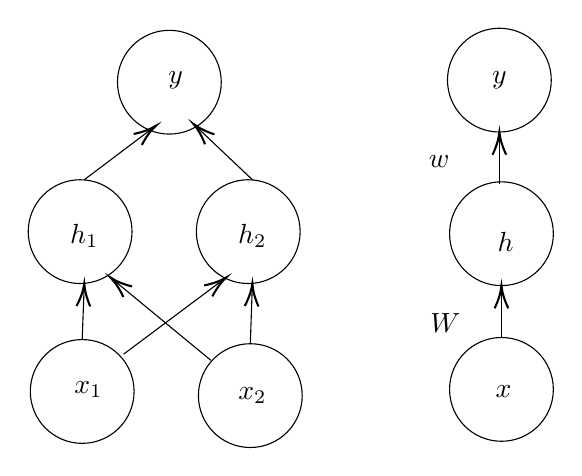
\begin{tikzpicture}[x=0.75pt,y=0.75pt,yscale=-1,xscale=1]
%uncomment if require: \path (0,311); %set diagram left start at 0, and has height of 311

%Shape: Circle [id:dp9670050296621862]
\draw   (159,99) .. controls (159,85.19) and (170.19,74) .. (184,74) .. controls (197.81,74) and (209,85.19) .. (209,99) .. controls (209,112.81) and (197.81,124) .. (184,124) .. controls (170.19,124) and (159,112.81) .. (159,99) -- cycle ;
%Shape: Circle [id:dp4168908267537763]
\draw   (116,171) .. controls (116,157.19) and (127.19,146) .. (141,146) .. controls (154.81,146) and (166,157.19) .. (166,171) .. controls (166,184.81) and (154.81,196) .. (141,196) .. controls (127.19,196) and (116,184.81) .. (116,171) -- cycle ;
%Shape: Circle [id:dp05122620984774029]
\draw   (197,171) .. controls (197,157.19) and (208.19,146) .. (222,146) .. controls (235.81,146) and (247,157.19) .. (247,171) .. controls (247,184.81) and (235.81,196) .. (222,196) .. controls (208.19,196) and (197,184.81) .. (197,171) -- cycle ;
%Shape: Circle [id:dp3775938737183049]
\draw   (117,248) .. controls (117,234.19) and (128.19,223) .. (142,223) .. controls (155.81,223) and (167,234.19) .. (167,248) .. controls (167,261.81) and (155.81,273) .. (142,273) .. controls (128.19,273) and (117,261.81) .. (117,248) -- cycle ;
%Shape: Circle [id:dp24074682910663836]
\draw   (198,250) .. controls (198,236.19) and (209.19,225) .. (223,225) .. controls (236.81,225) and (248,236.19) .. (248,250) .. controls (248,263.81) and (236.81,275) .. (223,275) .. controls (209.19,275) and (198,263.81) .. (198,250) -- cycle ;
%Shape: Circle [id:dp45197376241473264]
\draw   (318,98) .. controls (318,84.19) and (329.19,73) .. (343,73) .. controls (356.81,73) and (368,84.19) .. (368,98) .. controls (368,111.81) and (356.81,123) .. (343,123) .. controls (329.19,123) and (318,111.81) .. (318,98) -- cycle ;
%Shape: Circle [id:dp0024234701391929736]
\draw   (319,172) .. controls (319,158.19) and (330.19,147) .. (344,147) .. controls (357.81,147) and (369,158.19) .. (369,172) .. controls (369,185.81) and (357.81,197) .. (344,197) .. controls (330.19,197) and (319,185.81) .. (319,172) -- cycle ;
%Shape: Circle [id:dp2445855423211074]
\draw   (319,247) .. controls (319,233.19) and (330.19,222) .. (344,222) .. controls (357.81,222) and (369,233.19) .. (369,247) .. controls (369,260.81) and (357.81,272) .. (344,272) .. controls (330.19,272) and (319,260.81) .. (319,247) -- cycle ;
%Straight Lines [id:da8979998598096157]
\draw    (142,223) -- (142.93,198) ;
\draw [shift={(143,196)}, rotate = 452.12] [color={rgb, 255:red, 0; green, 0; blue, 0 }  ][line width=0.75]    (10.93,-3.29) .. controls (6.95,-1.4) and (3.31,-0.3) .. (0,0) .. controls (3.31,0.3) and (6.95,1.4) .. (10.93,3.29)   ;

%Straight Lines [id:da2733647310285743]
\draw    (143,146) -- (175.9,121.2) ;
\draw [shift={(177.5,120)}, rotate = 503] [color={rgb, 255:red, 0; green, 0; blue, 0 }  ][line width=0.75]    (10.93,-3.29) .. controls (6.95,-1.4) and (3.31,-0.3) .. (0,0) .. controls (3.31,0.3) and (6.95,1.4) .. (10.93,3.29)   ;

%Straight Lines [id:da2565371830117549]
\draw    (224,146) -- (196.95,120.38) ;
\draw [shift={(195.5,119)}, rotate = 403.45] [color={rgb, 255:red, 0; green, 0; blue, 0 }  ][line width=0.75]    (10.93,-3.29) .. controls (6.95,-1.4) and (3.31,-0.3) .. (0,0) .. controls (3.31,0.3) and (6.95,1.4) .. (10.93,3.29)   ;

%Straight Lines [id:da01609704104865406]
\draw    (223,225) -- (223.93,198) ;
\draw [shift={(224,196)}, rotate = 451.97] [color={rgb, 255:red, 0; green, 0; blue, 0 }  ][line width=0.75]    (10.93,-3.29) .. controls (6.95,-1.4) and (3.31,-0.3) .. (0,0) .. controls (3.31,0.3) and (6.95,1.4) .. (10.93,3.29)   ;

%Straight Lines [id:da5719660304309864]
\draw    (162,230) -- (209.9,194.2) ;
\draw [shift={(211.5,193)}, rotate = 503.22] [color={rgb, 255:red, 0; green, 0; blue, 0 }  ][line width=0.75]    (10.93,-3.29) .. controls (6.95,-1.4) and (3.31,-0.3) .. (0,0) .. controls (3.31,0.3) and (6.95,1.4) .. (10.93,3.29)   ;

%Straight Lines [id:da2960094448519832]
\draw    (204,233) -- (157.04,194.27) ;
\draw [shift={(155.5,193)}, rotate = 399.51] [color={rgb, 255:red, 0; green, 0; blue, 0 }  ][line width=0.75]    (10.93,-3.29) .. controls (6.95,-1.4) and (3.31,-0.3) .. (0,0) .. controls (3.31,0.3) and (6.95,1.4) .. (10.93,3.29)   ;

%Straight Lines [id:da3873201619155475]
\draw    (344,222) -- (344,199) ;
\draw [shift={(344,197)}, rotate = 450] [color={rgb, 255:red, 0; green, 0; blue, 0 }  ][line width=0.75]    (10.93,-3.29) .. controls (6.95,-1.4) and (3.31,-0.3) .. (0,0) .. controls (3.31,0.3) and (6.95,1.4) .. (10.93,3.29)   ;

%Straight Lines [id:da43751278888135303]
\draw    (343,148) -- (343,125) ;
\draw [shift={(343,123)}, rotate = 450] [color={rgb, 255:red, 0; green, 0; blue, 0 }  ][line width=0.75]    (10.93,-3.29) .. controls (6.95,-1.4) and (3.31,-0.3) .. (0,0) .. controls (3.31,0.3) and (6.95,1.4) .. (10.93,3.29)   ;


% Text Node
\draw (145,247) node   {$x_{1}$};
% Text Node
\draw (224,250) node   {$x_{2}$};
% Text Node
\draw (143,173) node   {$h_{1}$};
% Text Node
\draw (224,173) node   {$h_{2}$};
% Text Node
\draw (187,98) node   {$y$};
% Text Node
\draw (345,248) node   {$x$};
% Text Node
\draw (346,176) node   {$h$};
% Text Node
\draw (343,98) node   {$y$};
% Text Node
\draw (317,215) node   {$W$};
% Text Node
\draw (314,137) node   {$w$};


\end{tikzpicture}
} }%
    \qquad
    \subfloat[\acrshort{rnn}]{\resizebox{8cm}{!}{

\tikzset{every picture/.style={line width=0.75pt}} %set default line width to 0.75pt

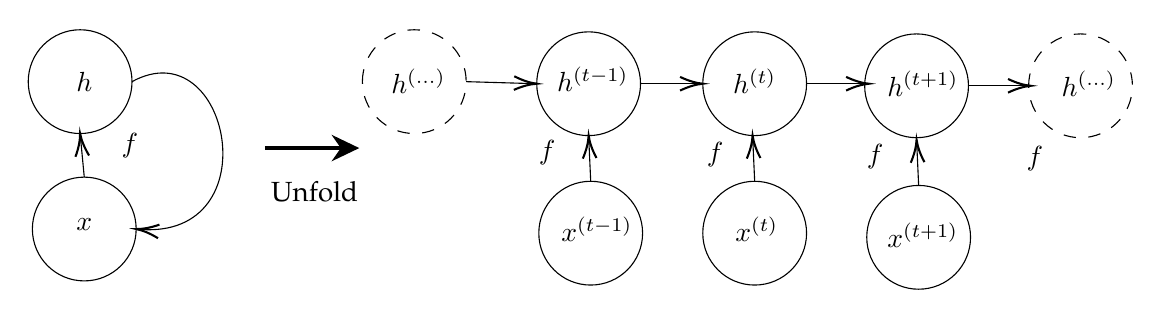
\begin{tikzpicture}[x=0.75pt,y=0.75pt,yscale=-1,xscale=1]
%uncomment if require: \path (0,226); %set diagram left start at 0, and has height of 226

%Shape: Circle [id:dp8915977439027853]
\draw   (34,95) .. controls (34,81.19) and (45.19,70) .. (59,70) .. controls (72.81,70) and (84,81.19) .. (84,95) .. controls (84,108.81) and (72.81,120) .. (59,120) .. controls (45.19,120) and (34,108.81) .. (34,95) -- cycle ;
%Shape: Circle [id:dp1742038383171982]
\draw   (36,166) .. controls (36,152.19) and (47.19,141) .. (61,141) .. controls (74.81,141) and (86,152.19) .. (86,166) .. controls (86,179.81) and (74.81,191) .. (61,191) .. controls (47.19,191) and (36,179.81) .. (36,166) -- cycle ;
%Shape: Circle [id:dp778351744563933]
\draw  [dash pattern={on 4.5pt off 4.5pt}] (195,95) .. controls (195,81.19) and (206.19,70) .. (220,70) .. controls (233.81,70) and (245,81.19) .. (245,95) .. controls (245,108.81) and (233.81,120) .. (220,120) .. controls (206.19,120) and (195,108.81) .. (195,95) -- cycle ;
%Shape: Circle [id:dp39356034990885047]
\draw   (279,96) .. controls (279,82.19) and (290.19,71) .. (304,71) .. controls (317.81,71) and (329,82.19) .. (329,96) .. controls (329,109.81) and (317.81,121) .. (304,121) .. controls (290.19,121) and (279,109.81) .. (279,96) -- cycle ;
%Shape: Circle [id:dp8163613617079115]
\draw   (359,96) .. controls (359,82.19) and (370.19,71) .. (384,71) .. controls (397.81,71) and (409,82.19) .. (409,96) .. controls (409,109.81) and (397.81,121) .. (384,121) .. controls (370.19,121) and (359,109.81) .. (359,96) -- cycle ;
%Shape: Circle [id:dp2250747213748785]
\draw   (437,97) .. controls (437,83.19) and (448.19,72) .. (462,72) .. controls (475.81,72) and (487,83.19) .. (487,97) .. controls (487,110.81) and (475.81,122) .. (462,122) .. controls (448.19,122) and (437,110.81) .. (437,97) -- cycle ;
%Shape: Circle [id:dp2879609852019731]
\draw  [dash pattern={on 4.5pt off 4.5pt}] (516,97) .. controls (516,83.19) and (527.19,72) .. (541,72) .. controls (554.81,72) and (566,83.19) .. (566,97) .. controls (566,110.81) and (554.81,122) .. (541,122) .. controls (527.19,122) and (516,110.81) .. (516,97) -- cycle ;
%Shape: Circle [id:dp6135697452809603]
\draw   (280,168) .. controls (280,154.19) and (291.19,143) .. (305,143) .. controls (318.81,143) and (330,154.19) .. (330,168) .. controls (330,181.81) and (318.81,193) .. (305,193) .. controls (291.19,193) and (280,181.81) .. (280,168) -- cycle ;
%Shape: Circle [id:dp3618767155006668]
\draw   (359,168) .. controls (359,154.19) and (370.19,143) .. (384,143) .. controls (397.81,143) and (409,154.19) .. (409,168) .. controls (409,181.81) and (397.81,193) .. (384,193) .. controls (370.19,193) and (359,181.81) .. (359,168) -- cycle ;
%Shape: Circle [id:dp6873866287842296]
\draw   (438,170) .. controls (438,156.19) and (449.19,145) .. (463,145) .. controls (476.81,145) and (488,156.19) .. (488,170) .. controls (488,183.81) and (476.81,195) .. (463,195) .. controls (449.19,195) and (438,183.81) .. (438,170) -- cycle ;
%Straight Lines [id:da683677850542731]
\draw    (61,141) -- (59.19,121.99) ;
\draw [shift={(59,120)}, rotate = 444.56] [color={rgb, 255:red, 0; green, 0; blue, 0 }  ][line width=0.75]    (10.93,-3.29) .. controls (6.95,-1.4) and (3.31,-0.3) .. (0,0) .. controls (3.31,0.3) and (6.95,1.4) .. (10.93,3.29)   ;

%Curve Lines [id:da3208902781260641]
\draw    (84,95) .. controls (131.03,69.26) and (151.1,170.93) .. (87.94,166.18) ;
\draw [shift={(86,166)}, rotate = 366.1] [color={rgb, 255:red, 0; green, 0; blue, 0 }  ][line width=0.75]    (10.93,-3.29) .. controls (6.95,-1.4) and (3.31,-0.3) .. (0,0) .. controls (3.31,0.3) and (6.95,1.4) .. (10.93,3.29)   ;

%Straight Lines [id:da791917182295558]
\draw    (245,95) -- (277,95.94) ;
\draw [shift={(279,96)}, rotate = 181.68] [color={rgb, 255:red, 0; green, 0; blue, 0 }  ][line width=0.75]    (10.93,-3.29) .. controls (6.95,-1.4) and (3.31,-0.3) .. (0,0) .. controls (3.31,0.3) and (6.95,1.4) .. (10.93,3.29)   ;

%Straight Lines [id:da9132315095017465]
\draw    (329,96) -- (357,96) ;
\draw [shift={(359,96)}, rotate = 180] [color={rgb, 255:red, 0; green, 0; blue, 0 }  ][line width=0.75]    (10.93,-3.29) .. controls (6.95,-1.4) and (3.31,-0.3) .. (0,0) .. controls (3.31,0.3) and (6.95,1.4) .. (10.93,3.29)   ;

%Straight Lines [id:da059718808747310836]
\draw    (409,96) -- (437,96) ;
\draw [shift={(439,96)}, rotate = 180] [color={rgb, 255:red, 0; green, 0; blue, 0 }  ][line width=0.75]    (10.93,-3.29) .. controls (6.95,-1.4) and (3.31,-0.3) .. (0,0) .. controls (3.31,0.3) and (6.95,1.4) .. (10.93,3.29)   ;

%Straight Lines [id:da5002222570015804]
\draw    (487,97) -- (515,97) ;
\draw [shift={(517,97)}, rotate = 180] [color={rgb, 255:red, 0; green, 0; blue, 0 }  ][line width=0.75]    (10.93,-3.29) .. controls (6.95,-1.4) and (3.31,-0.3) .. (0,0) .. controls (3.31,0.3) and (6.95,1.4) .. (10.93,3.29)   ;

%Straight Lines [id:da8281402808561851]
\draw    (305,143) -- (304.09,123) ;
\draw [shift={(304,121)}, rotate = 447.4] [color={rgb, 255:red, 0; green, 0; blue, 0 }  ][line width=0.75]    (10.93,-3.29) .. controls (6.95,-1.4) and (3.31,-0.3) .. (0,0) .. controls (3.31,0.3) and (6.95,1.4) .. (10.93,3.29)   ;

%Straight Lines [id:da010331238693556566]
\draw    (384,143) -- (383.09,123) ;
\draw [shift={(383,121)}, rotate = 447.4] [color={rgb, 255:red, 0; green, 0; blue, 0 }  ][line width=0.75]    (10.93,-3.29) .. controls (6.95,-1.4) and (3.31,-0.3) .. (0,0) .. controls (3.31,0.3) and (6.95,1.4) .. (10.93,3.29)   ;

%Straight Lines [id:da7804581287253609]
\draw    (463,145) -- (462.09,125) ;
\draw [shift={(462,123)}, rotate = 447.4] [color={rgb, 255:red, 0; green, 0; blue, 0 }  ][line width=0.75]    (10.93,-3.29) .. controls (6.95,-1.4) and (3.31,-0.3) .. (0,0) .. controls (3.31,0.3) and (6.95,1.4) .. (10.93,3.29)   ;

%Straight Lines [id:da7864502639069382]
\draw [line width=1.5]    (148,127) -- (190.5,127) ;
\draw [shift={(193.5,127)}, rotate = 180] [fill={rgb, 255:red, 0; green, 0; blue, 0 }  ][line width=1.5]  [draw opacity=0] (13.4,-6.43) -- (0,0) -- (13.4,6.44) -- (8.9,0) -- cycle    ;


% Text Node
\draw (61,164) node   {$x$};
% Text Node
\draw (83,126) node   {$f$};
% Text Node
\draw (61,95) node   {$h$};
% Text Node
\draw (222,95) node   {$h^{( ...)}$};
% Text Node
\draw (306,94) node   {$h^{( t-1)}$};
% Text Node
\draw (465,96) node   {$h^{( t+1)}$};
% Text Node
\draw (384,95) node   {$h^{( t)}$};
% Text Node
\draw (545,96) node   {$h^{( ...)}$};
% Text Node
\draw (308,166) node   {$x^{( t-1)}$};
% Text Node
\draw (465,169) node   {$x^{( t+1)}$};
% Text Node
\draw (385,166) node   {$x^{( t)}$};
% Text Node
\draw (172,148) node  [align=left] {Unfold};
% Text Node
\draw (284,129) node   {$f$};
% Text Node
\draw (365,130) node   {$f$};
% Text Node
\draw (442,131) node   {$f$};
% Text Node
\draw (519,132) node   {$f$};


\end{tikzpicture}
} }%
    \caption{A Feed Forward Network (FFN) and a Recurrent Neural Network (\acrshort{rnn})}%
    \label{fig:bg_fnn_rnn}%
  \end{figure}


\subsection{Recurrent Neural Networks and LSTMs}
\label{sec:bg_rnn_lstm}

\acrshort{rnn} employ a feedback connection by repeatedly applying FNN (Figure \ref{fig:bg_fnn_rnn}). The addition of the feedback loops to the hidden units of an MLP can be thought of forming a hidden state of the network $h(x)$, corresponding to the vector of activations (value after the non-linearity) of the hidden neurons, that evolves over time as we present inputs to the network. The hidden state is updated at each time step according to some function $f$:

\begin{equation}
    h_t = f(h_{t-1}, x_t)
\end{equation}{}

\acrshort{rnn}s are learned by computing gradients through time, which is also known as Back Propagation Through Time (BPTT) \citep{rumelhart1986learning}.

While repeatedly applying the FNNs to create an \acrshort{rnn}, the architecture faces a critical ``vanishing and exploding gradient" problem \citep{hochreiter2001gradient}, i.e., the gradients either become too insignificant or too big while backpropagating through multiple non-linear layers. To overcome this problem, Long Short-Term Memory \citep{hochreiter1997long} was proposed which consists of a specific gating architecture to overcome the problem to a great extent. The standard LSTM architecture is described in Figure \ref{fig:bg_lstm}.

\begin{figure}
  \centering
  \resizebox{10cm}{!}{

\tikzset{every picture/.style={line width=0.75pt}} %set default line width to 0.75pt

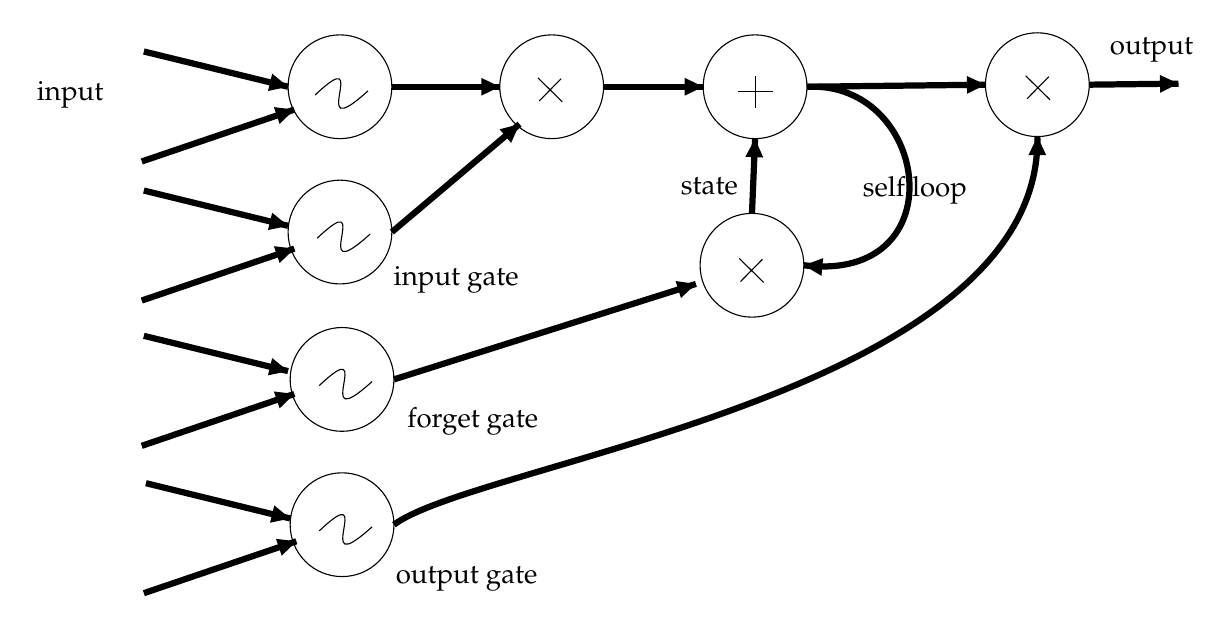
\begin{tikzpicture}[x=0.75pt,y=0.75pt,yscale=-1,xscale=1]
%uncomment if require: \path (0,377); %set diagram left start at 0, and has height of 377

\draw    (167, 81) circle [x radius= 25, y radius= 25]  ;
\draw    (167, 151) circle [x radius= 25, y radius= 25]  ;
\draw    (168, 222) circle [x radius= 25, y radius= 25]  ;
\draw    (168, 292) circle [x radius= 25, y radius= 25]  ;
\draw    (269, 81) circle [x radius= 25, y radius= 25]  ;
\draw    (367, 81) circle [x radius= 25, y radius= 25]  ;
\draw    (503, 80) circle [x radius= 25, y radius= 25]  ;
\draw [line width=2.25]    (72.5,64) -- (142,81) ;
\draw [shift={(142,81)}, rotate = 193.74] [fill={rgb, 255:red, 0; green, 0; blue, 0 }  ][line width=2.25]  [draw opacity=0] (8.93,-4.29) -- (0,0) -- (8.93,4.29) -- (8.93,-4.29)    ;

\draw [line width=2.25]    (71.5,117) -- (145,92) ;
\draw [shift={(145,92)}, rotate = 521.21] [fill={rgb, 255:red, 0; green, 0; blue, 0 }  ][line width=2.25]  [draw opacity=0] (8.93,-4.29) -- (0,0) -- (8.93,4.29) -- (8.93,-4.29)    ;

\draw [line width=2.25]    (72.5,131) -- (142,148) ;
\draw [shift={(142,148)}, rotate = 193.74] [fill={rgb, 255:red, 0; green, 0; blue, 0 }  ][line width=2.25]  [draw opacity=0] (8.93,-4.29) -- (0,0) -- (8.93,4.29) -- (8.93,-4.29)    ;

\draw [line width=2.25]    (71.5,184) -- (145,159) ;
\draw [shift={(145,159)}, rotate = 521.21] [fill={rgb, 255:red, 0; green, 0; blue, 0 }  ][line width=2.25]  [draw opacity=0] (8.93,-4.29) -- (0,0) -- (8.93,4.29) -- (8.93,-4.29)    ;

\draw [line width=2.25]    (72.5,201) -- (142,218) ;
\draw [shift={(142,218)}, rotate = 193.74] [fill={rgb, 255:red, 0; green, 0; blue, 0 }  ][line width=2.25]  [draw opacity=0] (8.93,-4.29) -- (0,0) -- (8.93,4.29) -- (8.93,-4.29)    ;

\draw [line width=2.25]    (71.5,254) -- (145,229) ;
\draw [shift={(145,229)}, rotate = 521.21] [fill={rgb, 255:red, 0; green, 0; blue, 0 }  ][line width=2.25]  [draw opacity=0] (8.93,-4.29) -- (0,0) -- (8.93,4.29) -- (8.93,-4.29)    ;

\draw [line width=2.25]    (73.5,272) -- (143,289) ;
\draw [shift={(143,289)}, rotate = 193.74] [fill={rgb, 255:red, 0; green, 0; blue, 0 }  ][line width=2.25]  [draw opacity=0] (8.93,-4.29) -- (0,0) -- (8.93,4.29) -- (8.93,-4.29)    ;

\draw [line width=2.25]    (72.5,325) -- (146,300) ;
\draw [shift={(146,300)}, rotate = 521.21] [fill={rgb, 255:red, 0; green, 0; blue, 0 }  ][line width=2.25]  [draw opacity=0] (8.93,-4.29) -- (0,0) -- (8.93,4.29) -- (8.93,-4.29)    ;

\draw [line width=2.25]    (192,81) -- (244,81) ;
\draw [shift={(244,81)}, rotate = 180] [fill={rgb, 255:red, 0; green, 0; blue, 0 }  ][line width=2.25]  [draw opacity=0] (8.93,-4.29) -- (0,0) -- (8.93,4.29) -- (8.93,-4.29)    ;

\draw [line width=2.25]    (192,151) -- (253.5,99) ;
\draw [shift={(253.5,99)}, rotate = 499.78] [fill={rgb, 255:red, 0; green, 0; blue, 0 }  ][line width=2.25]  [draw opacity=0] (8.93,-4.29) -- (0,0) -- (8.93,4.29) -- (8.93,-4.29)    ;

\draw    (365.5, 167) circle [x radius= 25, y radius= 25]  ;
\draw [line width=2.25]    (193,222) -- (338.5,176) ;
\draw [shift={(338.5,176)}, rotate = 522.46] [fill={rgb, 255:red, 0; green, 0; blue, 0 }  ][line width=2.25]  [draw opacity=0] (8.93,-4.29) -- (0,0) -- (8.93,4.29) -- (8.93,-4.29)    ;

\draw [line width=2.25]    (365.5,142) -- (367,106) ;
\draw [shift={(367,106)}, rotate = 452.39] [fill={rgb, 255:red, 0; green, 0; blue, 0 }  ][line width=2.25]  [draw opacity=0] (8.93,-4.29) -- (0,0) -- (8.93,4.29) -- (8.93,-4.29)    ;

\draw [line width=2.25]    (392,81) .. controls (451.5,78) and (464.5,176) .. (390.5,167) ;
\draw [shift={(390.5,167)}, rotate = 365.44] [fill={rgb, 255:red, 0; green, 0; blue, 0 }  ][line width=2.25]  [draw opacity=0] (8.93,-4.29) -- (0,0) -- (8.93,4.29) -- (8.93,-4.29)    ;

\draw [line width=2.25]    (294,81) -- (342,81) ;
\draw [shift={(342,81)}, rotate = 180] [fill={rgb, 255:red, 0; green, 0; blue, 0 }  ][line width=2.25]  [draw opacity=0] (8.93,-4.29) -- (0,0) -- (8.93,4.29) -- (8.93,-4.29)    ;

\draw [line width=2.25]    (392,81) -- (478,80) ;
\draw [shift={(478,80)}, rotate = 539.3299999999999] [fill={rgb, 255:red, 0; green, 0; blue, 0 }  ][line width=2.25]  [draw opacity=0] (8.93,-4.29) -- (0,0) -- (8.93,4.29) -- (8.93,-4.29)    ;

\draw [line width=2.25]    (528,80) -- (571,79.5) ;
\draw [shift={(571,79.5)}, rotate = 539.3299999999999] [fill={rgb, 255:red, 0; green, 0; blue, 0 }  ][line width=2.25]  [draw opacity=0] (8.93,-4.29) -- (0,0) -- (8.93,4.29) -- (8.93,-4.29)    ;

\draw [line width=2.25]    (193,292) .. controls (233,262) and (505.5,229) .. (503,105) ;
\draw [shift={(503,105)}, rotate = 450.11] [fill={rgb, 255:red, 0; green, 0; blue, 0 }  ][line width=2.25]  [draw opacity=0] (8.93,-4.29) -- (0,0) -- (8.93,4.29) -- (8.93,-4.29)    ;

\draw    (155,85) .. controls (183.5,58) and (149.5,111) .. (180.5,83) ;


\draw    (156,154) .. controls (184.5,127) and (150.5,180) .. (181.5,152) ;


\draw    (157,225) .. controls (185.5,198) and (151.5,251) .. (182.5,223) ;


\draw    (157,295) .. controls (185.5,268) and (151.5,321) .. (182.5,293) ;


\draw   (359,83.5) -- (375.5,83.5)(367.25,76) -- (367.25,91) ;
\draw [rotate around= { 44.59: (365.25, 169.5)
    }]  (357,169.5) -- (373.5,169.5)(365.25,162) -- (365.25,177) ;
\draw [rotate around= { 44.59: (268.25, 82.5)
    }]  (260,82.5) -- (276.5,82.5)(268.25,75) -- (268.25,90) ;
\draw [rotate around= { 44.59: (503.25, 81.5)
    }]  (495,81.5) -- (511.5,81.5)(503.25,74) -- (503.25,89) ;

\draw (558,63) node  [align=left] {output};
\draw (37,85) node  [align=left] {input};
\draw (223,174) node  [align=left] {input gate};
\draw (231,242) node  [align=left] {forget gate};
\draw (228,318) node  [align=left] {output gate};
\draw (345,129) node  [align=left] {state};
\draw (444,131) node  [align=left] {self loop};


\end{tikzpicture}
}
  \caption{Block diagram of LSTM cell.}
  \label{fig:bg_lstm}
\end{figure}

Given an input sequence, LSTM can also be run in both directions to get two final representations $\overrightarrow{y_t}$ in the forward direction and $\overleftarrow{y_t}$ in the backward direction. This class of modified LSTM is known as Bidirectional LSTM and it has been used as a standard feature extractor in various natural language processing tasks \cite{Rocktaschel2015-rr, wang2016machine, serban2016building}. In language modelling \& machine translation tasks \citep{serban2016building, serban2017hierarchical, bahdanau2014neural}, BiLSTM is used to construct an \textit{encoded} representation of the input text, conditioned on which the next word in the output text is \textit{decoded}. For textual entailment tasks \citep{bowman-etal-2015-large}, two individual sentence representations of the hypothesis and premise are calculated using BiLSTM, and the entailment is predicted over the concatenated representation \citep{Rocktaschel2015-rr}. For QA tasks, the natural language question is encoded through a BiLSTM and the sentence representation is used in downstream reasoning \citep{wang2016machine}. Given the gated memory structure of LSTM and bidirectional read, they provide a powerful mechanism to convert text into a fixed vector representation which captures various syntactic and semantic features of natural language \citep{conneau2018cram}.


\subsection{Transformer Models}
\label{sec:bg_transformers}

In contrast to \acrshort{rnn}s and LSTMs, Transformer \citep{vaswani-etal-2017-attention} architectures eliminate the need of recurrent connections and instead use fully connected self-attention layers. Attention mechanisms \citep{bahdanau2014neural} were previously developed to improve \acrshort{rnn}s and LSTMs to allow the model to condition on longer contexts than what the default recurrence provides. Transformer architecture leverages this attention mechanism to attend on the same input (hence the name ``self-attention'') in multiple layers, this allowing the model to bypass the need of recurrence and directly utilize the information from any context.

\subsubsection{Self-attention}

Transformer architecture maps an input sequence ($x_{1}, x_{2}, \ldots, x_{n}$) to an output sequence ($y_{1}, y_{2}, \ldots, y_{n}$) of the same length, hence being a transductive model. Self-attention consists of computing vector similarities, using the dot product, between a pair of inputs:

\begin{equation}
  \text{score}(x_{i},x_{j}) = x_{i}.x_{j}
\end{equation}

This dot product yields scalar values in $\mathbb{R}$. Attention from each input to any other input is computed as the softmax over the dot product value in order to capture the proportional probability of similarity between tokens. This attention value is then multiplied by the inputs to compute the output at a sequence element. Every input is restricted to attend to all inputs beyond its position, thereby mimicing the canonical language modeling setup (although Markov assumptions no longer hold here due to the linear combination).

\begin{equation}
  \alpha_{i,j} = \frac{\text{exp}(\text{score}(x_{i},x_{j}))}{\sum_{k=1}^{i}\text{exp}(\text{score}(x_{i},x_{k}))}
\end{equation}

\begin{equation}
  y_{i} = \sum_{j \le i}\alpha_{i,j}x_{j}
\end{equation}

Using this basic formulation, Transformers first map the inputs into three distinct vectors, \textit{query} ($q$), \textit{key} ($k$) and \textit{value} ($v$). When computing the attention from the current input to a preceding input, the model chooses to compute the score between the query mapping of the current input against the key mapping of the preceding input. This score is then using to linearly combine the value mappings of preceding inputs to compute the output for the current token. In practice, this score can become unbounded and lead to numerical issues. Therefore, the score is normalized by dividing with the square root of the dimensionality of the query and key vectors.

\begin{equation}
  q_{i} = \theta_{q}x_{i}, k_{i} = \theta_{k}x_{i}, v_{i} = \theta_{v}x_{i}
\end{equation}

\begin{equation}
  \text{score}(x_{i},x_{j}) = \frac{q_{i}.k_{j}}{\sqrt{d_{k}}}
\end{equation}

\begin{equation}
  y_{i} = \sum_{j \le i}\alpha_{i,j}v_{j}
\end{equation}

This attention mechanism is now stacked in two dimensions. First, the same attention mechanism is applied multiple times using unique set of weights. This is known as \textit{multi-head} attention, to emulate multiple heads (or weights) being utilized to compute unique sets of attentions for the same current and preceding input pair. The resulting attention mechanism is referred to as an \textit{attention-layer}.
Second, the attention layers can be stacked on top of each other to emulate a multi-layer neural network. Typically, a feed-forward layer, layer normalizations \citep{ba2016layer} and residual connections are applied after one attention layer to convert it to a \textit{transformer block}, which is then stacked vertically in multiple layers (\autoref{fig:bg_transformer}).

\begin{figure}
  \centering
  \resizebox{0.4\textwidth}{!}{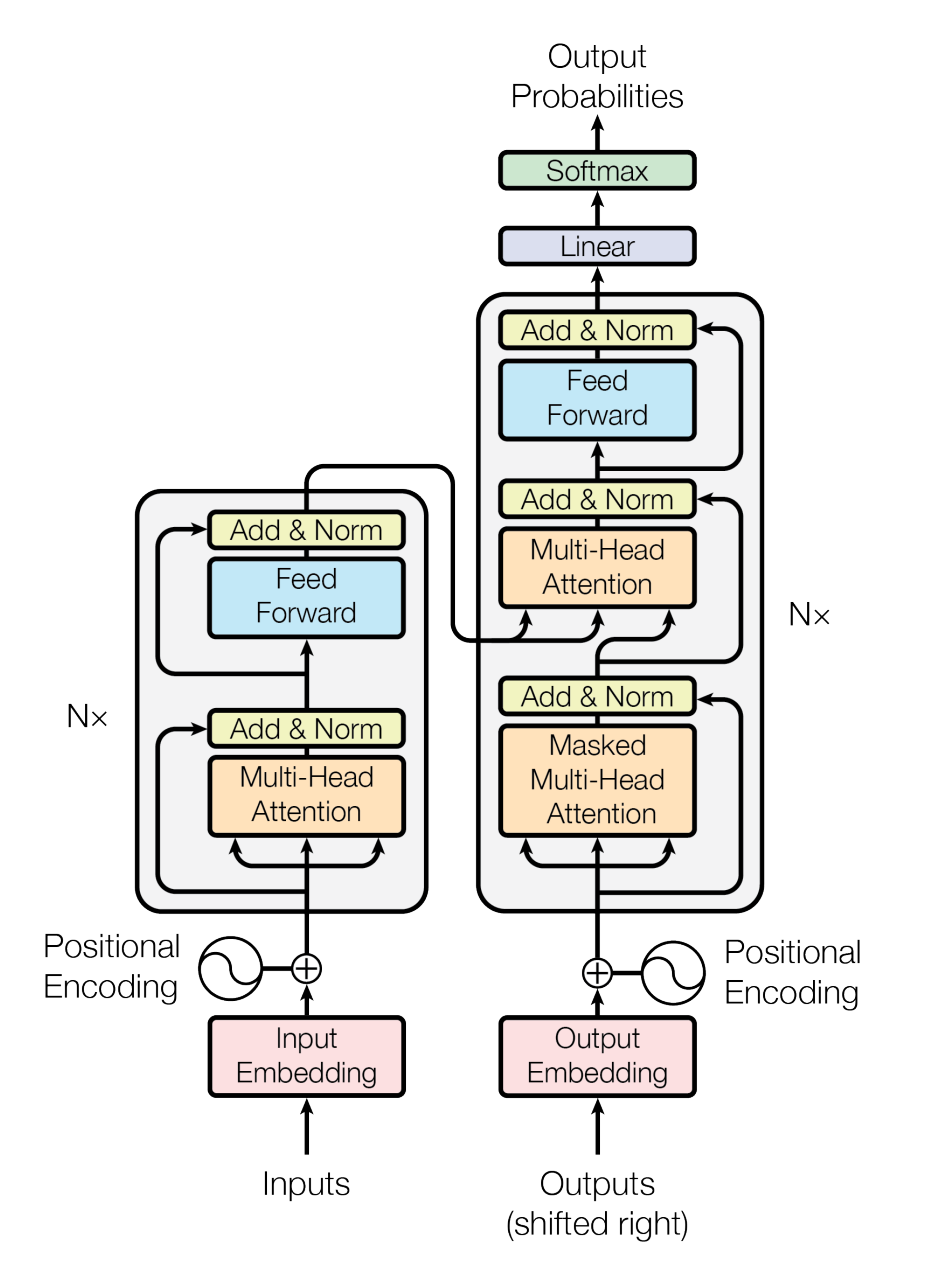
\includegraphics{figs/background/transformer_arch.png}}
  \caption{Transformer encoder block as described in \citet{vaswani-etal-2017-attention}.}
  \label{fig:bg_transformer}
\end{figure}

\subsubsection{Position embeddings}
\label{sec:bg_position_embeddings}

One drawback of the vanilla Transformer architecture is that word order cannot be represented, as due to linear combination of attention scores the individual inputs can be re-arranged to get the exact same output. Thus, position information is fed to the model by representing the position of each token using a feature vector. \citet{vaswani-etal-2017-attention} use absolute word position information as a feature vector, which is derived from an alternating sine and cosine functions:

\begin{equation}
  \begin{aligned}
	\text{PE}(pos, 2i) &= \text{sin}(pos / 10000^{2i / d}) \\
    \text{PE}(pos, 2i+1) &= \text{cos}(pos / 10000^{2i / d})
  \end{aligned}
\end{equation}

\noindent $\text{PE}$ is the position embedding matrix of size $m \times d$, where $m$ is the total number of positions supported by the model, and $d$ is the dimensionality of the positional embedding. $d$ is kept as same as the embedding dimensionality of the input $x_{i}$ such that the input representation is updated with the positional features by element-wise sum \textit{before} applying the self-attention mechanism.

\begin{equation}
  x_{i} = x_{i} + \text{PE}[i]
\end{equation}

Subsequently, a unique learned position feature is used to define the absolute position encoding \citep{devlin-etal-2019-bert}. Instead of using a fixed function, the model can use a learned positional matrix $\theta_{PE} \in \mathcal{R}^{m \times d}$ of the same dimension (commonly referred to as learned positional embedding), where the features are learned by backpropagation during training.

While absolute position encodings, especially learned position embeddings are still used by many variants of the Transformer models, it lacks the capacity to model relative position distances between tokens \footnote{In Chapter \ref{sec:pos}, we investigate in detail several shortcomings of the learned position embedding scheme}. Thus, relative positional encodings were proposed \citep{shaw-etal-2018-self} which directly encode the relative distance between the words. Specifically, instead of maintaining a large embedding matrix ($\theta_{PE}$), a smaller embedding matrix is now maintained based on a window size $r$, and dynamically compute the position encoding of a token based on the relative distances between the current token and its neighbors within the window of size $r$.
Please refer to \citet{wang2021on,dufter2021position} for a comprehensive overview of different position encoding strategies.

\subsection{Pre-training and the advent of large language models}
\label{sec:bg_pretraining}

Transformer architectures introduce mechanisms to drastically increase the amount of trainable model parameters, compared to \acrshort{rnn} and LSTM counterparts.
With increasing number of model parameters, the requirement to train on large datasets became inevitable - as otherwise it is not possible to fully train the model parameters. However, it is challenging to design tasks of such scale due to extremely expensive annotation costs. In contrast, it is relatively easy to obtain large-scale unlabeled corpora, typically through scraping the internet \cite{Raffel2020:T5} or collecting all literary works \cite{zhu2015aligning}. Thus emerged the idea of \textit{pre-training} \citep{mikolov2013efficient, peters-etal-2018-deep}, where a massive, unlabeled corpus is leveraged to train a \textit{language model}, i.e. predicting the probability of tokens given the context (\autoref{sec:bg_ngram_lang}). Given an input context, the aim of a given model is to compute a representation of the same, in order to predict the next token probability distribution, typically in the form of a softmax function over the full vocabulary. Learning such a language model on top of the massive corpora yields better contextual token representation, which are then utilized to perform various downstream tasks. The large, unlabeled data can be leveraged to learn useful word embeddings either using pairwise ranking \citep{collobert2008unified}, or through the use of shallow architectures \citep{mikolov2013efficient}, or by computing global word-word co-occurence statistics \citep{pennington2014glove}. However, these pre-trained word embeddings are still context-independent, and requires learning context-dependent parameters from scratch on the downstream task. Thus, efforts have been made to pre-train the entire model parameters instead of generating word embeddings by training in a language modeling objective, using bidirectional LSTM based architectures \citep{peters-etal-2018-deep}. These models are then used to fine-tune on downstream tasks such as text classification \citep{howard2018universal}.

More recently, Transformer-based architectures became widely popular with the introduction of BERT \citep{devlin-etal-2019-bert}. BERT is fundamentally a stack of Transformer layers, having multiple self-attention heads. To learn its massive amount of parameters, BERT is pre-trained on unlabeled corpora using two self-supervised training objectives: masked language modeling (\acrshort{mlm}) and next sentence prediction (NSP) (predicting if two sentences are adjacent to each other). In \acrshort{mlm}, an input sentence is corrupted by randomly masking some percentage of tokens, and the objective of the model is to leverage the context to predict the correct masked tokens. In NSP, BERT is provided an additional objective to predict if two given sentences are neighbors \footnote{In the followup works, such as RoBERTa, the NSP objective has been subsequently discarded in favor of pure \acrshort{mlm} objective on larger batch sizes.}. BERT significantly improved the state-of-the art in many downstream tasks - ranging from text classication, question answering, natural language inference, machine translation, summarizatio, to name a few. Subsequently, several flavor of Transformer models have been proposed, which can be broadly classified into three distinct classes:

\begin{itemize}
  \item \textbf{Encoder-only models} This model family only consists of a $n$ layered Transformer model as the encoder, such as BERT \citep{devlin-etal-2019-bert}. This class of models is utilized to extract generalized representations of sentences, which can be further used in downstream tasks. RoBERTa \citep{liu-et-al-2019-roberta}, DistilBERT \citep{sanh2020distilbert}, ALBERT \citep{lan2019albert}, ELECTRA \citep{clark2020electra} are other examples of this class of model.
  \item \textbf{Encoder-Decoder models} This is a two-step model, which was originally defined in \cite{vaswani-etal-2017-attention}. The model architecture contains two separate stacked Transformer layers, where the first stack is used to \textit{encode} the sentence representation, and the second stack is used to generate the target text conditioned on the encoded representation (i.e., to \textit{decode}). BART \citep{lewis-etal-2020-bart}, mBART \citep{liu2020multilingual}, T5 \citep{Raffel2020:T5} are more examples of this class of models.
  \item \textbf{Decoder-only models} In this family of models, they consist of only the decoder element to predict the text from a given input, without having a dedicated encoder block. The goal of these models if the predict the next token given a sentence or paragraph. GPT2 \citep{Radford2019:GPT2}, GPT-3 \citep{Brown2020:GPT3}, Transformer-XL \cite{dai-etal-2019-transformer} are models of this type.
\end{itemize}

Transformer models can also be classified based on the type of training objective used while pre-training. Broadly, they can be grouped into two classes:

\begin{itemize}
  \item \textbf{Masked Language Models} Popularized by BERT \citep{devlin-etal-2019-bert}, this family of models in its core uses the technique of predicting the masked tokens in a given corrupted input. Thus, these type of models are typically \textit{bidirectional}, as in they have the ability to leverage contextual information in the input sentence from both directions. RoBERTa, BART, ALBERT, ELECTRA etc are examples of this class of Transformer models.
  \item \textbf{Autoregressive Language Models} On the other hand, the vanilla Transformer model was proposed as an autoregressive model, where the model does not have the contextual information from both directions of the input. These models mimic the classical language model setup (\autoref{sec:bg_ngram_lang}), where given a sequence of tokens the model only uses the previously seen tokens as context to generate the next set of tokens, hence they are also known as \textit{uni-directional} models. GPT-2, GPT-3, T5, Transformer-XL are examples of this class of Transformer models.
\end{itemize}

\section{Evaluation of text representation capacity}

\subsection{Standard tasks for measuring progress in \acrshort{nlu}}

With the advent of better and higher capacity models to represent text, the need for evaluating the progress in natural language understanding (\acrshort{nlu}) gave rise to development of various tasks and datasets. Popular instances of the datasets include SQUAD \citep{rajpurkar-etal-2016-squad} for Question Answering; SNLI \citep{bowman-etal-2015-large} and MNLI \citep{williams-etal-2018-broad} for Natural Language Inference; DecaNLP \citep{mccann2018natural} and the venerable GLUE \citep{wang-etal-2018-glue} and SuperGLUE \citep{wang-etal-2019-superglue} benchmarks for general language understanding. The GLUE benchmark was proposed to unify the measurement of progress in language understanding by using a collection of publicly released datasets:

\begin{itemize}
  \item Corpus of Linguistic Acceptability \citep[CoLA,][]{warstadt-etal-2019-neural}
  \item Stanford Sentiment Treebank \citep[SST,][]{sst2_socher2013recursive}
  \item  Microsoft Research Paragraph Corpus \citep[MRPC,][]{mrpc_dolan2005automatically}
  \item Quora Question Pairs (QQP)\footnote{\href{http://data.quora.com/First-Quora-Dataset-Release-Question-Pairs}{http://data.quora.com/First-Quora-Dataset-Release-Question-Pairs}}
  \item Multi-Genre Natural Language Inference \citep[MNLI,][]{williams-etal-2018-broad}
  \item Question NLI \citep[QNLI,][]{rajpurkar-etal-2016-squad, qnli_2_demszky2018transforming}
  \item Recognizing Textual Entailment \citep[RTE,][]{Dagan2005:RTE, rte2_haim2006second, rte3_giampiccolo2007third, rte5_bentivogli2009fifth}
  \item NLI formulation of the Winograd Schema Challenge \citep[WNLI,][]{Levesque2011:WSC}.
\end{itemize}

\noindent The SuperGLUE benchmark \citep{wang-etal-2019-superglue} was proposed following the success of GLUE as a much harder benchmark. This benchmark consist of the following datasets:

\begin{itemize}
  \item Boolean Questions \citep[BoolQ,][]{clark-etal-2019-boolq}
  \item Commitment Bank \citep[CB,][]{de2019commitmentbank}
  \item Choice of Plausible Alternatives \citep[COPA,][]{roemmele2011choice}
  \item Multi-Sentence Reading Comprehension \citep[MultiRC,][]{khashabi-etal-2018-looking}
  \item Reading Comprehension with Commonsense Reasoning Dataset \citep[ReCoRD,][]{zhang2018record}
  \item Recognizing Textual Entailment \citep[RTE,][]{Dagan2005:RTE, rte2_haim2006second, rte3_giampiccolo2007third, rte5_bentivogli2009fifth}
  \item Word-in-Context \citep[WiC,][]{pilehvar-camacho-collados-2019-wic}
  \item Winograd Schema Challenge \citep[WSC,][]{Levesque2011:WSC}
\end{itemize}

Using these benchmarks, text understanding systems have been compared against each other to measure progress in the field. While \acrshort{rnn}s and LSTMs exhibited modest performance in these tasks, the advent of attention mechanisms \citep{bahdanau2014neural} increased the performance to considerable extent. However, we witnessed meteoric improvements on these benchmarks with every release of a new variant of the Transformer model, which typically consists of increasingly large amount of parameters and have been progressively trained on greater amount of unlabeled data \citep{kaplan2020scaling}. The performance rise has even skyrocketed beyond human performance on these tasks \citep[Figure~1]{kiela-etal-2021-dynabench}. This stunning progress with the pre-trained Transformer family of models on \acrshort{nlu} taks have attracted greater investments in pre-training even larger models \citep{Brown2020:GPT3, Zhang2022:OPT}; invited researchers to dig deep into the reasoning process employed by these models \citep{rogers-etal-2020-primer}; and have invited a higher level of scrutiny of the model outputs \citep{jia-liang-2017-adversarial, gururangan-etal-2018-annotation}.

\subsection{Analysis and Interpretability}

The sheer performance of pre-trained Transformer-based models following BERT created a watershed moment in \acrshort{nlu}, as these models outperform previous LSTM-based models by a large extent, even surpassing human performance. Due to this success, interest peaked in the community to investigate the inner workings of this largely black box model \citep{rogers-etal-2020-primer}. The investigation is primarily done using the tool of \textit{probing}, which consists of learning a function on top of pre-trained representations to perform targeted assesment of linguistic information \citep{hupkes2018visualisation}. How well this probe learns a given signal can be seen as a proxy for linguistic knowledge encoded in the representations. Using these probes, it has been shown BERT representations contain adequate syntactic \citep{hewitt-manning-2019-structural,jawahar-etal-2019-bert}, semantic \citep{tenney-etal-2019-bert,ettinger-2020-whatbertisnot}, and world knowledge \citep{petroni-etal-2019-language, rogers-etal-2020-primer}.

\subsection{Brittleness issues in \acrshort{nlu} models}

Despite the large performance gain and representations containing the necessary linguistic information to process natural language, state-of-the-art \acrshort{nlu} models are often subject to scrutiny due to their unsystematic behaviors on specifically crafted test suites. \acrshort{nlu} models are repeatedly shown to be brittle when subject to adversarial attacks \cite{jia-liang-2017-adversarial,ettinger-etal-2017-towards, ettinger-2020-whatbertisnot} to the input sentence forms \cite{kaushik2018much}. \acrshort{nlu} models tend to exploit the statistical irregularities and annotation artefacts \cite{gururangan-etal-2018-annotation,poliak-etal-2018-hypothesis,tsuchiya-2018-performance} of a given datasets, resulting in failure cases on carefully crafted examples \cite{naik-etal-2018-stress,mccoy2019}.
\acrshort{nlu} models are also subjected to tests of systematic generalization in context of semantic parsing in novel compositions \cite{Lake2018:SCAN}, shuffled argument structure in natural language inference \cite{dasgupta-etal-2018-evaluating}, etc. On these tests, typically the \acrshort{nlu} models fail to behave in the expected ways, unless trained with the same objective as the test sets.

\subsection{The need for better, challenging benchmarks}

How well have our best, state-of-the-art models have progressed in \textit{human-level} language representation? We get a conflicting answer on the question. On one hand, we witness an ever increasing performance improvement on standard tasks with larger amount of parameters and longer pre-training with more data. On the other hand, we witness a stream of results showcasing the brittleness and inconsistencies of the model outputs, so much so that they fail on real world examples, unlike humans. Thus, attempts have been made to develop better benchmarks, such as Dynabench \citep{kiela-etal-2021-dynabench}. In Dynabench, models are constantly evaluated in a loop where human annotators are tasked to find harder examples to elicit an undesirable result. Dynabench is a great step in the right direction, however it poses some caveats: continuous data collection from annotators is an expensive endeavour, and the challenge nature of data collection could lead to unnatural distribution shifts \citep[Section~4, pp. 7]{kiela-etal-2021-dynabench}. The community has also invested in building newer dataset benchmarks, and have progressed to measuring zero-shot and few-shot \textit{in-context} learning evaluations to pose a significant challenge to the model. However, by nature the Transformer language models require pre-training on massive corpora, which could possibly lead to high distribution overlap between the model representation and the test dataset, resulting in memorization effects on the datasets constructed from public corpus \citep{carlini2021, carlini2022a}. Thus, we need a better mechanisms and datasets to measure the real progress of text understanding using neural models.

\section{Measuring language understanding progress using Systematicity}
\label{sec:bg_systematicity}

An alternative to measuring \textit{human-level} language understanding progress is by employing the notions of \textit{systematicity} in designing datasets and experiments.
The term is first introduced by \citet{fodor1988connectionism}, which is defined as \textit{``the ability to produce/understand some sentences is intrinsically connected to the ability to produce/understand certain others''}. This definition comes with varying interpretations in the literature \citep{Lake2018:SCAN,bahdanau2018systematic, goodwin-etal-2020-probing} and is heavily debated based on its interpretation \citep{szabo2012case,herbelot2020how}. Systematicity is also closely tied to the concept of \textit{compositionality}, which requires models to have the ability to compose and combine distinct functions to construct meaning representation \citep{kratzer1998semantics,szabo2012case}. Another term synonymous to systematicity in context is \textit{productivity}, which construes the ability of a model to generate infinite combinations of known constituents \citep{pullum2010recursion}.
For the purposes of this thesis, systematicity can be formulated into two categories:

\begin{itemize}
  \item The ability of the model to understand the \textit{recombination} of known parts and rules. In the classic example, a learner understanding the phrase ``brown dog'' and ``black cat'' also understands ``brown cat'' \citep{hupkes2020}.
  \item The ability of the model to extract \textit{consistent} contributions from words. For example, a learner understanding the phrase ``John loves Mary'' must also understand the contributions of the words ``Mary loves John'' \citep{goodwin-etal-2020-probing}.
\end{itemize}

It is heavily debated in the literature whether \textit{connectionist} architectures, such as the neural models, could account for the notions of systematicity \citep{fodor1988connectionism, smolensky1991constituent, marcus1998rethinking}. Nevertheless, the above definition of systematicity allows us to evaluate the \textit{human-ness} of the language understanding models. Systematic models employ the notions of compositionality in their representations to understand the contributions of words in the given text. Thus, a model following the principles of systematicity should exhibit the following properties:

\begin{itemize}
  \item A systematic model should be generalizable to out-of-distribution examples: any out-of-distribution example can be decomposed into known rules of syntax and meaning.
  \item It should be robust to outliers and adversarial inputs: any adversarial input will not conform with the application of known rules and thus can allow the model to circumvent processing on those inputs.
  \item It should be consistent in its understanding of words: if the rules required to understand a phrase is learned then they should yield consistent representations of the same phrase (or vice-versa, if the rule is not learned then a systematic model should not yield any useful representation for the given input).
\end{itemize}

In this thesis, we utilize the above principles of systematicity to evaluate the limits of natural language understanding of state-of-the-art \acrshort{nlu} models.

\clearpage

\chapter{Understanding semantic generalization through systematicity}
\label{chap:clutrr}

\gls{nlu} systems have been extremely successful at reading comprehension tasks, such as question answering (QA) and natural language inference (NLI).
These tasks typically test for semantic generalization, where a model has to understand the meaning of the input sentence / passage in order to perform the given task.
An array of existing datasets are available for these tasks. This includes datasets that test a system's ability to extract factual answers from text \citep{rajpurkar-etal-2016-squad,Nguyen2016-ec,Trischler2016-fc,Mostafazadeh2016-hu,Su2016-so}, as well as datasets that emphasize commonsense inference, such as entailment between sentences \citep{bowman-etal-2015-large,williams-etal-2018-broad}.

However, there are growing concerns regarding the ability of \acrshort{nlu} systems---and neural networks more generally---to generalize in a systematic and robust way \citep{bahdanau2018systematic,Lake2018:SCAN,Johnson2016-mw}.
For instance, recent work has highlighted the brittleness of \acrshort{nlu} systems to adversarial examples \citep{jia-liang-2017-adversarial}, as well as the fact that \acrshort{nlu} models tend to exploit statistical artifacts in datasets, rather than exhibiting true reasoning and generalization capabilities \citep{gururangan-etal-2018-annotation,kaushik2018much}.
These findings have also dovetailed with the recent dominance of large pre-trained language models, such as BERT, on \acrshort{nlu} benchmarks \citep{devlin-etal-2019-bert,peters-etal-2018-deep}, which suggest that the primary difficulty in these datasets is incorporating the statistics of the natural language, rather than reasoning.

An important challenge is thus to develop \acrshort{nlu} benchmarks that can precisely test a model's capability for robust and systematic generalization.
Ideally, we want language understanding systems that can not only answer questions and draw inferences from text, but that can also do so in a systematic, logical, and robust way.
While such reasoning capabilities are certainly required for many existing \acrshort{nlu} tasks, most datasets combine several challenges of language understanding into one, such as co-reference/entity resolution, incorporating world knowledge, and semantic parsing---making it difficult to isolate and diagnose a model's capabilities for systematic generalization and robustness.

In this work, we propose to use the properties of \textit{systematicity} to test the limits of semantic generalization of modern neural networks (\autoref{sec:bg_systematicity}). As defined by \citet{fodor1988connectionism}, systematicity test the ability of a system to understand the recombination of known parts and rules. Thus, inspired by the classic AI challenge of inductive logic programming \citep{Quinlan1990-iv}, in this chapter I discuss my work on developing semi-synthetic benchmark designed to explicitly test an \acrshort{nlu} model's ability for systematic and robust logical generalization \citep{sinha-etal-2019-clutrr}.
Our benchmark suite---termed \textbf{CLUTRR} (Compositional Language Understanding and Text-based Relational Reasoning)---contains a large set of semi-synthetic stories involving hypothetical families.
Given a story, the goal is to infer the relationship between two family members, whose relationship is not explicitly mentioned.
To solve this task, a learning agent must extract the relationships mentioned in the text, induce the logical rules governing the kinship relationships (e.g., the transitivity of the sibling relation), and use a combination of these rules to infer the relationship between a given pair of entities.
Crucially, the CLUTRR benchmark allows us to test a learning agent's ability for \emph{systematic generalization} by testing on stories that contain unseen combinations of logical rules.
CLUTRR also allows us to precisely test for the various forms of \emph{model robustness} by adding different kinds of superfluous \emph{noise facts} to the stories.


\section{Technical Background}
\label{sec:clutrr_bg}

\subsection{Notations and Terminology}

Following standard practice in formal semantics, we use the term \textit{atom} to refer to a \textit{predicate} symbol and a list of terms, such as $[\texttt{grandfatherOf},X,Y]$, where the predicate $\texttt{grandfatherOf}$ denotes the \textit{relation} between the two \textit{variables}, $X$ and $Y$. We restrict the predicates to have an arity of 2, i.e.,  binary predicates.
A logical \textit{rule} in this setting is of the form $\mathcal{H} \vdash \mathcal{B}$, where $\mathcal{B}$ is the \textit{body} of the rule, i.e., a conjunction of two \textit{atoms} ($[\alpha_1,\alpha_2]$) and $\mathcal{H}$ is the \textit{head}, i.e., a single \text{atom} ($\alpha$) that can be viewed as the goal or query.
For instance, given a knowledge base (KB) $R$ that contains the single rule

\begin{equation}
  [\texttt{grandfatherOf},X,Y] \vdash [[\texttt{fatherOf},X,Z], [\texttt{fatherOf}, Z,Y]],
\end{equation}

\noindent the query $[\texttt{grandfatherOf},X,Y]$ evaluates to true if and only if the body

\begin{equation}
\mathcal{B}=[[\texttt{fatherOf},X,Z], [\texttt{fatherOf}, Z,Y]]
\end{equation}

\noindent is also true in a given world.
A rule is called a \textit{grounded} rule if all atoms in the rule are themselves \textit{grounded}, i.e., all variables are replaced with \textit{constants} or entities in a world. A \textit{fact} is a grounded binary predicate. A \textit{clause} is a conjunction of two or more atoms ($\mathcal{C}=(\mathcal{H}_{\mathcal{C}} \vdash \mathcal{B}_{\mathcal{C}} = ([\alpha_1,...,\alpha_n]))$) which can be built using a set of rules.

\section{Overview and construction of CLUTRR}
\label{sec:orgf6fb520}

\begin{figure}[t]
\centering
\resizebox{0.5\textwidth}{!}{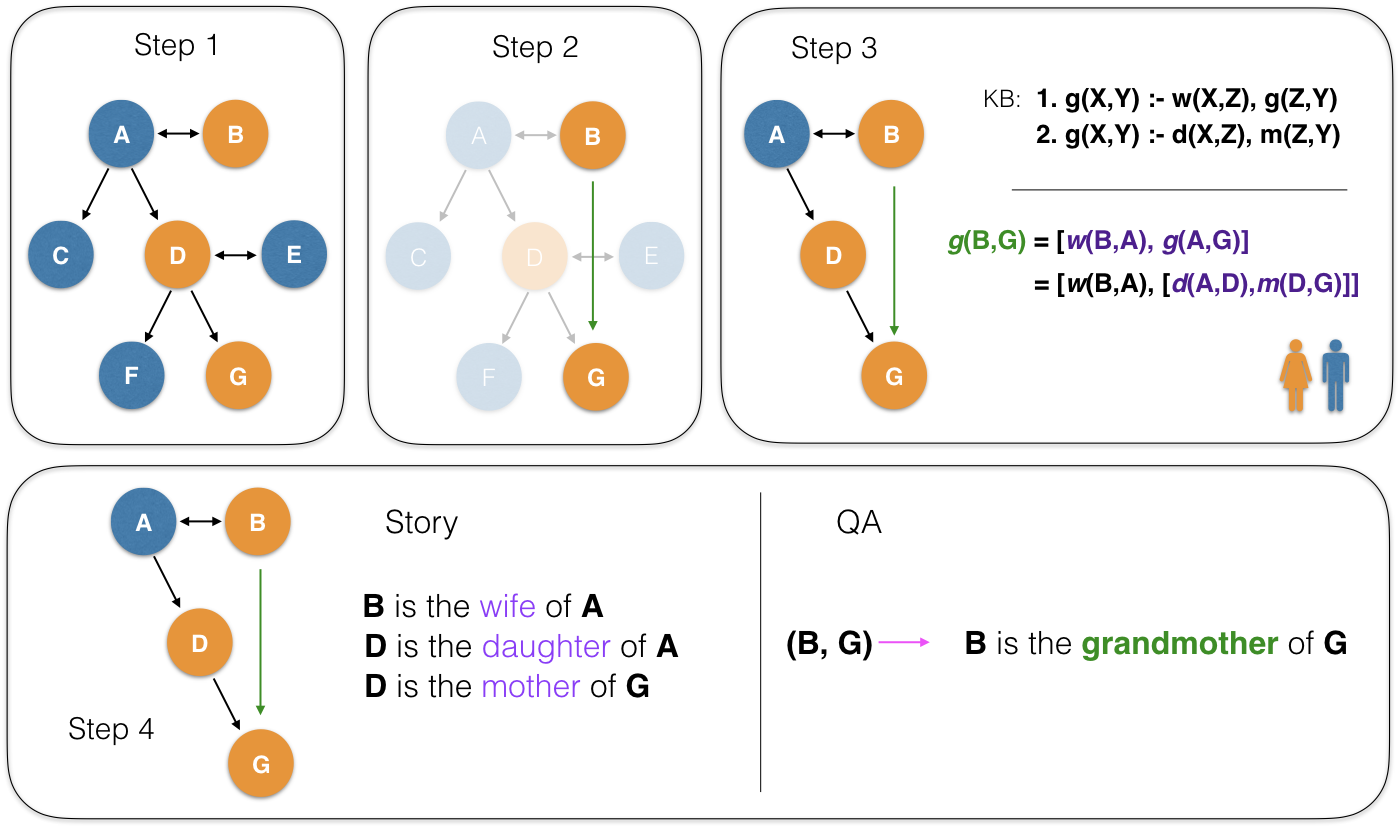
\includegraphics[]{figs/clutrr/dataset_const_new.png}}
\caption{Data generation pipeline. Step 1: generate a kinship graph. Step 2: sample a target fact. Step 3: Use backward chaining to sample a set of facts. Step 4: Convert sampled facts to a natural language story.}
\label{fig:clutrr:data}
\end{figure}


The core idea behind the CLUTRR benchmark suite is the following: Given a natural language story describing a set of kinship relations, the goal is to infer the relationship between two entities, whose relationship is {\em not} explicitly stated in the story.
To generate these stories, we first design a knowledge base (KB) with rules specifying how kinship relations resolve, and we use the following steps to create semi-synthetic stories based on this knowledge base:
\begin{enumerate}[topsep=3pt, parsep=6pt, leftmargin=40pt, itemsep=0pt, label={\bf Step \arabic*.}]
    \item \textbf{Generate} a random kinship graph that satisfies the rules in our KB.
    \item
        \textbf{Sample a target fact} (i.e., relation) to predict from the kinship graph.
    \item
        \textbf{Apply backward chaining} to sample a set of facts that can prove the target relation (and optionally sample a set of ``distracting'' or ``irrelevant'' noise facts).
    \item
        \textbf{Convert the sampled facts into a natural language story} through pre-specified text templates and crowd-sourced paraphrasing.
\end{enumerate}

Figure \ref{fig:clutrr:data} provides a high-level overview of this idea, and the following subsections describe the data generation process in detail, as well as the diagnostic flexibility afforded by CLUTRR.


% \subsection{Dataset construction}
% \label{sec:clutrr_data_const}

The short stories in CLUTRR are essentially narrativized renderings of a set of logical facts.
In the following sections, we describe how we sample the logical facts that make up a story by generating random kinship graphs and using backward chaining to produce logical reasoning chains.

% \subsection{Terminology and background}

\subsection{Graph generation}

%We restrict the set of rules in $R$ to consist of two atoms in the body (see the Appendix for the full set of rules).
% Using the logical rules in $R$ (see the Appendix for the full set of rules), we build a \textit{clause} which can be a conjunction of one or multiple rules.  %Further, we consider only binary predicates that make it easy to define a graph structure on the story.

To generate a kinship graph (say, $G$) underlying a particular story, we first sample a set of gendered\footnote{Kinship and gender roles are oversimplified in our data (compared to the real world) to maintain tractability.} entities and kinship relations using a stochastic generation process.
This generation process contains a number of tunable parameters---such as the maximum number of children at each node, the probability of an entity being married to another entity, etc.---and is designed to produce a valid, but possibly incomplete ``backbone graph''.
For instance, this backbone graph generation process will specify ``parent''/``child'' relations between entities but does not add ``grandparent'' relations.
After this initial generation process, we recursively apply the logical rules in $R$ to the backbone graph to produce a final graph $G$ that contains the full set of kinship relations between all the entities.
\footnote{In the context of our data generation process, we distinguish between the knowledge base, $R$, which contains a finite number of predicates and rules specifying how kinship relations in a family resolve, and a particular kinship graph $G$, which contains a grounded set of atoms specifying the particular kinship relations that underlie a single story.
In other words, $R$ contains the logical rules that govern all the generated stories in CLUTRR, while $G$ contains the grounded facts that underlie a specific story.}

In the CLUTRR Benchmark, the following kinship relations are used: \textit{son, father, husband, brother, grandson, grandfather, son-in-law, father-in-law, brother-in-law, uncle, nephew, daughter, mother, wife, sister, granddaughter, grandmother, daughter-in-law, mother-in-law, sister-in-law, aunt, niece}.

\footnotesize
\begin{align*}
\begin{split}
    [\texttt{grand}, X,Y] &\vdash [[\texttt{child}, X,Z],[\texttt{child}, Z,Y]], \\
    [\texttt{grand}, X,Y] &\vdash [[\texttt{SO}, X,Z],[\texttt{grand}, Z,Y]], \\
    [\texttt{grand}, X,Y] &\vdash [[\texttt{grand}, X,Z], [\texttt{sibling}, Z,Y]], \\
    [\texttt{inv-grand}, X,Y] &\vdash [[\texttt{inv-child}, X,Z], [\texttt{inv-child}, Z,Y]], \\
    [\texttt{inv-grand}, X,Y] &\vdash [[\texttt{sibling}, X,Z], [\texttt{inv-grand}, Z,Y]], \\
    [\texttt{child}, X,Y] &\vdash [[\texttt{child}, X,Z], [\texttt{sibling}, Z,Y]], \\
  [\texttt{child}, X,Y] &\vdash [[\texttt{SO}, X,Z], [\texttt{child}, Z,Y]], \\
  [\texttt{inv-child}, X,Y] &\vdash [[\texttt{sibling}, X,Z], [\texttt{inv-child}, Z,Y]], \\
    [\texttt{inv-child}, X,Y] &\vdash [[\texttt{child}, X,Z], [\texttt{inv-grand}, Z,Y]], \\
    [\texttt{sibling}, X,Y] &\vdash [[\texttt{child}, X,Z], [\texttt{inv-un}, Z,Y]], \\
    [\texttt{sibling}, X,Y] &\vdash [[\texttt{inv-child}, X,Z], [\texttt{child}, Z,Y]] \\
    [\texttt{sibling}, X,Y] &\vdash [[\texttt{sibling}, X,Z],[\texttt{sibling}, Z,Y]], \\
    [\texttt{in-law}, X,Y] &\vdash [[\texttt{child}, X,Z],[\texttt{SO}, Z,Y]], \\
    [\texttt{inv-in-law}, X,Y] &\vdash [[\texttt{SO}, X,Z],[\texttt{inv-child}, Z,Y]], \\
    [\texttt{un}, X,Y] &\vdash [[\texttt{sibling}, X,Z],[\texttt{child}, Z,Y]], \\
    [\texttt{inv-un}, X,Y] &\vdash [[\texttt{inv-child}, X,Z],[\texttt{sibling}, Z,Y]], \\
\end{split}
\end{align*}
\normalsize


We used a small, tractable, and logically sound KB of rules as mentioned above. We carefully select this set of deterministic rules to avoid ambiguity in the resolution. We use gender-neutral predicates and resolve the gender of the predicate in the head $\mathcal{H}$ of a clause $\mathcal{C}$ by deducing the gender of the second constant. We have two types of predicates, \textit{vertical} predicates (parent-child relations) and  \textit{horizontal} predicates (sibling or significant other). We denote all the vertical predicates by its \textit{child-to-parent} relation and append the prefix \texttt{inv-} to the predicates for the corresponding \textit{parent-to-child} relation. For example, \texttt{grandfatherOf} is denoted by the gender-neutral predicate $[\texttt{inv-grand},X,Y]$, where the gender is determined by the gender of $Y$.



\subsection{Backward chaining}
The resulting graph $G$ provides the \textit{background knowledge} for a specific story, as each edge in this graph can be treated as a grounded predicate (i.e., fact) between two entities.
From this graph $G$, we sample the facts that make up the story, as well as the target fact that we seek to predict:
First, we (uniformly) sample a target relation $\mathcal{H}_{\mathcal{C}}$, which is the fact that we want to predict from the story.
Then, from this target relation $\mathcal{H}_{\mathcal{C}}$,  we run a simple variation of the backward chaining \citep{gallaire1978logic} algorithm for $k$ iterations starting from $\mathcal{H}_{\mathcal{C}}$, where at each iteration we uniformly sample a subgoal to resolve and then uniformly sample a KB rule that resolves this subgoal.
Crucially, unlike traditional backward chaining, we do not stop the algorithm when a proof is obtained; instead, we run for a fixed number of iterations $k$ in order to sample a set of $k$ facts $\mathcal{B}_{\mathcal{C}}$ that imply the target relation $\mathcal{H}_{\mathcal{C}}$.

\subsection{Adding natural language}
\label{subsec:clutrr_nat_lang}

So far, we have described the process of generating a  conjunctive logical clause $\mathcal{C}=(\mathcal{H}_{\mathcal{C}} \vdash \mathcal{B}_{\mathcal{C}})$, where $\mathcal{H}_{\mathcal{C}}=[\alpha^*]$ is the target fact (i.e., relation) we seek to predict and $\mathcal{B}_{\mathcal{C}} = [\alpha_1, ..., \alpha_k]$ is the set of supporting facts that imply the target relation.
We now describe how we convert this logical representation to natural language through crowd-sourcing.

\subsubsection{Paraphrasing using Amazon Mechanical Turk}

We use Amazon Mechanical Turk (AMT), an online platform for collecting annotations from crowd-workers \footnote{\href{https://www.mturk.com/}{https://www.mturk.com/}}. The platform supports a mechanism to quickly annotate large amounts of data by paying anonymous workers for their effort. In our work, the crowd-workers are shown a set of facts $\mathcal{B}_{\mathcal{C}}$ corresponding to a story and then they are asked to paraphrase these facts into a narrative.
Since workers are given a set of facts $\mathcal{B}_{\mathcal{C}}$ to work from, they are able to combine and split multiple facts across separate sentences and construct diverse narratives (Figure \ref{fig:clutrr:lang_composition}).

We use ParlAI \citep{miller2017parlai} Mturk interface to collect paraphrases from the users. Specifically, given a set of facts, we ask the users to paraphrase the facts into a story. The users (\textit{turkers}) are free to construct any story they like as long as they mention all the entities and all the relations among them. We also provide the head $\mathcal{H}$ of the clause as an \textit{inferred} relation and specifically instruct the users to \textit{not} mention it in the paraphrased story. In order to evaluate the paraphrased stories, we ask the turkers to peer review a story paraphrased by a different turker. Since there are two tasks - paraphrasing a story and rating a story - we choose to pay 0.5\$ for each annotation. A sample task description in our MTurk interface is as follows:

\begin{quote}\small
    In this task, you will need to write a short, simple story based on a few facts. \textbf{It is crucial that the story mentions each of the given facts at least once.} The story does not need to be complicated! It just needs to be grammatical and mention the required facts.

    After writing the story, you will be asked to evaluate the quality of a generated story (based on a different set of facts). \textbf{It is crucial that you check whether the generated story mentions each of the required facts.}

    \textit{Example of good and bad stories: Good Example}

    \textbf{Facts to Mention}
    \begin{itemize}
        \item John is the father of Sylvia.
        \item Sylvia has a brother Patrick.
    \end{itemize}

    \textbf{Implied Fact}: John is the father of Patrick.

    \textbf{Written story}

    John is the proud father of the lovely Sylvia. Sylvia has a love-hate relationship with her brother Patrick.

    \textit{Bad Example}

    \textbf{Facts to Mention}

    \begin{itemize}
        \item Vincent is the son of Tim.
        \item Martha is the wife of Tim.
    \end{itemize}

    \textbf{Implied Fact} : Martha is Vincent's mother.

    \textbf{Written story}

    Vincent is married at Tim and his mother is Martha.

    \textit{The reason the above story is bad}:

    \begin{itemize}
        \item This story is bad because it is nonsense / ungrammatical.
        \item This story is bad because it does not mention the proper facts.
        \item This story is bad because it reveals the implied fact.
    \end{itemize}
\end{quote}

A sample of the AMT interface is shown in \autoref{fig:clutrr:mturk}.
To ensure that the turkers are providing high-quality annotations without revealing the inferred fact, we also launch another task to ask the turkers to rate three annotations to be either good or bad which are provided by a set of \textit{different} turkers. We pay 0.2\$ for each HIT consisting of three reviews. This helped to remove logical and grammatical inconsistencies to a large extent. Based on the reviews, 79\% of the collected paraphrases passed the peer-review sanity check where all the reviewers agree on the quality. This subset of the placeholders is used in the benchmark. A sample of programmatically generated dataset for clause length of $k=2$ to $k=6$ is provided in the tables \ref{tab:puzzle_data_1} to \ref{tab:puzzle_data_5}.

\begin{figure*}[h]
  \centering
  \resizebox{0.8\textwidth}{!}{
    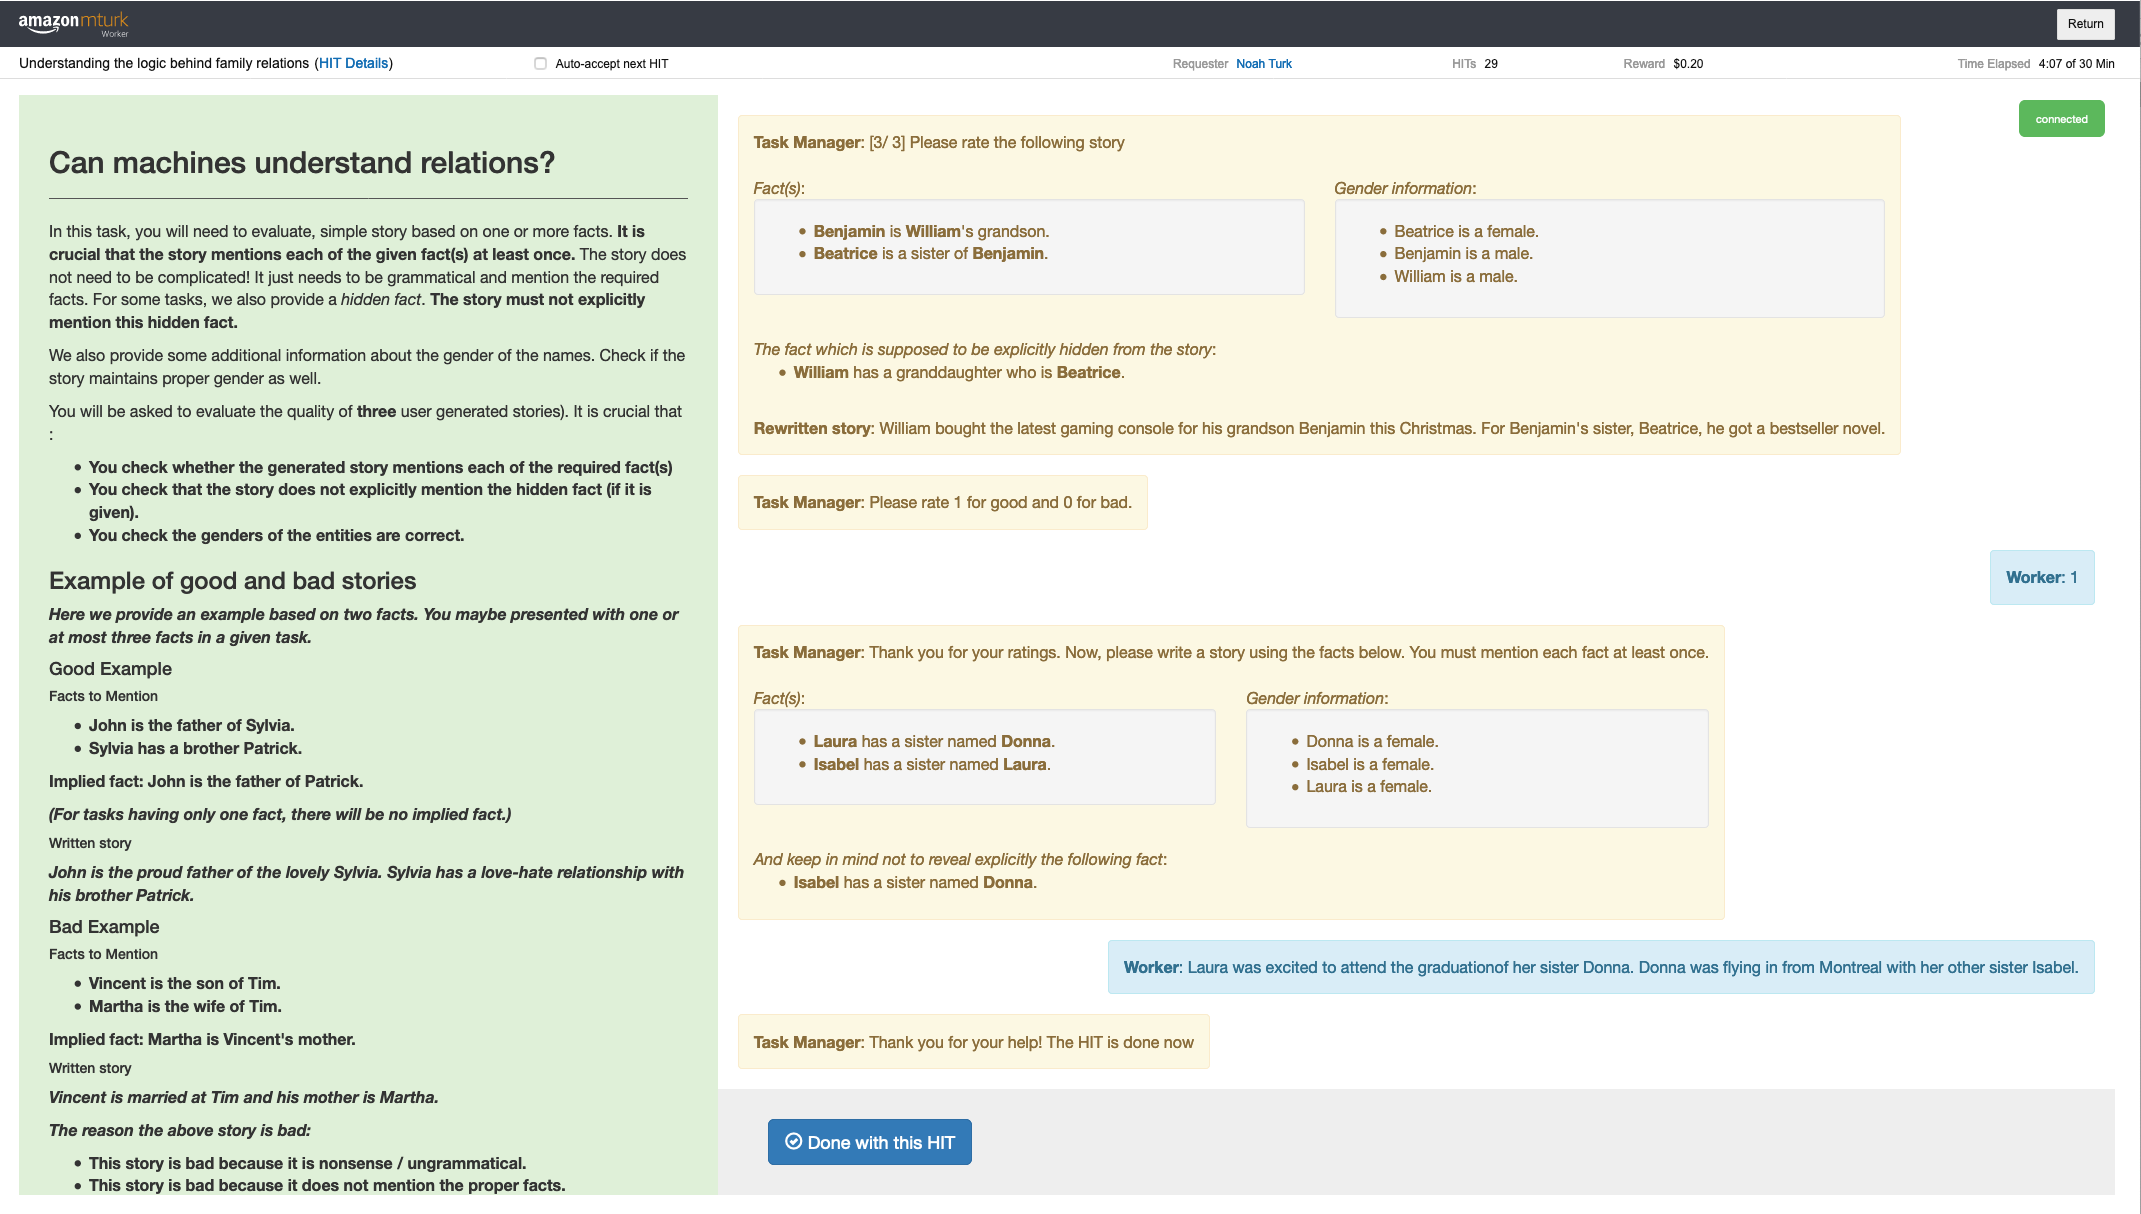
\includegraphics[width=\textwidth]{figs/clutrr/mturk_interface.png}}
    \caption{Amazon Mechanical Turker Interface built using ParlAI which was used to collect data as well as peer reviews.}%
    \label{fig:clutrr:mturk}
\end{figure*}



\subsubsection{Reusability and composition}
One challenge for data collection via AMT is that the number of possible stories generated by CLUTRR grows combinatorially as the number of supporting facts increases, i.e., as  $k=|\mathcal{B}_{\mathcal{C}}|$ grows.
This combinatorial explosion for large $k$---combined with the difficulty of maintaining the quality of the crowd-sourced paraphrasing for long stories---makes it infeasible to obtain a large number of paraphrased examples for $k>3$.
To circumvent this issue and increase the flexibility of our benchmark, we reuse and compose AMT paraphrases to generate longer stories.
In particular, we collected paraphrases for stories containing $k=1,2,3$ supporting facts and then replaced the entities from these collected stories with placeholders in order to re-use them to generate longer semi-synthetic stories.
An example of a story generated by stitching together two shorter paraphrases is provided below:
\vspace{-5pt}
\begin{quote}{\small
    [Frank] went to the park with his father, [Brett]. [Frank] called his brother [Boyd] on the phone. He wanted to go out for some beers.
    [Boyd] went to the baseball game with his son [Jim].\\
    Q: What is [Brett] and [Jim]'s relationship?}
\end{quote}
\vspace{-5pt}
Thus, instead of simply collecting paraphrases for a fixed number of stories, we instead obtain a diverse collection of natural language templates that can be programmatically recombined to generate stories with various properties.

\subsection{AMT Template statistics}


\begin{table}[]
\centering
\resizebox{0.48\textwidth}{!}{%
\begin{tabular}{@{}rrll@{}}
\toprule
\multicolumn{1}{l}{Number of Paraphrases} & \multicolumn{1}{l}{} &  & \# clauses \\ \midrule
\multicolumn{1}{r|}{} & $k$ = 1 & 1,868 & \multicolumn{1}{c}{20} \\
\multicolumn{1}{r|}{} & $k$ = 2 & 1,890 & \multicolumn{1}{c}{58} \\
\multicolumn{1}{r|}{} & $k$ = 3 & 2,258 & \multicolumn{1}{c}{236} \\ \cmidrule(l){2-4} 
\multicolumn{1}{r|}{} & Total & 6,016 &  \\ \midrule
\multicolumn{1}{l}{Unique Word Count} &  & 3,797 &  \\ \midrule
\multicolumn{1}{r|}{Jaccard Word Overlap} & Unigrams & 0.201 &  \\
\multicolumn{1}{r|}{} & Bigrams & 0.0385 &  \\ \bottomrule
\end{tabular}%
}
\caption{Statistics of the AMT paraphrases. Jaccard word overlap is calculated within the templates of each individual clause of length $k$.}
\label{tab:placeholder}
\end{table}


At the time of submission, we have collected 6,016 unique paraphrases with an average of 19 paraphrases for every possible logical clause of length $k=1,2,3$. Table \ref{tab:placeholder} contains summary statistics of the collected paraphrases.
Overall, we found high linguistic diversity in the collected paraphrases.
For instance, the average Jaccard overlap in unigrams between pairs paraphrases corresponding to the same logical clause was only 0.201 and only 0.0385 for bigrams.

\subsection{Human performance}

% Please add the following required packages to your document preamble:
% \usepackage{booktabs}
% \usepackage{multirow}
% \usepackage{graphicx}
\begin{table}[]
\centering
\resizebox{0.7\textwidth}{!}{%
\begin{tabular}{@{}llll@{}}
\toprule
\multirow{2}{*}{Relation Length} & \multicolumn{2}{l}{Human Performance} & \multirow{2}{*}{Reported Difficulty} \\
 & Time Limited & Unlimited Time &  \\ \midrule
2 & 0.848 & 1 & 1.488 +- 1.25 \\
3 & 0.773 & 1 & 2.41 +- 1.33 \\
4 & 0.477 & 1 & 3.81 +- 1.46 \\
5 & 0.424 & 1 & 3.78 +- 0.96 \\
6 & 0.406 & 1 & 4.46 +- 0.87 \\ \bottomrule
\end{tabular}%
}
\caption{Human performance accuracies on CLUTRR dataset. Humans are provided the Clean-Generalization version of the dataset, and we test on two scenarios: when a human is given limited time to solve the task, and when a human is given unlimited time to solve the task. Regardless of time, our evaluators provide a score of difficulty of individual puzzles.}
\label{tab:clutrr:human_perf}
\end{table}


To get a sense of the data quality and difficulty involved in CLUTRR, we asked human annotators to solve the task for random examples of length $k=2,3,...,6$. (\autoref{tab:clutrr:human_perf})
We perform the evaluation in two scenarios: first a time-limited scenario where we ask AMT Turkers to solve the puzzle in a fixed time. Turkers were provided a maximum time of 30 mins, but they solved the puzzles in an average of 1 minute 23 seconds. Secondly, we use another set of expert evaluators who are given ample time to solve the tasks. Not surprisingly, if a human being is given ample time (experts took an average of 6 minutes per puzzle) and a pen and a paper to aid in the reasoning, they get all the relations correct. However, if an evaluator is short of time, they might miss important details on the relations and perform poorly. Thus, our tasks require \textit{active attention}.

We found that time-constrained AMT annotators performed well (i.e., ${>70\%}$) accuracy for ${k\leq 3}$ but struggled with examples involving longer stories, achieving 40-50\% accuracy for ${k > 3}$. However, trained annotators with unlimited time were able to solve 100\% of the examples, highlighting the fact that this task requires attention and involved reasoning, even for humans.

\subsection{Representing the question and entities}

The AMT paraphrasing approach described above allows us to convert the set of supporting facts $\mathcal{B}_{\mathcal{C}}$ to a natural language story, which can be used to predict the target relation/query $\mathcal{H}_{\mathcal{C}}$.
However, instead of converting the target query, $\mathcal{H}_{\mathcal{C}} = [\alpha^*]$, to a natural language question, we instead opt to represent the target query as a $K$-way classification task, where the two entities in the target relation are provided as input and the goal is to classify the relation that holds between these two entities.
This representation avoids the pitfall of revealing information about the answer in the question \citep{kaushik2018much}.

When generating stories, entity names are randomly drawn from a set of 300 common gendered English names.
Thus, depending on each run, the entities are never the same.
This ensures that the entity names are simply placeholders and uncorrelated from the task.



\begin{figure}[t]
\centering
\resizebox{0.45\textwidth}{!}{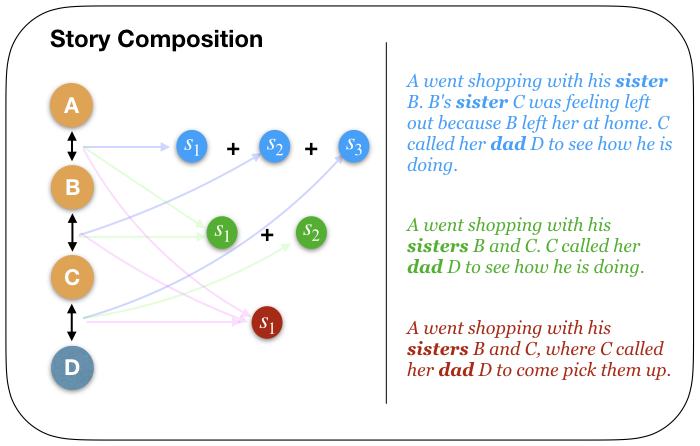
\includegraphics[]{figs/clutrr/composition.png}}
\caption{Illustration of how a set of facts can split and combined in various ways across sentences.}
\label{fig:clutrr:lang_composition}
\end{figure}


\begin{figure}[t]
\centering
\resizebox{0.38\textwidth}{!}{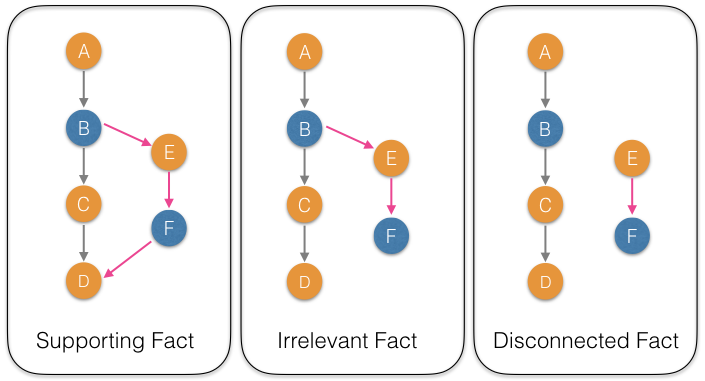
\includegraphics[]{figs/clutrr/clutrr_noise.png}}
\caption{Noise generation procedures of CLUTRR.}
\label{fig:clutrr:data_noise}
\end{figure}



\section{Experimental Setups}
\label{sec:clutrr_setups}

The modular nature of CLUTRR provides rich diagnostic capabilities for evaluating the robustness and generalization abilities of neural language understanding systems.
We highlight some key diagnostic capabilities available via different variations of CLUTRR below.
These diagnostic variations correspond to the concrete datasets that we generated in this work, and we describe the results on these datasets in \autoref{sec:clutrr_results}.

\subsection{Systematic generalization}

Most prominently, CLUTRR allows us to explicitly evaluate a model's ability for generalizing with the property of systematicity.
In particular, we rely on the following hold-out procedures to test systematic generalization:
\begin{itemize}[leftmargin=*, topsep=2pt, itemsep=2pt, parsep=2pt]
    \item During training, we hold out a subset of the collected paraphrases, and we only use this held-out subset of paraphrases when generating the test set.
    Thus, to succeed on CLUTRR, an \acrshort{nlu} system must exhibit {\em linguistic generalization} and be robust to linguistic variation at test time.
    \item We also hold out a subset of the logical clauses during training (for clauses of length $k > 2$).\footnote{One should not holdout clauses from length $k=2$ in order to allow models to learn the compositionality of all possible binary predicates.}
    In other words, during training, the model sees all logical rules but does not see all {\em combinations} of these logical rules.
    Thus, in addition to linguistic generalization, success on this task also requires {\em logical generalization}.
    \item
    Lastly, as a more extreme form of both logical and linguistic generalization, we consider the setting where the models are trained on stories generated from clauses of length ${\leq k}$ and evaluated on stories generated from larger clauses of length ${>k}$. Thus, we explicitly test the ability for models to generalize on examples that require more steps of reasoning that any example they encountered during training.
\end{itemize}

\subsection{Robust Reasoning}
\label{sec:clutrr_robust_data}

In addition to evaluating systematic generalization, the modular setup of CLUTRR also allows us to diagnose model robustness by adding \textit{noise facts} to the generated narratives.
Due to the controlled semi-synthetic nature of CLUTRR, we are able to provide a precise taxonomy of the kinds of noise facts that can be added (Figure \ref{fig:clutrr:data_noise}).
In order to structure this taxonomy, it is important to recall that any set of supporting facts $\mathcal{B}_{\mathcal{C}}$ generated by CLUTRR can be interpreted as a path, $p_{\mathcal{C}}$, in the corresponding kinship graph $G$ (Figure \ref{fig:clutrr:data}).
Based on this interpretation, we view adding noise facts from the perspective of sampling three different types of noise paths, $p_n$, from the kinship graph $G$:
\begin{itemize}[  leftmargin=10pt, topsep=0pt, itemsep=0pt, parsep=0pt]
    \item \textit{Irrelevant facts}: We add a path $p_n$, which has exactly one shared end-point with $p_c$. In this way, this is a \textit{distractor} path,
    which contains facts that are connected to one of the entities in the target relation, $\mathcal{H}_{\mathcal{C}}$, but do not provide any information that could be used to help answer the query. %We name this task \texttt{CLUTRR-Irrelevant}
     \item \textit{Supporting facts}:
    We add a path $p_n$, whose two end-points are on the path $p_{\mathcal{C}}$.
    The facts on this path $p_n$ are noise because they are not needed to answer the query, but they are supporting facts because they can, in principle, be used to construct alternative (longer) reasoning paths that connect the two target entities.
    %We denote this setup as \texttt{CLUTRR-Supporting}
    \item \textit{Disconnected facts}: We add paths which neither originate nor end in any entity on $p_c$. These disconnected facts involve entities and relations that are completely unrelated to the target query.
    %We call this variant \texttt{CLUTRR-Disconnected}.
\end{itemize}

\subsection{Generated Datasets}

For all experiments, we generated datasets with 10-15k training examples.
In many experiments, we report training and testing results on stories with different clause lengths $k$.
(For brevity, we use the phrase ``clause length'' throughout this section to refer to the value $k=|\mathcal{B}_{\mathcal{C}}|$, i.e., the number of steps of reasoning that are required to predict the target query.)
In all cases, the training set contains 5000 train stories per $k$ value, and, during testing, all experiments use 100 test stories per $k$ value.
All experiments were run 10 times with different randomly generated stories, and means and standard errors over these 10 runs are reported.
As discussed above, during training we holdout 20\% of the paraphrases, as well as 10\% of the possible logical clauses.


% Please add the following required packages to your document preamble:
% \usepackage{booktabs}
% \usepackage{graphicx}
\begin{table*}[]
\centering
\caption{Snapshot of puzzles in the dataset for k=2}
\label{tab:puzzle_data_1}
\resizebox{0.7\textwidth}{!}{%
\begin{tabular}{@{}p{7cm}lll@{}}
\toprule
\textbf{Puzzle} & \textbf{Question} & \textbf{Gender} & \textbf{Answer} \\ \midrule
\addlinespace[0.5em]
\noindent\parbox[c]{\hsize}{\textit{Charles}'s son \textit{Christopher} entered rehab for the ninth time at the age of thirty. \textit{Randolph} had a nephew called \textit{Christopher} who had n't seen for a number of years.} & Randolph is the \_\_\_\_\_ of Charles & \begin{tabular}[c]{@{}l@{}}Charles:male,\\ Christopher:male,\\ Randolph:male\end{tabular} & brother \\
\addlinespace[0.5em]
\noindent\parbox[c]{\hsize}{\textit{Randolph} and his sister \textit{Sharon} went to the park. \textit{Arthur} went to the baseball game with his son \textit{Randolph}}. & Sharon is the \_\_\_\_\_ of Arthur & \begin{tabular}[c]{@{}l@{}}Arthur:male,\\ Randolph:male,\\ Sharon:female\end{tabular} & daughter \\
\addlinespace[0.5em]
\noindent\parbox[c]{\hsize}{\textit{Frank} went to the park with his father, \textit{Brett}. \textit{Frank} called his brother \textit{Boyd} on the phone. He wanted to go out for some beers.} & Brett is the \_\_\_\_\_ of Boyd & \begin{tabular}[c]{@{}l@{}}Boyd:male,\\ Frank:male,\\ Brett:male\end{tabular} & father \\ \bottomrule
\end{tabular}%
}
\end{table*}

% Please add the following required packages to your document preamble:
% \usepackage{booktabs}
% \usepackage{graphicx}
\begin{table*}[]
\centering
\caption{Snapshot of puzzles in the dataset for k=3}
\label{tab:puzzle_data_2}
\resizebox{0.7\textwidth}{!}{%
\begin{tabular}{@{}p{7cm}lll@{}}
\toprule
\textbf{Puzzle} & \textbf{Question} & \textbf{Gender} & \textbf{Answer} \\ \midrule
\textit{Roger} was playing baseball with his sons \textit{Sam} and \textit{Leon}. \textit{Sam} had to take a break though because he needed to call his sister \textit{Robin}. & Leon is the \_\_\_\_\_ of Robin & \begin{tabular}[c]{@{}l@{}}Robin:female,\\ Sam:male,\\ Roger:male,\\ Leon:male\end{tabular} & brother \\
\textit{Elvira} and her daughter \textit{Nancy} went shopping together last Monday and they bought new shoes for \textit{Elvira}'s kids. \textit{Pedro} and his sister \textit{Allison} went to the fair. \textit{Pedro}'s mother, \textit{Nancy}, was out with friends for the day. & Elvira is the \_\_\_\_\_ of Allison & \begin{tabular}[c]{@{}l@{}}Allison:female,\\ Pedro:male,\\ Nancy:female,\\ Elvira:female\end{tabular} & grandmother \\
\textit{Roger} met up with his sister \textit{Nancy} and her daughter \textit{Cynthia} at the mall to go shopping together. \textit{Cynthia}'s brother \textit{Pedro} was going to be the star in the new show. & Pedro is the \_\_\_\_\_ of Roger & \begin{tabular}[c]{@{}l@{}}Roger:male,\\ Nancy:female,\\ Cynthia:female,\\ Pedro:male\end{tabular} & nephew \\ \bottomrule
\end{tabular}%
}
\end{table*}

% Please add the following required packages to your document preamble:
% \usepackage{booktabs}
% \usepackage{graphicx}
\begin{table*}[]
\centering
\caption{Snapshot of puzzles in the dataset for k=4}
\label{tab:puzzle_data_3}
\resizebox{0.7\textwidth}{!}{%
\begin{tabular}{@{}p{7cm}lll@{}}
\toprule
\textbf{Puzzle} & \textbf{Question} & \textbf{Gender} & \textbf{Answer} \\ \midrule
\textit{Celina} has been visiting her sister, \textit{Fran} all week. \textit{Fran} is also the daughter of \textit{Bethany}. \textit{Ronald} loves visiting his aunt \textit{Bethany} over the weekends. \textit{Samuel}'s son \textit{Ronald} entered rehab for the ninth time at the age of thirty. & Celina is the \_\_\_\_\_ of Samuel & \begin{tabular}[c]{@{}l@{}}Samuel:male,\\ Ronald:male,\\ Bethany:female,\\ Fran:female,\\ Celina:female\end{tabular} & niece \\
\textit{Celina} adores her daughter \textit{Bethany}. \textit{Bethany} loves her very much, too. \textit{Jackie} called her mother \textit{Bethany} to let her know she will be back home soon. \textit{Thomas} was helping his daughter \textit{Fran} with her homework at home. Afterwards, \textit{Fran} and her sister \textit{Jackie} played Xbox together. & Celina is the \_\_\_\_\_ of Thomas & \begin{tabular}[c]{@{}l@{}}Thomas:male,\\ Fran:female,\\ Jackie:female,\\ Bethany:female,\\ Celina:female\end{tabular} & daughter \\
\textit{Raquel} is \textit{Samuel} 'daughter and they go shopping at least twice a week together. \textit{Kenneth} and her mom, \textit{Theresa}, had a big fight. \textit{Theresa}'s son, \textit{Ronald}, refused to get involved. \textit{Ronald} was having an argument with her sister, \textit{Raquel}. & Samuel is the \_\_\_\_\_ of Kenneth & \begin{tabular}[c]{@{}l@{}}Kenneth:male,\\ Theresa:female,\\ Ronald:male,\\ Raquel:female,\\ Samuel:male\end{tabular} & father \\ \bottomrule
\end{tabular}%
}
\end{table*}

% Please add the following required packages to your document preamble:
% \usepackage{booktabs}
% \usepackage{graphicx}
\begin{table*}[]
\centering
\caption{Snapshot of puzzles in the dataset for k=5}
\label{tab:puzzle_data_4}
\resizebox{0.7\textwidth}{!}{%
\begin{tabular}{@{}p{7cm}lll@{}}
\toprule
\textbf{Puzzle} & \textbf{Question} & \textbf{Gender} & \textbf{Answer} \\ \midrule
\textit{Steven}'s son is \textit{Bradford}. \textit{Bradford} and his father always go fishing together on Sundays and have a great time together. \textit{Diane} is taking her brother \textit{Brad} out for a late dinner. \textit{Kristin}, \textit{Brad}'s mother, is home with a cold. \textit{Diane}'s father \textit{Elmer}, and his brother \textit{Steven}, all got into the rental car to start the long cross-country roadtrip they had been planning. & Bradford is the \_\_\_\_\_ of Kristin & \begin{tabular}[c]{@{}l@{}}Kristin:female,\\ Brad:male,\\ Diane:female,\\ Elmer:male,\\ Steven:male,\\ Bradford:male\end{tabular} & nephew \\
\textit{Elmer} went on a roadtrip with his youngest child, \textit{Brad}. \textit{Lena} and her sister \textit{Diane} are going to a restaurant for lunch. \textit{Lena}'s brother \textit{Brad} is going to meet them there with his father \textit{Elmer} \textit{Brad} ca n't stand his unfriendly aunt \textit{Lizzie}. & Lizzie is the \_\_\_\_\_ of Diane & \begin{tabular}[c]{@{}l@{}}Diane:female,\\ Lena:female,\\ Brad:male,\\ Elmer:male,\\ Lizzie:female\end{tabular} & aunt \\
\textit{Ira} took his niece \textit{April} fishing Saturday. They caught a couple small fish. \textit{Ronald} was enjoying spending time with his parents, \textit{Damion} and \textit{Claudine}. \textit{Damion}'s other son, \textit{Dennis}, wanted to come visit too. \textit{Dennis} often goes out for lunch with his sister, \textit{April}. & Ira is the \_\_\_\_\_ of Claudine & \begin{tabular}[c]{@{}l@{}}Claudine:female,\\ Ronald:male,\\ Damion:male,\\ Dennis:male,\\ April:female,\\ Ira:male\end{tabular} & brother \\ \bottomrule
\end{tabular}%
}
\end{table*}

% Please add the following required packages to your document preamble:
% \usepackage{booktabs}
% \usepackage{graphicx}
\begin{table*}[]
\centering
\caption{Snapshot of puzzles in the dataset for k=6}
\label{tab:puzzle_data_5}
\resizebox{0.7\textwidth}{!}{%
\begin{tabular}{@{}p{7cm}lll@{}}
\toprule
\textbf{Puzzle} & \textbf{Question} & \textbf{Gender} & \textbf{Answer} \\ \midrule
\textit{Mario} wanted to get a good gift for his sister, \textit{Marianne}. \textit{Jean} and her sister \textit{Darlene} were going to a party held by \textit{Jean}'s mom, \textit{Marianne}. \textit{Darlene} invited her brother \textit{Roy} to come, too, but he was too busy. \textit{Teri} and her father, \textit{Mario}, had an argument over the weekend. However, they made up by Monday. \textit{Agnes} wants to make a special meal for her daughter \textit{Teri}'s birthday. & Roy is the \_\_\_\_\_ of Agnes & \begin{tabular}[c]{@{}l@{}}Agnes:female,\\ Teri:female,\\ Mario:male,\\ Marianne:female,\\ Jean:female,\\ Darlene:female,\\ Roy:male\end{tabular} & nephew \\
\textit{Robert}'s aunt, \textit{Marianne}, asked \textit{Robert} to mow the lawn for her. \textit{Robert} said he could n't because he had a bad back. \textit{William}'s parents, \textit{Brian} and \textit{Marianne}, threw him a surprise party for his birthday. \textit{Brian}'s daughter \textit{Jean} made a mental note to be out of town for her birthday! \textit{Agnes}'s biggest accomplishment is raising her son \textit{Robert}. \textit{Jean} is looking for a good gift for her sister \textit{Darlene}. & Darlene is the \_\_\_\_\_ of Agnes & \begin{tabular}[c]{@{}l@{}}Agnes:female,\\ Robert:male,\\ Marianne:female,\\ William:male,\\ Brian:male,\\ Jean:female,\\ Darlene:female\end{tabular} & niece \\
\textit{Sharon} and her brother \textit{Mario} went shopping. \textit{Teri}, \textit{Mario}'s daughter, came too. \textit{Agnes}, \textit{Annie}'s mother, is unhappy with \textit{Robert}. She feels her son is cruel to \textit{Annie}'s sister \textit{Teri}, and she wants \textit{Robert} to be nicer. \textit{Robert}'s sister, \textit{Nicole}, participated in the dance contest. & Nicole is the \_\_\_\_\_ of Sharon & \begin{tabular}[c]{@{}l@{}}Sharon:female,\\ Mario:male,\\ Teri:female,\\ Annie:female,\\ Agnes:female,\\ Robert:male,\\ Nicole:female\end{tabular} & niece \\ \bottomrule
\end{tabular}%
}
\end{table*}



\section{Evaluated Models}
\label{sec:clutrr_models}

Our primary baselines are neural language understanding models that take unstructured text as input.
We consider bidirectional LSTMs \citep{hochreiter1997long, cho2014learning} (with and without attention), as well as models that aim to incorporate inductive biases towards relational reasoning: Relation Networks (RN) \citep{santoro2017simple}, Relational Recurrent Networks (RMC) \citep{santoro2018relational} and Compositional Memory Attention Network (MAC) \citep{hudson2018compositional}. We also use the large pre-trained language model, BERT \citep{devlin-etal-2019-bert}, as well as a modified version of BERT having a trainable LSTM encoder on top of the pretrained BERT embeddings.
All of these models (except BERT) were re-implemented in PyTorch 1.0 \citep{paszke2017automatic} and adapted to work with the CLUTRR benchmark.

Since the underlying relations in the stories generated by CLUTRR inherently form a graph, we also experiment with a Graph Attention Network (GAT) \citep{Velickovic2017-mh}.
%Specifically, we consider }, as a representative model from the field of graph representation learning \cite{2017arXiv170905584H}.
Rather than taking the textual stories as input, the GAT baseline receives a structured graph representation of the facts that underlie the story.
%The motivation behind the inclusion of the GAT baseline is to evaluate the difficulty of the inductive reasoning task without the challenge of interpreting the natural language.
%these two classes of models is to present the two extremes in current relational reasoning space : unstructured models which has to construct a latent graph, compared with structured model having the perfect graph as input.
%Future explorations can target the space between these models where an information retrieval (IR) model \citep{schoenmackers2010learning} can be used to extract the underlying graph from text and fed into a reasoning model.


\xhdr{Entity and query representations}
We use the various baseline models to encode the natural language story (or graph) into a fixed-dimensional embedding.
With the exception of the BERT models, we do not use pre-trained word embeddings and learn the word embeddings from scratch using end-to-end backpropagation.
An important note, however, is that we perform Cloze-style anonymization \citep{hermann2015teaching} of the entities (i.e., names) in the stories, where each entity name is replaced by a \textit{@entity-k} placeholder, which is randomly sampled from a small, fixed pool of placeholder tokens. The embeddings for these placeholders are randomly initialized and fixed during training.

To make a prediction about a target query given a story, we concatenate the embedding of the story (generated by the baseline model) with the embeddings of the two target entities and we feed this concatenated embedding to a 2-layer feed-forward neural network with a softmax prediction layer.

\subsection{Hyperparameters}

For all models, the common hyperparameters used are: Embedding dimension: 100 (except BERT based models), Optimizer: Adam, Learning rate: 0.001, Number of epochs: 100, Number of runs: 10. Specific model-based hyperparameters are given as follows:

\begin{itemize}
    \item \textbf{Bidirectional LSTM} \citep{hochreiter1997long, cho2014learning}: LSTM hidden dimension: 100, \# layers: 2, Classifier MLP hidden dimension: 200
    \item \textbf{Relation Networks} \citep{santoro2017simple}: $f_{{\theta}_1}$ : 256, $f_{{\theta}_2}$: 64, $g_{\theta}$ : 64
    \item \textbf{Compositional Memory Attention Network (MAC)} \citep{hudson2018compositional}: \# Iterations: 6, \texttt{shareQuestion}: True, Dropout - Memory, Read and Write: 0.2
    \item \textbf{Relational Recurrent Networks} \citep{santoro2018relational}: Memory slots: 2, Head size: 192, Number of heads: 4, Number of blocks : 1, forget bias : 1, input bias: 0, gate style: unit, key size: 64, \# Attention layers: 3, Dropout: 0
    \item \textbf{BERT} \citep{devlin-etal-2019-bert}: Layers : 12, Fixed pretrained embeddings from \\ \texttt{bert-base-uncased} using Pytorch HuggingFace BERT repository \footnote{\href{https://github.com/huggingface/pytorch-pretrained-BERT}{https://github.com/huggingface/pytorch-pretrained-BERT}}, Word dimension: 768, appended with a two-layer MLP for final prediction.
    \item \textbf{BERT-LSTM}: Same parameters as above, with a two-layer unidirectional LSTM encoder on top of BERT word embeddings.
    \item \textbf{GAT} \citep{Velickovic2017-mh}: Node dimension: 100, Message dimension: 100, Edge dimension: 20, number of rounds: 3
\end{itemize}



\section{Results}
\label{sec:clutrr_results}

We evaluate several \acrshort{nlu} systems on the proposed CLUTRR benchmark to surface the relative strengths and shortcomings of these models in the context of inductive reasoning and combinatorial generalization.\footnote{Code to reproduce all the results in this section are available at  \href{https://github.com/facebookresearch/clutrr/}{https://github.com/facebookresearch/clutrr/}.} We aim to answer the following key questions:
\begin{enumerate}[label=({\bf Q\arabic*}), leftmargin=28pt, topsep=0pt, itemsep=0pt, parsep=0pt]
\item How do state-of-the-art \acrshort{nlu} models compare in terms of systematic generalization? Can these models generalize to stories with unseen combinations of logical rules?
 \item How does the performance of neural language understanding models compare to a graph neural network that has full access to graph structure underlying the stories?
    \item How robust are these models to the addition of noise facts to a given story?
\end{enumerate}

\subsection{Systematic Generalization}
\label{sec:clutrr_sys_gen}

We begin by using CLUTRR to evaluate the ability of the baseline models to perform systematic generalization (\textbf{Q1}).
In this setting, we consider two training regimes: in the first regime, we train all models with clauses of length $k=2,3$, and in the second regime, we train with clauses of length $k=2,3,4$.
We then test the generalization of these models on test clauses of length $k=2,...,10$.

Figure \ref{fig:gen_1} illustrates the performance of different models on this generalization task.
We observe that the GAT model is able to perform near-perfectly on the held-out logical clauses of length $k=3$, with the BERT-LSTM being the top-performer among the text-based models but still significantly below the GAT.
Not surprisingly, the performance of all models degrades monotonically as we increase the length of the test clauses, which highlights the challenge of ``zero-shot'' systematic generalization \cite{Lake2018:SCAN, 2018arXiv181107017S}.
However, as expected, all models improve on their generalization performance when trained on $k=2,3,4$ rather than just $k=2,3$ (Figure \ref{fig:gen_1}, right). The GAT, in particular, achieves the biggest gain by this expanded training.

\begin{figure*}[!htb]
     \centering
    \subfloat{{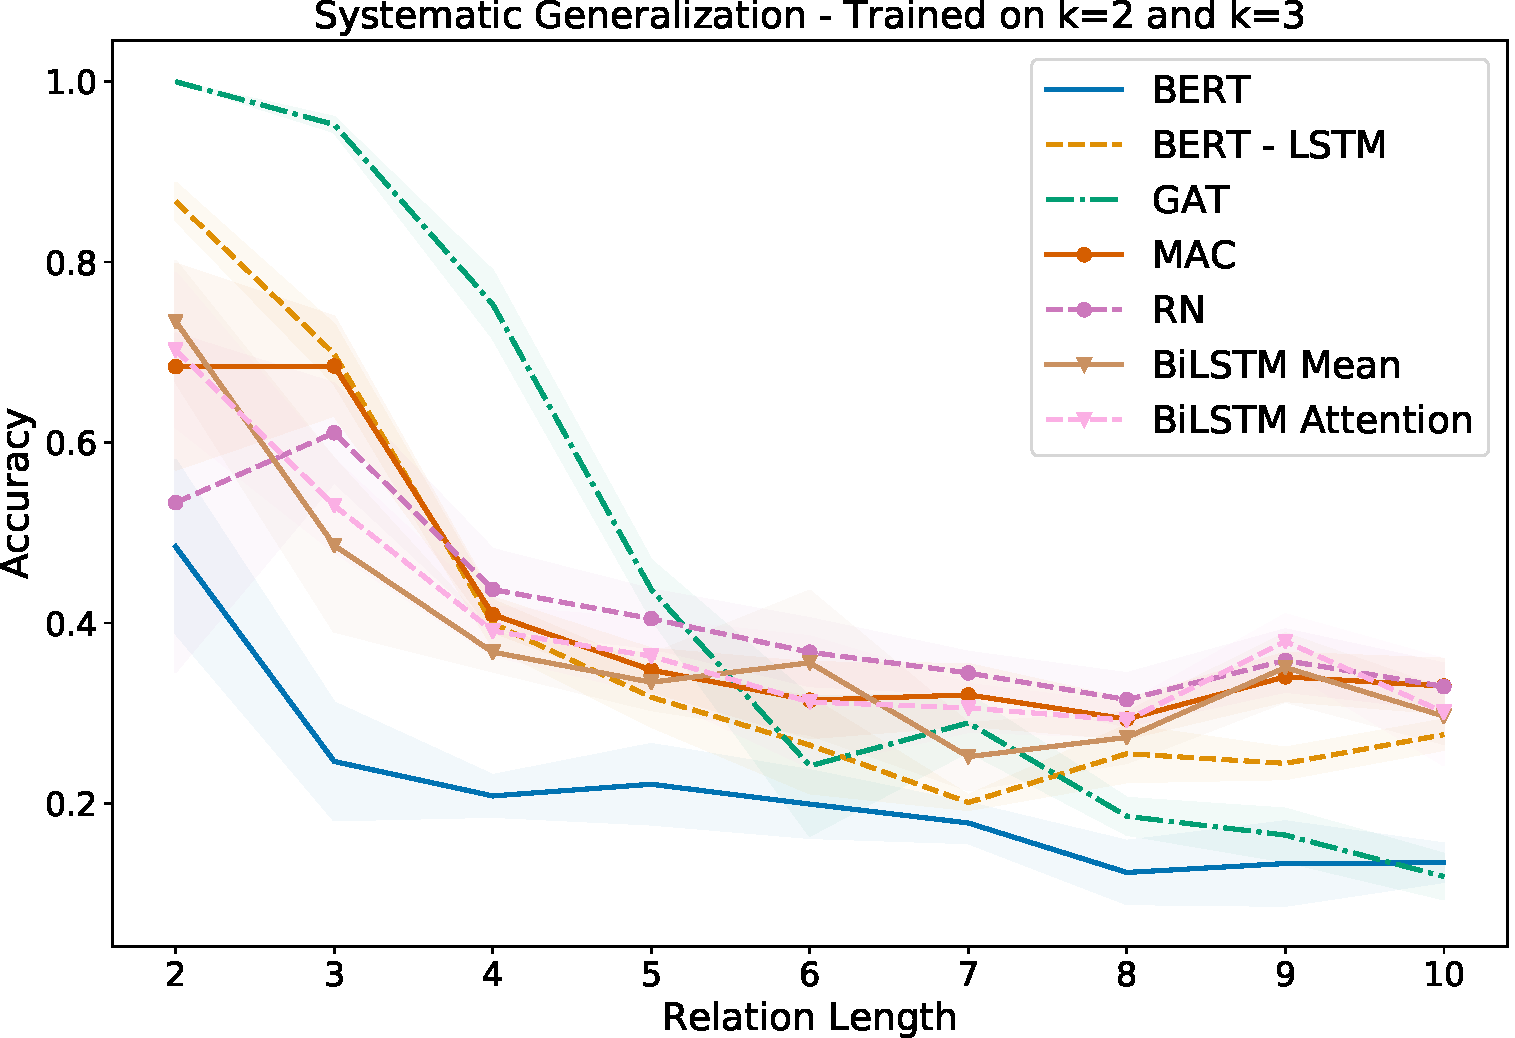
\includegraphics[width=0.48\textwidth]{figs/clutrr/emnlp/sys_gen_23.pdf} }}%
    \qquad
    \hspace{-20pt}
    \subfloat{{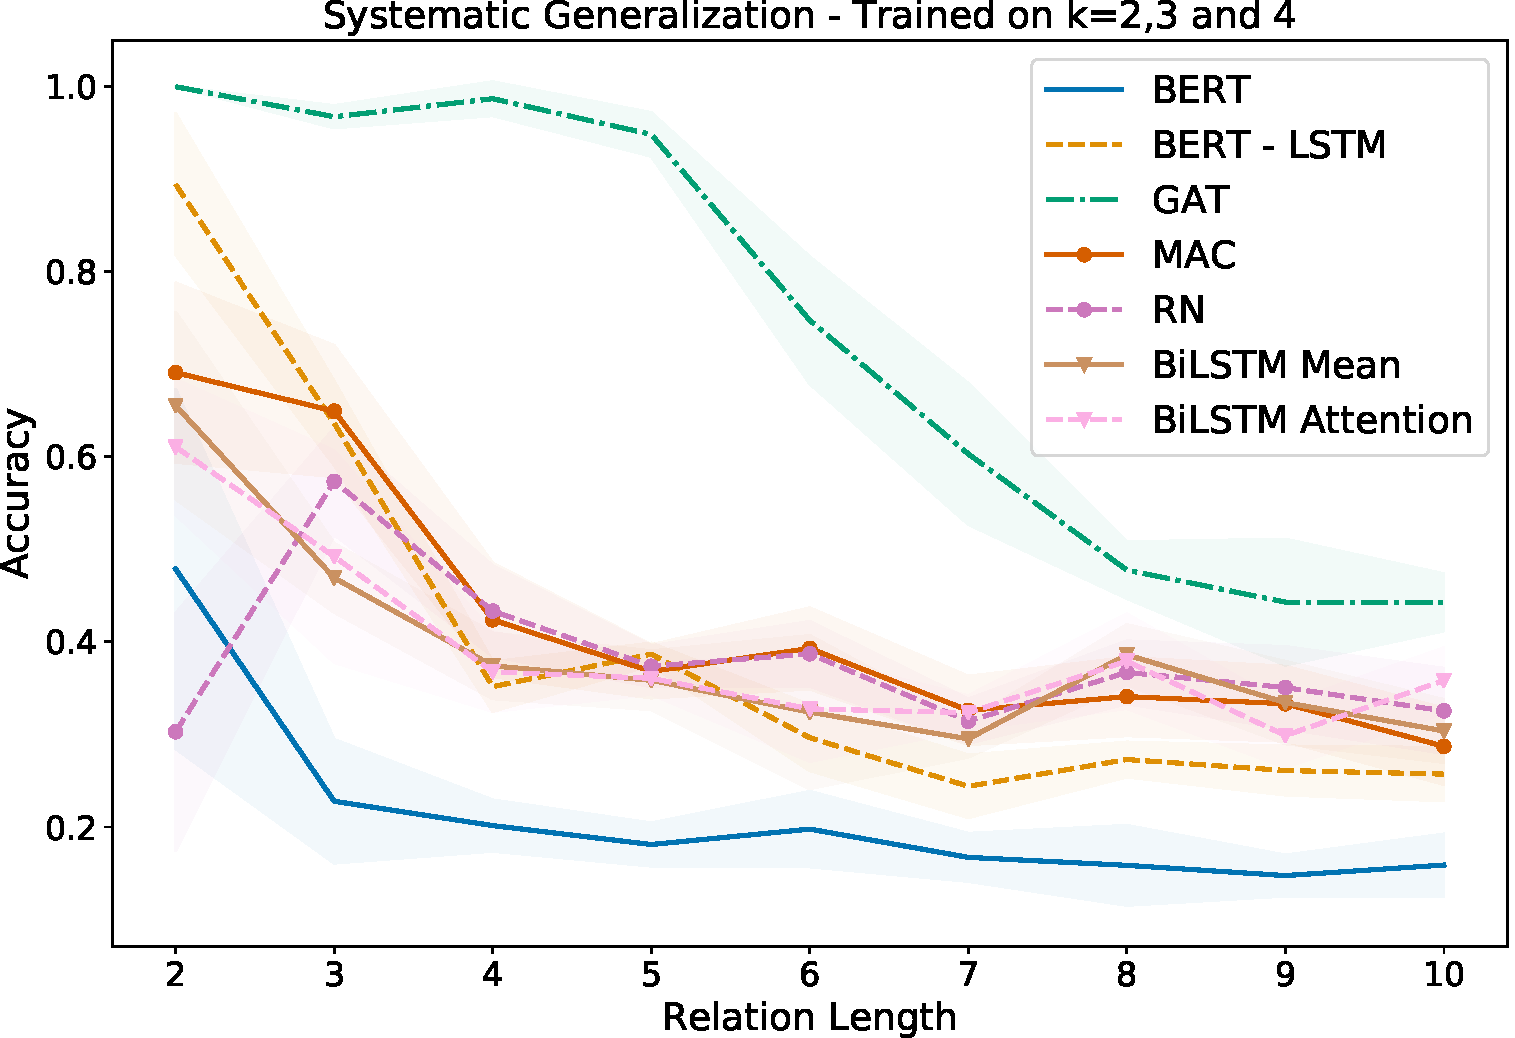
\includegraphics[width=0.48\textwidth]{figs/clutrr/emnlp/sys_gen_234.pdf} }}%
    \caption{Systematic generalization performance of different models when trained on clauses of length $k=2,3$ (Left) and $k=2,3,4$ (Right).}
    \label{fig:gen_1}
\end{figure*}



\subsection{The benefit of structure}
\label{sec:clutrr_structure}

The empirical results on systematic generalization also provide insight into how the text-based \acrshort{nlu} systems compare against the graph-based GAT model that has full access to the logical graph structure underlying the stories (\textbf{Q2}).
Indeed, the relatively strong performance of the GAT model (Figure \ref{fig:gen_1}) suggests that the language-based models fail to learn a robust mapping from the natural language narratives to the underlying logical facts.

\begin{figure*}[!ht]
     \centering
    \subfloat{{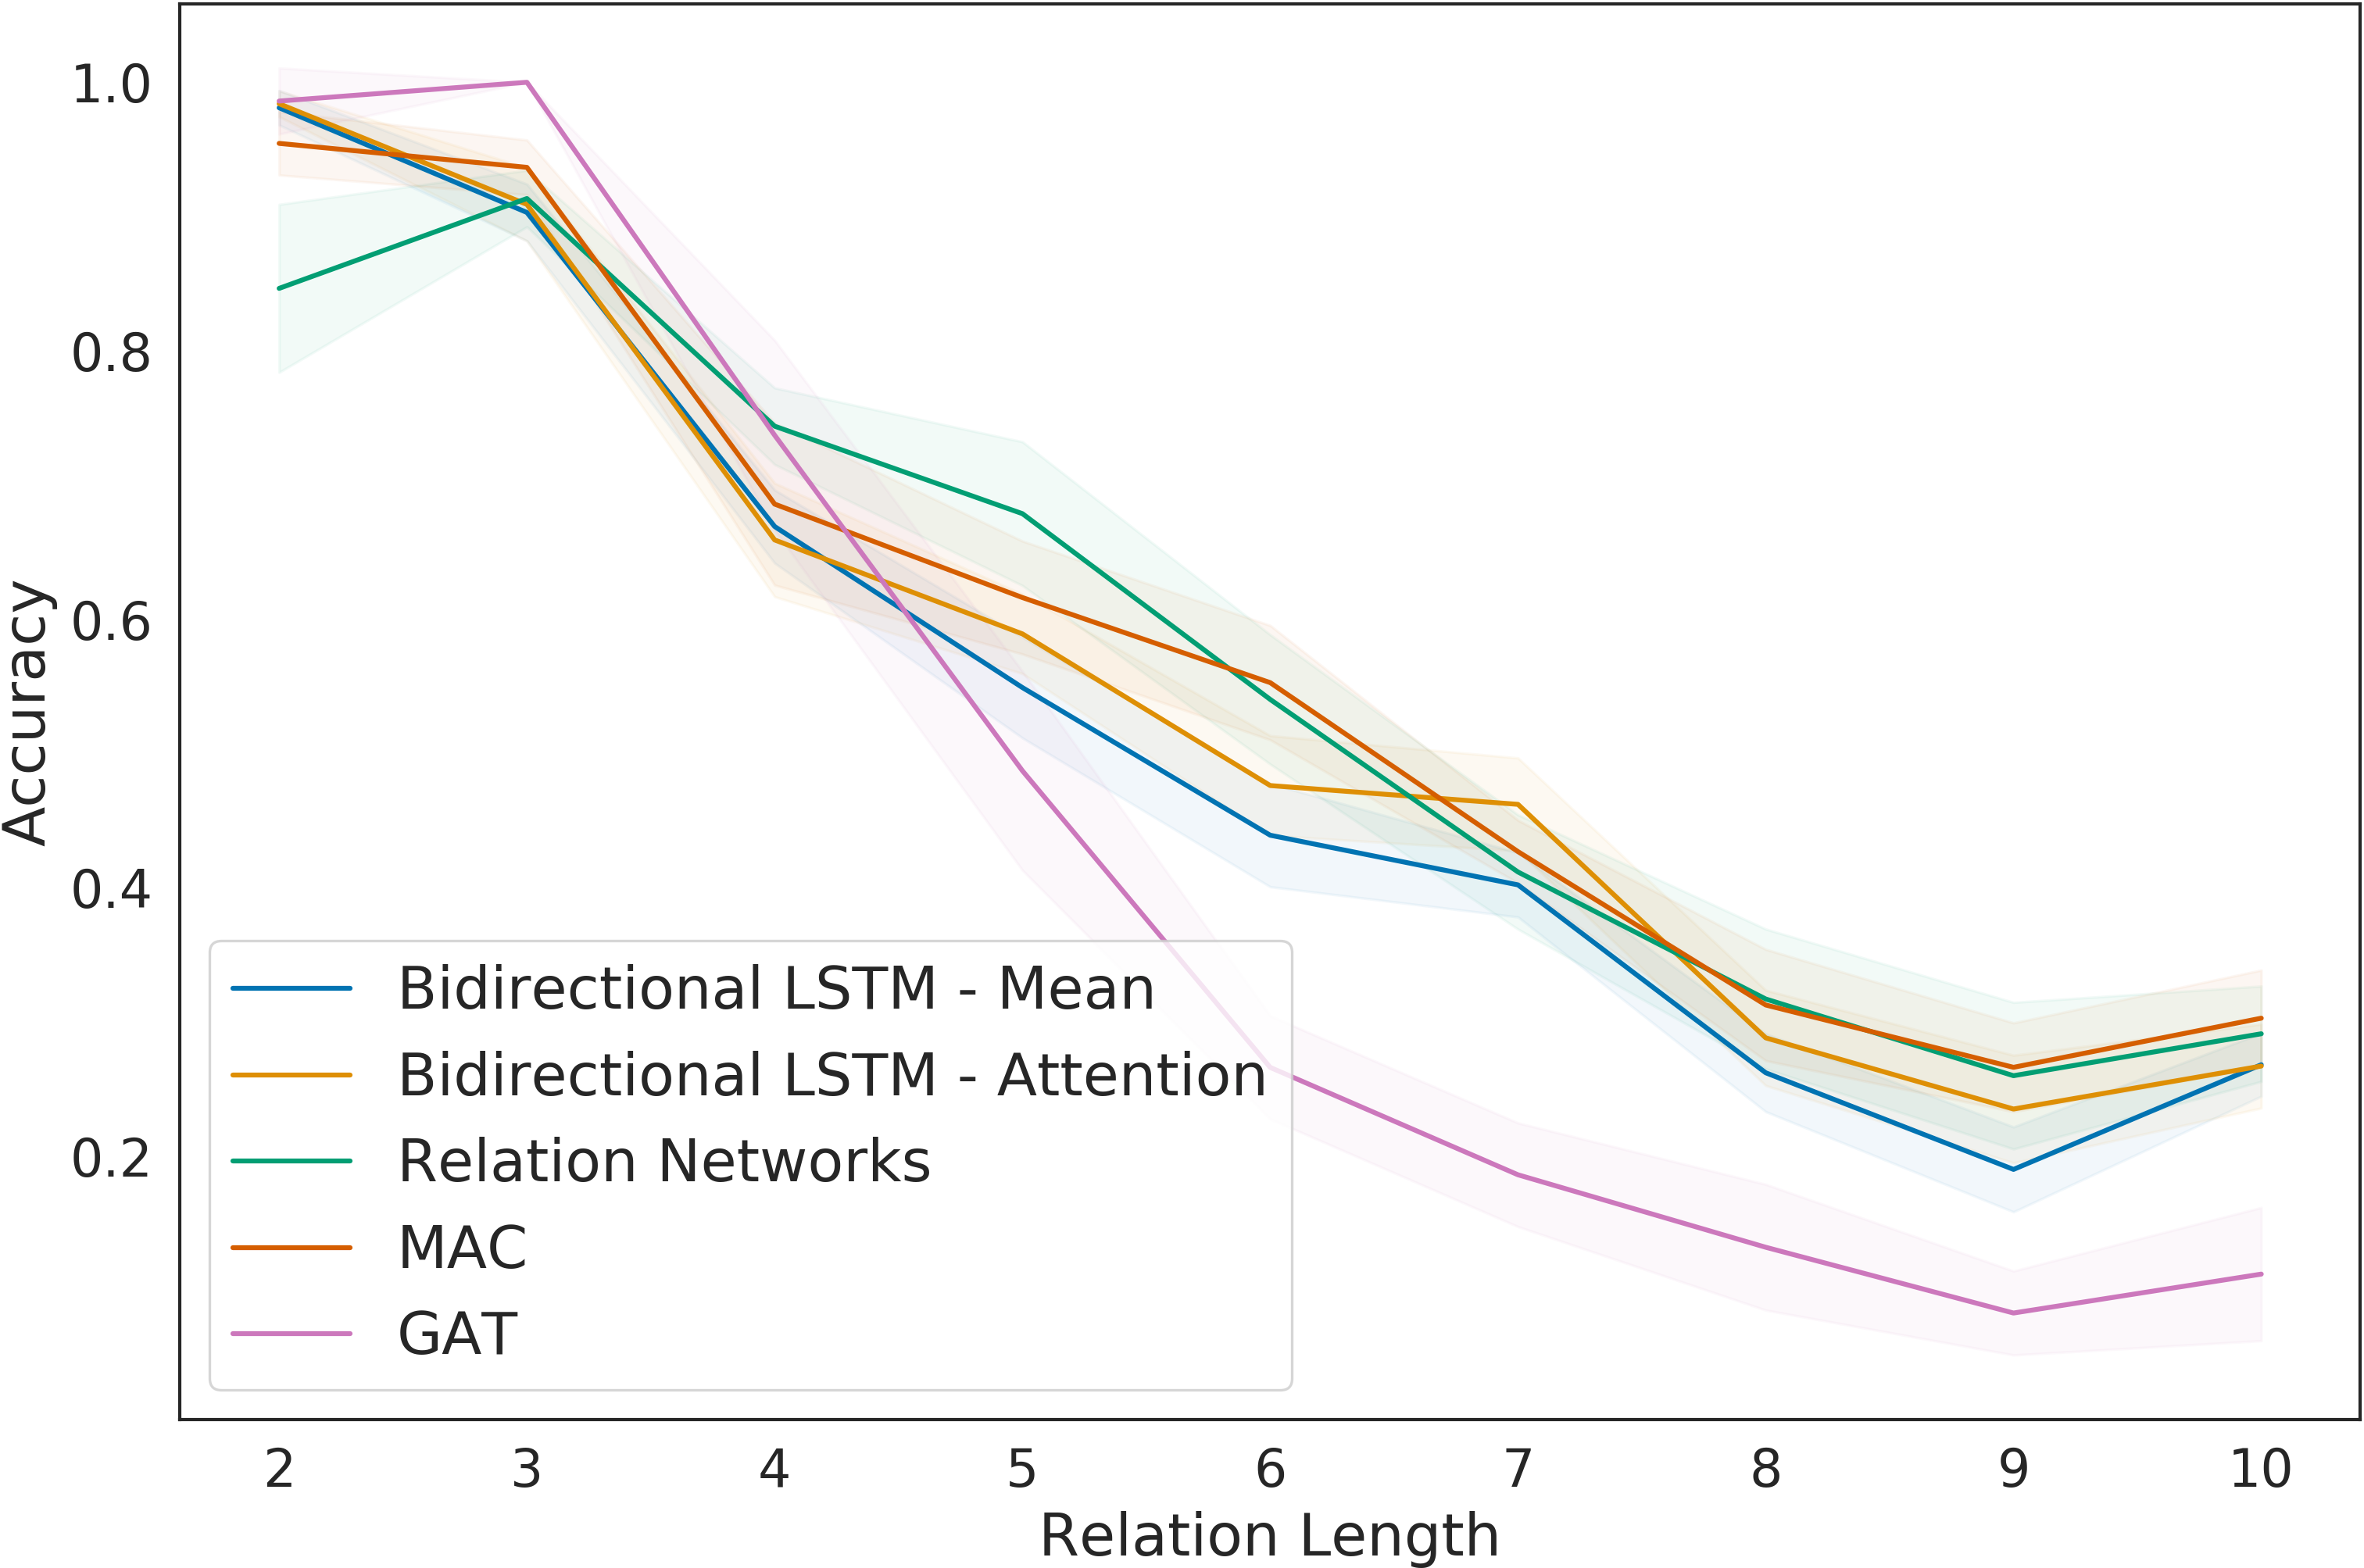
\includegraphics[width=0.48\textwidth]{figs/clutrr/sys_gen_amt_23.png} }}%
    \qquad
    \hspace{-20pt}
    \subfloat{{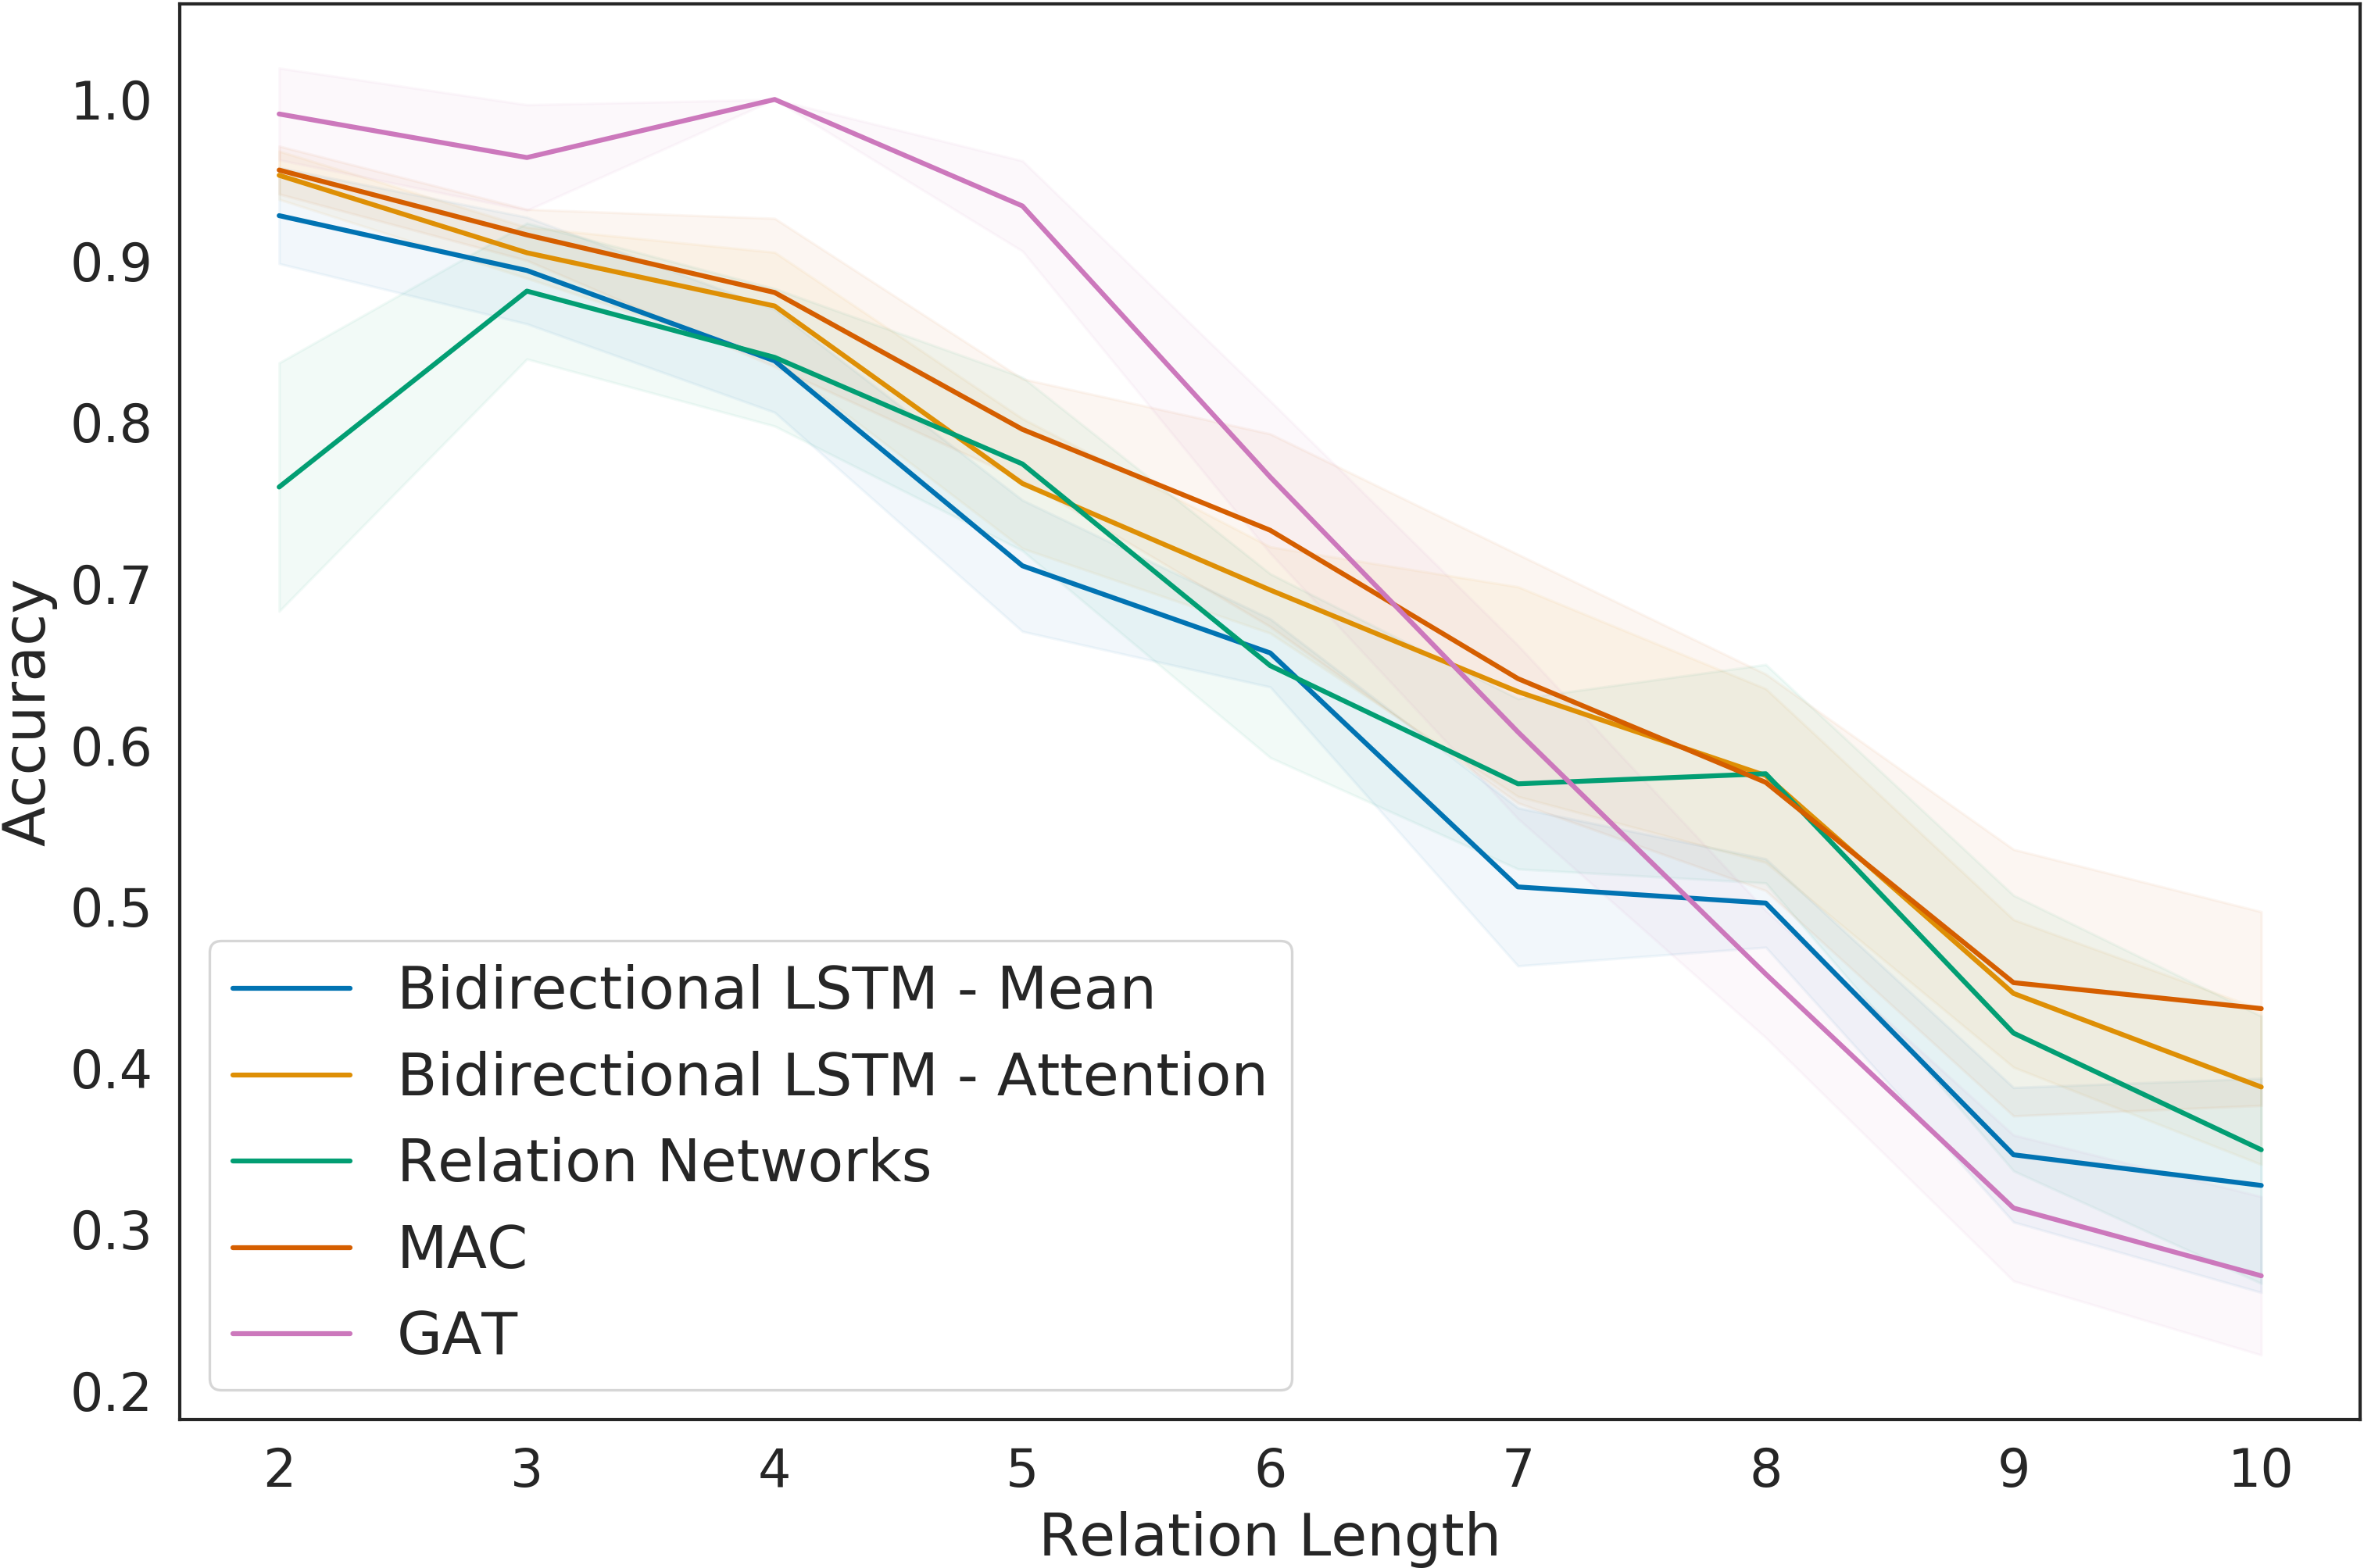
\includegraphics[width=0.48\textwidth]{figs/clutrr/sys_gen_amt_234.png} }}%
    \caption{Systematic Generalizability of different models on \texttt{CLUTRR-Gen} task (having 20\% less placeholders and without training and testing placeholder split), when {\bf Left:} trained with $k=2$ and $k=3$ and {\bf Right:} trained with $k=2,3$ and $4$}%
    \label{fig:gen_app_1}
\end{figure*}



To further confirm this trend, we ran experiments with modified train and test splits for the text-based models, where the same set of natural language paraphrases were used to construct the narratives in both the train and test splits (\autoref{fig:gen_app_1}). In this simplified setting, the text-based models must still learn to reason about held-out logical patterns, but the difficulty of parsing the natural language is essentially removed, as the same natural language paraphrases are used during testing and training. We found that the text-based models were competitive with the GAT model in this simplified setting, confirming that the poor performance of the text-based models on the main task is driven by the difficulty of parsing the unseen natural language narratives.

\subsection{Robust Reasoning}
\label{sec:clutrr_robust_reasoning}

\begin{table*}[t!]
\resizebox{\textwidth}{!}{
% Please add the following required packages to your document preamble:
% \usepackage{multirow}
\begin{tabular}{@{}cccccccc|c@{}}
\toprule
\multicolumn{1}{l}{} & \multicolumn{1}{l}{Models} & \multicolumn{6}{c}{Unstructured models (no graph)} & \multicolumn{1}{l}{Structured model (with graph)} \\ \midrule
\multicolumn{1}{l}{Training} & \multicolumn{1}{l|}{Testing} & BiLSTM - Attention & BiLSTM - Mean & RN & MAC & \multicolumn{1}{l}{BERT} & \multicolumn{1}{l|}{BERT-LSTM} & GAT \\ \midrule
Clean & \multicolumn{1}{c|}{Clean} & 0.58 \tiny $\pm 0.05$ & 0.53 \tiny $\pm 0.05$ & 0.49 \tiny $\pm 0.06$ & 0.63 \tiny $\pm 0.08$ & 0.37 \tiny $\pm 0.06$ & 0.67 \tiny $\pm 0.03$ & \textbf{1.0} \tiny $\pm 0.0$ \\ 
 & \multicolumn{1}{c|}{Supporting} & \textbf{0.76} \tiny $\pm 0.02$ & 0.64 \tiny $\pm 0.22$ & 0.58 \tiny $\pm 0.06$ & 0.71 \tiny $\pm 0.07$ & 0.28 \tiny $\pm 0.1$ & 0.66 \tiny $\pm 0.06$ & 0.24 \tiny $\pm 0.2$ \\
 & \multicolumn{1}{c|}{Irrelevant} & 0.7 \tiny $\pm 0.15$ & \textbf{0.76} \tiny $\pm 0.02$ & 0.59 \tiny $\pm 0.06$ & 0.69 \tiny $\pm 0.05$ & 0.24 \tiny $\pm 0.08$ & 0.55 \tiny $\pm 0.03$ & 0.51 \tiny $\pm 0.15$ \\
 & \multicolumn{1}{c|}{Disconnected} & 0.49 \tiny $\pm 0.05$ & 0.45 \tiny $\pm 0.05$ & 0.5 \tiny $\pm 0.06$ & 0.59 \tiny $\pm 0.05$ & 0.24 \tiny $\pm 0.08$ & 0.5 \tiny $\pm 0.06$ & \textbf{0.8} \tiny $\pm 0.17$ \\ \midrule
Supporting & \multicolumn{1}{c|}{Supporting} & 0.67 \tiny $\pm 0.06$ & 0.66 \tiny $\pm 0.07$ & 0.68 \tiny $\pm 0.05$ & 0.65 \tiny $\pm 0.04$ & 0.32 \tiny $\pm 0.09$ & 0.57 \tiny $\pm 0.04$ & \textbf{0.98} \tiny $\pm 0.01$ \\
\midrule
Irrelevant & \multicolumn{1}{c|}{Irrelevant} & 0.51 \tiny $\pm 0.06$ & 0.52 \tiny $\pm 0.06$ & 0.5 \tiny $\pm 0.04$ & 0.56 \tiny $\pm 0.04$ & 0.25 \tiny $\pm 0.06$ & 0.53 \tiny $\pm 0.06$ & \textbf{0.93} \tiny $\pm 0.01$ \\
\midrule
Disconnected & \multicolumn{1}{c|}{Disconnected} & 0.57 \tiny $\pm 0.07$ & 0.57 \tiny $\pm 0.06$ & 0.45 \tiny $\pm 0.11$ & 0.4 \tiny $\pm 0.1$ & 0.17 \tiny $\pm 0.05$ & 0.47 \tiny $\pm 0.06$ & \textbf{0.96} \tiny $\pm 0.01$ \\ \midrule
\multicolumn{1}{l}{Average} & \multicolumn{1}{c|}{} & \textbf{0.61} \tiny $\pm 0.08$ & 0.59 \tiny $\pm 0.08$ & 0.54 \tiny $\pm 0.07$ & \textbf{0.61} \tiny $\pm 0.06$ & 0.30 \tiny $\pm 0.07$ & 0.56 \tiny $\pm 0.05$ & \textbf{0.77} \tiny $\pm 0.09$ \\ \bottomrule
\end{tabular}}
\caption{Testing the robustness of the various models when training and testing on stories containing various types of noise facts. The types of noise facts (supporting, irrelevant, and disconnected) are defined in Section .}
\label{tab:robust}
\end{table*}


Finally, we use CLUTRR to systematically evaluate how various baseline neural language understanding systems cope with noise (\textbf{Q3}).
In all the experiments we provide a combination of $k=2$ and $k=3$ length clauses in training and testing, with noise facts being added to the train and/or test set depending on the setting (Table \ref{tab:robust}).
We use the different types of noise facts defined in Section \ref{sec:clutrr_robust_data}..

Overall, we find that the GAT baseline outperforms the unstructured text-based models across most testing scenarios (Table \ref{tab:robust}), which showcases the benefit of a structured feature space for robust reasoning.
When training on clean data and testing on noisy data, we observe two interesting trends that highlight the benefits and shortcomings of the various model classes:
\begin{enumerate}[leftmargin=*, topsep=2pt, itemsep=0pt]
    \item All the text-based models excluding BERT actually perform better when testing on examples that have {\em supporting} or {\em irrelevant} facts added. This suggests that these models actually benefit from having more content related to the entities in the story. Even though this content is not strictly useful or needed for the reasoning task, it may provide some linguistic cues (e.g., about entity genders) that the models exploit. In contrast, the BERT-based models do not benefit from the inclusion of this extra content, which is perhaps due to the fact that they are already built upon a strong language model (e.g., that already adequately captures entity genders.)
    \item  The GAT model performs poorly when {\em supporting} facts are added but has no performance drop when {\em disconnected} facts are added. This suggests that the GAT model is sensitive to changes that introduce cycles in the underlying graph structure but is robust to the addition of noise that is disconnected from the target entities.
\end{enumerate}

\subsubsection{Learning from noisy data}

Moreover, when we trained on noisy examples, we found that only the GAT model was able to consistently improve its performance (Table \ref{tab:robust}).
We notice that the GAT model, having access to the true underlying graph of the puzzles, perform better across different testing scenarios when trained with the noisy data. As the \textit{Supporting facts} contains cycles, it is difficult for GAT to generalize for a dataset with cycles when it is trained on a dataset without cycles. However, when trained with cycles, GAT learns to attend to \textit{all} the paths leading to the correct answer. This effect is disastrous when GAT is tested on \textit{Irrelevant facts} which contains dangling paths as GAT still tries to attend to all the paths. Training on \textit{Irrelevant facts} proved to be most beneficial to GAT, as the model now perfectly attends to \textit{only relevant paths}.
Since \textit{Disconnected facts} contains disconnected paths, the message passing function of the graph is unable to forward any information from the disjoint cliques, thereby having superior testing scores throughout several scenarios.

\begin{table*}[t!]
\resizebox{\textwidth}{!}{
% Please add the following required packages to your document preamble:
% \usepackage{multirow}
\begin{tabular}{@{}cccccccc|c@{}}
\toprule
\multicolumn{1}{l}{} & \multicolumn{1}{l}{Models} & \multicolumn{6}{c}{Unstructured models (no graph)} & \multicolumn{1}{l}{Structured model (with graph)} \\ \midrule
\multicolumn{1}{l|}{Training} & \multicolumn{1}{l|}{Testing} & BiLSTM - Attention & BiLSTM - Mean & RN & MAC & \multicolumn{1}{l}{BERT} & \multicolumn{1}{l|}{BERT-LSTM} & GAT \\ \midrule
Supporting & \multicolumn{1}{c|}{Clean} & 0.38 \tiny $\pm 0.04$ & 0.32 \tiny $\pm 0.04$ & 0.4 \tiny $\pm 0.09$ & 0.45 \tiny $\pm 0.03$ & 0.19 \tiny $\pm 0.06$ & 0.39 \tiny $\pm 0.06$ & \textbf{0.92} \tiny $\pm 0.17$ \\
\multicolumn{1}{l}{} & \multicolumn{1}{c|}{Supporting} & 0.67 \tiny $\pm 0.06$ & 0.66 \tiny $\pm 0.07$ & 0.68 \tiny $\pm 0.05$ & 0.65 \tiny $\pm 0.04$ & 0.32 \tiny $\pm 0.09$ & 0.57 \tiny $\pm 0.04$ & \textbf{0.98} \tiny $\pm 0.01$ \\
 & \multicolumn{1}{c|}{Irrelevant} & 0.44 \tiny $\pm 0.03$ & 0.39 \tiny $\pm 0.03$ & \textbf{0.51} \tiny $\pm 0.08$ & 0.46 \tiny $\pm 0.09$ & 0.2 \tiny $\pm 0.06$ & 0.36 \tiny $\pm 0.05$ & 0.5 \tiny $\pm 0.23$ \\
 & \multicolumn{1}{c|}{Disconnected} & 0.31 \tiny $\pm 0.21$ & 0.25 \tiny $\pm 0.16$ & 0.47 \tiny $\pm 0.08$ & 0.41 \tiny $\pm 0.06$ & 0.2 \tiny $\pm 0.08$ & 0.32 \tiny $\pm 0.04$ & \textbf{0.92} \tiny $\pm 0.05$ \\ \midrule
Irrelevant & \multicolumn{1}{c|}{Clean} & 0.57 \tiny $\pm 0.05$ & 0.56 \tiny $\pm 0.05$ & 0.46 \tiny $\pm 0.13$ & 0.67 \tiny $\pm 0.05$ & 0.24 \tiny $\pm 0.06$ & 0.46 \tiny $\pm 0.08$ & \textbf{0.92} \tiny $\pm 0.0$ \\
 & \multicolumn{1}{c|}{Supporting} & 0.38 \tiny $\pm 0.22$ & 0.31 \tiny $\pm 0.16$ & 0.61 \tiny $\pm 0.07$ & 0.61 \tiny $\pm 0.04$ & 0.27 \tiny $\pm 0.06$ & 0.46 \tiny $\pm 0.04$ & \textbf{0.77} \tiny $\pm 0.12$ \\
\multicolumn{1}{l}{} & \multicolumn{1}{c|}{Irrelevant} & 0.51 \tiny $\pm 0.06$ & 0.52 \tiny $\pm 0.06$ & 0.5 \tiny $\pm 0.04$ & 0.56 \tiny $\pm 0.04$ & 0.25 \tiny $\pm 0.06$ & 0.53 \tiny $\pm 0.06$ & \textbf{0.93} \tiny $\pm 0.01$ \\
 & \multicolumn{1}{c|}{Disconnected} & 0.44 \tiny $\pm 0.26$ & 0.54 \tiny $\pm 0.27$ & 0.55 \tiny $\pm 0.05$ & 0.61 \tiny $\pm 0.06$ & 0.26 \tiny $\pm 0.03$ & 0.45 \tiny $\pm 0.08$ & \textbf{0.85} \tiny $\pm 0.25$ \\ \midrule
\multirow{3}{*}{Disconnected} & \multicolumn{1}{c|}{Clean} & 0.45 \tiny $\pm 0.02$ & 0.47 \tiny $\pm 0.03$ & 0.53 \tiny $\pm 0.09$ & 0.5 \tiny $\pm 0.06$ & 0.22 \tiny $\pm 0.09$ & 0.44 \tiny $\pm 0.05$ & \textbf{0.75} \tiny $\pm 0.07$ \\
 & \multicolumn{1}{c|}{Supporting} & 0.47 \tiny $\pm 0.03$ & 0.46 \tiny $\pm 0.05$ & 0.54 \tiny $\pm 0.03$ & 0.58 \tiny $\pm 0.06$ & 0.22 \tiny $\pm 0.06$ & 0.38 \tiny $\pm 0.08$ & \textbf{0.78} \tiny $\pm 0.12$ \\
 & \multicolumn{1}{c|}{Irrelevant} & 0.47 \tiny $\pm 0.05$ & 0.48 \tiny $\pm 0.03$ & 0.52 \tiny $\pm 0.04$ & 0.51 \tiny $\pm 0.05$ & 0.17 \tiny $\pm 0.04$ & 0.38 \tiny $\pm 0.05$ & \textbf{0.56} \tiny $\pm 0.26$ \\
\multicolumn{1}{l}{} & \multicolumn{1}{c|}{Disconnected} & 0.57 \tiny $\pm 0.07$ & 0.57 \tiny $\pm 0.06$ & 0.45 \tiny $\pm 0.11$ & 0.4 \tiny $\pm 0.1$ & 0.17 \tiny $\pm 0.05$ & 0.47 \tiny $\pm 0.06$ & \textbf{0.96} \tiny $\pm 0.01$ \\ \midrule
\multicolumn{1}{l}{Average} & \multicolumn{1}{c|}{} & 0.47 \tiny $\pm 0.08$ & 0.46 \tiny $\pm 0.08$ & 0.52 \tiny $\pm 0.07$ & \textbf{0.53} \tiny $\pm 0.06$ & 0.23 \tiny $\pm 0.07$ & 0.43 \tiny $\pm 0.05$ & \textbf{0.82} \tiny $\pm 0.09$ \\ \bottomrule
\end{tabular}}
\caption{Testing the robustness of the various models when trained various types of noisy facts and evaluated on other noisy / clean facts.}
\label{tab:robust_appen}
\end{table*}


Again, these results highlights the performance gap between the unstructured text-based models and GAT for solving the CLUTRR task.

\subsubsection{Learning with synthetic placeholders}

In order to further understand the effect of language placeholders on robustness, we performed another set of experiments where we use bABI \cite{Weston2015-is} style simple placeholders (Table \ref{tab:robust_toy_appen}). We observe a marked increase in performance of all \acrshort{nlu} models, where they significantly decrease the gap between their performance with that of GAT, even outperforming GAT on various settings. This shows the significance of using paraphrased placeholders in devising the complexity of the dataset.

\begin{table*}[t!]
\resizebox{\textwidth}{!}{
% Please add the following required packages to your document preamble:
% \usepackage{multirow}
\begin{tabular}{@{}cccccccc|c@{}}
\toprule
\multicolumn{1}{l}{} & \multicolumn{1}{l}{Models} & \multicolumn{6}{c}{Unstructured models (no graph)} & \multicolumn{1}{l}{Structured model (with graph)} \\ \midrule
\multicolumn{1}{l|}{Training} & \multicolumn{1}{l|}{Testing} & BiLSTM - Attention & BiLSTM - Mean & RN & MAC & \multicolumn{1}{l}{BERT} & \multicolumn{1}{l|}{BERT-LSTM} & GAT \\ \midrule
Supporting & \multicolumn{1}{c|}{Clean} & 0.96 \tiny $\pm 0.01$ & \textbf{0.97} \tiny $\pm 0.01$ & 0.88 \tiny $\pm 0.05$ & 0.94 \tiny $\pm 0.02$ & 0.48 \tiny $\pm 0.08$ & 0.57 \tiny $\pm 0.08$ & 0.92 \tiny $\pm 0.17$ \\
\multicolumn{1}{l}{} & \multicolumn{1}{c|}{Supporting} & 0.96 \tiny $\pm 0.03$ & 0.96 \tiny $\pm 0.03$ & 0.97 \tiny $\pm 0.01$ & 0.97 \tiny $\pm 0.01$ & 0.75 \tiny $\pm 0.07$ & 0.88 \tiny $\pm 0.05$ & \textbf{0.98} \tiny $\pm 0.01$ \\
 & \multicolumn{1}{c|}{Irrelevant} & 0.92 \tiny $\pm 0.02$ & \textbf{0.93} \tiny $\pm 0.01$ & 0.9 \tiny $\pm 0.03$ & 0.91 \tiny $\pm 0.01$ & 0.56 \tiny $\pm 0.04$ & 0.54 \tiny $\pm 0.06$ & 0.5 \tiny $\pm 0.23$ \\
 & \multicolumn{1}{c|}{Disconnected} & 0.8 \tiny $\pm 0.04$ & 0.83 \tiny $\pm 0.04$ & 0.76 \tiny $\pm 0.08$ & 0.86 \tiny $\pm 0.04$ & 0.27 \tiny $\pm 0.06$ & 0.42 \tiny $\pm 0.08$ & \textbf{0.92} \tiny $\pm 0.05$ \\ \midrule
Irrelevant & \multicolumn{1}{c|}{Clean} & 0.63 \tiny $\pm 0.02$ & 0.61 \tiny $\pm 0.07$ & 0.85 \tiny $\pm 0.09$ & 0.8 \tiny $\pm 0.07$ & 0.53 \tiny $\pm 0.09$ & 0.44 \tiny $\pm 0.06$ & \textbf{0.92} \tiny $\pm 0.0$ \\
 & \multicolumn{1}{c|}{Supporting} & 0.66 \tiny $\pm 0.03$ & 0.64 \tiny $\pm 0.04$ & 0.69 \tiny $\pm 0.06$ & 0.76 \tiny $\pm 0.06$ & 0.42 \tiny $\pm 0.08$ & 0.43 \tiny $\pm 0.08$ & \textbf{0.77} \tiny $\pm 0.12$ \\
\multicolumn{1}{l}{} & \multicolumn{1}{c|}{Irrelevant} & 0.89 \tiny $\pm 0.04$ & 0.86 \tiny $\pm 0.1$ & 0.74 \tiny $\pm 0.11$ & 0.78 \tiny $\pm 0.06$ & 0.61 \tiny $\pm 0.1$ & 0.83 \tiny $\pm 0.06$ & \textbf{0.93} \tiny $\pm 0.01$ \\
 & \multicolumn{1}{c|}{Disconnected} & 0.64 \tiny $\pm 0.02$ & 0.62 \tiny $\pm 0.05$ & 0.72 \tiny $\pm 0.05$ & 0.73 \tiny $\pm 0.04$ & 0.41 \tiny $\pm 0.04$ & 0.61 \tiny $\pm 0.05$ & \textbf{0.85} \tiny $\pm 0.25$ \\ \midrule
\multirow{3}{*}{Disconnected} & \multicolumn{1}{c|}{Clean} & 0.9 \tiny $\pm 0.05$ & 0.82 \tiny $\pm 0.12$ & \textbf{0.94} \tiny $\pm 0.02$ & 0.93 \tiny $\pm 0.04$ & 0.68 \tiny $\pm 0.07$ & 0.64 \tiny $\pm 0.02$ & 0.75 \tiny $\pm 0.07$ \\
 & \multicolumn{1}{c|}{Supporting} & 0.87 \tiny $\pm 0.04$ & 0.82 \tiny $\pm 0.05$ & 0.85 \tiny $\pm 0.03$ & \textbf{0.88} \tiny $\pm 0.04$ & 0.54 \tiny $\pm 0.08$ & 0.5 \tiny $\pm 0.05$ & 0.78 \tiny $\pm 0.12$ \\
 & \multicolumn{1}{c|}{Irrelevant} & \textbf{0.87} \tiny $\pm 0.03$ & 0.85 \tiny $\pm 0.03$ & 0.83 \tiny $\pm 0.03$ & 0.87 \tiny $\pm 0.02$ & 0.59 \tiny $\pm 0.09$ & 0.58 \tiny $\pm 0.09$ & 0.56 \tiny $\pm 0.26$ \\
\multicolumn{1}{l}{} & \multicolumn{1}{c|}{Disconnected} & 0.91 \tiny $\pm 0.04$ & 0.91 \tiny $\pm 0.03$ & 0.8 \tiny $\pm 0.17$ & 0.71 \tiny $\pm 0.11$ & 0.49 \tiny $\pm 0.1$ & 0.79 \tiny $\pm 0.1$ & \textbf{0.96} \tiny $\pm 0.01$ \\ \midrule
\multicolumn{1}{l}{Average} & \multicolumn{1}{c|}{} & 0.83 \tiny $\pm 0.08$ & 0.82 \tiny $\pm 0.08$ & 0.83 \tiny $\pm 0.07$ & \textbf{0.84} \tiny $\pm 0.06$ & 0.58 \tiny $\pm 0.07$ & 0.60 \tiny $\pm 0.05$ & \textbf{0.82} \tiny $\pm 0.09$ \\ \bottomrule
\end{tabular}}
\caption{Testing the robustness on toy placeholders of the various models when trained various types of noisy facts and evaluated on other noisy / clean facts.}
\label{tab:robust_toy_appen}
\end{table*}






% TODO insert figure
% \begin{center}
% 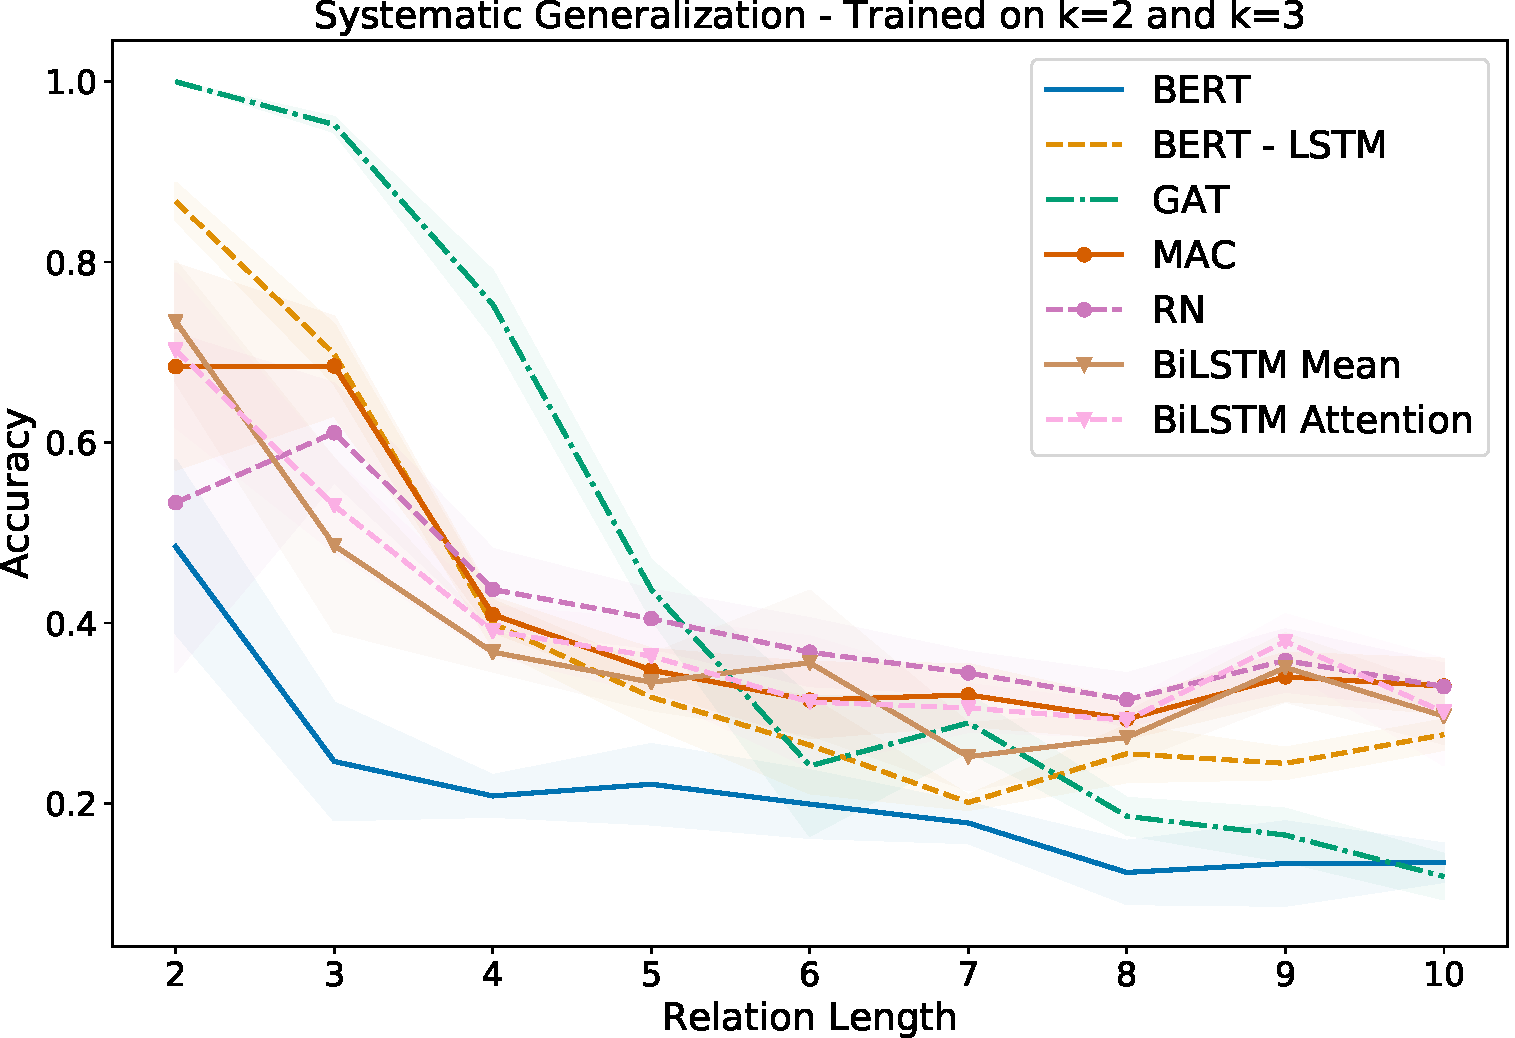
\includegraphics[height=0.3\textwidth]{figs/clutrr/emnlp/sys_gen_23.pdf}
% 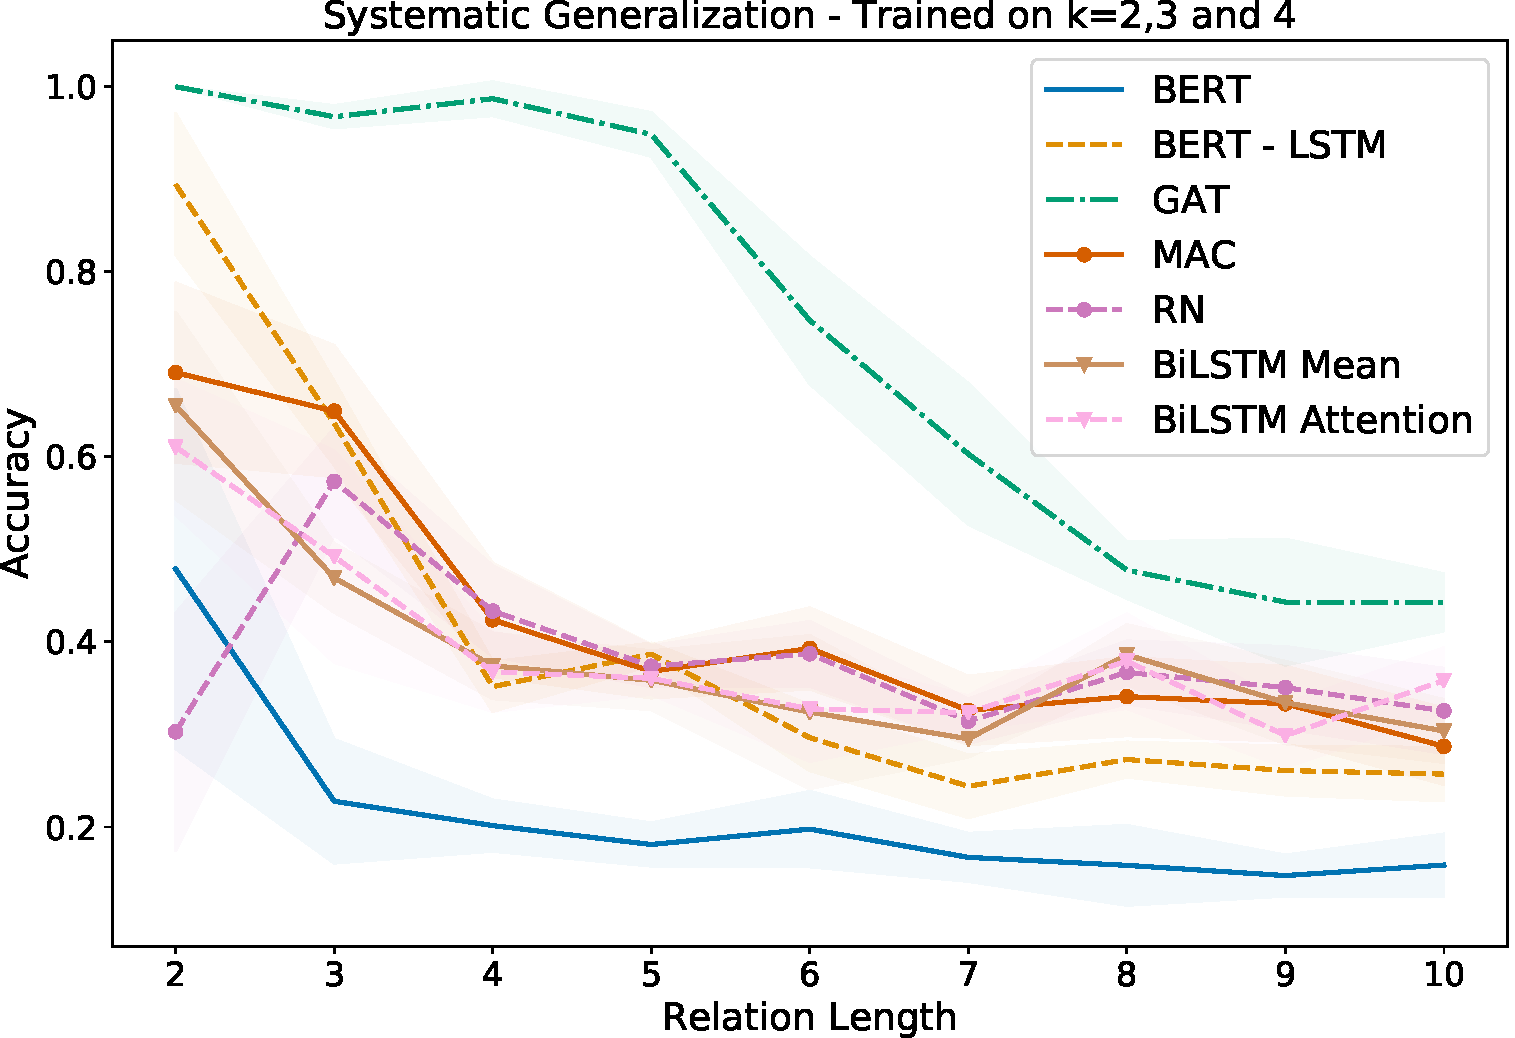
\includegraphics[height=0.3\textwidth]{figs/clutrr/emnlp/sys_gen_234.pdf}
% \end{center}
% \begin{figure}[htbp]
% \centering
% 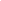
\includegraphics[height=0.0001in]{figs/empy_fig.png}
% \caption{Systematic generalization when train on k=\(2\) and \(3\).}
% \end{figure}


\section{Related Work}
\label{sec:clutrr_related_work}

To design the CLUTRR dataset, we draw inspiration from the classic work on inductive logic programming (ILP), a long line of reading comprehension benchmarks in NLP, as well as work combining language and knowledge graphs.

\subsection{Reading comprehension benchmarks}

Many datasets have been proposed to test the reading comprehension ability of NLP systems. This includes the SQuAD \citep{rajpurkar-etal-2016-squad}, NewsQA \citep{Trischler2016-fc}, and MCTest \citep{richardson2013mctest} benchmarks that focus on factual questions; the SNLI \citep{bowman-etal-2015-large} and MultiNLI \citep{williams-etal-2018-broad} benchmarks for sentence understanding; and the bABI tasks \citep{Weston2015-is}, to name a few.
Our primary contribution to this line of work is the development of a carefully designed {\em diagnostic} benchmark to evaluate model robustness and systematic generalization in the context of \acrshort{nlu}.

\subsection{Systematic generalization}

A growing body of literature has demonstrated that \acrshort{nlu} models tend to exploit statistical artifacts in datasets and lack true generalization capabilities \citep{jia-liang-2017-adversarial,gururangan-etal-2018-annotation, kaushik2018much,Lake2018:SCAN}.
These critical examinations have dovetailed with similar studies on visual question answering \citep{agrawal2016analyzing,bahdanau2018systematic,Johnson2016-mw}.
CLUTRR, contributes to this growing area by introducing a principled and flexible benchmark to evaluate systematic generalization in the context of language understanding---with our notion of systematic generalization being grounded in classic work on inductive logic programming (ILP) \cite{Quinlan1990-iv}.


\subsection{Question-answering with knowledge graphs}

Our work is also related to the domain of question answering and reasoning in knowledge graphs \citep{das2017go, xiong2018one, NIPS2018_7473, 8587330, xiong2017deeppath, welbl2018constructing, kartsaklis2018mapping}, where either the model is provided with a knowledge graph to perform inference over or where the model must infer a knowledge graph from the text itself.
However, unlike previous benchmarks in this domain---which are generally {\em transductive} and focus on leveraging and extracting knowledge graphs as a source of background knowledge about a fixed set of entities---CLUTRR requires {\em inductive logical reasoning}, where every example requires reasoning over a new set of previously unseen entities.


\section{Discussion}
\label{sec:clutrr_discussion}

In this paper we introduced the CLUTRR benchmark suite to test the systematic generalization and inductive reasoning capabilities of \acrshort{nlu} systems.
We demonstrated the diagnostic capabilities of CLUTRR and found that existing \acrshort{nlu} systems exhibit relatively poor robustness and systematic generalization capabilities---especially when compared to a graph neural network that works directly with symbolic input.
Concretely, using CLUTRR we were able to make the following key insights about the reasoning capability of modern neural networks:

\begin{itemize}
  \item \textbf{Neural language models are unable to reason when tested with systematicity.} We saw in \autoref{sec:clutrr_sys_gen} that the performance of all \acrshort{nlu} models drastically degrade when we test on instances which require systematicity - the knowledge of combination of existing parts - to solve the task. While all models had access to all possible rules (by ingesting a combination of relations in the training data), all models are notably worse when tested with longer chain of reasoning than the ones trained upon. This shortcoming could be due to overly associating to certain patterns seen during training, or learning to solve the task by taking shortcuts - associating some combination of tokens for certain relations \citep{gururangan-etal-2018-annotation}.
  \item \textbf{Models are not robust in their language understanding.} When evaluated with enabling (supporting) and distractor information (noise), we observe models to display conflicting results. While supporting information is indeed useful for certain classes of models (\autoref{sec:clutrr_robust_reasoning}), irrelevant and distracting information also seems to aide in the reasoning process, which is not a systematic behaviour. Furthermore, when trained with noise, majority of the \acrshort{nlu} models are unable to discern between the correct and the incorrect information. These results indicate a potential surface form realization issue.
  \item \textbf{The key hurdle behind systematic generalization is the natural language itself.} Finally, we observe overwhelmingly that when a model which is only provided a graph, stripped of the natural language layer, the model is able to reason with surprising ability. The graph model, GAT, does not have to extract the relevant information from a given free-form text. This makes it easier for the model to generalize more effectively, even in the scenarios when the model is tasked to learn from distractor (noisy) information.
\end{itemize}

These results highlight the gap that remains between machine reasoning models that work with unstructured text and models that are given access to more structured input. It appears the key hindrance for a neural model for effective generalization and reasoning is the access to proper surface forms. These results raises questions on the syntax processing capabilities of \acrshort{nlu} models, and call for more in-depth investigation on the same. In fact, in the following chapters of this thesis, I will discuss my works on further studying the notions of syntax encoding in \acrshort{nlu} models using the tool of systematicity.

\section{Follow-up findings in the community}
\label{sec:clutrr_followup}

Our work inspired the community to explore the limits of reasoning capabilities in Transformer models.
\cite{gontier2020measuring} explore the limits of soft theorem-proving using Transformers by leveraging the CLUTRR dataset. They observe similar length generalization issues in theorem proving by generation, although they find Transformers can improve their generalization performance when trained with longer, more exhaustive theorem proofs.
\cite{Clark2020TransformersAS} utilize the data generation pipeline of CLUTRR to develop a mechanism to perform soft theorem-proving on explicitly provided synthetic rules (unlike our work, where we rely on \textit{implicit} rules) expressed in natural language following a question answering setup. Similar to our work, they also find \textit{intrapolation} and \textit{extrapolation} issues of Transformer based models. However in in-distribution setups the models are fairly robust in their reasoning capabilities, leading \cite{Clark2020TransformersAS} to conclude that Transformers are able to ``\textit{learn to reason}''.
\cite{Zhang2022OnTP} attempt to clear this paradox by concluding that while Transformers show impressive in-distribution performance, the result is not sufficient to claim the model has learned to reason. They observe that Transformers learn to memorize and exploit statistical patterns rather than reasoning, thus further validating the results of our work in this chapter.

Our work also inspired the development of datasets and benchmarks to explore systematicity in language reasoning.
\cite{goodwin-etal-2020-probing} develop a dataset grounded in first order logic to inspect the systematicity of \acrshort{nlu} models in the domain of natural language inference, and find state-of-the-art \acrshort{nlu} models do not generalize systematically despite projecting overall high performance.
\cite{minervini2020learning} develop neuro-symbolic methods to solve the base version of the CLUTRR dataset, and observe models having exposure to the symbolic rules offer much better results in systematic generalization.
\cite{tian-etal-2021-diagnosing} also construct a diagnostic dataset in natural language inference which is grounded in first order logic. They also discover weaknesses of popular Transformer model variants on reasoning on natural logic, especially in the similar flavor of generalization tests proposed in our work.
\cite{yanaka-etal-2021-sygns} develop datasets to test whether Transformer models can parse sentences involving novel combinations of logical expressions, such as quantifiers and negation. They find that Transformers can only generalize to unseen combinations of quantifiers, negations and modifiers in sentences having similar surface forms as in the training data, but not to unseen surface forms. Their result further validates our conclusions that poor generalization often stems from limited encoding of the surface forms of text.
Leveraging the findings from our work, \cite{tamari-etal-2022-dyna} develop a synthetic data generation framework to repurpose the bAbI dataset \citep{Weston2015-is}, and find compositional generalization is still a hard problem for Transformer models to solve.
\cite{fei-etal-2022-cqg} develop a similar framework following our work to generate multi-hop questions that contain key entities in multi-hop reasoning chains to ensure the complexity and quality of the task.
% \cite{Ontan2022LogicInferenceAN} develop a sequence-to-sequence dataset grounded on a subset of first-order logic, similar to CLUTRR, to perform logical inference on questions.


\clearpage
\chapter{Quantifying syntactic generalization using word order}
\label{sec:unli}

Of late, large scale pre-trained Transformer-based \citep{vaswani-etal-2017-attention} models---such as RoBERTa \citep{liu-et-al-2019-roberta}, BART \citep{lewis-etal-2020-bart}, and GPT-2 and -3 \citep{radford-etal-2019-language,Brown2020:GPT3}---have exceeded recurrent neural networks' performance on many \acrshort{nlu} tasks \citep{wang-etal-2018-glue, wang-etal-2019-superglue}. %The success of these models has prompted serious investigation, leading some to claim that pre-trained transformers can capture a surprising amount of lexical and semantic knowledge \cite{}, on the basis of their performance on either large benchmark suites \citep{wang-etal-2018-glue, wang-etal-2019-superglue} or on specialized test sets designed to evaluate linguistic knowledge \citep{linzen-etal-2016-assessing,  mccoy-etal-2019-right}.
Several papers have even suggested that Transformers pretrained on a language modeling (LM) objective can capture syntactic information \citep{hewitt-manning-2019-structural,jawahar-etal-2019-bert, warstadt-bowman-2020-can, wu-etal-2020-perturbed}, with their self-attention layers being capable of surprisingly effective learning \cite{rogers-etal-2020-primer}.
In the preceeding chapter, we observed that \acrshort{nlu} models, including BERT, are unable to reason systematicity, primarily due to their lack of understanding the surface forms of the given task. Thus, in this chapter, we question the claim that state-of-the-art \acrshort{nlu} models ``know syntax''.

Since there are many ways to investigate ``syntax'', we must be clear on what we mean by the term.
Knowing the syntax of a sentence means being sensitive to the \textit{order of the words} in that sentence (among other things).  Humans are sensitive to word order, so clearly, ``language is not merely a bag of words'' \citep[p.156]{harris1954distributional}.
Moreover, it is easier for us to identify or recall words presented in canonical orders than in disordered, ungrammatical sentences; this phenomenon is called the \textit{``sentence superiority effect''} (\citealt{cattell-1886-time, scheerer1981early, toyota-2001-changes, baddeley-etal-2009-working, snell-grainger-2017-sentence, snell2019word, wen-etal-2019-parallel}, i.a.).
This effect also finds some neurobiological support from work showing ordered text activates portions of the temporal lobe more than unordered word lists \citep{bemis-pylkkanen-2013-basic, pylkkanen-etal-2014-building}.
In our estimation then, if one wants to claim that  a model ``knows syntax'', then they should minimally show that the model is sensitive to word order (at least for e.g. English or Mandarin Chinese).

Generally, knowing the syntax of a sentence is taken to be a prerequisite for understanding what that sentence means \citep{heim-kratzer-1998-semantics}.
Models should have to know the syntax first then, if performing any particular \acrshort{nlu} task that genuinely requires a humanlike understanding of meaning (cf. \citealt{bender-koller-2020-climbing}).
Thus, if our models are as good at \acrshort{nlu} as our current evaluation methods suggest, we should expect them to be sensitive to word order.
In this chapter, I discuss our paper \cite{sinha-etal-2021-unnatural} where we use a suite of permutation metrics to find the models are not sensitive to word order.
% We find, based on a suite of permutation metrics, that they are not.

\begin{table}[t]
    \centering
    \small
    \begin{adjustbox}{max width=0.95\linewidth}
    \begin{tabular}{p{11em}p{9em}p{3em}} % I hate the vertical line, can we get rid of it...
    \toprule
     \bf Premise & \bf Hypothesis & \bf Predicted Label \\ \midrule
    Boats in daily use lie within feet of the fashionable bars and restaurants.  & There are boats close to bars and restaurants. & E \\
    \addlinespace[0.5em]
    restaurants and use feet of fashionable lie the in Boats within bars daily . & bars restaurants are There and to close boats . & E \\ \midrule
    He and his associates weren't operating at the level of metaphor. & He and his associates were operating at the level of the metaphor. & C\\  \addlinespace[0.5em]
    his at and metaphor the of were He operating associates n't level . & his the and metaphor level the were He at associates operating of . & C\\
    \bottomrule
    \end{tabular}
   \end{adjustbox}
    \caption{Examples from the MNLI Matched development set. Both the original example and the permuted one elicit the same classification label (entailment and contradiction respectively) from RoBERTa (large).
    A simple demo is provided in an associated \href{https://colab.research.google.com/drive/1vv8Xmag1go3dib4vZXUZXAFB4ltDaMH7?usp=sharing}{Google Colab notebook.}}
    \label{tab:unli:example}
\end{table}



%Given the ``sentence superiority effect", if NLI models are reasoning through sentences in a humanlike way, they should be unsure of how to classify an ungrammatical, syntax corrupted premise-hypothesis pair .
 % for which no word is present in its original position , and the relative word ordering is minimized .
We focus here on textual entailment, one of the hallmark tasks used to measure how well models understand language \citep{condoravdi-etal-2003-entailment, Dagan2005:RTE}. This task, often also called Natural Language Inference (NLI; \citealt{bowman-etal-2015-large}, i.a.), typically consists of two sentences: a premise and a hypothesis. The objective is to predict whether the premise entails the hypothesis, contradicts it, or is neutral with respect to it.  We find rampant word order insensitivity in purportedly high performing NLI models. %, somewhat surprisingly,
For nearly all premise-hypothesis pairs, \textbf{there are many permuted examples that fool the models} into providing the correct prediction. In case of MNLI, for example, the current state-of-the-art of 90.5\% can be increased to \textbf{98.7}\% merely by permuting the word order of test set examples. We even find drastically increased cross-dataset generalization when we reorder words. This is not just a matter of chance---we show that the model output probabilities are significantly different from uniform. A sample of the model outputs with permuted examples is shown in \autoref{tab:unli:example}.

We verify our findings with three popular English NLI datasets---SNLI \citep{bowman-etal-2015-large}, MultiNLI \citep{williams-etal-2018-broad} and ANLI \citep{nie-etal-2020-adversarial})---%By performing such iterative sampling, we can find a permuted subset of popular NLI datasets which achieves near perfect performance.
and one Chinese one, OCNLI \cite{hu-etal-2020-ocnli}. It is thus less likely that our findings result from some quirk of English or a particular tokenization strategy.
We also observe the effect for various transformer architectures pre-trained on language modeling (RoBERTa \citep{liu-et-al-2019-roberta}, BART \citep{lewis-etal-2020-bart}, DistilBERT \citep{sanh2020distilbert}), and non-transformers, including a ConvNet  \citep{zhao2015self}, an InferSent model \citep{conneau-etal-2017-supervised}, and a BiLSTM \citep{collobert2008unified}.
% We further expand our investigation to capture a probabilistic statistics on the acceptance of permutations for each example. We investigate the root cause of the effect, and find high model confidence of over-parameterized models to be one such factor. We also find n-gram overlap of permuted sentences is correlated with model performance on permuted sentences, while the sentences with the least n-gram overlap also reflects high acceptability. We devise a novel Part-of-Speech Minitree hypothesis to further explain the scenario of randomized sentence acceptability, and find our hypothesis correlates with model performance as well. Finally, we devise a simple alternative training regime based on maximizing the entropy of the model on randomized sentences, and find it being effective at reducing the acceptability probability of the language understanding models considerably, without hurting the original model performance.

Thus, in this chapter I discuss our contributions in \citet{sinha-etal-2021-unnatural}, which are as follows:
(i) we propose a suite of metrics (\textit{\PermAcc}) for measuring model insensitivity to word order (\autoref{sec:unli_exp_setup}),
(ii) we construct multiple permuted test datasets for measuring NLI model performance at a large scale (\autoref{sec:unli_results}),
% Since we are moving this section to appendix, should we mention it here?
(iii) we show that NLI models focus on words more than word order, but can partially reconstruct syntactic information from words alone (\autoref{sec:unli_pos_mini_tree}), %, as we explore with metrics for word overlap and Part-of-Speech overlap, and
(iv) we show the problem persists on out-of-domain data,
(v) we show that humans struggle with UnNatural Language Inference, underscoring the non-humanlikeness of SOTA models (\autoref{sec:unli_human_eval}),
(vi) finally, we explore a simple maximum entropy-based method (\autoref{sec:unli_training}) to encourage models not to accept permuted examples.





\section{Technical Background}
\label{sec:unli_technical_bg}

In this chapter, we investigate the task of Natural Language Inference (NLI), also known as Recognizing Textual Entailment (RTE). NLI task consists of inferring the logical relation between two sentences, typically known as the \textit{premise} and the \textit{hypothesis}. The logical relations that can exist between these two sentences can be on of three types: \textit{entailment} if the premise \textit{entails} the hypothesis, \textit{contradiction} if it is the opposite, and \textit{neutral} if the sentences have non overlapping meaning. Historically, this logical relation formulation is derived from \textit{natural logic} \citep{maccartney-manning-2007-natural}, which consisted of seven set-theoretic relations between any given pair of sentences. We use the formulation prescribed by \cite{bowman-etal-2015-large}, which is the simplified formulation consisting of the three standard relations.

Linguists generally take syntactic structure to be necessary for humans to know what sentences mean. Many also find the NLI task to a very promising approximation of human natural language understanding, in part because it is rooted in the tradition of logical entailment. In the spirit of propositional logic, sentence meaning is taken to be %the spirit of many propositional logics with
truth-conditional \citep{frege1948sense, montague-1970-universal, chierchia-mcconnell-1990-meaning, heim-kratzer-1998-semantics}. That is to say that understanding a sentence is equivalent to knowing the actual conditions of the world under which the sentences would be (judged) true \citep{wittgenstein-1922-tractatus}. If grammatical sentences are required for sentential inference, as per a truth conditional approach \citep{montague-1970-universal}, then permuted sentences should be meaningless. Put another way, the meanings of highly permuted sentences (if they exist) are not propositions, and thus those sentences don't have truth conditions. Only from their truth conditions of sentences can we tell if a sentence entails another.
In short, the textual entailment task is technically undefined in our ``unnatural'' setting. %Given our working definitions of textual entailment from the NLI task, it's not reasonable to say, for example, whether ``The the yesterday bit dog hard man'' is entailed by ``The man bit the dog hard yesterday'' or not.


Since existing definitions don't immediately extend to unnatural word orders, we outline several hypothetical \textit{systematic} ways that a model might perform, had it been sensitive to word order. We hypothesize two models that operate on the first principles of NLI, and one that doesn't. In the first case, Model A deems permuted sentences meaningless (devoid of truth values), as formal semantic theories of human language would predict. Thus, it assigns \textit{``neutral"} to every permuted example. Next, Model B does not deem permuted sentences meaningless, and attempts to understand them. Humans find understanding permuted sentences difficult (see our human evaluations in \autoref{sec:unli_human_eval}). Model B could also similarly struggle to decipher the meaning, and just equally sample labels for each example (i.e., assigns equal probability mass to the outcome of each label). Finally, we hypothesize a non-systematic model, Model C, which attempts to treat permuted sentences as though they weren't permuted at all. This model could operate similarly as bag-of-words (BOW), and thus always assign the same label to the permuted examples as it would to the un-permuted examples. If the model failed to assign the original gold label to the original unpermuted examples, it will also fail to assign the original gold label to its permutations; it will never get higher accuracy on permuted examples than on unpermuted ones.

We find in our experiments that the state-of-the-art Transformer-based NLI models (as well as pre-Transformer class of models) do not perform like any of the above hypothetical models. They perform closest to Model C, but are, in some cases, actually able to achieve \emph{higher} accuracy on permuted examples. To better quantitatively describe this behaviour,
we introduce our suite of \textbf{\PermAcc} metrics that enable us to quantify how accepting models are of permuted sentences.


\section{Experimental Setup}
\label{sec:unli_exp_setup}

\subsection{Constructing the permuted dataset.}

For a given dataset $D$ having splits $D_{\text{train}}$ and $D_{\text{test}}$, we first train an NLI model $M$ on $D_{\text{train}}$ to achieve comparable accuracy to what was reported in the original papers. We then construct a randomized version of $D_{\text{test}}$, which we term as $\hat{D}_{\text{test}}$ such that: for each example $(p_i,h_i,y_i) \in D_{\text{test}}$ (where $p_i$ and $h_i$ are the premise and hypothesis sentences of the example respectively and $y_i$ is the gold label), we use a permutation operator $\mathcal{F}$ that returns a list ($\hat{P}_i, \hat{H}_i$) of $q$ permuted sentences ($\hat{p}_i$ and $\hat{h}_i$), where $q$ is a hyperparameter. $\mathcal{F}$ essentially permutes all positions of the words in a given sentence (i.e., either in premise or hypothesis) with the restriction that \textit{no words maintain their original position}.  In our initial setting, we do not explicitly control the placement of the words relative to their original neighbors, but we analyze clumping effects in \autoref{sec:unli_results}.
$\hat{D}_{\text{test}}$ now consists of $|D_{\text{test}}| \times q$ examples, with $q$ different permutations of hypothesis and premise for each original test example pair. If a sentence $S$ (e.g., $h_i$) contains $w$ words, then the total number of available permutations of $S$ are $(w-1)!$, thus making the output of $\mathcal{F}$ a list of $(w-1)! \choose q$ permutations in this case. For us, the space of possible outputs is larger, since we permute $p_i$ and $h_i$ separately (and ignore examples for which any $|S|\leq5$).

\subsection{Defining \PermAcc.}

The choice of $q$ naturally allows us to analyze a statistical view of the predictability of a model on the permuted sentences. To that end, we define the following notational conventions. Let $\mathcal{A}$ be the original accuracy of a given model $M$ on a dataset $D$, and \textit{c} be the number of examples in a dataset which are marked as correct according to the standard formulation of accuracy for the original dataset (i.e., they are assigned the ground truth label). Typically $\mathcal{A}$ is given by $\frac{c}{|D_{test}|}$ or $\frac{c}{|D_{dev}|}$. %, where $c$ is the number of examples assigned the ground truth label.

\begin{figure}[t]
    \centering
    \resizebox{0.5\textwidth}{!}{
        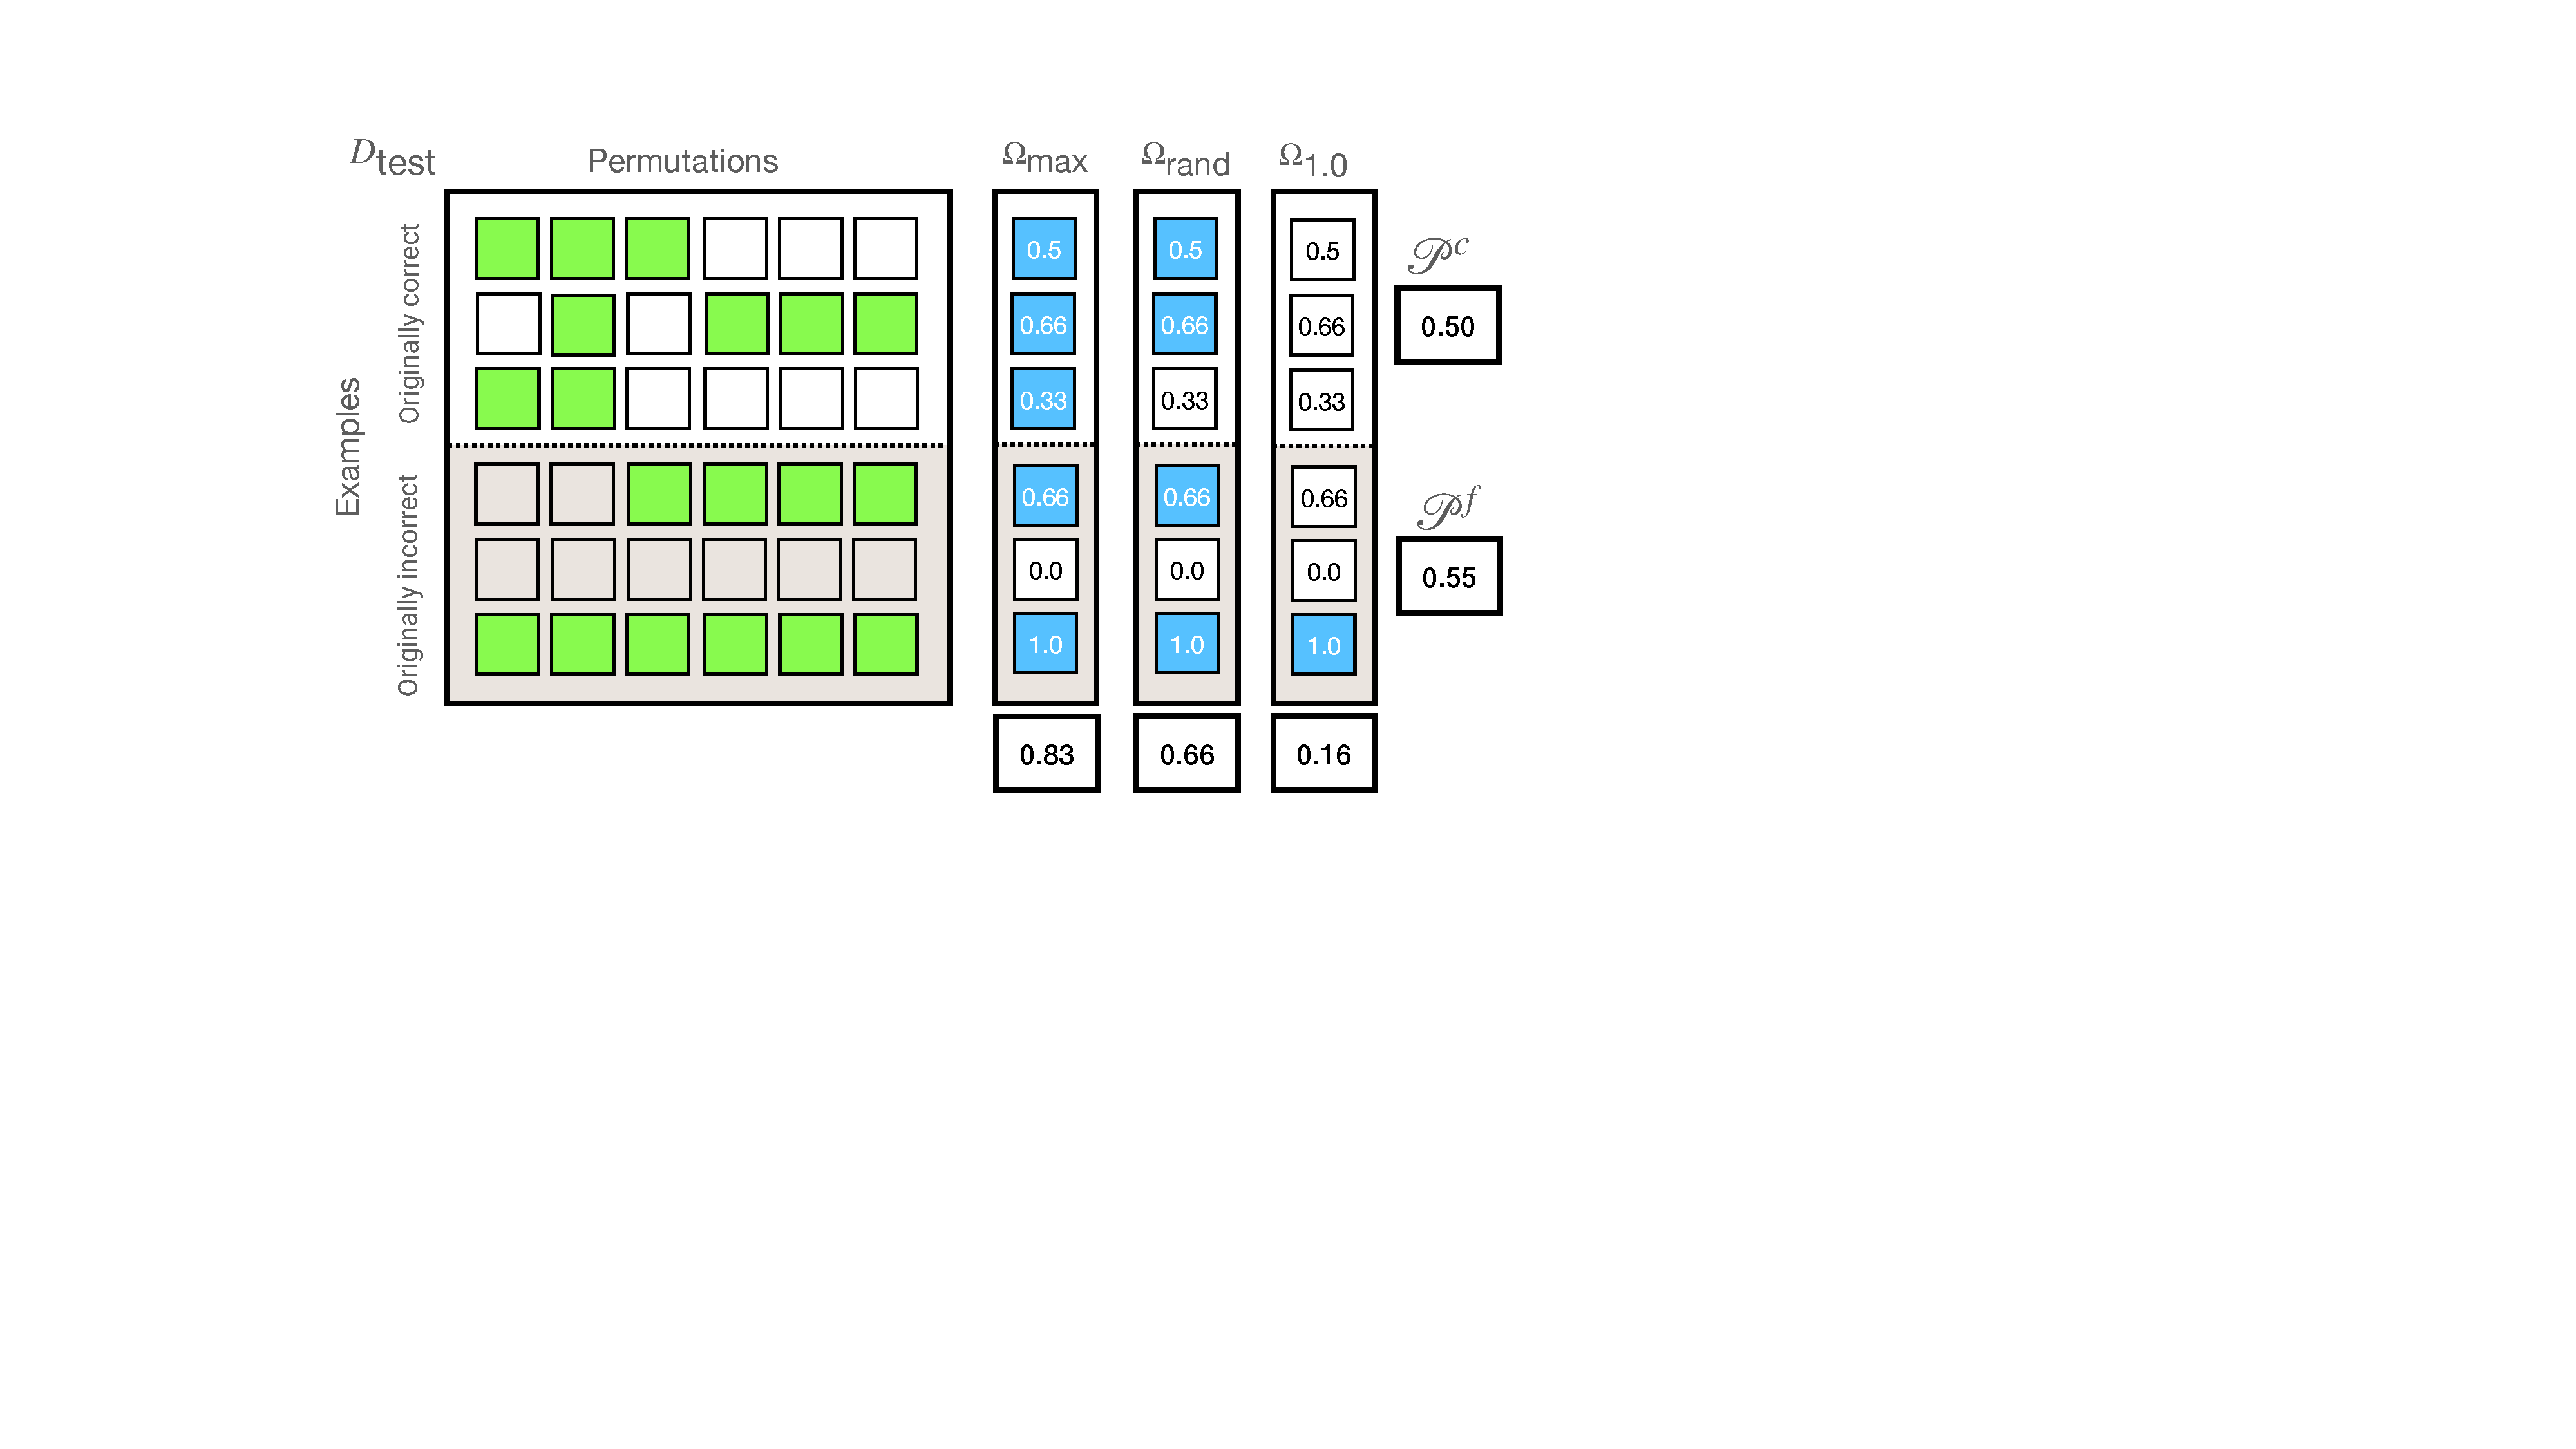
\includegraphics{figs/unli/nli_gen_perm_desc.pdf}}
    \caption{Graphical representation of the \PermAcc\ class of metrics. Given a sample test set ${D}_{\text{test}}$ with six examples, three of which originally predicted correctly (model predicts gold label), three incorrectly (model fails to predict gold label), with $n=6$ permutations, $\Omega_{\text{max}}$,$\Omega_{\text{rand}}$, $\Omega_{\text{1.0}}$, $\mathcal{P}^c$ and $\mathcal{P}^f$ are provided. Green boxes indicate permutations accepted by the model. Blue boxes mark examples that crossed each threshold and were used to compute the corresponding metric. }
    \label{fig:def_metrics}
\end{figure}

Let $\Pr_{M}(\hat{P}_i, \hat{H}_i)_{\text{cor}}$ then be the percentage of $q$ permutations of an example $(p_i, h_i)$ assigned the ground truth label $y_i$ by $M$:
   % \begin{equation}
    %\begin{split}
    \begin{align}
    &&\Pr_{M}(\hat{P}_i, \hat{H}_i)_{\text{cor}} =
    \frac{1}{q}\sum_{\mathclap{(\hat{p}_j \in \hat{P}_i, \hat{h}_j \in \hat{H}_i)}}((M(\hat{p}_j, \hat{h}_j) = y_i) \rightarrow 1)
    \end{align}
    %\end{split}
    %\end{equation}
To get an overall summary score, we let $\Omega_x$ be the percentage of examples $(p_i, h_i) \in D_{\text{test}}$ for which $\Pr_{M}(\hat{P}_i, \hat{H}_i)_{\text{cor}}$ exceeds a predetermined threshold $0 < x < 1$. %Concretely, $\Omega_x$ is defined as the percentage of examples in $D_{\text{test}}$, for which the probability of model accepting the permutation as the correct answer is greater than $x$ percent.
Concretely, a given example will count as correct according to $\Omega_x$ if more than $x$ percent of its permutations ($\hat{P}_i$ and $\hat{H}_i$) are assigned $y_i$ by the model $M$.
Mathematically,
    \begin{align} %I don't love this, but it fits...\mathrlap right centers the subscript, if it's centered it overlaps the D_test
    %\begin{split}
    &&\Omega_x = \frac{1}{\mid D_{test}\mid} \sum_{\mathrlap{(p_i, h_i)\in D_{test}}} ((\Pr_{M}(\hat{P}_i, \hat{H}_i)_{\text{cor}}
    > x) \rightarrow 1).
    %\end{split}
    \end{align}
There are two specific cases of $\Omega_{\text{x}}$ that we are most interested in. First, we define $\Omega_{\text{max}}$ or the \textbf{Maximum Accuracy}, where $x = 1 / |D_{\text{test}}|$. In short, $\Omega_{\text{max}}$ gives the percentage of examples $(p_i, h_i) \in D_{\text{test}}$ for which there is \textit{at least one} permutation $(\hat{p_j}, \hat{h_j})$ that model $M$ assigns the gold label $y_i$
% new: added comment on omega_max tending towards 1
\footnote{Theoretically, $\Omega_{\text{max}} \rightarrow 1$ if the number of permutations $q$ is large. Thus, in our experiments we set $q=100$.}.
Second, we define $\Omega_{\text{rand}}$, or \textbf{Random Baseline Accuracy}, where $x = 1 / m$ or chance probability (for balanced $m$-way classification, where $m=3$ in NLI). This metric is less stringent than $\Omega_{\text{max}}$, as it counts an example if at least \textit{one third} of its permutations are assigned the gold label (hence provides a lower-bound relaxation). See \autoref{fig:def_metrics} for a graphical representation of $\Omega_{\text{x}}$.

We also define %\textit{Flip}
$D^{f}$ to be the list of examples originally marked incorrect according to $\mathcal{A}$, but are now deemed correct according $\Omega_{\text{max}}$. $D^{c}$ is the list of examples originally marked correct according to  $\mathcal{A}$. Thus, we should expect $D^{f}<D^{c}$ for models that have high accuracy.
Additionally, we define $\mathcal{P}^c$ and $\mathcal{P}^f$, as the dataset average percentage of permutations which predicted the gold label, when the examples were originally correct ($D^{c}$) and when the examples were originally incorrect ($D^{f}$) as per $\mathcal{A}$ (hence, flipped) respectively.
\begin{equation}
\begin{split}
    &\mathcal{P}^{c} = \frac{1}{|D^{c}|} \sum_{i=0}^{|D^{c}|} M(\hat{P}_i, \hat{H}_i)_{\text{cor}}\\
    % &\mathcal{P}^f = \frac{1}{|D^{f}|} \sum_{i=0}^{|D^f|} M(\hat{P}_i, \hat{H}_i)_{\text{cor}}
\end{split}
\end{equation}

\noindent $P^f$ is defined similarly by replacing $D^c$ by $D^f$. Note that for a classic BOW model,  $\mathcal{P}^c=100$ and $\mathcal{P}^f=0$, because it would rely on the words alone (not their order) to make its classification decision. Since permuting removes no words, BOW models should come to the same decisions for permuted examples as for the originals.



\section{Evaluated Models}


We run our experiments on two types of models: \textbf{(a)} Transformer-based models and \textbf{(b)} Non-Transformer Models. In \textbf{(a)}, we investigate the state-of-the-art pre-trained models such as RoBERTa-Large \cite{liu-et-al-2019-roberta}, BART-Large \cite{lewis-etal-2020-bart} and DistilBERT \cite{sanh2020distilbert}. For \textbf{(b)} we consider several recurrent and convolution based neural networks, such as InferSent \cite{conneau-etal-2017-supervised}, Bidirectional LSTM \cite{collobert2008unified} and ConvNet \cite{zhao2015self}. We train all models on MNLI, and evaluate on in-distribution (SNLI and MNLI) and out-of-distribution datasets (ANLI). We independently verify results of \textbf{(a)} using both our fine-tuned model using HuggingFace Transformers \cite{wolf2020transformers} and pre-trained checkpoints from FairSeq \cite{ott2019fairseq} (using PyTorch Model Hub). For \textbf{(b)}, we use the InferSent codebase. We sample $q=100$ permutations for each example in $D_{\text{test}}$, and use 100 seeds for each of those permutations to ensure full reproducibility. We drop examples from test sets where we are unable to compute \textit{all unique} randomizations, typically these are examples with sentences of length of less than 6 tokens. \footnote{Code, data, and model checkpoints are available at \href{https://github.com/facebookresearch/unlu}{https://github.com/facebookresearch/unlu}.}



\section{Results}
\label{sec:unli_results}

\subsection{Models accept many permuted examples.}
\label{sec:unli_results_accept}

\begin{figure}[ht]
    \centering
    \resizebox{0.7\linewidth}{!}{
        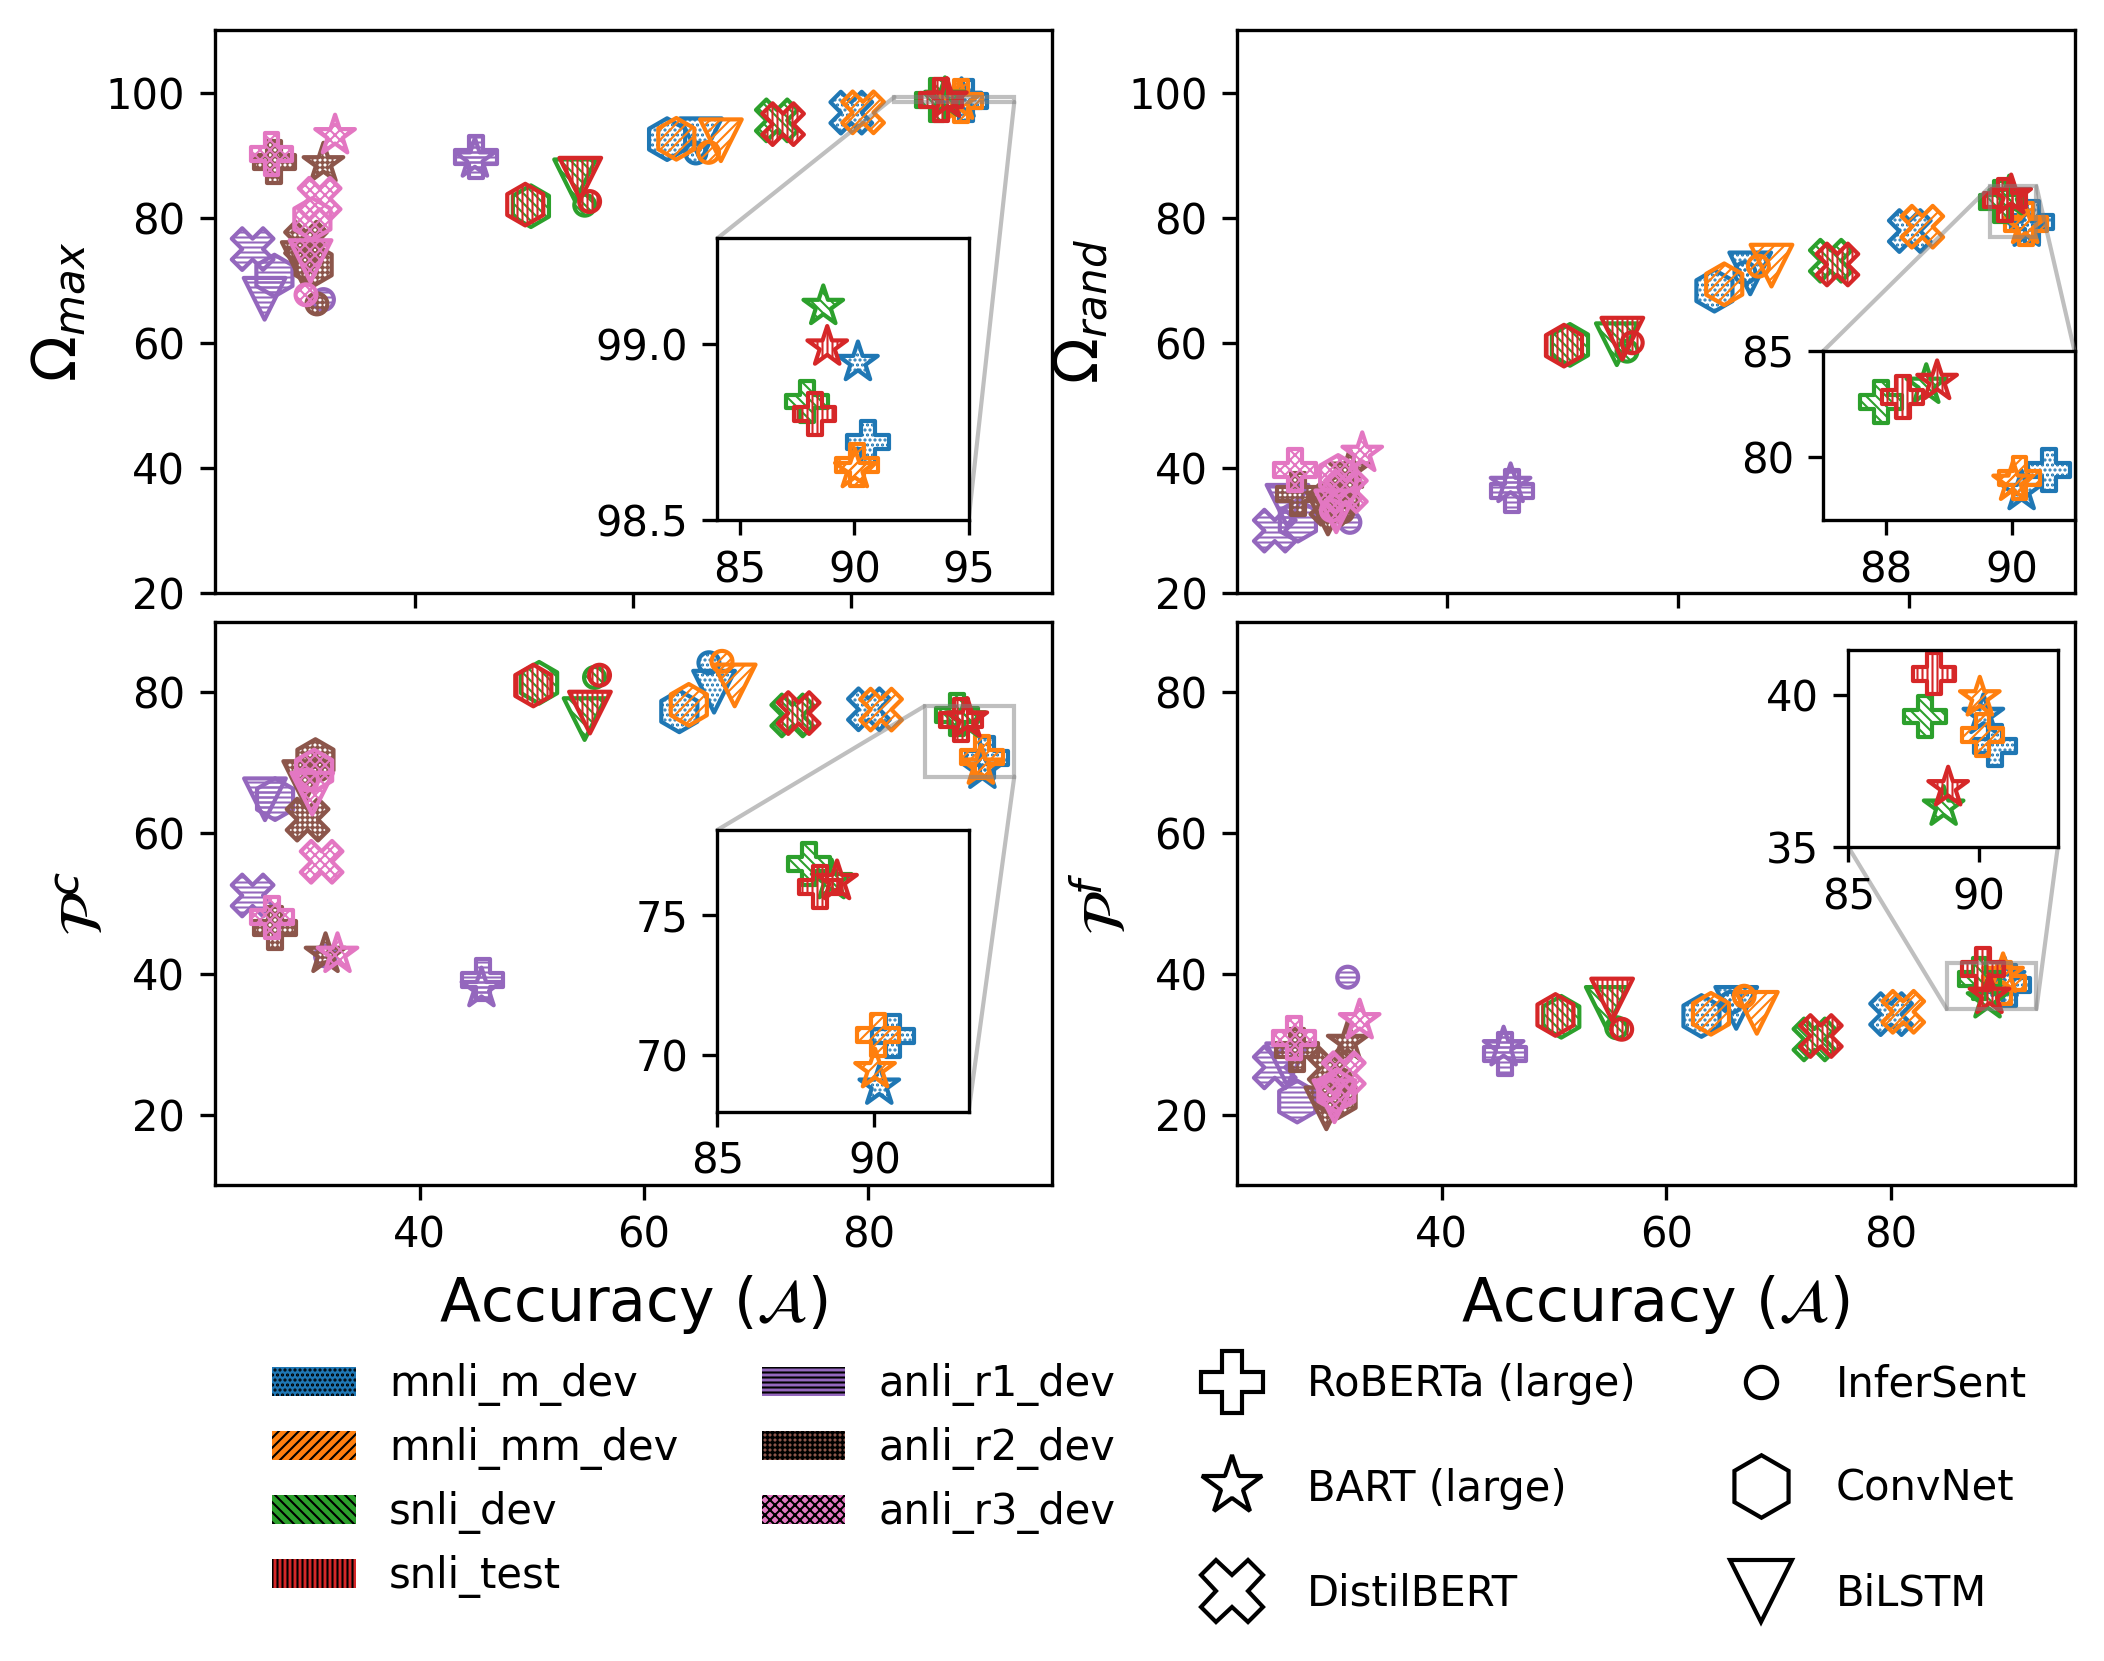
\includegraphics{figs/unli/comb_plot_0.png}}
    \caption{Comparison of $\Omega_{\text{max}}$,$\Omega_{\text{rand}}$,$\mathcal{P}^c$ and $\mathcal{P}^f$ with the model accuracy $\mathcal{A}$ on multiple datasets, where all models are trained on the MNLI corpus \cite{williams-etal-2018-broad}.}
    \label{fig:comb_plot}
\end{figure}

We find $\Omega_{\text{max}}$ is very high for models trained and evaluated on MNLI (in-domain generalization), reaching \textbf{98.7\%} on MNLI dev. and test sets (in RoBERTa, compared to $\mathcal{A}$ of 90.6\% (\autoref{table:unli_main}). Recall, human accuracy is approximately 92\% on MNLI dev.,  \citealt{nangia-bowman-2019-human}). This shows that there exists at least one permutation (usually many more) for almost all examples in $D_{\text{test}}$ such that model $M$ predicts the gold label. We also observe high $\Omega_{\text{rand}}$ at 79.4\%, showing that there are many examples for which the models outperform even a random baseline in accepting permuted sentences. We provide an example of the behaviour in \autoref{tab:unli:example}.

Evaluating out-of-domain generalization with ANLI dataset splits resulted in an $\Omega_{\text{max}}$ value that is notably higher than $\mathcal{A}$ (89.7\% $\Omega_{\text{max}}$ for RoBERTa compared to 45.6\% $\mathcal{A}$). As a consequence, we encounter many \textit{flips}, i.e., examples where the model is unable to predict the gold label, but at least one permutation of that example is able to. However, recall this analysis expects us to know the gold label upfront, so this test can be thought of as running a word-order probe test on the model until the model predicts the gold label (or give up by exhausting our set of $q$ permutations). For out-of-domain generalization, $\Omega_{\text{rand}}$ decreases considerably (36.4\% $\Omega_{\text{rand}}$ on A1), which means fewer permutations are accepted by the model. Next, recall that a classic bag-of-words model would have $\mathcal{P}^c=100$ and $\mathcal{P}^f=0$. No model performs strictly like a classic bag of words although they do perform somewhat BOW-like ($\mathcal{P}^c >> \mathcal{P}^f$ for all test splits, \autoref{fig:comb_plot}). %Although it is harder to find the correct permutation for already misclassified, non-generalizable sentences, state-of-the-art models still behave somewhat BOW-like.
We find this BOW-likeness to be higher for certain non-Transformer models, (InferSent) as they exhibit higher $\mathcal{P}^c$ (84.2\% for InferSent compared to 70.7\% for RoBERTa on MNLI).


\begin{table}[htbp]
  \centering
  \resizebox{0.5\linewidth}{!}{%
    \begin{tabular}{@{}llrrrrr@{}}
\toprule
           Model &    Eval. Dataset  &  $\mathcal{A}$ &  $\Omega_{\text{max}}$ &  $\mathcal{P}^c$ &  $\mathcal{P}^f$ &  $\Omega_{\text{rand}}$ \\
\midrule
\multirow{7}{*}{\bf RoBERTa-Large} 
 &   MNLI\_m\_dev &              0.906 &         0.987 &                  0.707 &             0.383 &                        0.794 \\
 &  MNLI\_mm\_dev &              0.901 &         0.987 &                  0.707 &             0.387 &                        0.790 \\
 &     SNLI\_dev &              0.879 &         0.988 &                  0.768 &             0.393 &                        0.826 \\
 &    SNLI\_test &              0.883 &         0.988 &                  0.760 &             0.407 &                        0.828 \\
 &  A1* &              0.456 &         0.897 &                  0.392 &             0.286 &                        0.364 \\
 &  A2* &              0.271 &         0.889 &                  0.465 &             0.292 &                        0.359 \\
 &  A3* &              0.268 &         0.902 &                  0.480 &             0.308 &                        0.397 \\ \midrule
 & Mean & 0.652 & 0.948 & 0.611 & \boldred{0.351} & 0.623 \\ 
% & Harmonic Mean & 0.497 & 0.946 & 0.572 & 0.344 & 0.539 \\ 
\midrule
 
\multirow{7}{*}{\bf BART-Large} 
    &   MNLI\_m\_dev &              0.902 &         0.989 &                  0.689 &             0.393 &                        0.784 \\
    &  MNLI\_mm\_dev &              0.900 &         0.986 &                  0.695 &             0.399 &                        0.788 \\
    &     SNLI\_dev &              0.886 &         0.991 &                  0.762 &             0.363 &                        0.834 \\
    &    SNLI\_test &              0.888 &         0.990 &                  0.762 &             0.370 &                        0.836 \\
    &  A1* &              0.455 &         0.894 &                  0.379 &             0.295 &                        0.374 \\
    &  A2* &              0.316 &         0.887 &                  0.428 &             0.303 &                        0.397 \\
    &  A3* &              0.327 &         0.931 &                  0.428 &             0.333 &                        0.424 \\ \midrule
& Mean &  \textbf{0.668} & \boldred{0.953} & 0.592 & \boldred{0.351} & \boldred{0.634} \\
%& Harmonic Mean &  \textbf{0.543} & \boldred{0.951} & 0.546 & \boldred{0.347} & \boldred{0.561} \\ 
\midrule
\multirow{7}{*}{\bf DistilBERT}  &   MNLI\_m\_dev &              0.800 &         0.968 &                  0.775 &             0.343 &                        0.779 \\
      &  MNLI\_mm\_dev &              0.811 &         0.968 &                  0.775 &             0.346 &                        0.786 \\
      &     SNLI\_dev &              0.732 &         0.956 &                  0.767 &             0.307 &                        0.731 \\
      &    SNLI\_test &              0.738 &         0.950 &                  0.770 &             0.312 &                        0.725 \\
      &  A1* &              0.251 &         0.750 &                  0.511 &             0.267 &                        0.300 \\
      &  A2* &              0.300 &         0.760 &                  0.619 &             0.265 &                        0.343 \\
      &  A3* &              0.312 &         0.830 &                  0.559 &             0.259 &                        0.363 \\ \midrule
      & Mean &  0.564 & 0.883 & \boldred{0.682} & 0.300 & 0.575 \\ 
%& Harmonic Mean &  0.445 & 0.873 & \boldred{0.664} & 0.296 & 0.490 \\
% \bottomrule
\midrule\midrule
 \multirow{7}{*}{\bf InferSent} 
 &   MNLI\_m\_dev &              0.658 &         0.904 &                  0.842 &             0.359 &                        0.712 \\
 &  MNLI\_mm\_dev &              0.669 &         0.905 &                  0.844 &             0.368 &                        0.723 \\
 &     SNLI\_dev &              0.556 &         0.820 &                  0.821 &             0.323 &                        0.587 \\
 &    SNLI\_test &              0.560 &         0.826 &                  0.824 &             0.321 &                        0.600 \\
 &  A1* &              0.316 &         0.669 &                  0.425 &             0.395 &                        0.313 \\
 &  A2* &              0.310 &         0.662 &                  0.689 &             0.249 &                        0.330 \\
 &  A3* &              0.300 &         0.677 &                  0.675 &             0.236 &                        0.332 \\ \midrule
 & Mean &  \textbf{0.481} & 0.780 & 0.731 & \boldred{0.322} & 0.514 \\ 
 %& Harmonic Mean &  0.429 & 0.767 & 0.694 & \boldred{0.311} & 0.455 \\ 
 \midrule
 \multirow{7}{*}{\bf ConvNet}
 &   MNLI\_m\_dev &              0.631 &         0.926 &                  0.773 &             0.340 &                        0.684 \\
 &  MNLI\_mm\_dev &              0.640 &         0.926 &                  0.782 &             0.343 &                        0.694 \\
 &     SNLI\_dev &              0.506 &         0.819 &                  0.813 &             0.339 &                        0.597 \\
 &    SNLI\_test &              0.501 &         0.821 &                  0.809 &             0.341 &                        0.596 \\
 &  A1* &              0.271 &         0.708 &                  0.648 &             0.218 &                        0.316 \\
 &  A2* &              0.307 &         0.725 &                  0.703 &             0.224 &                        0.356 \\
 &  A3* &              0.306 &         0.798 &                  0.688 &             0.234 &                        0.388 \\ \midrule
 & Mean &  0.452 & \boldred{0.817} & \boldred{0.745} & 0.291 & 0.519 \\ 
%& Harmonic Mean &  0.404 & \boldred{0.810} & \boldred{0.740} & 0.279 & \boldred{0.473} \\ 
\midrule
 \multirow{7}{*}{\bf BiLSTM} 
 &   MNLI\_m\_dev &              0.662 &         0.925 &                  0.800 &             0.351 &                        0.711 \\
 &  MNLI\_mm\_dev &              0.681 &         0.924 &                  0.809 &             0.344 &                        0.724 \\
 &     SNLI\_dev &              0.547 &         0.860 &                  0.762 &             0.351 &                        0.598 \\
 &    SNLI\_test &              0.552 &         0.862 &                  0.771 &             0.363 &                        0.607 \\
 &  A1* &              0.262 &         0.671 &                  0.648 &             0.271 &                        0.340 \\
 &  A2* &              0.297 &         0.728 &                  0.672 &             0.209 &                        0.328 \\
 &  A3* &              0.304 &         0.731 &                  0.656 &             0.219 &                        0.331 \\ \midrule
 & Mean &  0.472 & 0.814 & 0.731 & 0.301 & \boldred{0.520} \\
%& Harmonic Mean &  0.410 & 0.803 & 0.725 & 0.287 & 0.463 \\
 
\bottomrule
\end{tabular}}
  \caption{Statistics for Transformer-based models trained on MNLI corpus \cite{williams-etal-2018-broad}. 
  %$\Omega_{\text{max}}$ or Max Accuracy is computed if \textit{any} of the $n=100$ permutations per data point yield correct results. The mean number of permutations which were correct, when the original prediction is correct or incorrect  are given by $\mathcal{P}^c$  and $\mathcal{P}^f$ (flipped) respectively. $\Omega_{\text{rand}}$ is the percentage of data points for which models choose the ground truth label over a random uniform baseline (1/3). 
  The highest values are bolded (\boldred{red} indicates the model most insensitive to permutation) per metric and per model class (Transformers and non-Transformers). A1*, A2* and A3* refer to the ANLI dev. sets \citep{nie-etal-2020-adversarial}.}
  \label{table:unli_main}
\end{table}




\subsubsection{Investigating other $\Omega$ values}

\begin{figure*}
    \centering
    \resizebox{\textwidth}{!}{
        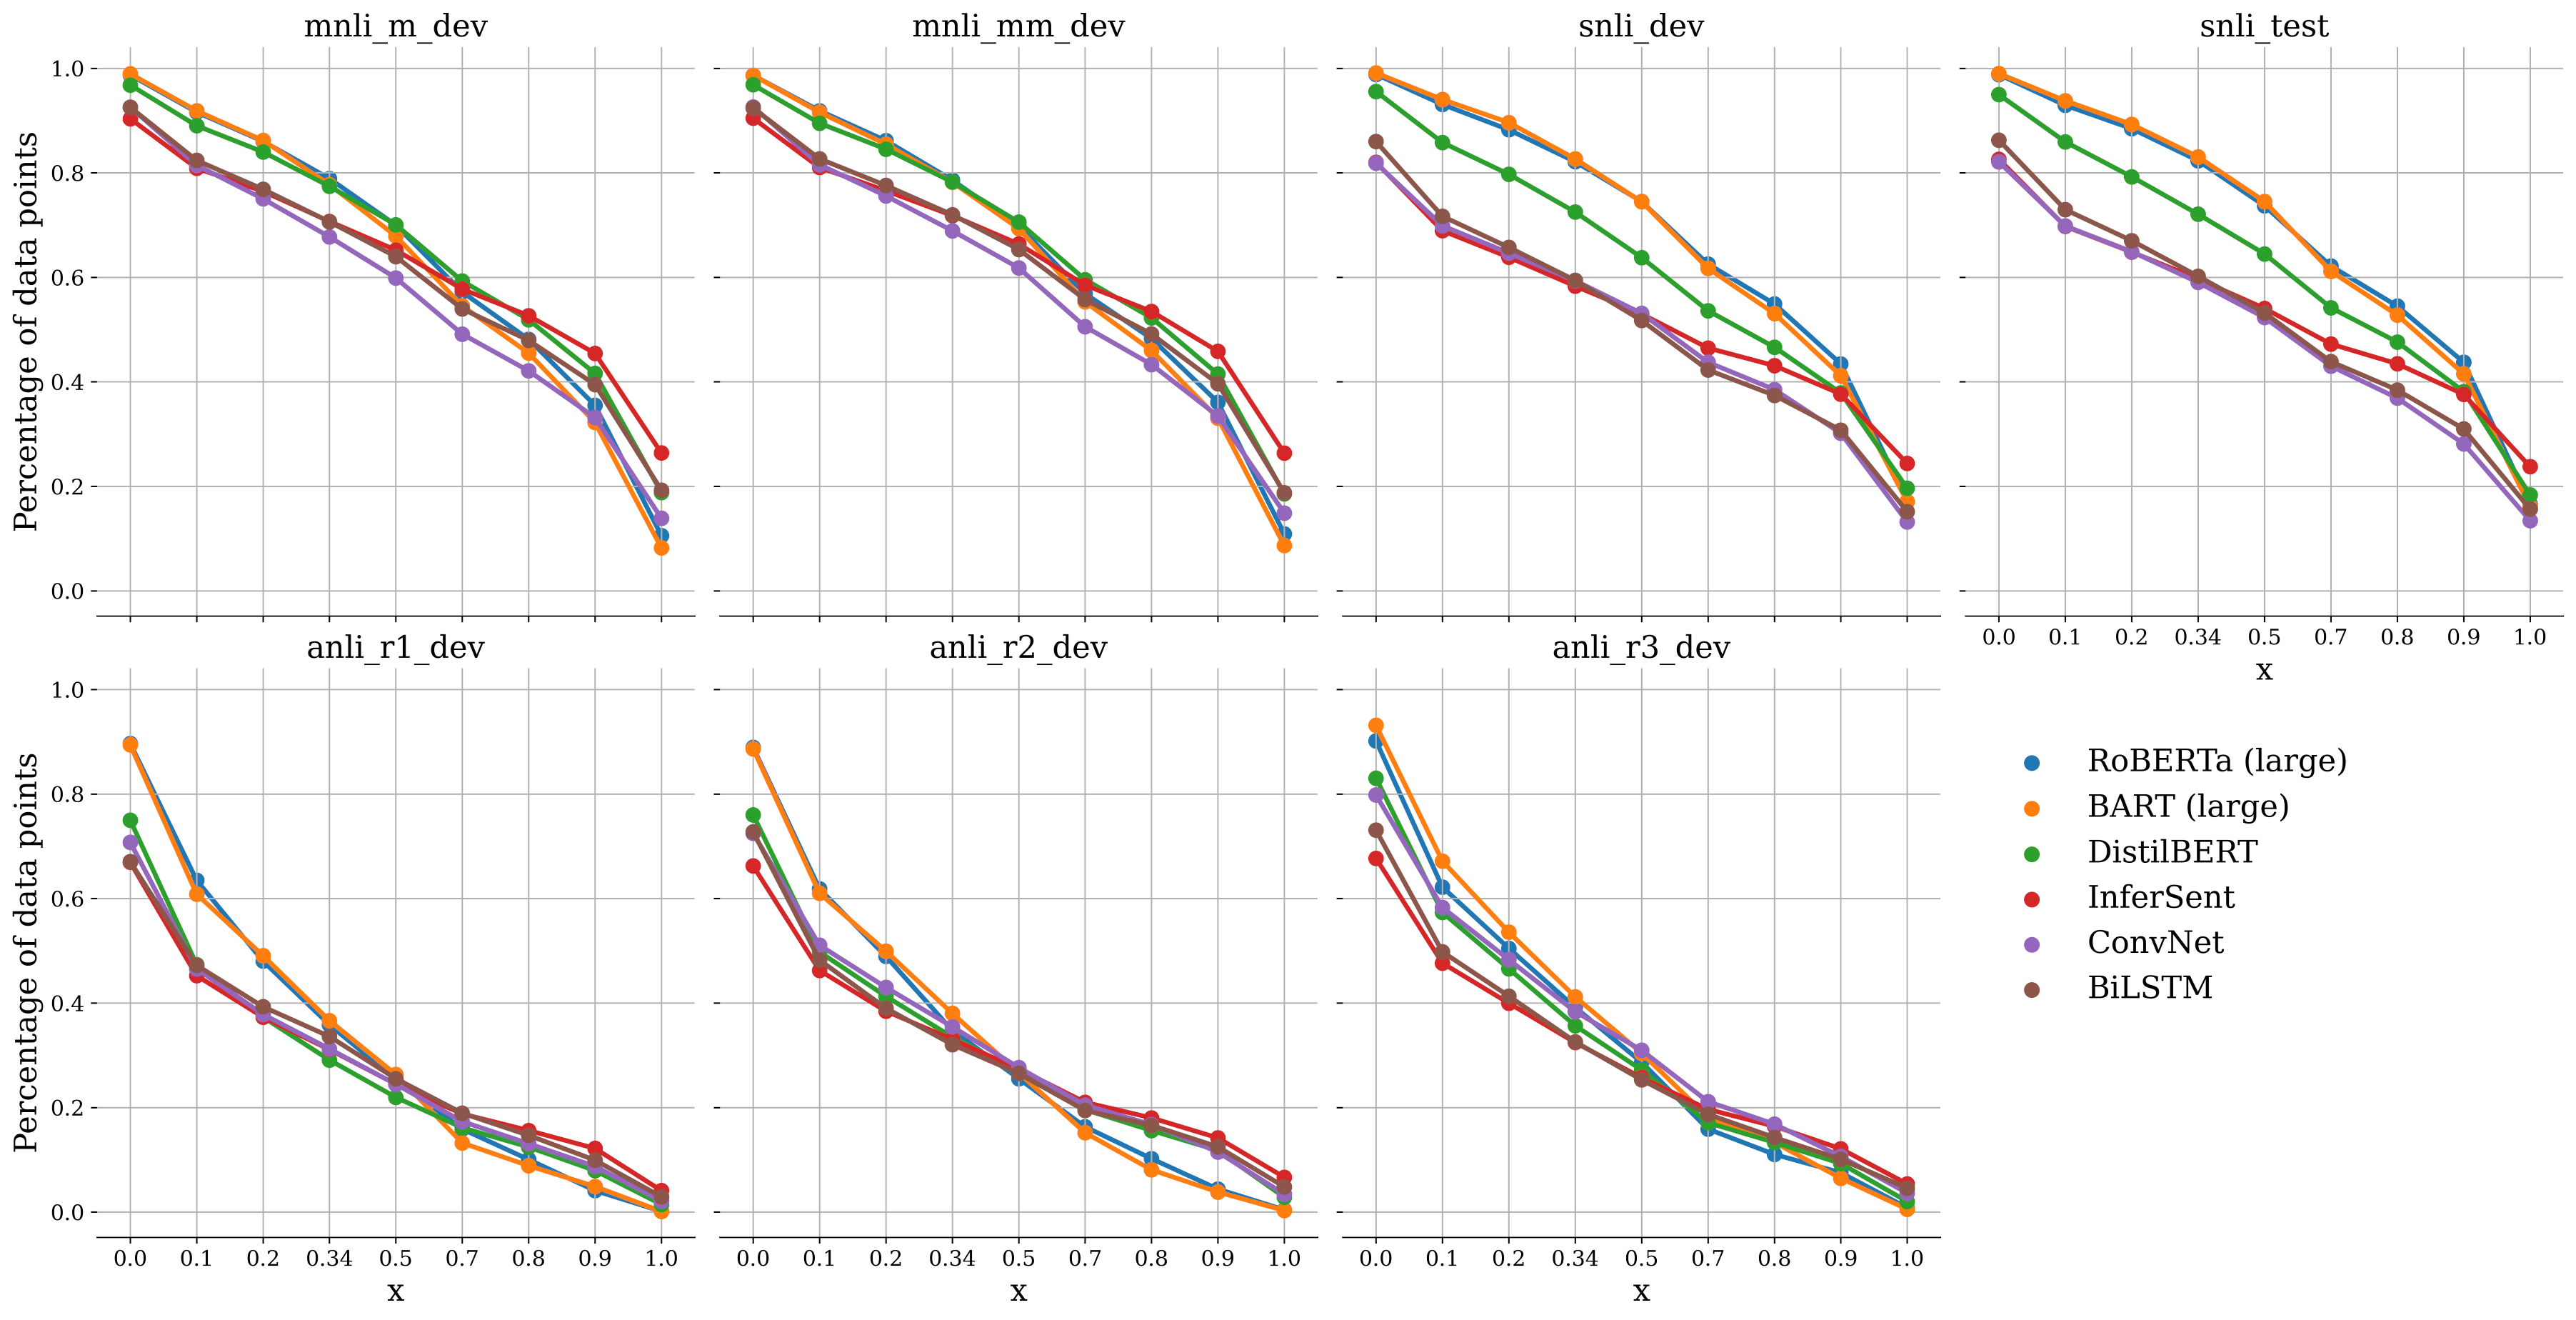
\includegraphics{figs/unli/omega_threshold.png}}
    \caption{$\Omega_x$ threshold for all datasets with varying $x$ and computing the percentage of examples that fall within the threshold. The top row consists of in-distribution datasets (MNLI, SNLI) and the bottom row contains out-of-distribution datasets (ANLI)}
    \label{fig:unli:threshold_omega_x}
\end{figure*}


We defined two variations of $\Omega_x$, $\Omega_{\text{max}}$ and $\Omega_{\text{rand}}$, but theoretically it is possible to define any arbitrary threshold percentage $x$ to evaluate the unnatural language inference mechanisms of different models. In \autoref{fig:unli:threshold_omega_x} we show the effect of different thresholds, including $\Omega_{\text{max}}$ where $x = 1/|D_{\text{test}|}$ and $\Omega_{\text{rand}}$ where $x = 0.34$. We observe for in-distribution datasets (top row, MNLI and SNLI splits), in the extreme setting when $x=1.0$, there are more than 10\% of examples available, and more than 25\% in case of InferSent and DistilBERT. For out-of-distribution datasets (bottom row, ANLI splits) we observe a much lower trend, suggesting generalization itself is the bottleneck in permuted sentence understanding.



\subsection{Models are very confident.}
\label{sec:unli_results_conf}

% Will it be too small?
\begin{figure}[t]
    \centering
    \resizebox{0.7\textwidth}{!}{
        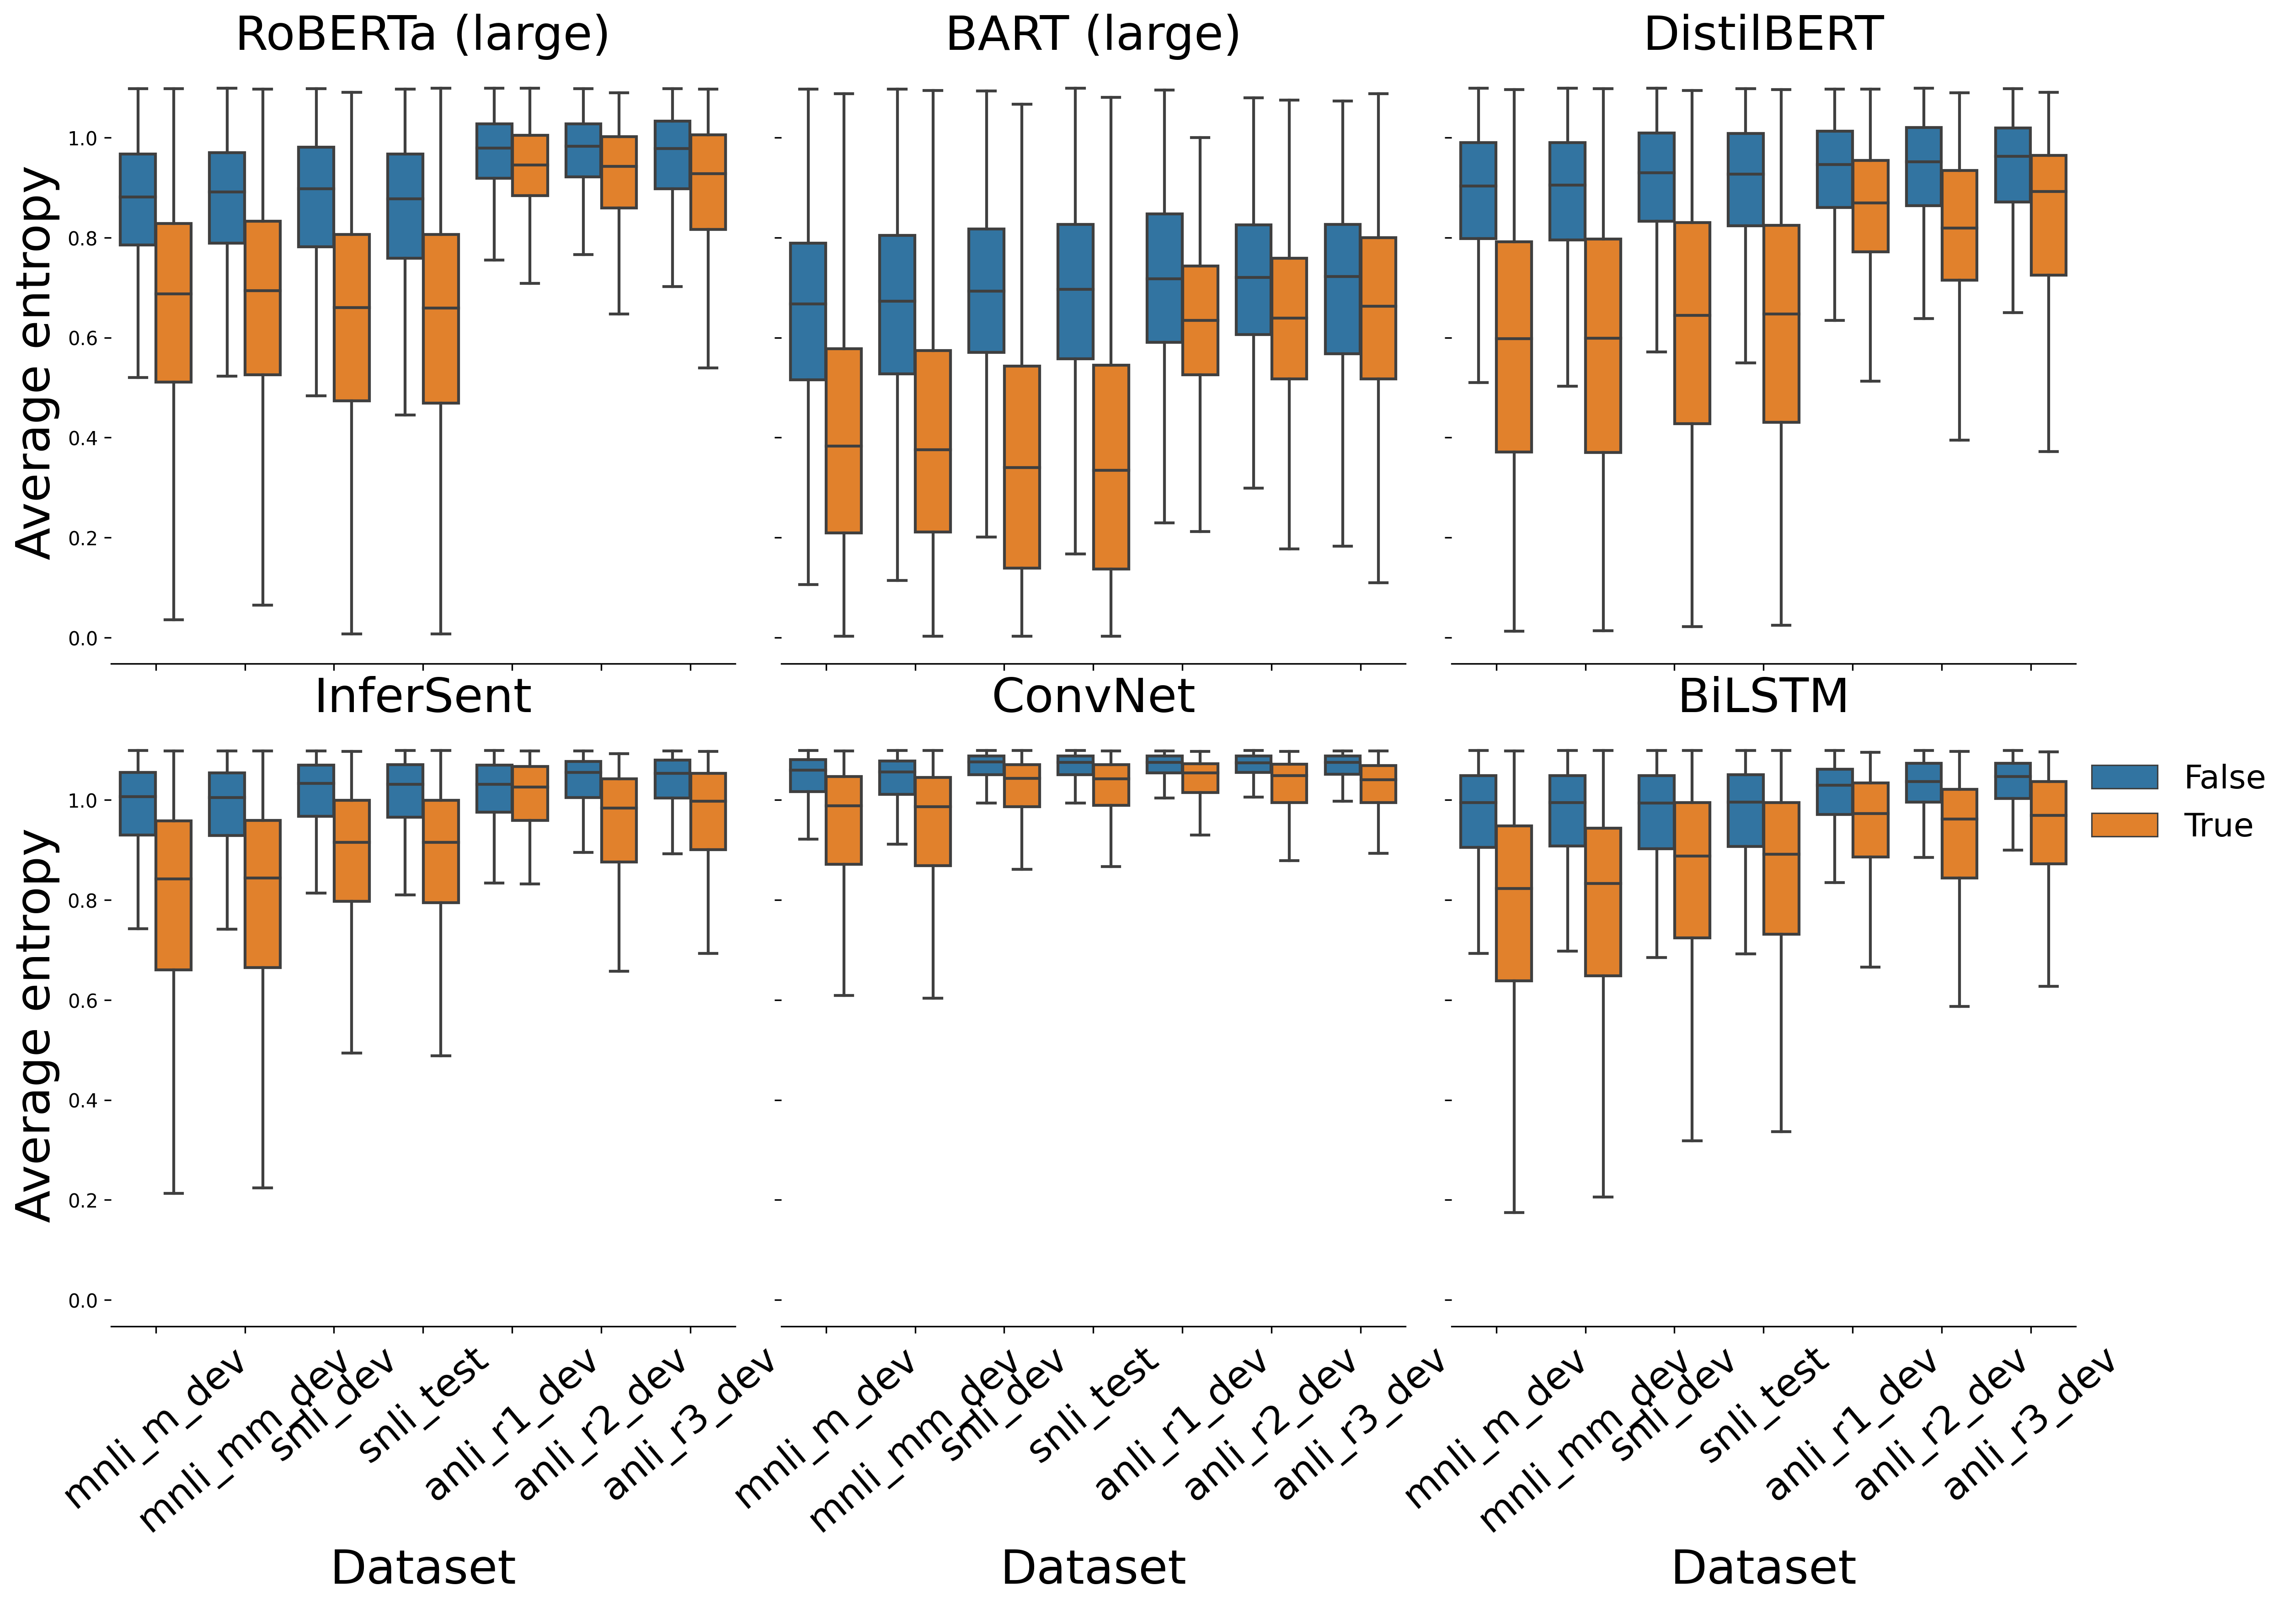
\includegraphics{figs/unli/entropy_plot.png}}
    \caption{Average entropy of model confidences on permutations that yielded the correct results for Transformer-based models (top) and Non-Transformer-based models (bottom). Results are shown for $D^c$ (orange) and $D^f$ (blue). The boxes show the quartiles of the entropy distributions.}
    \label{fig:unli_all_entropy}
\end{figure}


The phenomenon we observe would be of less concern if the correct label prediction was just an outcome of chance, which could occur when the entropy of the log probabilities of the model output is high (suggesting uniform probabilities on entailment, neutral and contradiction labels, recall Model B from \autoref{sec:unli_technical_bg}). We first investigate the model probabilities for the Transformer-based models on the permutations that lead to the correct answer in \autoref{fig:unli_all_entropy}. We find overwhelming evidence that model confidences on in-distribution datasets (MNLI, SNLI) are highly skewed, resulting in low entropy, and it varies among different model types. BART proves to be the most skewed Transformer-based model. This skewness is not a property of model capacity, as we observe DistilBERT log probabilities to have similar skewness as RoBERTa (large) model, while exhibiting lower $\mathcal{A}$, $\Omega_{\text{max}}$, and $\Omega_{\text{rand}}$.

% KS: I think this paper has the inverse result!
% The high confidence of Transformer-based model can be attributed to their tendency to be mis-calibrated in an out-of-domain setting, which is opposite to \newcite{desai2020calibration}!!!.

% [CHECK] comment on why Transformers are more confident. Find citations
% Do we know of a paper which shows Transformer entropies are low?
% Use the term calibration
% https://arxiv.org/pdf/2003.07892.pdf
% http://proceedings.mlr.press/v119/braverman20a/braverman20a.pdf

For non-Transformers whose accuracy $\mathcal{A}$ is lower, the $\Omega_{\text{max}}$ achieved by these models are also predictably lower. We observe roughly the same relative performance in the terms of $\Omega_{\text{max}}$ (\autoref{fig:comb_plot} and \autoref{table:unli_main}) and Average entropy (Figure \ref{fig:unli_all_entropy}). However, while comparing the averaged entropy of the model predictions, it is clear that there is some benefit to being a worse model---non-Transformer models are not as overconfident on randomized sentences as Transformers are.
High confidence of Transformer models can be attributed to the \textit{overthinking} phenomenon commonly observed in deep neural networks \cite{kaya2019shallowdeep} and BERT-based models \cite{zhou2020bert}.
% KS: I think this is a better reasoning? Please check.


\subsection{Similar artifacts in Chinese \acrshort{nlu}.}
\label{sec:unli_ocnli_results}

\begin{table}[htbp]
    \centering
    \footnotesize
    \resizebox{0.7\linewidth}{!}{%
        \begin{tabular}{llrrrrrr}
            \toprule
             Model              & $\mathcal{A}$ & $\Omega_{\text{max}}$ & $\mathcal{P}^c$ & $\mathcal{P}^f$ & $\Omega_{\text{rand}}$ \\ \midrule
             RoBERTa-Large   & \textbf{0.784} &         \boldred{0.988} &                  0.726 &             \boldred{0.339} &                        \boldred{0.773}            \\
             InferSent &             0.573 &         0.931 &                  0.771 &             0.265 &                        0.615 \\
   ConvNet &              0.407 &         0.752 &                  \boldred{0.808} &             0.199 &                        0.426 \\
    BiLSTM &              0.566 &         0.963 &                  0.701 &             0.271 &                        0.611 \\
            \bottomrule
        \end{tabular}}
    \caption{Results on evaluation on OCNLI Dev set. All models are trained on OCNLI corpus \cite{hu-etal-2020-ocnli}. 
    % Max accuracy ($\Omega_{\text{max}}$) is computed based on whether \textit{any} of the $n=100$ permutations per data point yield correct results. $\mathcal{P}^c$  stands for the mean number of permutations which were correct when the original prediction is correct. $\mathcal{P}^f$  stats for the mean number of permutations which are correct when the original prediction is incorrect (flip). 
    Bold marks the highest value per metric (\boldred{red} shows the model is insensitive to permutation).}
    \label{table:ocnli_all}
\end{table}


We extended the experiments to the Original Chinese NLI dataset \citep[OCNLI]{hu-etal-2020-ocnli}, and re-used the pre-trained RoBERTa-Large and InferSent (non-Transformer) models on OCNLI. Our findings are similar to the English results (\autoref{table:ocnli_all}), thereby suggesting that the phenomenon is not just an artifact of English text or tokenization.

\subsection{Other Results.} We investigated the effect of sentence length (which correlates with number of possible permutations), and hypothesis-only randomization (models exhibit similar phenomenon even when only hypothesis is permuted). In terms of sentence length, we observe that shorter sentences in general have a somewhat higher probability of acceptance for examples which was originally predicted correctly---since shorter sentences have fewer unique permutations (\autoref{fig:unli_length}). However, for the examples which were originally incorrect, the trend is not present.

\begin{figure}[ht]
    \centering
    \resizebox{0.8\textwidth}{!}{
      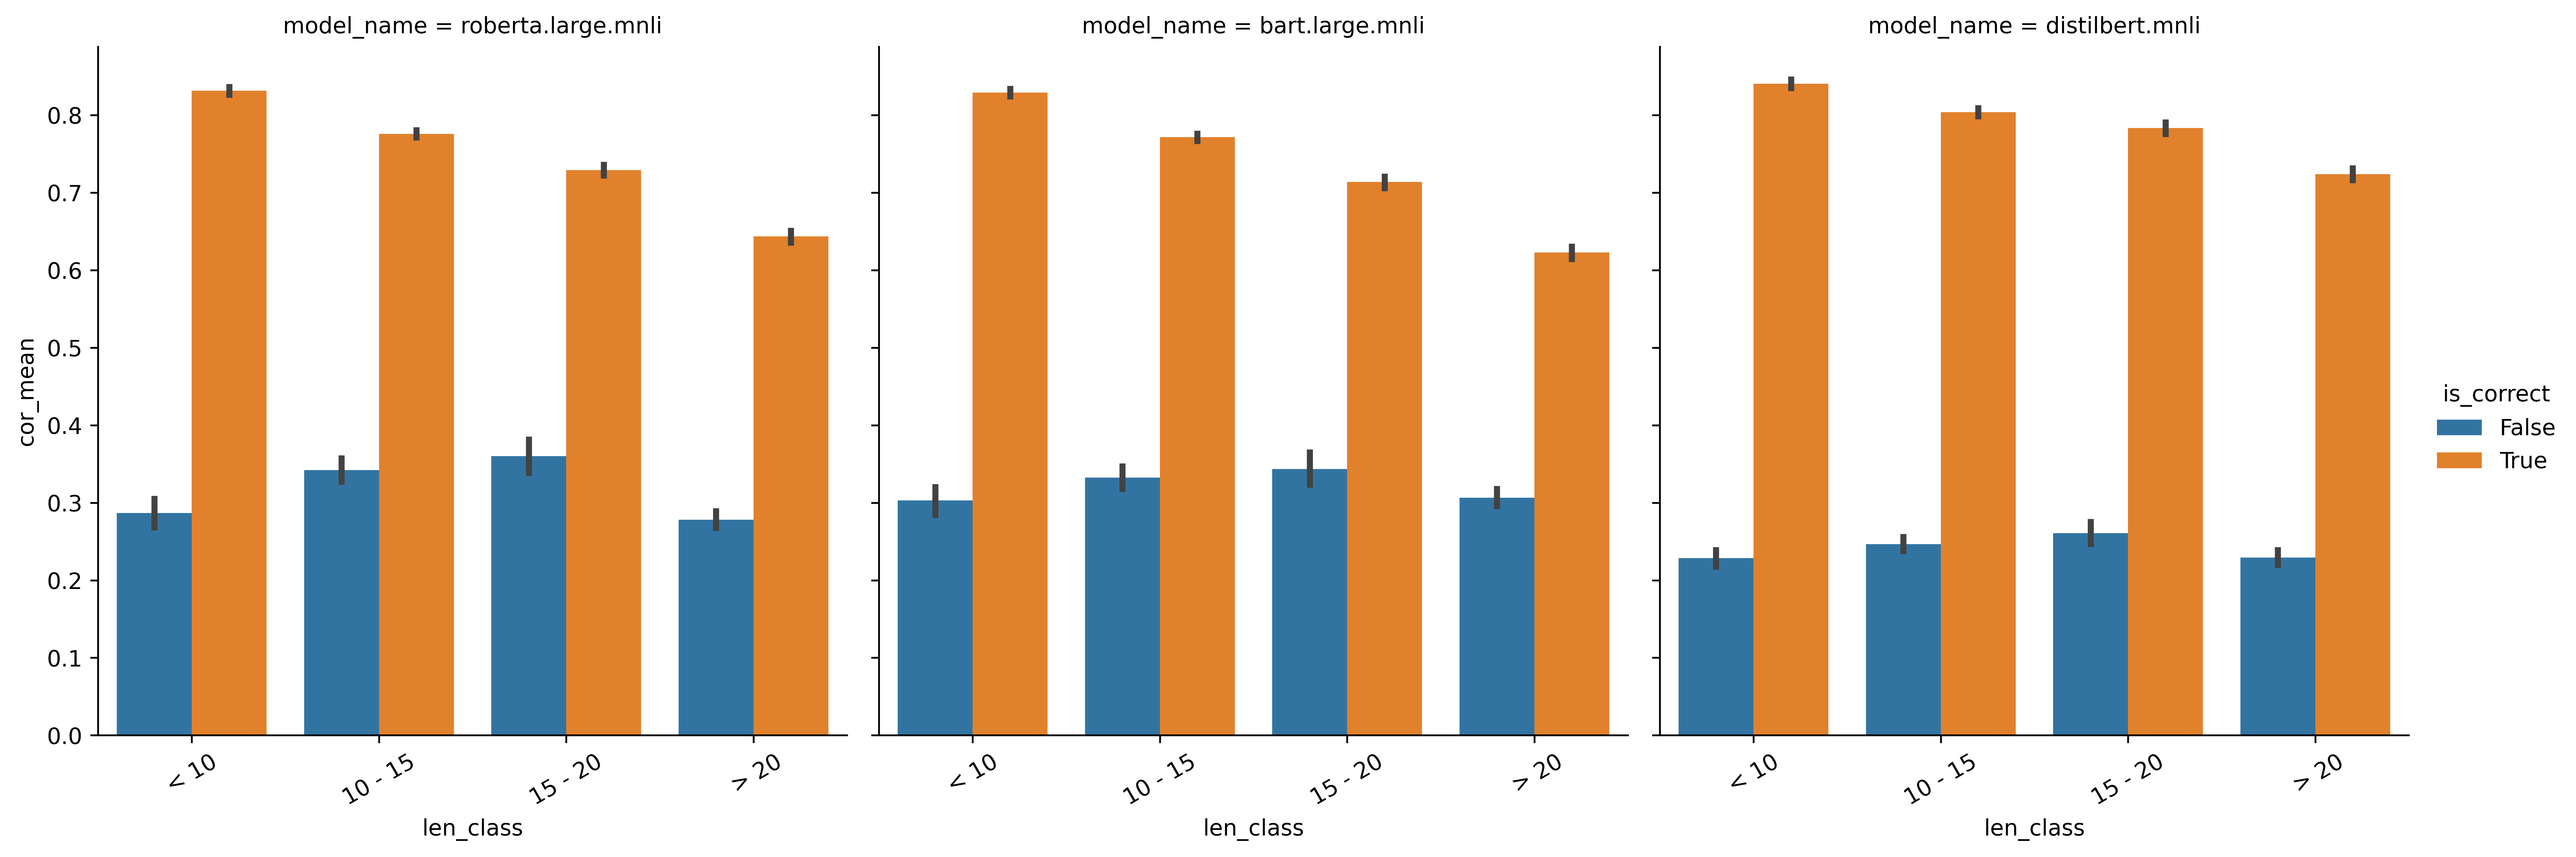
\includegraphics{figs/unli/transformer_length.png}
      % \includegraphics{example-image-a}
    }
    \caption{Length and \PermAcc by Transformer-based models.}
    \label{fig:unli_length}
\end{figure}

\begin{figure}[ht]
    \centering
    \resizebox{0.7\textwidth}{!}{
      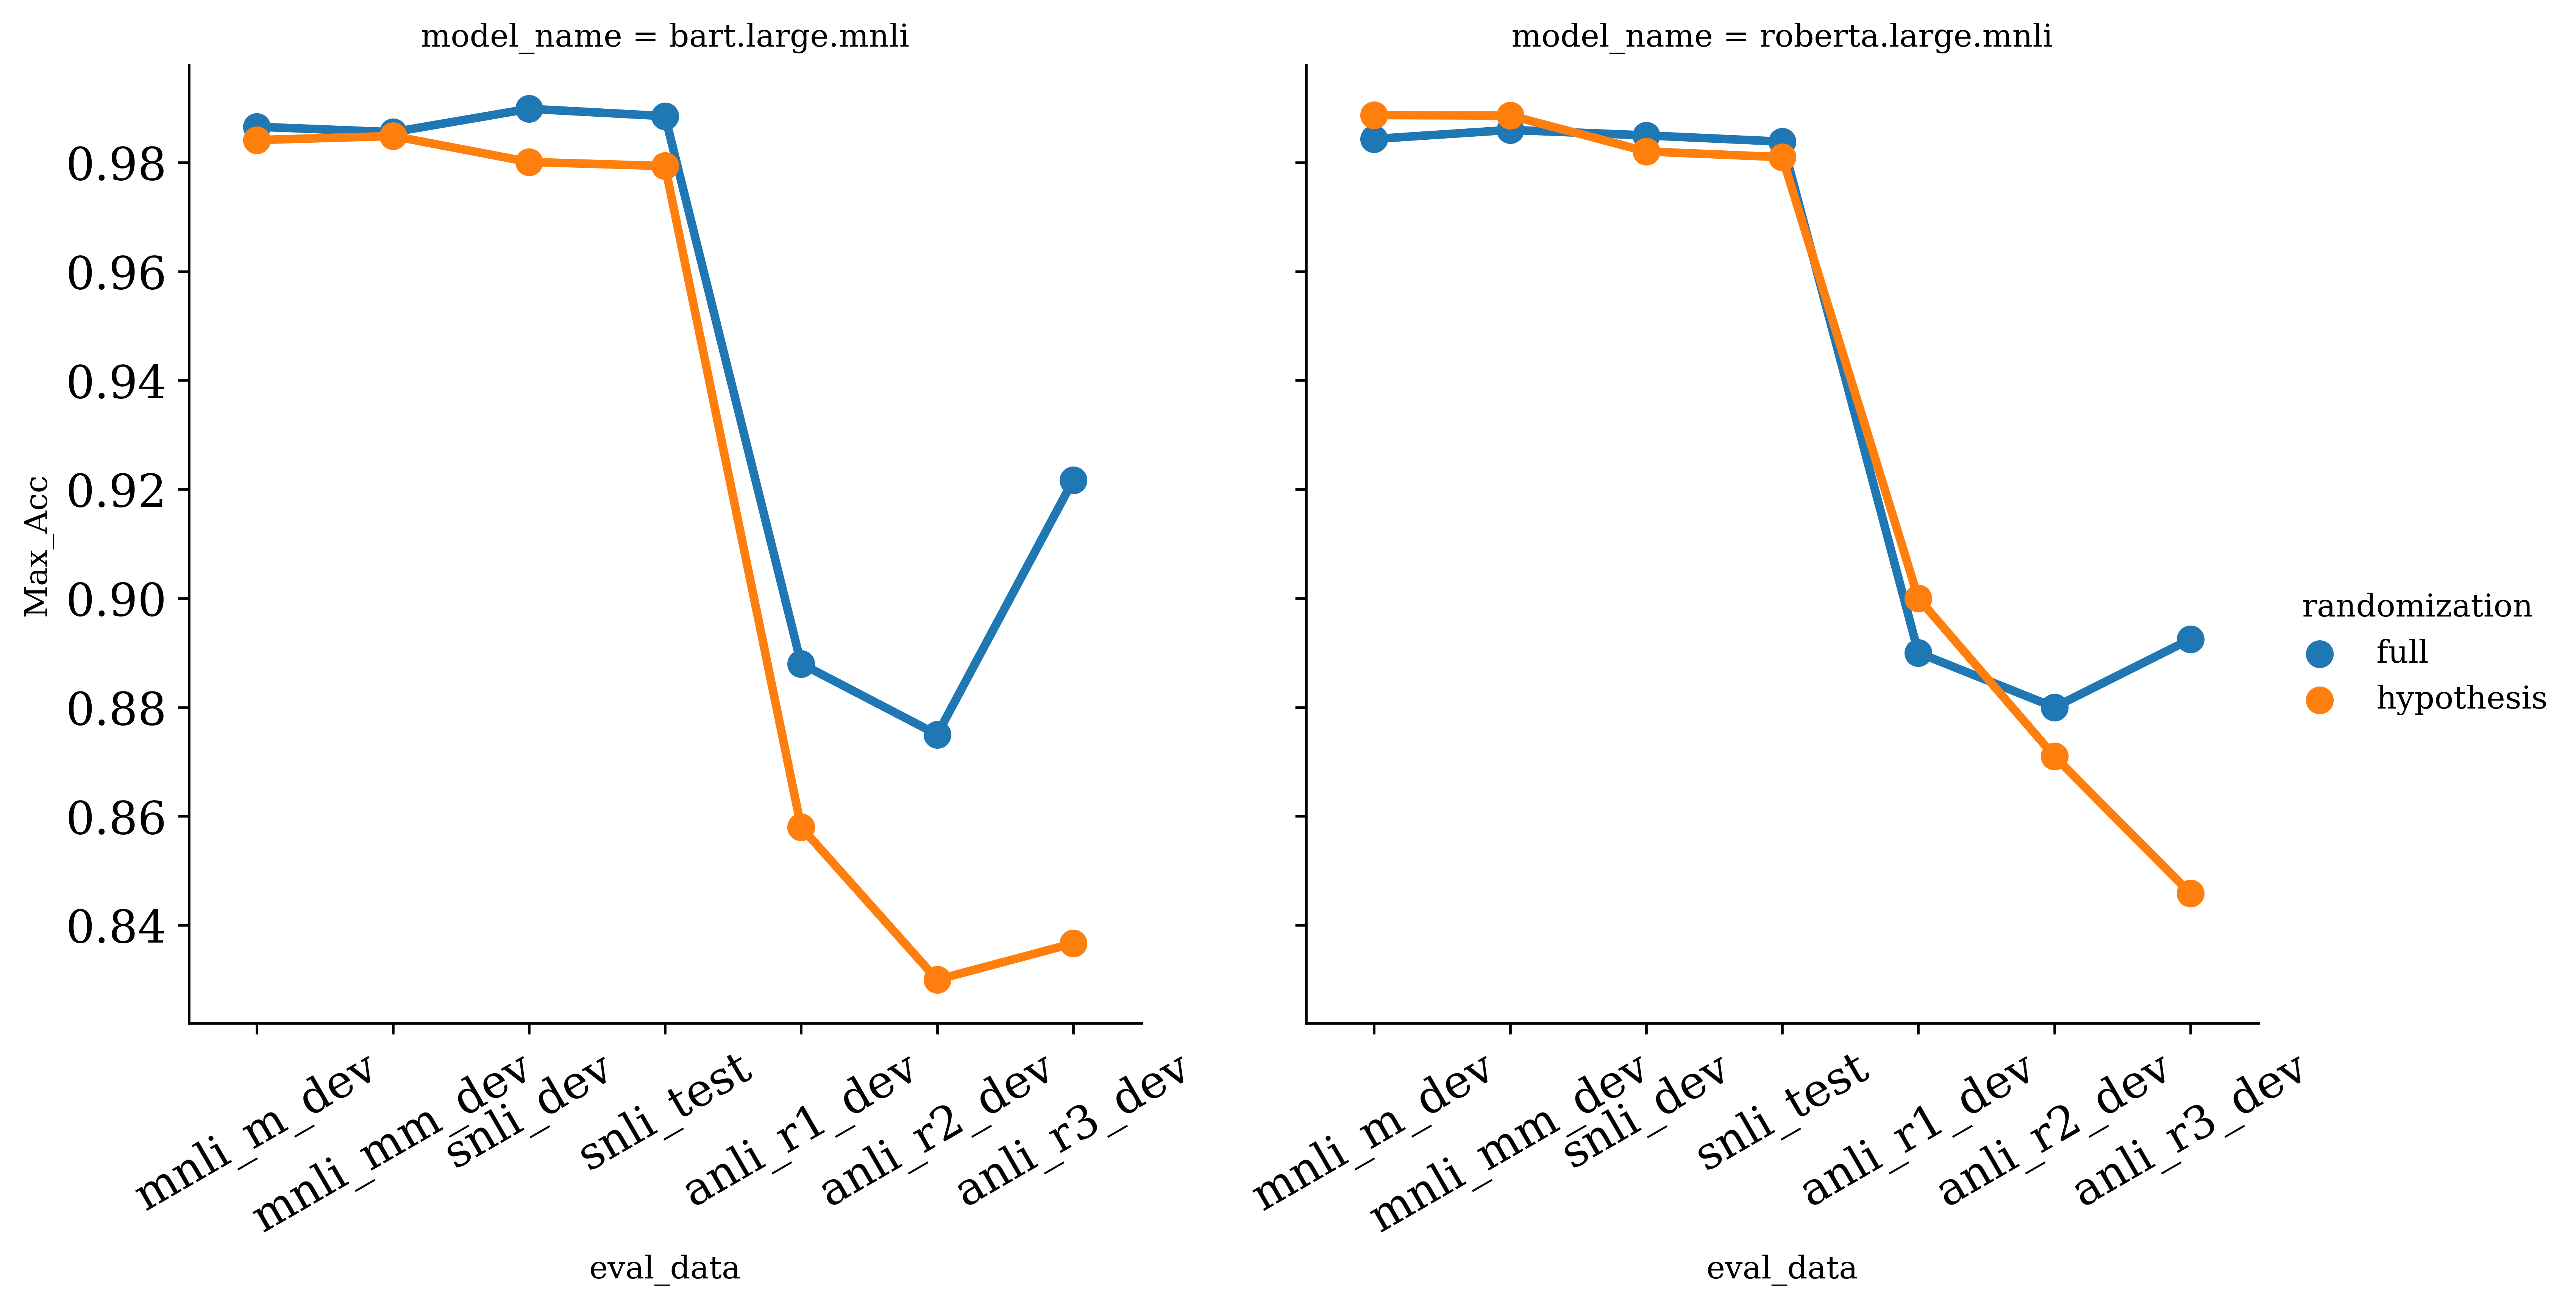
\includegraphics{figs/unli/hypothesis_compare.png}
    }
    \caption{Comparing the effect between randomizing both premise and hypothesis and only hypothesis on two Transformer-based models, RoBERTa and BART. Here, we observe the difference of $\Omega_{\text{max}}$ is marginal in in-distribution datasets (SNLI, MNLI), while hypothesis-only randomization is worse for out-of-distribution datasets (ANLI).}
    \label{fig:unli_hp_compare}
\end{figure}

\begin{figure}[ht]
  \centering
    \resizebox{0.7\textwidth}{!}{
      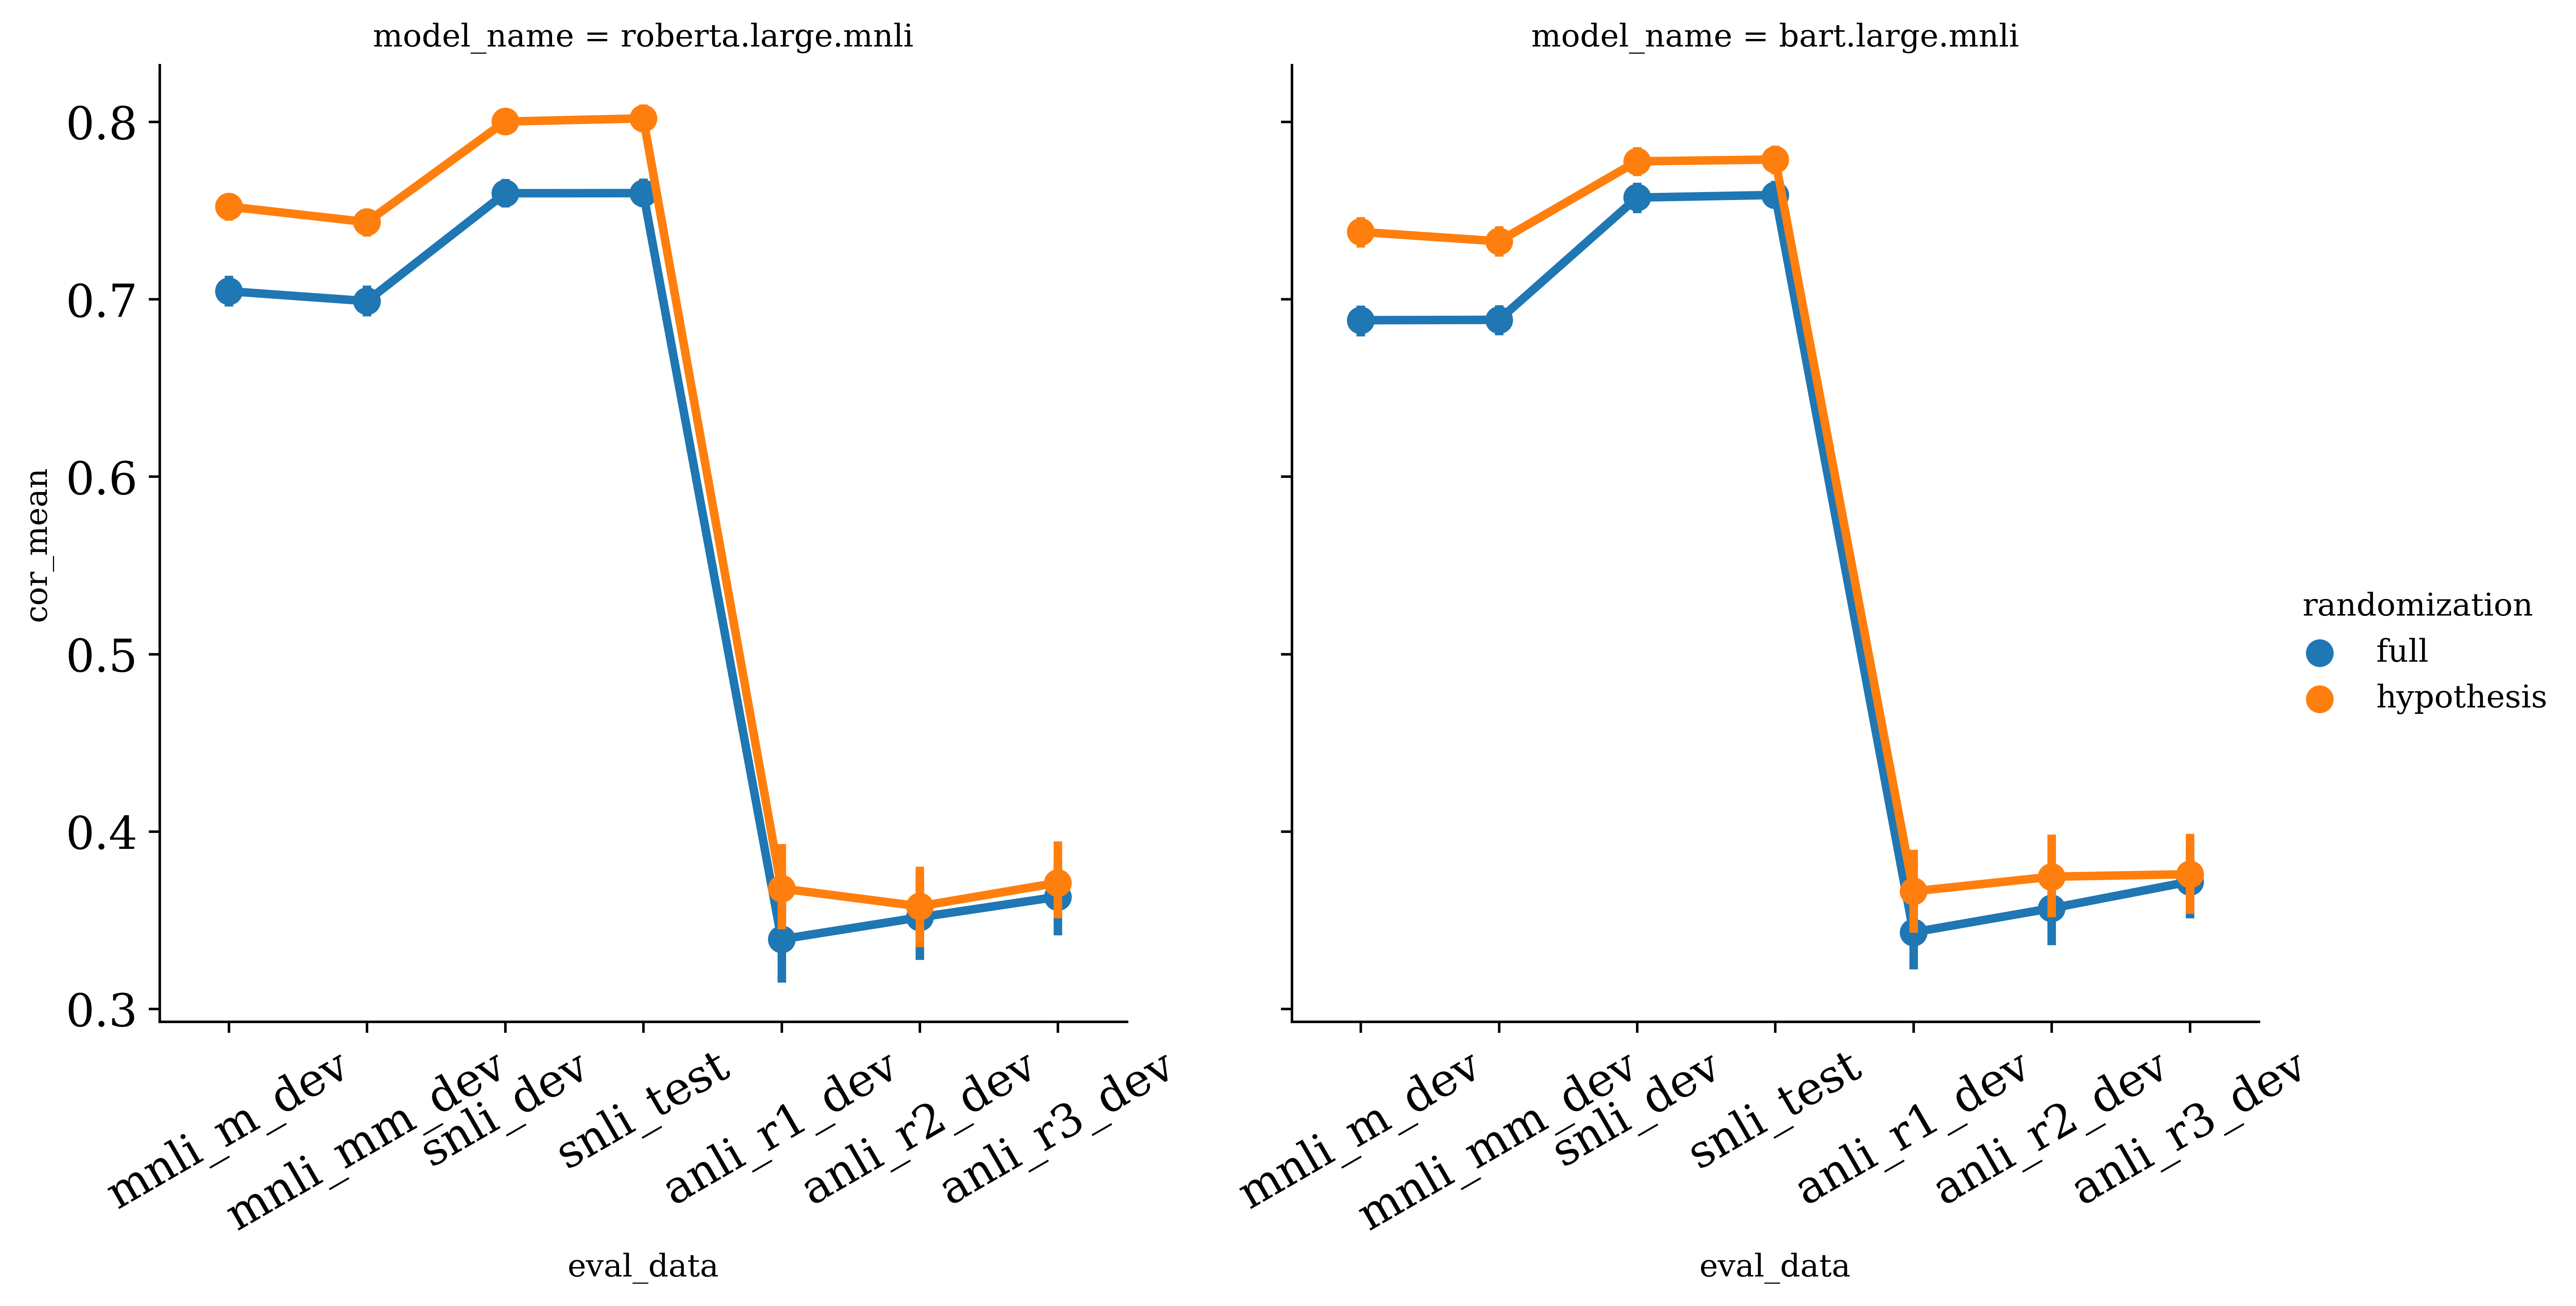
\includegraphics{figs/unli/hypothesis_compare_cor_mean.png}
      % \includegraphics{example-image-c}
    }
    \caption{Comparing the effect between randomizing both premise and hypothesis and only hypothesis on two Transformer-based models, RoBERTa and BART. In this figure, we compare the mean number of permutations which elicited correct response, and naturally the hypothesis-only randomization causes more percentage of randomizations to be correct.}
    \label{fig:unli_hp_compare_cor}
\end{figure}


In recent years, the impact of the hypothesis sentence \citep{gururangan-etal-2018-annotation, tsuchiya-2018-performance, poliak-etal-2018-hypothesis} on NLI classification has been a topic of much interest. As we define in \autoref{sec:unli_technical_bg}, logical entailment can only be defined for pairs of propositions. We investigated one effect where we randomize only the hypothesis sentences while keeping the premise intact. \autoref{fig:unli_hp_compare} and \autoref{fig:unli_hp_compare_cor} shows that the $\Omega_{\text{max}}$ value is almost the same for the two schemes; randomizing the hypothesis alone also leads the model to accept many permutations.


\section{Analysis}

\subsection{Analyzing Syntactic Structure Associated with Tokens}
\label{sec:unli_pos_mini_tree}


\begin{figure}[t]
    \centering
    \resizebox{0.48\textwidth}{!}{
        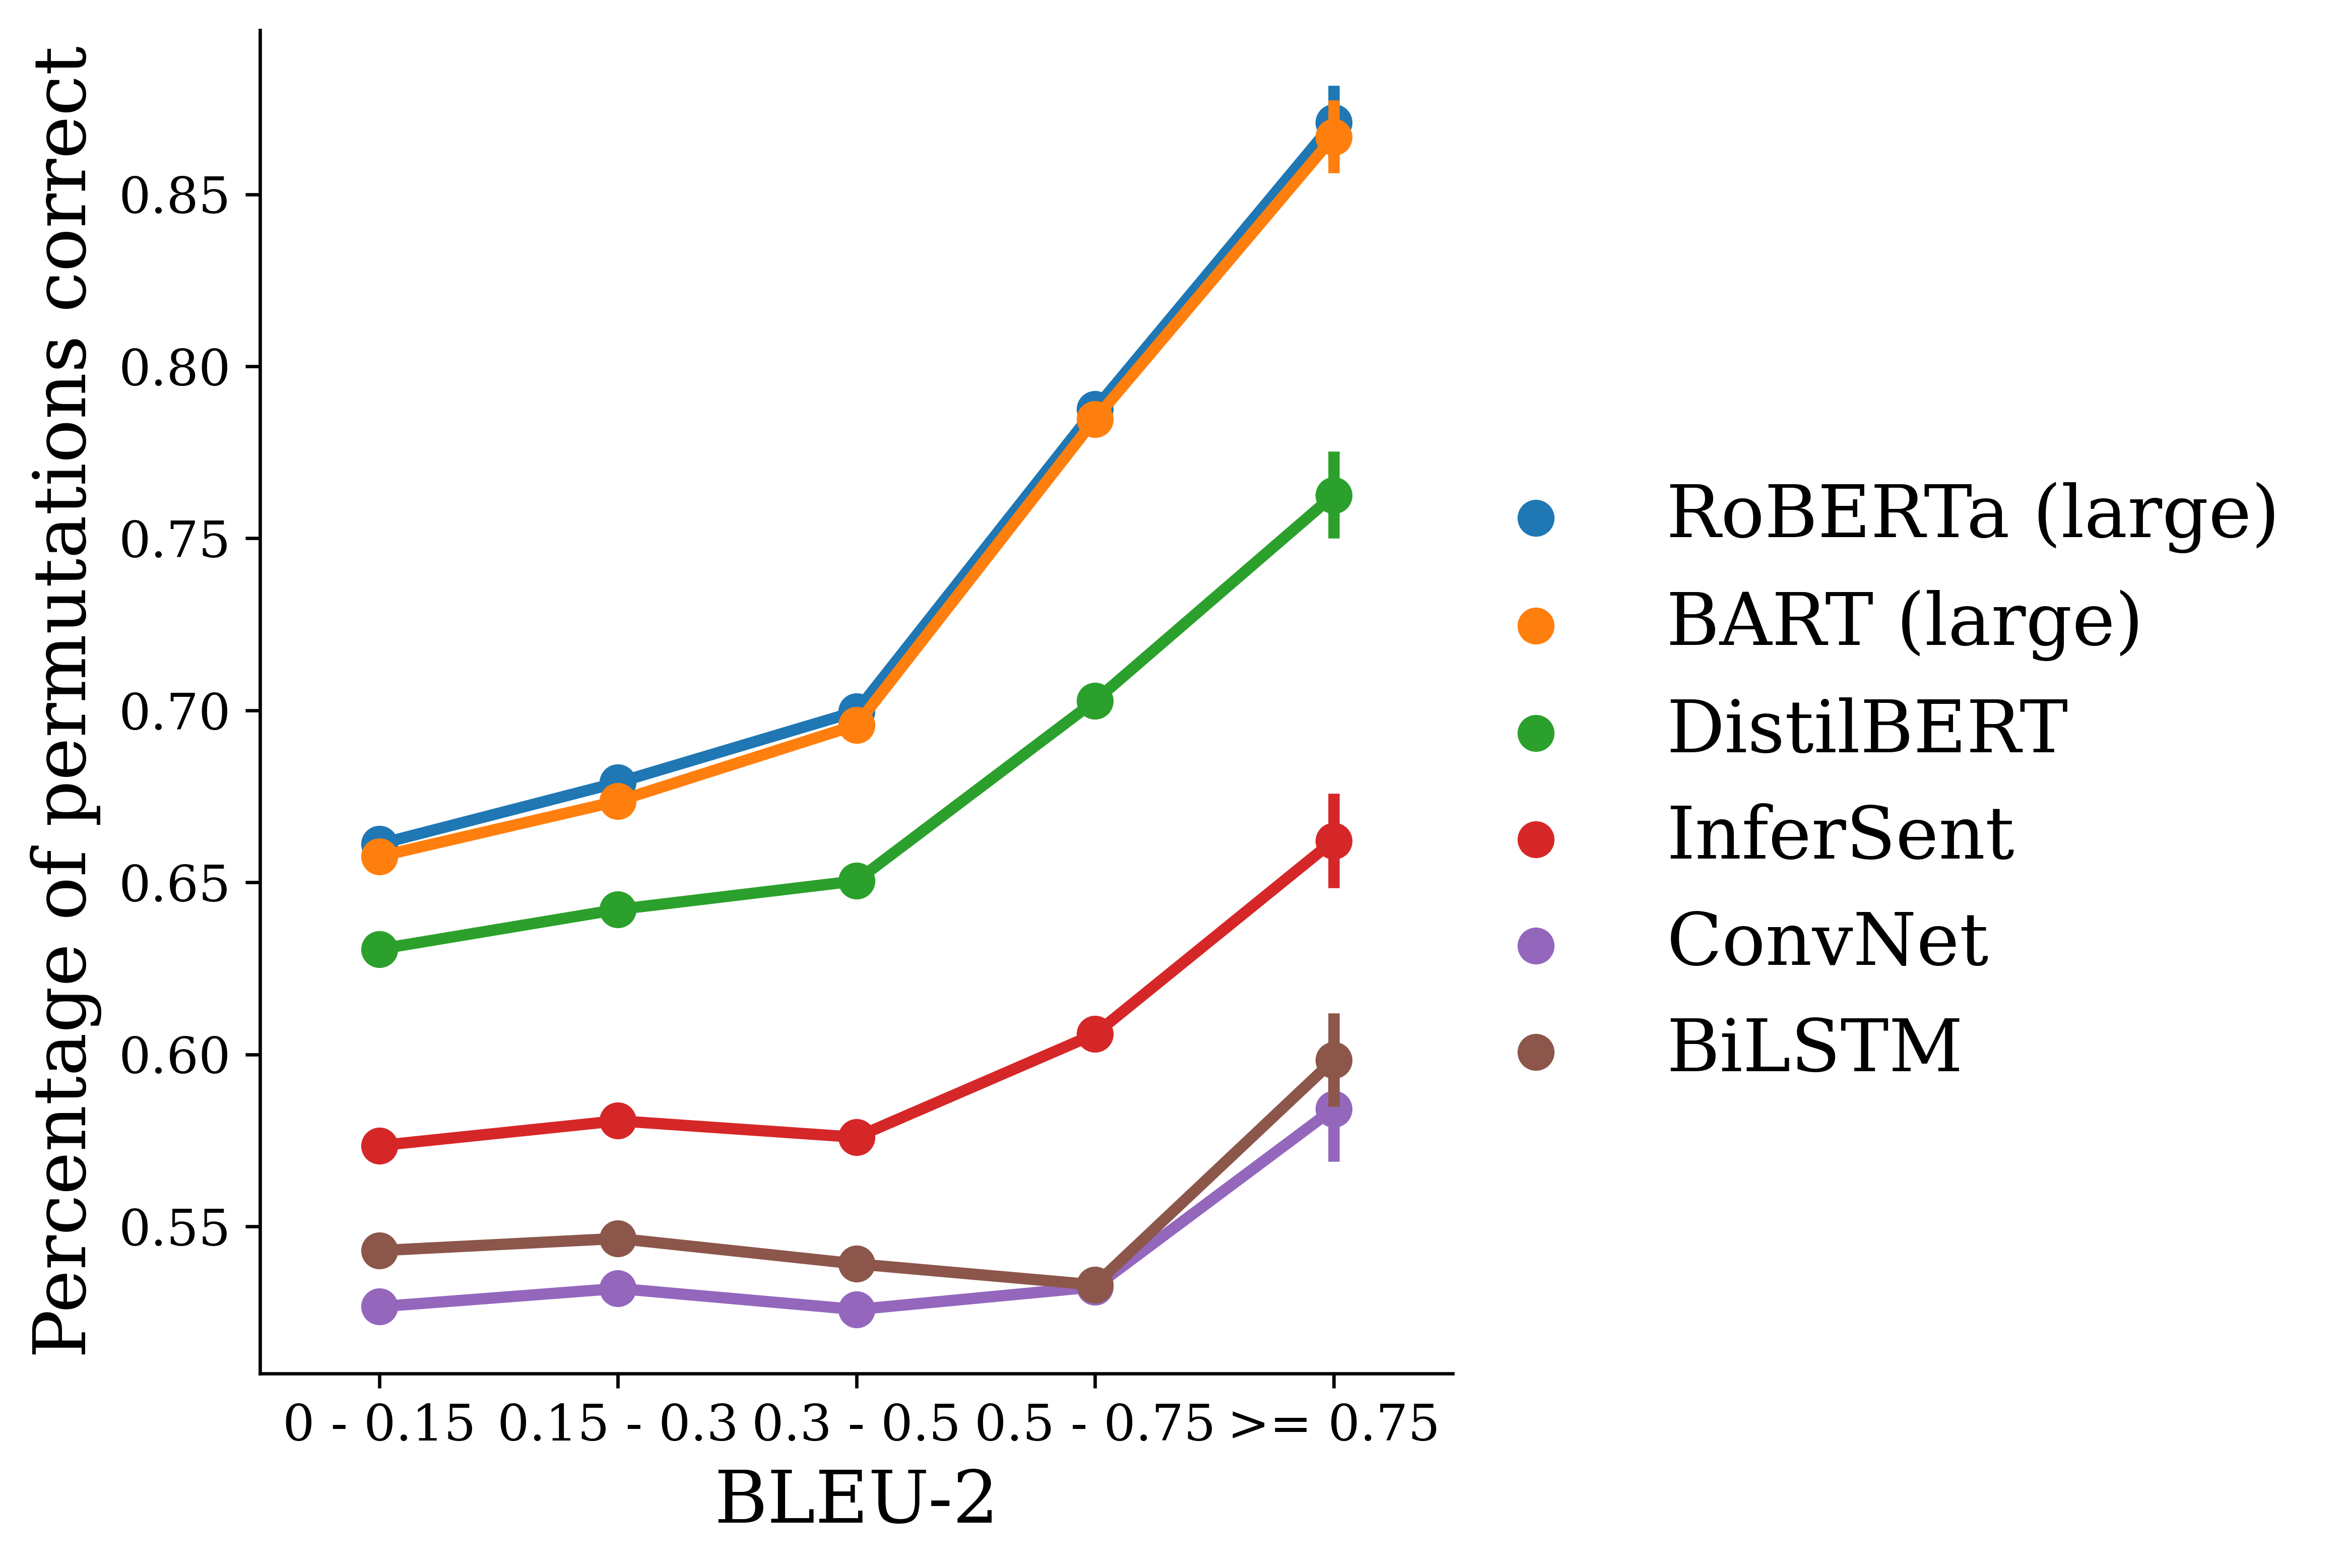
\includegraphics{figs/unli/bleu_2_all.png}}
    \caption{BLEU-2 score versus acceptability of permuted sentences across all test datasets. RoBERTa and BART performance is similar but differs considerably from the performance of non-Transformer-based models, such as InferSent and ConvNet. }
    \label{fig:bleu_2}
\end{figure}

A natural question to ask following our findings: what is it about particular permutations that leads models to accept them? Since the permutation operation is drastic and only rarely preserves local word relations, we first investigate whether there exists a relationship between \PermAcc\ scores and local word order preservation. Concretely, we compare bi-gram word overlap (BLEU-2) with the percentage of permutations that are deemed correct (\autoref{fig:bleu_2}).\footnote{We observe, due to our permutation process, the maximum BLEU-3 and BLEU-4 scores are negligibly low ($< 0.2$  BLEU-3 and $< 0.1$ BLEU-4), already calling into question the hypothesis that n-grams are the sole explanation for our finding. Because of this, we only compare BLEU-2 scores.} Although the probability of a permuted sentence to be predicted correctly does appear to track BLEU-2 score (Figure \ref{fig:bleu_2}), the percentage of examples which were assigned the gold label by the Transformer-based models is still higher than we would expect from permutations with lower BLEU-2 (66\% for the lowest BLEU-2 range of $0-0.15$), suggesting preserved relative word order alone cannot explain the high permutation acceptance rates.

Thus, we find that local order preservation does correlate with \PermAcc, but it doesn't fully explain the high \PermAcc\ scores.
We now further ask whether $\Omega$ is related to a more abstract measure of local word relations, i.e., part-of-speech (POS) neighborhood.

%We perform two initial analyses to shed light on this question. First, we ask whether \PermAcc\ scores are higher when local word order is preserved?
%We might expect this to be the case if the models memorize words along with their local neighbors. %does this clarify the point?
%We find that local order preservation does correlate with \PermAcc, but it doesn't fully explain the high \PermAcc\ scores. Second, we ask whether $\Omega$ is related to a more abstract measure of local word relations, i.e., part-of-speech (POS) neighborhood. We find that there is little effect of POS-neighbors for non-Transformer models, but that RoBERTa, BART, and DistilBERT show a distinct effect. Taken together these analyses suggest that some local word order information affects models' \PermAcc\ scores, and perhaps incorporating methods of decreasing model reliance on this information could be fruitful.

%\paragraph{Preserving Local Word Order Leads to Higher \PermAcc.}

%Although we constrained our randomization such that no word appears in its original position, we didn't impose any restrictions on the relative positions of n-grams. To investigate the extent to which relative n-gram order is preserved, we compare 2-, 3- and 4 n-gram BLEU scores \citep{papineni-etal-2002-bleu} to the $\Omega$ values across models.
%If preserved n-grams are driving the \PermAcc\ effects, we should low $\Omega$ values for examples with low BLEU and high $\Omega$ for examples with high BLEU. % didn't understand this part
%As a result of our permutation process, the maximum BLEU-3 and BLEU-4 scores are negligibly low ($< 0.2$  BLEU-3 and $< 0.1$ BLEU-4), already calling into question the hypothesis that n-grams are the sole explanation for our finding. Because of this, we only compare BLEU-2 scores. (Detailed experiments on specially constructed permutations that cover the entire range of BLEU-3 and BLEU-4 is provided in \autoref{app_sec:bleu_all}). Although the probability of a permuted sentence to be predicted correctly does correlate with BLEU-2 score (Figure \ref{fig:bleu_2}), the percentage of examples predicted correct by Transformer-based models is still higher than we would expect from permutations with lower BLEU-2 (66\% for the lowest BLEU-2 range of $0-0.15$), suggesting preserved relative word order alone cannot explain the high permutation acceptance rates.



% \paragraph{Part-of-speech neighborhood tracks \PermAcc.}

Many syntactic formalisms, like Lexical Functional Grammar \citep[LFG]{kaplan-bresnan-1995-formal, bresnan-etal-2015-lexical}, Head-drive Phrase Structure Grammar \citep[HPSG]{pollard-sag-1994-head} or Lexicalized Tree Adjoining Grammar \citep[LTAG]{schabes-etal-1988-parsing, abeille-1990-lexical}, are ``lexicalized'', i.e., individual words or morphemes bear syntactic features telling us which other words they can combine with. For example, ``buy'' could be associated with (at least) two lexicalized syntactic structures, one containing two noun phrases (as in \textit{\underline{Kim} bought \underline{cheese}}), and another with three (as in \textit{\underline{Lee} bought \underline{Logan} \underline{cheese}}). %In this way, an average tree family for any particular word, like \textit{buy}, can provide information about neighbors it often appears with. Taking inspiration from formalisms like this,
We speculate that our NLI models might accept permuted examples at high rates, %even when local n-gram orders aren't preserved,
because they are (perhaps noisily) reconstructing the original sentence from abstract, word-anchored information about common neighbors.

To test this, we POS-tagged $D_{\text{train}}$ using 17 Universal Part-of-Speech tags (using spaCy, \citealt{spacy}). %For each token in $D_{\text{train}}$, we get a summary of that token's syntactic context (at a symmetrical distance set by a hyperparameter we call the \textbf{radius}). Concretely,
For each $w_i \in S_i$, we compute the occurrence probability of POS tags on tokens in the \textit{neighborhood} of $w_i$. The neighborhood is specified by the radius $r$ (a symmetrical window $r$ tokens from $w_i \in S_i$ to the left and right). We denote this sentence level probability of neighbor POS tags for a word $w_i$ as $\psi^r_{\{w_i, S_i\}} \in \mathcal{R}^{17}$. Sentence-level word POS neighbor scores can be averaged across $ D_{\text{train}}$ to get a type level score $\psi^r_{\{w_i, D_{\text{train}}\}} \in \mathcal{R}^{17}, \forall w_i \in D_{\text{train}}$.  Then, for a sentence $S_i \in D_{\text{test}}$, for each word $w_i \in S_i$, we compute a \textbf{POS mini-tree overlap score}:
%\begin{align}
\begin{equation} % want left align
\begin{split}
\beta^k_{\{w_i,S_i\}} =
\frac{1}{k} \mid \text{argmax}_k &\psi^r_{\{w_i, D_{\text{train}}\}} \cap \\ &\text{argmax}_k\psi^r_{\{w_i, S_i\}} \mid
\end{split}
\end{equation}
%\end{align}

% POS signature?
Concretely, $\beta^k_{\{w_i,S_i\}}$ computes the overlap of top-$k$ POS tags in the neighborhood of a word $w_i$ in $S$ with that of the train statistic. If a word has the same mini-tree in a given sentence as it has in the training set, then the overlap would be 1. For a given sentence $S_i$, the aggregate $\beta^k_{\{S_i\}}$ is defined by the average of the overlap scores of all its words: $\beta^k_{\{S_i\}} = \frac{1}{|S_i|}\sum_{w_i \in S_i} \beta^k_{\{w_i,S_i\}}$, and we call it a POS minitree \textit{signature}. We can also compute the POS minitree signature of a permuted sentence $\hat{S}_i$ to have $\beta^k_{\{\hat{S}_i\}}$.  If the permuted sentence POS signature comes close to that of the true sentence, then their ratio (i.e.,  $\beta^k_{\{\hat{S}_i\}} / \beta^k_{\{S_i\}}$) will be close to 1. Also, since POS signature is computed with respect to the train distribution, a ratio of $>$ 1 indicates that the permuted sentence is closer to the overall train statistic than to the original unpermuted sentence in terms of POS signature. %If models ``know syntax'' then for any samples (from the permuted test set or from the original training) that have high average (?) POS tag minitree overlap scores (i.e., words with POS tag minitree scores similar to their POS tag minitree overlap score on the training set), we should expect those samples to be fairly easy for models to do well on.
If high overlap with the training distribution correlates with percentage of permutations deemed correct, then our models treat words as if they project syntactic minitrees.
%Therefore, for $\hat{D}_{\text{test}}$ where many of the $n$ permutations have high average POS minitree overlap score, we should expect a higher prediction accuracy.
\autoref{fig:unli_pos_signature} provides a snapshot a word ``river" from the test set and shows how the POS signature distribution of the word in a particular example match with that of aggregated training statistic. In practice, we select the top $k$ POS tags for the word in the test signature as well as the train, and calculate their overlap. When comparing the model performance with permuted sentences, we compute a ratio between the original test overlap score and an overlap score calculated instead from the permuted test. In the \autoref{fig:unli_pos_signature}, `river' would have a POS tag minitree score of 0.75.

\begin{figure}[ht]
    \centering
    \resizebox{0.7\linewidth}{!}{
        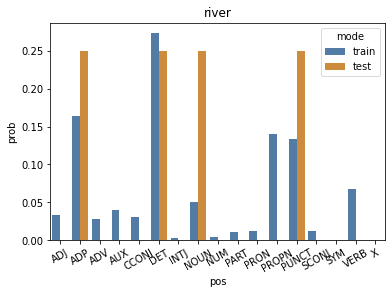
\includegraphics{figs/unli/riverPOSsig}}
    \caption{Example POS signature for the word `river', calculated with a radius of 2. Probability of each neighbor POS tag is provided. Orange examples come from the permuted test set, and blue come from the original training data. }
    \label{fig:unli_pos_signature}
\end{figure}



\begin{figure}[t]
    \centering
    \resizebox{0.6\linewidth}{!}{
        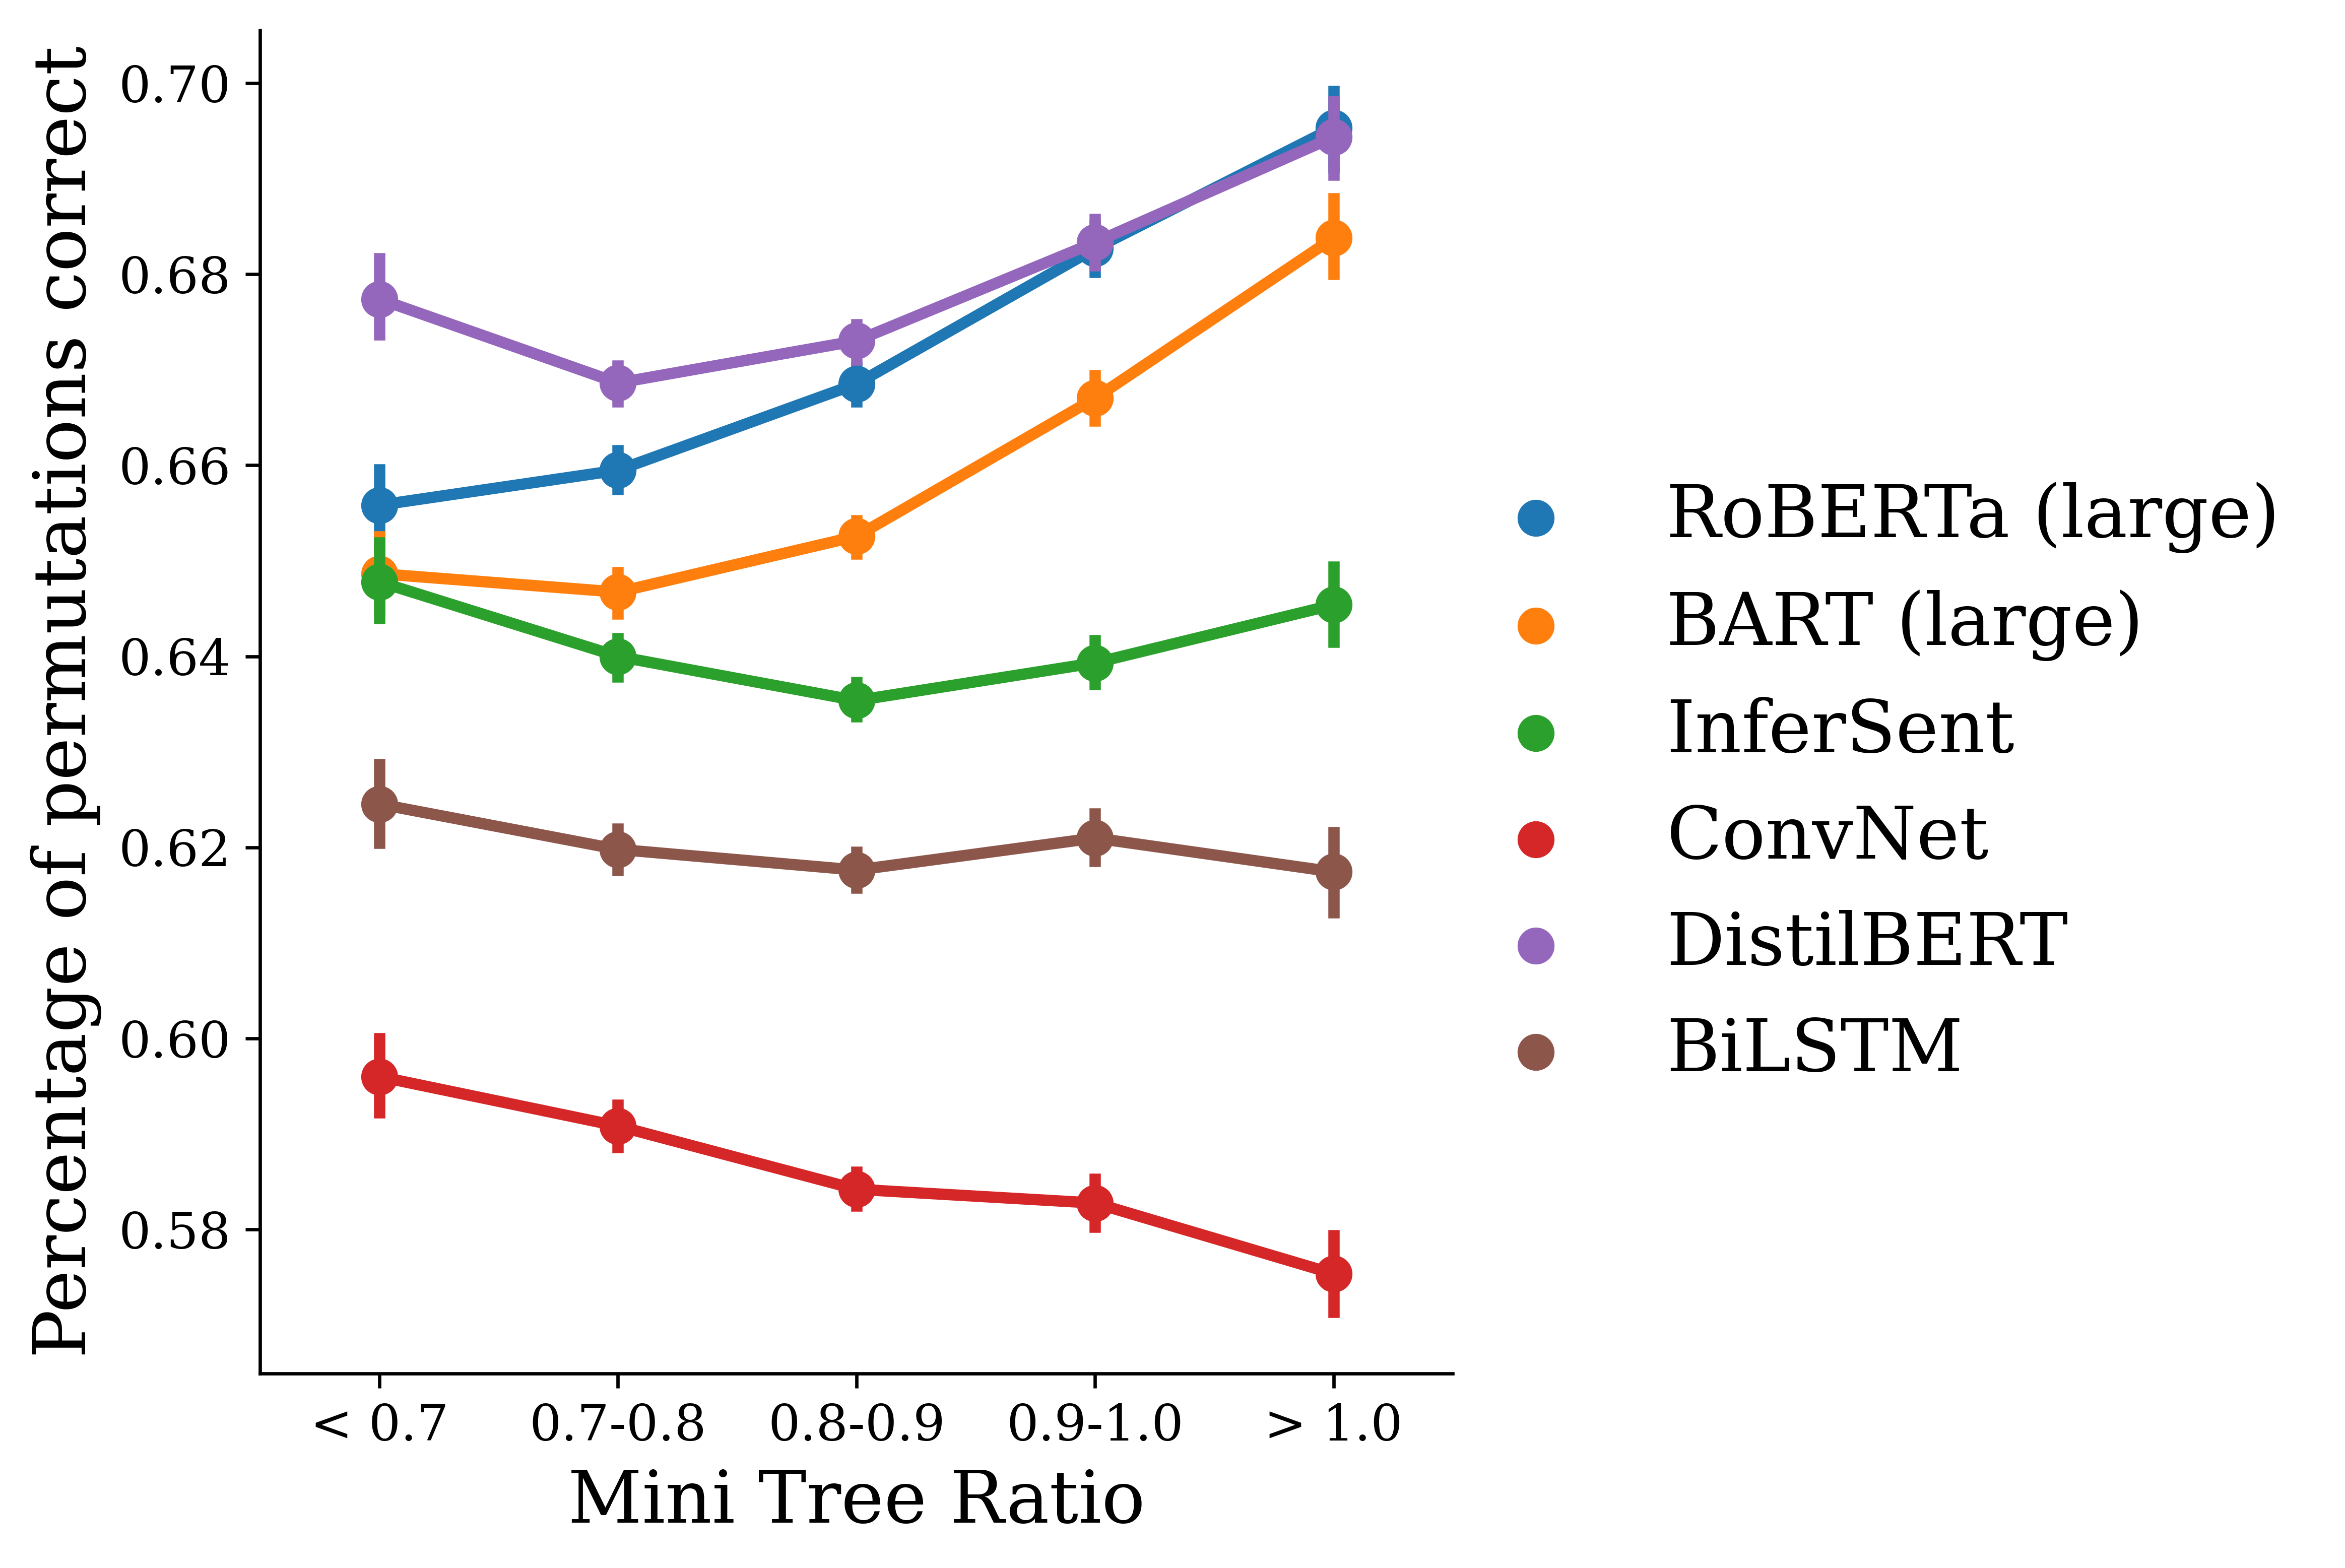
\includegraphics{figs/unli/min_tree_4.png}}
    \caption{POS Tag Mini Tree overlap score and  percentage of permutations which the models assigned the gold-label.}
    \label{fig:min_tree_4}
\end{figure}

We investigate the relationship with percentage of permuted sentences accepted with $\beta^k_{\{\hat{S}_i\}} / \beta^k_{\{S_i\}}$ in \autoref{fig:min_tree_4}. We observe that the POS Tag Minitree hypothesis holds for Transformer-based models, RoBERTa, BART and DistilBERT, where the percentage of accepted pairs increase as the sentences have higher overlap with the un-permuted sentence in terms of POS signature. For non-Transformer models such as InferSent, ConvNet, and BiLSTM models, the POS signature ratio to percentage of correct permutation remains the same or decreases, suggesting that the reasoning process employed by these models does not preserve local abstract syntax structure (i.e., POS neighbor relations).

%KS: Ideas: should we show POS tag correlation with original un-permuted sentences as well?

\subsection{Human Evaluation}
\label{sec:unli_human_eval}

%Since our models often accept permuted sentences, we ask how humans perform unnatural language inference on permuted sentences.
We expect humans to struggle with UNLI, given our intuitions and the sentence superiority findings (but see \citealt{mollica-2020-composition}). To test this, we presented two experts in NLI (one a linguist) with permuted sentence pairs to label.\footnote{Concurrent work by \cite{gupta-etal-2021-bert} found that untrained crowdworkers accept NLI examples that have been subjected to different kinds of perturbations at roughly most frequent class levels---i.e., only 35\% of the time.} Concretely, we draw equal number of examples from MNLI Matched dev set (100 examples where RoBERTa predicts the gold label, $D^c$ and 100 examples where it fails to do so, $D^f$), and then permute these examples using $\mathcal{F}$. The experts were given no additional information (recall that it is common knowledge that NLI is a roughly balanced 3-way classification task). Unbeknownst to the experts, all permuted sentences in the sample were actually accepted by the RoBERTa (large) model (trained on MNLI dataset). We observe that the experts performed much worse than RoBERTa (\autoref{tab:human_eval}), although their accuracy was a bit higher than random. We also find that for both experts, accuracy on permutations from $D^c$ was higher than on $D^f$, which verifies findings that showed high word overlap can give hints about the ground truth label \citep{dasgupta-etal-2018-evaluating, poliak-etal-2018-hypothesis, gururangan-etal-2018-annotation, naik-etal-2019-exploring}.

% Please add the following required packages to your document preamble:
% \usepackage{booktabs}
% \usepackage{graphicx}
\begin{table}[t]
\centering
\resizebox{0.7\linewidth}{!}{%
\begin{tabular}{@{}lllll@{}}
\toprule
Evaluator & Accuracy & Macro F1 & Acc on $D^{c}$ & Acc on $D^{f}$ \\ \midrule
X & 0.581 $\tiny\pm 0.068$ & 0.454 & 0.649 $\tiny\pm 0.102$ & 0.515 $\tiny\pm 0.089$ \\
Y &  0.378 $\tiny\pm 0.064$ & 0.378 & 0.411 $\tiny\pm 0.098$ & 0.349 $\tiny\pm 0.087$ \\ %\midrule
%crowd^{*} & & 0.35 & \\
\bottomrule
\end{tabular}%
}
\caption{Human (expert) evaluation on 200 permuted examples from the MNLI matched development set. Half of the permuted pairs contained shorter sentences and the other, longer ones. %Experts were provided only the permuted sentences (not the original example or the label) and were disallowed from consulting with one another. 
All permuted examples were assigned the gold label by RoBERTa-Large. %crowd$^*$ was crowdworker accuracy measured by \newcite{gupta-etal-2021-bert} on the GLUE Benchmark. 
}
\label{tab:human_eval}
\end{table}


\subsection{Training by Maximizing Entropy}
\label{sec:unli_training}
% training done on roberta.large.

We propose an initial attempt to mitigate the effect of correct prediction on permuted examples. As we observe in \autoref{sec:unli_results_conf}, model entropy on permuted examples is significantly lower than expected.
%This kind of phenomenon has been observed prior in Computer Vision \cite{gandhi2019mutual}, and suggests model struggle to to learn \textit{mutually exclusively}.
Neural networks tend to output higher confidence than random for even unknown inputs \cite{gandhi2019mutual}, which might be an underlying cause of the high \PermAcc.

% \begin{figure}
%     \centering
%     \resizebox{\linewidth}{!}{
%         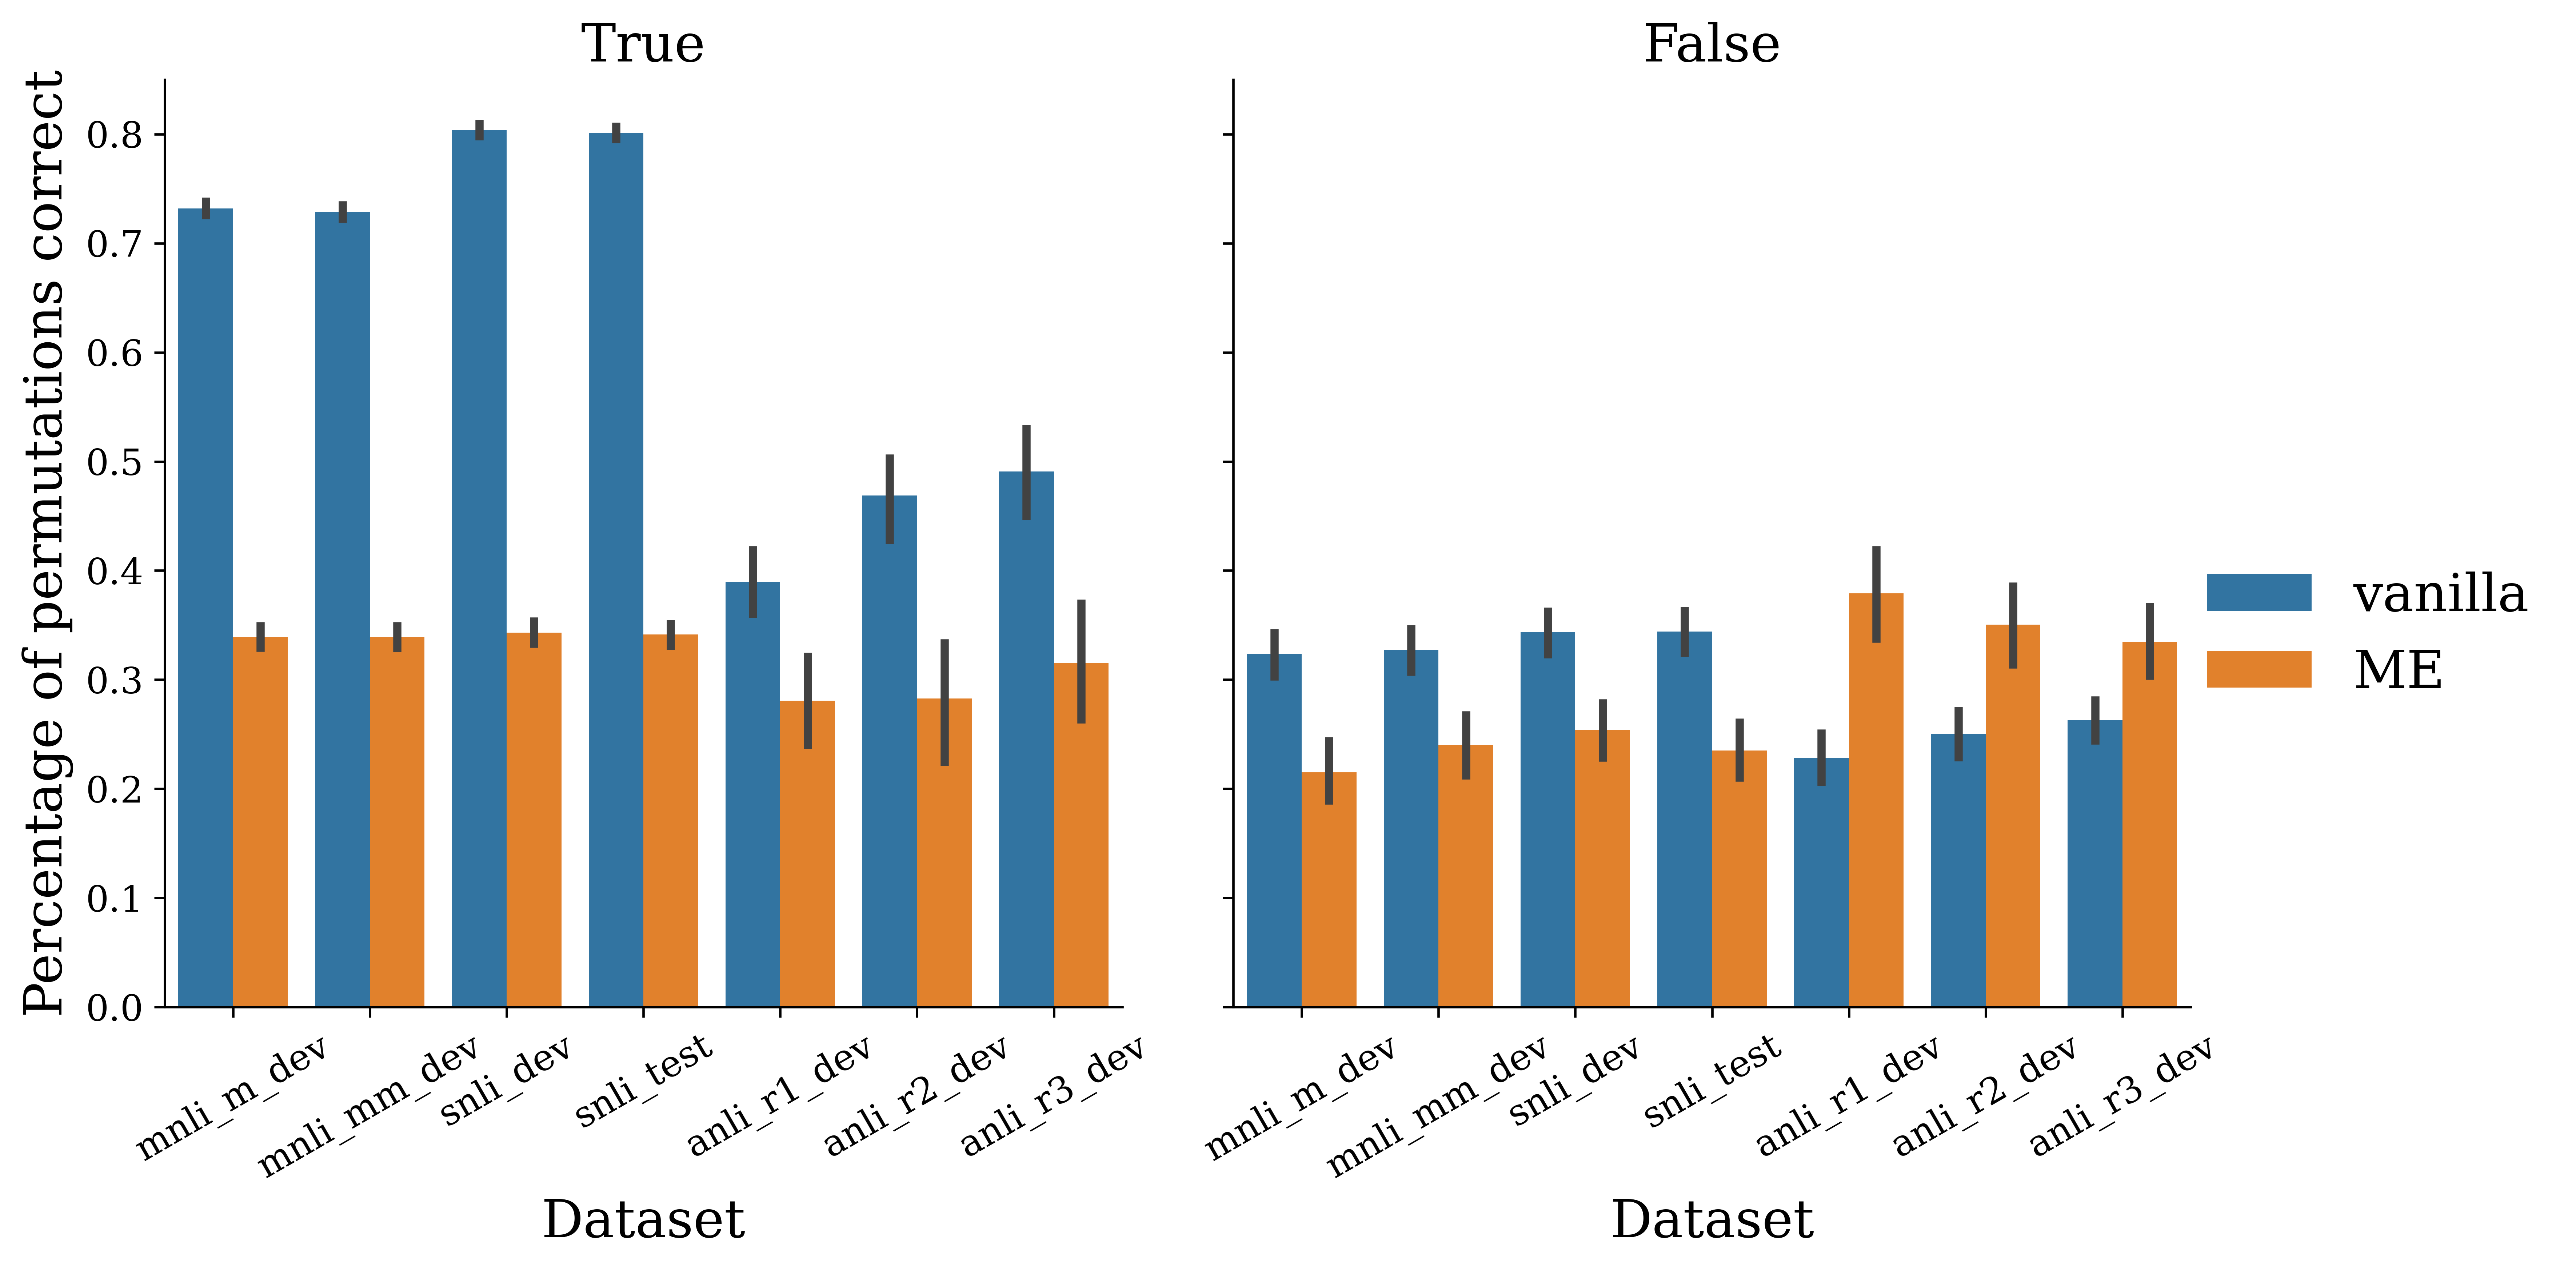
\includegraphics{images/me_train_roberta.png}}
%     \caption{Effect of maximizing entropy training on RoBERTa (large)}
%     \label{fig:max_ent_roberta}
% \end{figure.}

An ideal model would be ambivalent about randomized ungrammatical sentences. Thus, we train NLI models baking in the principle of mutual exclusivity \citep{gandhi2019mutual} by maximizing model entropy. Concretely, we fine-tune RoBERTa on MNLI while maximizing the entropy ($\bm{\mathcal{H}}$) on a subset of $n$ randomized examples ($(\hat{p}_i, \hat{r}_i$), for each example ($p,h$) in MNLI. We modify the loss function as follows:
% Prasanna
\begin{dmath}
    \mathcal{L}=\argminB_{\theta}\sum_{\left((p, h),y\right)}y\log(p(y|(p,h);\theta)) + \sum_{i=1}^n \bm{\mathcal{H}}\left(y|(\hat{p}_i,\hat{h}_i);\theta\right)
\end{dmath}
Using this maximum entropy method ($n=1$), we find that the model improves considerably with respect to its robustness to randomized sentences, all while taking no hit to accuracy (\autoref{table:ME_train_roberta}). We observe that no model reaches a $\Omega_{\text{max}}$ score close to 0, suggesting further room to explore other methods for decreasing models' \PermAcc. Similar approaches have also proven useful \citep{gupta-etal-2021-bert} for other tasks as well.

\begin{table}[t]
\centering
\resizebox{0.7\linewidth}{!}{%
\begin{tabular}{lrrrr}
\toprule
   Eval Dataset &   $\mathcal{A}$ (V) &  $\mathcal{A}$ (ME) &  $\Omega_{\text{max}}$ (V) &  $\Omega_{\text{max}}$ (ME) \\
\midrule
  MNLI\_m\_dev &  0.905 &     0.908 &    0.984 &        0.328 \\
 MNLI\_mm\_dev &  0.901 &     0.903 &    0.985 &        0.329 \\
   SNLI\_test &  0.882 &     0.888 &    0.983 &        0.329 \\
    SNLI\_dev &  0.879 &     0.887 &    0.984 &        0.333 \\
 ANLI\_r1\_dev &  0.456 &     0.470 &    0.890 &        0.333 \\
 ANLI\_r2\_dev &  0.271 &     0.258 &    0.880 &        0.333 \\
 ANLI\_r3\_dev &  0.268 &     0.243 &    0.892 &        0.334 \\
\bottomrule
\end{tabular}}
\caption{NLI Accuracy ($\mathcal{A}$) and \PermAcc\ metrics ($\Omega_{\text{max}}$) of RoBERTa when trained on MNLI dataset using vanilla (V) and Maximum Random Entropy (ME) method.}
  \label{table:ME_train_roberta}
\end{table}





\section{Related Work}
\label{sec:unli_related}

Researchers in NLP have realized the importance of syntactic structure in neural networks going back to \cite{tabor-1994-syntactic}. An early hand annotation effort on PASCAL RTE \citep{dagan-etal-2006} suggested that ``syntactic information alone was sufficient to make a judgment'' for roughly one third of examples %, whereas almost a half could be solved if annotators were additionally provided a thesaurus
\citep{vanderwende2005syntax}. %
Anecdotally, large generative language models like GPT-2 or -3 exhibit a seemingly humanlike ability to generate fluent and grammatical text \citep{goldberg2019assessing, wolf2019some}.
However, the jury is still out as to whether transformers genuinely acquire syntax.

\subsection{Models appear to have acquired syntax.}

When researchers have peeked inside Transformer LM's pretrained representations, familiar syntactic structure \citep{hewitt-manning-2019-structural,jawahar-etal-2019-bert, lin-etal-2019-open, warstadt-bowman-2020-can, wu-etal-2020-perturbed}, or a familiar order of linguistic operations \citep{jawahar-etal-2019-bert,  tenney-etal-2019-bert}, has appeared. There is also evidence, notably from agreement attraction phenomena \citep{linzen-etal-2016-assessing} that transformer-based models pretrained on LM do acquire some knowledge of natural language syntax \citep{gulordava-etal-2018-colorless, chrupala-alishahi-2019-correlating,  jawahar-etal-2019-bert, lin-etal-2019-open, manning-etal-2020-emergent,  hawkins-etal-2020-investigating, linzen-baroni-2021-syntactic}. Results from other phenomena \citep{warstadt-bowman-2020-can} such as NPI licensing  \citep{warstadt-etal-2019-investigating} lend additional support. The claim that LMs acquire some syntactic knowledge has been made not only for transformers, but also for convolutional neural nets \citep{bernardy-lappin-2017-using}, and \acrshort{rnn}s \citep{gulordava-etal-2018-colorless, van-schijndel-linzen-2018-neural, wilcox-etal-2018-rnn, zhang-bowman-2018-language, prasad-etal-2019-using, ravfogel-etal-2019-studying}---although there are many caveats (e.g., \citealt{ravfogel-etal-2018-lstm, white-etal-2018-lexicosyntactic,  davis-van-schijndel-2020-recurrent, chaves-2020-dont, da-costa-chaves-2020-assessing, kodner-gupta-2020-overestimation}).

\subsection{Models appear to struggle with syntax.}

Several works have cast doubt on the extent to which NLI models in particular know syntax (although each work adopts a slightly different idea of what ``knowing syntax'' entails). For example, \cite{mccoy-etal-2019-right} argued that the knowledge acquired by models trained on NLI (for at least some popular datasets) is actually not as syntactically sophisticated as it might have initially seemed; some transformer models rely mainly on simpler, non-humanlike heuristics. In general, transformer LM performance has been found to be patchy and variable across linguistic phenomena \citep{dasgupta-etal-2018-evaluating, naik-etal-2018-stress, an-etal-2019-representation, ravichander-etal-2019-equate, jeretic-etal-2020-natural}. This is especially true for syntactic phenomena \citep{marvin-linzen-2018-targeted, hu-etal-2020-systematic, gauthier-etal-2020-syntaxgym, mccoy-etal-2020-berts, warstadt-etal-2020-blimp}, where transformers are, for some phenomena and settings, worse than \acrshort{rnn}s \citep{van-schijndel-etal-2019-quantity}. From another angle, many have explored architectural approaches for increasing a network's sensitivity to syntactic structure \citep{chen-etal-2017-enhanced, Li-etal-2020-SANLI}. \cite{williams-etal-2018-latent} showed that learning jointly to perform NLI  and to parse resulted in parse trees that match no popular syntactic formalisms. Furthermore, models trained explicitly to differentiate acceptable sentences from unacceptable ones (i.e., one of the most common syntactic tests used by linguists) have, to date, come nowhere near human performance \citep{warstadt-etal-2019-neural}.

\subsection{Insensitivity to Perturbation.}

Most relatedly, several concurrent works \citep{pham-etal-2020-out, alleman2021syntactic, gupta-etal-2021-bert, sinha-etal-2021-masked,parthasarathi-etal-2021-sometimes-want} investigated the effect of word order permutations on transformer NNs.  \cite{pham-etal-2020-out} is very nearly a proper subset of our work except for investigating additional tasks (i.e. from the GLUE benchmark of \citealt{wang-etal-2018-glue}) and performing a by-layer-analysis. \cite{gupta-etal-2021-bert} also relies on the GLUE benchmark, but additionally investigates other types of ``destructive'' perturbations. Our contribution differs from these works %, although our tentative Maximum Entropy solution parallels a similar one in \newcite{}
in that we additionally include the following: we (i) outline theoretically-informed predictions for how models \emph{should be expected} to react to permuted input (we outline a few options), (ii) show that permuting can ``flip'' an incorrect prediction to a correct one, (iii) show that the problem isn't specific to Transformers, (iv) show that the problem persists on out of domain data, (v) offer a suite of flexible metrics, and (vi) analyze \emph{why} models might be accepting permutations (BLEU and POS-tag neighborhood analysis). Finally, we replicate our findings in another language.
% cite our two permutations papers & Yoon's student's in relation to our translation paper.
While our work (and \citeauthor{pham-etal-2020-out,gupta-etal-2021-bert}) only permutes data during fine-tuning and/or evaluation,
%raising the natural question: what is the result of permuting during training. \newcite{sinha-etal-2021-masked} addresses this question.
recently \citeauthor{sinha-etal-2021-masked} explored the sensitivity during pre-training, and found that models trained on n-gram permuted sentences perform remarkably close to regular \acrshort{mlm} pre-training.
In the context of generation, \cite{parthasarathi-etal-2021-sometimes-want} crafted linguistically relevant perturbations (on the basis of part-of-speech tagging and dependency parsing) to evaluate whether permutation hinders automatic machine translation models. Relatedly, but not for translation, \cite{alleman2021syntactic} investigated a smaller inventory of perturbations with emphasis on phrasal boundaries and the effects of n-gram perturbations on different layers in the network. % AW: Koustuv, please check this

% TODO: gururangan citation is double, check and remove

\subsection{NLI Models are very sensitive to words.}

NLI models often over-attend to particular words to predict the correct answer \citep{gururangan-etal-2018-annotation, clark-etal-2019-bert}. \cite{wallace-etal-2019-universal} show that some short sequences of non-human-readable text can fool many \acrshort{nlu} models, including NLI models trained on SNLI, into predicting a specific label. In fact, \cite{ettinger-2020-whatbertisnot} observed that for one of three test sets, BERT loses some accuracy in word-perturbed sentences, but that there exists a subset of examples for which BERT’s accuracy remains intact.
%This led \citeauthor{ettinger-2020-whatbertisnot} to speculate that ``some of BERT's success on these items may be attributable to simpler lexical or n-gram information''. Thus, it is reasonable to wonder how well NLI models will perform on permuted sentences where the model is able to view the same collection of words.
If performance isn't affected (or if permutation helps, as we find it does in some cases), it suggests that these state-of-the-art models actually perform somewhat similarly to bag-of-words models \cite{blei-etal-2003-latent, mikolov2013efficient}.

% Todo: cite dasgupta et al
% Todo: cite goodwin et al



\section{Discussion}
\label{sec:unli_discussion}

In this chapter, we observe that state-of-the-art models do not rely on sentence structure the way we think they should: NLI models (Transformer-based models, \acrshort{rnn}s, and ConvNets) are largely insensitive to permutations of word order that corrupt the original syntax. This raises questions about the extent to which such systems understand ``syntax'', and highlights the unnatural language understanding processes they employ. To summarize, our primary observations from this chapter are:

\begin{itemize}
  \item \textbf{\acrshort{nlu} models can still perform the task even if the word orders are scrambled} We observed overwhelming evidence in \autoref{sec:unli_results_accept} that state-of-the-art \acrshort{nlu} models tend to perform the task comparably even on word order scrambled text, which has no inherent semantic meaning.

  \item \textbf{Certain permutations allow \acrshort{nlu} models to flip classification labels, leading to better task scores.} We find that certain permutations of the order of words in a given input sentence pair can trigger the model to change the classification labels from the baseline, leading to large performance gains in the scores of the NLI task. For instance, in the examples which the models find difficult to predict, a permutation of the word order can elicit the model to assign the gold label.

  \item \textbf{\acrshort{nlu} models display rudimentary understanding of syntax, as evident by the preservation of abstract parts-of-speech neighborhood information.} We do find that models seem to have learned some syntactic information as is evidenced by a correlation between preservation of abstract POS neighborhood information and rate of acceptance by models, but these results do not discount the high rates of \PermAcc, and require further verification.

\end{itemize}


%While we have shown that classification labels can be flipped based solely on a sentence reordering, on interesting future direction to explore might be to additionally consider dropping tokens. Such an approach has been taken in the realm of interpretability to determine the impact of particular tokens on model decisions \citep{serrano-smith-2019-attention}. %% COMMENT OUT ABOVE FOR ARXIV SUBMIT.
% We also observe that reordering words can cause models to flip classification labels. % future work could additionally explore the relationship between permutation and deletion.
Given these findings, and coupled with the observation that humans cannot perform UNLI at all well, the high rate of permutation acceptance that we observe leads us to conclude that current models do not yet ``know syntax'' in the fully systematic and humanlike way we would like them to. This study leads us to further investigate the training dynamics employed by these large language models. In the next chapter, we will investigate the training data dependency of one such model family in detail, to shed more light on the sentence processing pipelines employed by these models.

\section{Follow-up findings in the community}
\label{sec:unli_followup}

Our work in this chapter was among the first to discover the issue of word order permutation in the large language models. Concurrent to our publication, \citet{gupta-etal-2021-bert} and \citet{pham-etal-2020-out} also converge on similar findings on different \acrshort{nlu} datasets. Thus, our paper opened a new line of inquiry on the susceptibility of word order of language models, and in general encouraging the community to probe the cause of related systematicity issues displayed by these models.
\citet{hessel-schofield-2021-effective} arrive at similar conclusions on word-order invariance as demonstrated in our work in this chapter. The authors then further utilizes the phenomenon to develop privacy sensitive \acrshort{nlu} models which can operate on a bag-of-words representation of a document without losing task performance.
\citet{Malkin2021StudyingWO} also provide similar conclusions to our work, and they leverage the word-order invariance of Transformer-family of models to develop a new iterative shuffling inference mechanism to find out the most likely word order of a sentence according to a given model, and thereby demonstrate improvements to language modelling and generation.
\citet{perez2021} take inspiration from the word-order insensitivity results on Transformer models from our work to develop a novel method, Rissanen Data Analysis, to estimate the models learning ability by measuring the \acrfull{mdl}. \acrshort{mdl} captures the training behavior of the model during the initial stages of fine-tuning. The authors compute the \acrshort{mdl} on various downstream tasks with and without word order shuffling, to find that models display significantly different learning behavior on word order shuffles than on the normal mode \citep[Section 4.3.4, pp. 8.][]{Perez2021RissanenDA}. However, having different learning characteristics does not fully explain our results of word-order insensitivity, indicating the issue requires further study to find out the root cause.
\citet{parthasarathi-etal-2021-sometimes-want} extend our experimental setup to investigate how neural machine translation (NMT) systems translate ungrammatical, shuffled input sentences. They observe that state-of-the-art NMT models overwhelmingly \textit{fix} the ungrammaticality of the input in their translations, thereby exhibiting robust behavior.
\cite{clouatre-etal-2022-local} attempts to explain the word-order insensitivity issue of several types of neural models, including Transformer-family of models. They come to the conclusion that neural models across all types of inductive bias (i.e., including \acrshort{rnn}/LSTM/Transformer models) rely on local structure of text instead of the global structure to build the sentence representation, which also corroborates to our syntax structure hypothesis (\autoref{sec:unli_pos_mini_tree}).
\cite{websonPavlick2022} investigate the systematicity issues in prompt-based models, specifically to gain insights on whether high-performing prompt-based models understand the meaning of the said prompts. They find that despite the impressive zero/few-shot performance of massive language models such as GPT3 \citep{Brown2020:GPT3}, they lack proper systematic understanding capability of the provided prompts, so much so that they produce good predictions even with misleading and irrelevant prompts.
\citet{Tejankar2021AFO} leverage the word order insensitivity of Transformer models to develop a bag-of-words image captioning model which are trained on synthetically crafted bag-of-word captions. They achieve superior zero shot performance on ImageNet dataset by using 1/5th amount of image-caption pairs than the baseline model.
The following chapter is also a direct consequence of the results observed in this work.

\clearpage
\chapter{Probing syntax understanding through distributional hypothesis}
\label{sec:mlm}

The field of natural language processing (NLP) has become dominated by the pretrain-and-finetune paradigm, where we first obtain a good parametric \emph{prior} in order to subsequently model downstream tasks accurately.
In particular, masked language model (\acrshort{mlm}) pre-training, as epitomized by BERT \citep{devlin-etal-2019-bert}, has proven wildly successful, although the precise reason for this success has remained unclear.
On one hand, we can view BERT as the newest in a long line of NLP techniques  \citep{deerwester1990indexing, landauer1997solution, collobert2008unified, mikolov2013, peters-etal-2018-deep} that exploit the well-known distributional hypothesis~\citep{harris1954distributional}.
%\footnote{One might even argue that BERT is not actually all that different from earlier distributional models like word2vec~\cite{mikolov2013}, see \autoref{app:bert-is-word2vec}.}
On the other hand, it has been claimed that BERT ``rediscovers the classical NLP pipeline''~\citep{tenney-etal-2019-bert}, suggesting that it has learned ``the types of syntactic and semantic abstractions traditionally believed necessary for language processing''
rather than ``simply modeling complex co-occurrence statistics''~(ibid. p.1).

In this chapter, we aim to uncover how much of \acrshort{mlm}'s success comes from learning simple distributional information, as opposed to grammatical abstractions \citep{tenney-etal-2019-bert,manning-etal-2020-emergent}. Thus, in this chapter I discuss our work \citep{sinha-etal-2021-masked}, where we disentangle these two hypotheses by measuring the effect of removing word order information during pre-training:
any sophisticated (English) NLP pipeline would presumably depend on the syntactic information conveyed by the order of words.
We find that surprisingly most of \acrshort{mlm}'s high performance can in fact be explained by the ``distributional prior'' rather than its ability to replicate the classical NLP pipeline.

Concretely, we pre-train \acrshort{mlm}s~(RoBERTa, \citealt{liu-et-al-2019-roberta}) on various corpora with permuted word order while preserving some degree of distributional information, and examine their downstream performance.
%In our main experiments, we pre-train models on
%various permuted corpora , by randomly shuffling $n$-grams within the sentence (where $n \in \{1,2,3,4\}$).
We also experiment with training \acrshort{mlm}s without positional embeddings, making them entirely order agnostic,
and with training on a corpus sampled from the source corpus's %uniform or
unigram distribution%, removing both distributional and word order information
. We then evaluate these ``permuted'' models in a wide range of settings and compare with regularly-pre-trained models.

We demonstrate that pre-training on permuted data has surprisingly little effect on downstream task performance after fine-tuning (on non-shuffled training data).
In our previous chapter we observed that \acrshort{mlm}s are quite robust to permuting downstream test data (\autoref{sec:unli_results_accept}) and even do quite well using permuted ``unnatural'' downstream train data \citep{sinha-etal-2021-unnatural,gupta-etal-2021-bert}. In this chapter, we show that downstream performance for ``unnatural language pre-training'' is much closer to standard \acrshort{mlm} pre-training than one might expect.

In an effort to shed light on these findings, we experiment with various probing tasks. We verify via non-parametric probes that the permutations do in fact make the model worse at syntax-dependent tasks. However, just like on the downstream fine-tuning tasks, permuted models perform well on parametric syntactic probes, in some cases almost matching the unpermuted model's performance, which is quite surprising given how important word order is crosslinguistically (\citealt{greenberg1963some, dryer1992greenbergian, cinque1999adverbs}, i.a.).

Our results can be interpreted in different ways.
One could argue that our downstream and probing tasks are flawed, and that we need to examine models with examples that truly test strong generalization and compositionality.
Alternatively, one could argue that prior works have overstated the dependence of human language understanding on word order, and that human language understanding depends less on the structure of the sentence and more on the structure of the \emph{world}, which can be inferred to a large extent from distributional information.
This work is meant to deepen our understanding of \acrshort{mlm} pre-training and, through this, move us closer to finding out what is actually required for adequately modelling natural language.



\section{Technical Background}
\label{sec:mlm_bg}

Masked Language Modelling (\acrshort{mlm}) is a pre-training technique popularized by BERT \citep{devlin-etal-2019-bert}. Unlike the autoregressive processing of traditional Transformer \citep{vaswani-etal-2017-attention} models, BERT introduces bi-directional attention mechanism in which the model no longer have to restrict attentions to past tokens: the model can now attend to any tokens in the input, in both left-to-right and right-to-left directions (\autoref{sec:bg_pretraining}). To train such bi-directional self-attention models, \acrshort{mlm} pre-training is used where first the input sentence is corrupted by replacing 15\% of tokens with mask token (\texttt{<MASK>}), and then the training objective entails predicting the masked tokens in the output. Thus, to predict any mask token, the model can attend to the entire context (hence the bi-directionality). This kind of pre-training technique allows models to be trained in larger batch sizes, effectively utilizing the GPU operations. Having access to bi-directional context also allows the model to learn long-range dependencies.

\section{Experimental Setup}
\label{sec:mlm_experimental_setup}


\subsection{Sentence word order permutation}
\label{sec:mlm_sentence_permutation}

To investigate to what extent the performance of \acrshort{mlm} pre-training is a consequence of distributional information, we construct a training corpus devoid of natural word order but preserving local distributional information. We construct word order-randomized versions of the BookWiki corpus (the Toronto Books Corpus, \citep{zhu2015aligning}, plus English Wikipedia) from \citet{liu-et-al-2019-roberta}, following the setup described in \autoref{sec:unli_exp_setup}. %, where each sentence is stripped of its original word order.
Concretely, given a sentence $S$ containing $N$ words, we permute the sentence using a seeded random function $\mathcal{F}_1$ such that no word can remain in its original position. In total, there exist $(N-1)!$ possible permutations of a given sentence. We randomly sample a single permutation per sentence, to keep the total dataset size similar to the original.

We extend the permutation function $\mathcal{F}_1$ to a function $\mathcal{F}_n$ that preserves $n$-gram information. Specifically, given a sentence $S$ of length $N$ and $n$-gram value $n$, we sample a starting position $i$ for possible contiguous $n$-grams $\in \{0, N-n\}$ and convert the span $S[i,i+n]$ to a single token, to form $\hat{S}$, of length $\hat{N} = N - (n+1)$. We continue this process repeatedly (without using the previously created n-grams) until there exists no starting position for selecting a contiguous n-gram in $\hat{S}$. For example, given a sentence of length $N=6$, $\mathcal{F}_4$ will first convert one span of 4 tokens into a word, to have $\hat{S}$ consisting of three tokens (one conjoined token of 4 contiguous words, and two leftover words).
Then, the resulting sentence $\hat{S}$ is permuted using $\mathcal{F}_1$. We train RoBERTa models on four permutation variants of BookWiki corpus, \RI, \RII, \RIII, \RIV\ for each $n$-gram value $ \in {\{1,2,3,4\}}$.

We provide pseudo-code for $\mathcal{F}_i$ in Algorithm \autoref{algo:randomize}.
Following the formulation in \autoref{sec:unli_exp_setup}, we do not explicitly control whether the permuted words maintain any of their original neighbors. Thus, a certain amount of extra n-grams are expected to co-occur, purely as a product of random shuffling. We quantify the amount of such shuffling on a sample of 1 million sentences drawn from the BookWiki random corpus, and present the BLEU-2, BLEU-3 and BLEU-4 scores in \autoref{tab:bleu_score}. We provide a sample snapshot of the generated data in \autoref{tab:sample_permutations}.

% Please add the following required packages to your document preamble:
% \usepackage{graphicx}
\begin{table}[]
\centering
\resizebox{0.7\linewidth}{!}{%
\begin{tabular}{lrrr}
\toprule
 & BLEU-2 & BLEU-3 & BLEU-4 \\ \cline{2-4} 
\RI & 0.493 +/- 0.12 & 0.177 +/- 0.16 & 0.040 +/- 0.11 \\
\RII & 0.754 +/- 0.07 & 0.432 +/- 0.18 & 0.226 +/- 0.19 \\
\RIII & 0.824 +/- 0.06 & 0.650 +/- 0.09 & 0.405 +/- 0.20 \\
\RIV & 0.811 +/- 0.08 & 0.671 +/- 0.11 & 0.553 +/- 0.12 \\ \bottomrule
\end{tabular}%
}
\caption{BLEU-2,3,4 scores (mean and std dev) on a sample of 1M sentences drawn from the corpus used to train \RI, \RII, \RIII and \RIV\ compared to \OR.}
\label{tab:bleu_score}
\end{table}


\begin{algorithm}
\small
\caption{SentenceRandomizer}
\begin{algorithmic}[1]

\Procedure{$\mathcal{F}$}{$S,t,n$}       \Comment{Randomize a sentence $S$ with seed $t$ and n grams $n$}
    \State $W$ = tokenize the words in $S$
    \State Set the seed to $t$
    \If{$n > 1$}
        \While{True}
        \State $K$ = Sample all possible starting points from $[0, |W| - n]$
        \State Ignore the starting points in $K$ which overlap with conjoined tokens  \Comment{Conjoined tokens consists of joined unigrams}
        \If{$|K| \geq 1$}
        \State Sample one position $p \in K$
        \State $g$ = Extract the n-gram $W[p:p+n]$
        \State Delete $W[p+1:p+n]$
        \State $W[p]$ = Convert $g$ to a conjoined token
        \Else
        \State Break from While loop
        \EndIf
        \EndWhile
    \EndIf
    \While{True}
        \State $\hat{W}$ = randomly shuffle tokens in $W$
        \State $r = \sum(\hat{W}[i] = W[i])$ \Comment{Count number of positions where the token remains in its original position}
        \If{$r = 0$}
            Break out of While loop
        \EndIf
    \EndWhile
    \State $\hat{S}$ = join the tokens in $\hat{W}$
    \State Return $\hat{S}$
\EndProcedure

\end{algorithmic}
\label{algo:randomize}
\end{algorithm}



\subsection{Corpus word order bootstrap resample}

The above permutations preserve higher order distributional information by keeping words from the same sentence together. However, we need a baseline to understand how a model would perform without such co-occurrence information.
We construct a baseline, \RC{}, that captures word/subword information, without access to co-occurrence statistics.
To construct \RC, we sample unigrams from BookWiki according to their frequencies, while also treating named entities as unigrams. We leverage Spacy~\citep{spacy}\footnote{\href{https://spacy.io/}{https://spacy.io/}} to extract unigrams and named entities from the corpus, and construct \RC\ by drawing words from this set according to their frequency.
This allows us to construct \RC\ such that it has exactly the same size as BookWiki but without any distributional (i.e. co-occurrence) information beyond the unigram frequency distribution. Our hypothesis is that any model pre-trained on this data will perform poorly, but it should provide a baseline for the limits on learning language of the inductive bias of the model in isolation.

\subsection{Further baselines}

To investigate what happens if a model has absolutely no notion of word order, we also experiment with pre-training RoBERTa on the original corpus without positional embeddings.
Concretely, we modify the RoBERTa architecture to remove the positional embeddings from the computation graph, and then proceed to pre-train on the natural order BookWiki corpus.
We denote this model \NP.
Finally, we consider a randomly initialized RoBERTa model \RT\, to observe the extent we can learn from each task with only the model's base inductive bias.

\section{Evaluated Models \& Tasks}
\label{sec:mlm_evaluated_models}

We use the RoBERTa (base) \citep{liu-et-al-2019-roberta} \acrshort{mlm} architecture, due to its relative computational efficiency and good downstream task performance. We expect that other variants of \acrshort{mlm}s would provide similar insights, given their similar characteristics.

In all of our experiments, we use the original 16GB BookWiki corpus.\footnote{We release the pre-trained RoBERTa models used in our experiments through the FairSeq repository:  \href{https://github.com/pytorch/fairseq/tree/master/examples/shuffled_word_order}{https://github.com/pytorch/fairseq/tree/master/examples /shuffled\_word\_order}.} We denote the model trained on the original, un-modified BookWiki corpus as \OR{} (for ``natural''). We use two types of word order randomization methods: permuting words at the sentence level, and resampling words at the corpus level.


\subsection{Pre-training details}

Each model $\in \{$\OR, \RI, \RII, \RIII, \RIV, \RC, \NP$\}$ is a RoBERTa-base model (12 layers, hidden size of 768, 12 attention heads, 125M parameters), trained for 100k updates using 8k batch-size, 20k warmup steps, and 0.0006 peak learning rate. These are identical hyperparameters to \cite{liu-et-al-2019-roberta}, except for the number of warmup steps which we changed to 20k for improved training stability. Each model was trained using 64 GPUs for up to 72 hours each. We train three seeds for each data configuration. We use FairSeq~\citep{ott2019fairseq} for the pre-training and fine-tuning experiments.
We use the Wiki 103 validation and test set to validate and test the array of pre-trained models, as validation on this small dataset is quick, effective, and reproducible for comparison among publicly available datasets (\autoref{fig:mlm_perplexity}). We observe that perplexity monotonically increases from \OR, through \RIV--\RI, to \RC, and finally \NP.


\begin{figure}[t]
    \centering
    \resizebox{0.48\textwidth}{!}{
        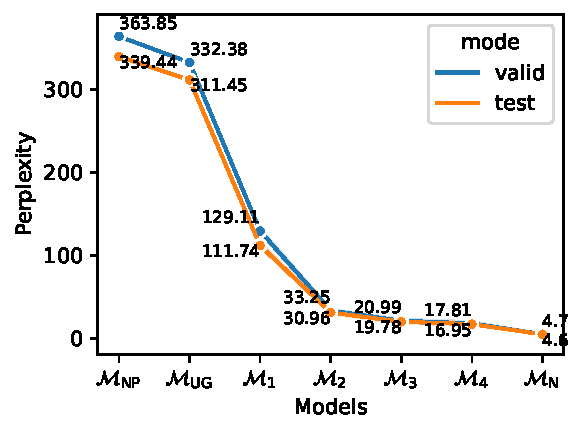
\includegraphics{figs/mlm/perplexity.pdf}}
    \caption{Perplexity of various models on Wiki 103 valid and test sets.}
    \label{fig:mlm_perplexity}
\end{figure}


\subsection{Fine-tuning tasks}

We evaluate downstream performance using the General Language Understanding and Evaluation (GLUE) benchmark, the Paraphrase Adversaries from Word Scrambling (PAWS) dataset, and various parametric and non-parametric tasks (see \autoref{sec:mlm_probing_results}).

\xhdr{GLUE} %We use the GLUE \cite{wang2018glue} benchmark tasks to inspect the reliance of word order learning during pre-training. This
The GLUE \citep{wang-etal-2018-glue} benchmark is a collection of 9 datasets for evaluating natural language understanding systems, of which we use Corpus of Linguistic Acceptability \cite[CoLA,][]{cola_warstadt2019neural}, Stanford Sentiment Treebank \cite[SST,][]{sst2_socher2013recursive}, Microsoft Research Paragraph Corpus \cite[MRPC,][]{mrpc_dolan2005automatically}, Quora Question Pairs (QQP)\footnote{\href{http://data.quora.com/First-Quora-Dataset-Release-Question-Pairs}{http://data.quora.com/First-Quora-Dataset-Release-Question-Pairs}}, Multi-Genre NLI \cite[MNLI,][]{williams-etal-2018-broad}, Question NLI \cite[QNLI,][]{rajpurkar-etal-2016-squad, qnli_2_demszky2018transforming}, Recognizing Textual Entailment \cite[RTE,][]{Dagan2005:RTE, rte2_haim2006second, rte3_giampiccolo2007third, rte5_bentivogli2009fifth}.
\citet{pham-etal-2020-out} show the word order insensitivity of several GLUE tasks (QQP, SST-2), evaluated on public regularly pre-trained checkpoints.

\xhdr{PAWS} The PAWS task \citep{zhang-etal-2019-paws} consists of predicting whether a given pair of sentences are paraphrases. This dataset contains both paraphrase and non-paraphrase pairs with high lexical overlap, which are generated by controlled word swapping and back translation. Since even a small word swap and perturbation can drastically modify the meaning of the sentence, we hypothesize the randomized pre-trained models will struggle to attain a high performance on PAWS.

\xhdr{Fine-tuning details} We use the same fine-tuning methodology used by \citet{liu-et-al-2019-roberta}, where we run hyperparameter search over the learning rates $\{1 \times 10^{-5}, 2 \times 10^{-5}, 3 \times 10^{-5}\}$ and batch sizes $\{16, 32\}$ for each model.
For the best hyperparam configurations of each model, we fine-tune with 5 different seeds and report the mean and standard deviation for each setting. % (\autoref{table:glue_mean}).
\NP\ is fine-tuned without positional embeddings, matching the way it was pre-trained.

\section{Results}
\label{sec:mlm_results}

\subsection{Downstream task results}
\label{sec:mlm_downstream_results}


In this section, we present the downstream task performance of the models defined in \autoref{sec:mlm_experimental_setup}. For evaluation, we report Matthews correlation for CoLA and accuracy for all other tasks.

\subsubsection{Word order permuted pre-training}
\label{sec:mlm_glue_results}

\begin{table*}[t]
  \centering
  \resizebox{\linewidth}{!}{%
\begin{tabular}{lllllllll}
\toprule
Model & QNLI & RTE & QQP & SST-2 & MRPC & PAWS & MNLI-m/mm & CoLA \\ \midrule
\OR & 92.45 +/- 0.2 & 73.62 +/- 3.1 & 91.25 +/- 0.1 & 93.75 +/- 0.4 & 89.09 +/- 0.9 & 94.49 +/- 0.2 & 86.08 +/- 0.2 / 85.4 +/- 0.2 & 52.45 +/- 21 \\ \midrule
\RIV & 91.65 +/- 0.1 & 70.94 +/- 1.2 & 91.39 +/- 0.1 & 92.46 +/- 0.3 & 86.90 +/- 0.3 & 94.26 +/- 0.2 & 83.79 +/- 0.2 / 83.94 +/- 0.3 & 35.25 +/- 32 \\ 
\RIII & 91.56 +/- 0.4 & 69.75 +/- 2.8 & 91.22 +/- 0.1 & 91.97 +/- 0.5 & 86.22 +/- 0.8 & 94.03 +/- 0.1 & 83.83 +/- 0.2 / 83.71 +/- 0.1 & 40.78 +/- 23 \\
\RII & 90.51 +/- 0.1 & 70.00 +/- 2.5 & 91.33 +/- 0.0 & 91.78 +/- 0.3 & 85.90 +/- 1.2 & 93.53 +/- 0.3 & 83.45 +/- 0.3 / 83.54 +/- 0.3 & 50.83 +/- 5.8 \\
\RI & 89.05 +/- 0.2 & 68.48 +/- 2.5 & 91.01 +/- 0.0 & 90.41 +/- 0.4 & 86.06 +/- 0.8 & 89.69 +/- 0.6 & 82.64 +/- 0.1 / 82.67 +/- 0.2 & 31.08 +/- 10 \\
\midrule
\NP & 77.59 +/- 0.3 & 54.78 +/- 2.2 & 87.78 +/- 0.4 & 83.21 +/- 0.6 & 72.78 +/- 1.6 & 57.22 +/- 1.2 & 63.35 +/- 0.4 / 63.63 +/- 0.2 & 2.37 +/- 3.2 \\
%\RU & 77.69 +/- 0.4 & 53.84 +/- 0.6 & 85.92 +/- 0.1 & 84.00 +/- 0.6 & 71.35 +/- 0.8 & 58.43 +/- 0.3 & 72.10 +/- 0.4 / 72.58 +/- 0.4 & 8.89 +/- 1.40 \\
\RC & 66.94 +/- 9.2 & 53.70 +/- 1.0 & 85.57 +/- 0.1 & 83.17 +/- 1.5 & 70.57 +/- 0.7 & 58.59 +/- 0.3 & 71.93 +/- 0.2 / 71.33 +/- 0.5 & 0.92 +/- 2.1 \\
\RT & 62.17 +/- 0.4 & 52.97 +/- 0.2 & 81.53 +/- 0.2 & 82.0 +/- 0.7 & 70.32 +/- 1.5 & 56.62 +/- 0.0 & 65.70 +/- 0.2 / 65.75 +/- 0.3 & 8.06 +/- 1.6 \\
 \bottomrule
\end{tabular}}
\caption{GLUE and PAWS-Wiki dev set results on different RoBERTa (base) models trained on variants of the BookWiki corpus (with mean and std). The top row is the original model, the middle half contains our primary models under investigation, and the bottom half contains the baselines.}
\label{table:glue_mean}
\end{table*}


\begin{figure*}[ht]
    \centering
    \resizebox{\textwidth}{!}{
        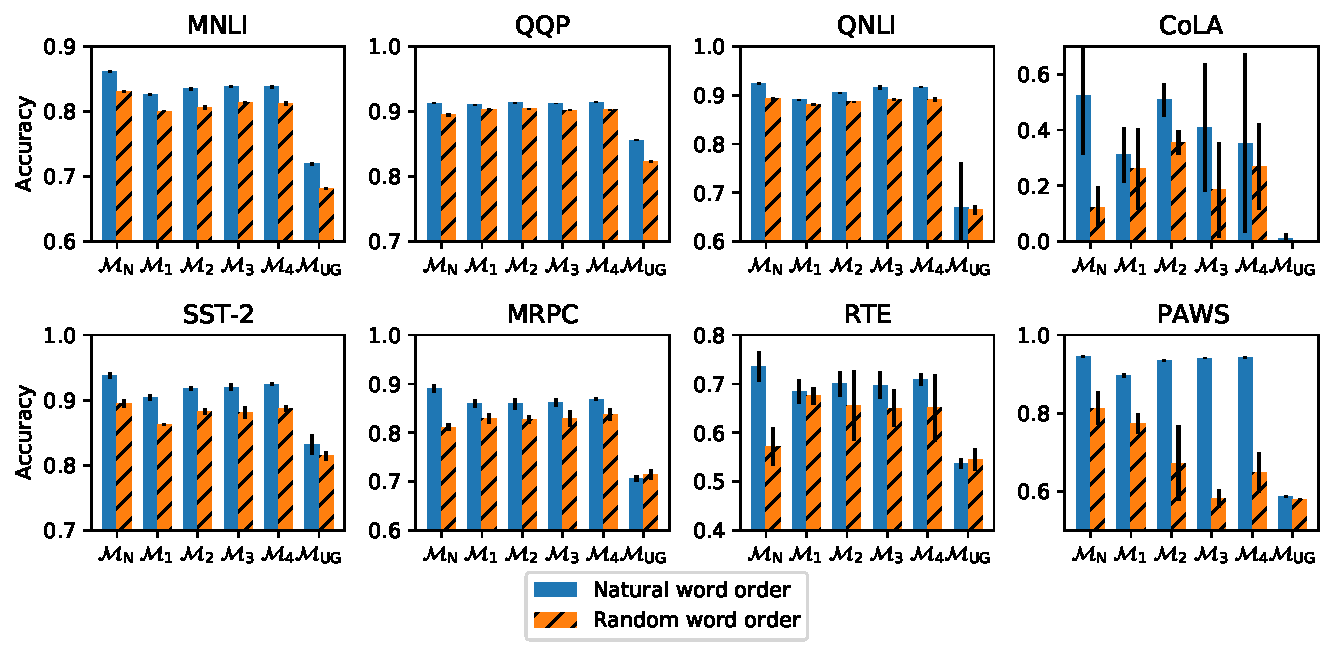
\includegraphics{figs/mlm/finetune_rand.pdf}}
    \caption{GLUE \& PAWS task dev performance when finetuned on naturally (blue) and randomly ordered (orange) text, respectively, using pre-trained RoBERTa (base) models trained on different versions of BookWiki corpus.}
    \label{fig:mlm_word_order_glue}
\end{figure*}

In our first set of experiments, we finetune the pre-trained models
%\OR, \RI, \RII, \RIII, \RIV\ and \RC\
on the GLUE and PAWS tasks.
We report the results in \autoref{table:glue_mean}.\footnote{The \OR\ results are not directly comparable with that of publicly released \texttt{roberta-base} model by \citet{liu-et-al-2019-roberta}, as that uses the significantly larger 160GB corpus, and is trained for 500K updates. For computational reasons, we restrict our experiments to the 16GB BookWiki corpus and 100K updates, mirroring the RoBERTa ablations.}
First, we observe that the model without access to distributional or word order information, \RC\ (unigram) performs much worse than \OR\ overall:
\RC\ is $18$ points worse than \OR\ on average across the accuracy-based tasks in \autoref{table:glue_mean} and has essentially no correlation with human judgments on CoLA. \RC\, \NP\ and \RT\ perform comparably on most of the tasks, while achieving surprisingly high scores in QQP and SST-2. However, all three models perform significantly worse on GLUE and PAWS, compared to \OR\ (\autoref{table:glue_mean}, bottom half).
\RC\ reaches up to $71.9$ on MNLI - possibly due to the fact that \RC\ has access to (bags of) words and some phrases (from NER) is beneficial for MNLI. For the majority of tasks, the difference between \NP\ and \RT\ is small - a pure bag of words model performs comparably to a randomly initialized model.

Next, we observe a significant improvement on all tasks when we give models access to sentence-level distributional information during pre-training.
\RI, the model pre-trained on completely shuffled sentences, is on average only $3.3$ points lower than \OR\ on the accuracy-based tasks,
and within $0.3$ points of \OR\ on QQP.
Even on PAWS, which was designed to require knowledge of word order, \RI\ is within $5$ points of \OR.
Randomizing $n$-grams instead of words during pre-training results in a (mostly) smooth increase on these tasks: \RIV, the model pre-trained on shuffled $4$-grams, trails \OR\ by only $1.3$ points on average, and even comes within $0.2$ points of \OR\ on PAWS.
%Compared to \citet{pham-etal-2020-out} results, our observations on the gap between \OR and shuffled pre-train models to be much closer than their observations.
We observe a somewhat different pattern on CoLA, where \RII\ does almost as well as \OR\ and outperforms \RIII\ and \RIV, though we also observe very high variance across random seeds for this task.
Crucially, we observe that \RI\ outperforms \NP\ by a large margin. This shows that positional embeddings are critical for learning, even when the word orders themselves are not natural. Recall, \NP\ is fed natural sentences as \OR\, while not having the ability to learn positional embeddings. To further quantify the effect of positional embeddings, we also investigated the effect of shuffling the entire context window, to keep the co-occurrence information same as \NP\ in \autoref{sec:mlm_ablations}. We observed this model to be worse than \RI\, but significantly better than \NP\, to support the claim about the importance of positional embeddings while training.

Overall, these results confirm our hypothesis that RoBERTa's strong performance on downstream tasks can be explained for a large part by the distributional prior.

\subsubsection{Word order permuted fine-tuning}

There are two possible explanations for the results in \autoref{sec:mlm_glue_results}: either the tasks do not need word order information to be solved, or any necessary word order information can be acquired during fine-tuning.
To examine this question, we permute the word order during fine-tuning as well.
%A natural question arises following the results from the previous section: does pre-training capture most of the word order information, or does finetuning on the downstream task contribute more to a model's knowledge of word order? To disentangle the cause and effect, we use our set of models to finetune on a randomized version of the downstream tasks.
%TODO: Do this at the sentence level or be MUCH more explicit that this is NOT at the sentence level:
Concretely, for each task, we construct a unigram order-randomized version of each example in the fine-tuning training set using $\mathcal{F}_1$. We then fine-tune our pre-trained models on this shuffled data and evaluate task performance. For all experiments, we evaluate and perform early stopping on the original, natural word order dev set, in order to conduct a fair evaluation on the exact same optimization setup for all models.
%

Our results in \autoref{fig:mlm_word_order_glue} provide some evidence for both hypotheses.
%provide some evidence for both hypotheses, but primarily show that shuffled models \emph{are} learning to use word order-related information during fine-tuning.
On QQP and QNLI, accuracy decreases only slightly for models fine-tuned on shuffled data. %, suggesting that word order is not very important for these tasks.
Models can also achieve above $80\%$ accuracy on MNLI, SST-2, and MRPC when fine-tuned on shuffled data,
suggesting that purely lexical information is quite useful on its own.
% \footnote{
% This finding is compatible with the observation of \citet{gupta-etal-2021-bert} and \citet{sinha2020b} who train on a randomized training corpus for MRPC, QQP, SST-2 and MNLI.}

On the other hand, for all datasets besides QQP and QNLI, we see noticeable drops in accuracy when fine-tuning on shuffled data and testing on normal order, both for \OR\ and for shuffled models \RI\ through \RIV.
This suggests both that word order information is useful for these tasks, and that shuffled models must be learning to use word order information during fine-tuning.\footnote{We perform additional experiments on how the model representations change during fine-tuning for shuffled training using Risannen Data Analysis in \autoref{sec:mlm_rda_analysis}.}
Having word order during fine-tuning is especially important for achieving high accuracy on CoLA, RTE (cf. \citealt{pham-etal-2020-out}), as well as PAWS,
suggesting that these tasks are the most word order reliant. Recent research \citep{yu-ettinger-2021-interplay} raised some questions about potential artefacts inflating performance on PAWS: their swapping-distance cue of appears consistent both with our finding of high PAWS performance for n-gram shuffled models in \autoref{table:glue_mean}, and with our PAWS results in \autoref{fig:mlm_word_order_glue}, which suggests that PAWS performance does in fact rely to some extent on natural word order  at the fine-tuning stage.

Finally, for CoLA, MRPC, and RTE, performance is higher after fine-tuning on shuffled data for \RI\ than \OR.
We hypothesize that \OR\ represents shuffled and non-shuffled sentences very differently, resulting in a domain mismatch problem when fine-tuning on shuffled data but evaluating on non-shuffled data.\footnote{We further study the domain mismatch problem by evaluating on shuffled data \textit{after} fine-tuning on the shuffled data for models in \autoref{sec:mlm_rand_eval}. We observe that models improves their scores on evaluation on shuffled data when the training data source is changed from natural to shuffled - highlighting domain match effect.} Since \RI\ never learns to be sensitive to word order during pre-training or fine-tuning, it does not suffer from that issue. Our results in this section also highlights the issues with these datasets, concurrent to the findings that many GLUE tasks does not need sophisticated linguistic knowledge to solve, as models typically tend to exploit the statistical artefacts and spurious correlations during fine-tuning (cf. \citealt{gururangan-etal-2018-annotation, poliak-etal-2018-hypothesis,tsuchiya-2018-performance,mccoy-etal-2019-right}). However, our results overwhelmingly support the fact that word order does not matter during pre-training, if the model has the opportunity to learn the necessary information about word order during fine-tuning.

\subsection{Probing results}
\label{sec:mlm_probing_results}

%Downstream tasks paint only a partial picture of the information contained in the pre-trained representation.
To investigate how much syntactic information is contained in the \acrshort{mlm} representations, we evaluate several probing tasks on our trained models. We consider two classes of probes: \textit{parametric} probes, which make use of learnable parameters, and \textit{non-parametric} probes, which directly examine the language model's predictions.

\subsubsection{Parametric Probing}
\label{sec:mlm_param_probing}

To probe our models for syntactic, semantic and other linguistic properties, we investigate dependency parsing using Pareto probing~\citep{pimentel-etal-2020-pareto} and the probing tasks from \cite{conneau-etal-2018-cram} in SentEval~\citep{conneau-kiela-2018-senteval}.

\citet{pimentel-etal-2020-pareto} proposed a framework based on Pareto optimality to probe for syntactic information in contextual representations. They suggest that an optimal probe should balance optimal performance on the probing task with the complexity of the probe. Following their setup, we use the ``difficult'' probe: dependency parsing (DEP). We also investigate the ``easy'' probes, dependency arc labeling (DAL) and POS tag prediction (POS), results are reported \autoref{sec:mlm_pareto_probes}.
We probe with Linear and MLP probes, and inspect the task accuracy in terms of Unlabeled Attachment Score (UAS).
The dependency parsing probe used in \citet{pimentel-etal-2020-pareto} builds on the Biaffine Dependency Parser~\citep{dozat2016deep}, but with simple MLPs on top of the Transformer representations.%
%the complexity of the probe reduced by using only simple MLPs on top of the Transformer representations.
%removing the LSTM layer to restrict access to context. This probe consists of two identical MLPs - one to process the heads of the dependencies, and another to process the tails. The final biaffine transformation is simply a learned mapping function among output of the MLPs which is normalized to obtain the probabilities.
\footnote{We experimented with a much stronger, state-of-the-art Second order Tree CRF Neural Dependency Parser \cite{zhang-etal-2020-efficient}, but did not observe any difference in UAS with different pre-trained models (see \autoref{sec:mlm_sota_dep})}

\xhdr{Training setup} Similar to the setup by \citet{pimentel-etal-2020-pareto}, we run 50 random hyperparameter searches on both MLP and Linear probes by uniformly sampling from the number of layers (0-5), dropout (0-0.5), log-uniform hidden size $[2^{5}, 2^{10}]$. We triple this experiment size by evaluating on three pre-trained models of different seeds for each model configuration.
We consider \citeauthor{pimentel-etal-2020-pareto}'s English dataset, derived from Universal Dependencies EWT (UD EWT) \citep{bies2012english, silveira2014gold} which contains 12,543 training sentences.
%Since \citet{pimentel-etal-2020-pareto} explored multi-lingual corpora, they only experimented with a single English dataset, derived from Universal Dependencies EWT (UD EWT) \cite{bies2012english, silveira2014gold} containing 12,543 training sentences.
Additionally, we experiment on the Penn Treebank dataset (PTB), which contains 39,832 training sentences.\footnote{PTB data \citep{kitaev-etal-2019-multilingual} is used from \href{https://github.com/nikitakit/self-attentive-parser/tree/master/data}{github.com/nikitakit/self-attentive-parser/tree/master/data}.}
%Since \citet{pimentel-etal-2020-pareto} explored multi-lingual corpora, they only experimented with a single English dataset, derived from Universal Dependencies EWT (UD EWT) \cite{bies2012english, silveira2014gold} containing 12,543 training sentences. Additionally, we experiment on the Penn Treebank dataset (PTB), which contains 39,832 training sentences.\footnote{PTB data \citep{kitaev-etal-2019-multilingual} is used from \href{https://github.com/nikitakit/self-attentive-parser/tree/master/data}{github.com/nikitakit/self-attentive-parser/tree/master/data}.}
We report the mean test accuracy over three seeds for the best dev set accuracy for each task.\footnote{\citet{pimentel-etal-2020-pareto} propose computing the \textit{Pareto Hypervolume} over all hyperparameters in each task. We did not observe a significant difference in the hypervolumes for the models, as reported in \autoref{sec:mlm_pareto_probes}.}

\begin{table}[]
\centering
\resizebox{0.6\linewidth}{!}{%
\begin{tabular}{l|rl|rl}
\toprule
Model & \multicolumn{2}{c|}{UD EWT} & \multicolumn{2}{c}{PTB} \\ \hline
 & MLP & Linear & MLP & Linear \\ \cline{2-5} 
\OR & 80.41 +/- 0.85 & 66.26 +/- 1.59 & 86.99 +/- 1.49 & 66.47 +/- 2.77 \\\midrule
\RIV & 78.04 +/- 2.06 & 65.61 +/- 1.99 & 85.62 +/- 1.09 & 66.49 +/- 2.02 \\
\RIII & 77.80 +/- 3.09 & 64.89 +/- 2.63 & 85.89 +/- 1.01 & 66.11 +/- 1.68 \\
\RII & 78.22 +/- 0.88 & 64.96 +/- 2.32 & 84.72 +/- 0.55 & 64.69 +/- 2.50 \\
\RI & 69.26 +/- 6.00 & 56.24 +/- 5.05 & 79.43 +/- 0.96 & 57.20 +/- 2.76 \\\midrule
\RC & 74.15 +/- 0.93 & 65.69 +/- 7.35 & 80.07 +/- 0.79 & 57.28 +/- 1.42 \\
\bottomrule
\end{tabular}%
}
\caption{Unlabeled Attachment Score (UAS) (mean and std) on the dependency parsing task (DEP) on two datasets, UD EWT and PTB, using the Pareto Probing framework \citep{pimentel-etal-2020-pareto}.}
\label{tab:pareto_dependency}
\end{table}


\begin{table*}[ht]
  \centering
  \resizebox{\linewidth}{!}{%
\begin{tabular}{lrrrrrrrrrr}
\toprule
                      \textbf{Model} &          \textbf{Length} &     \textbf{WordContent} &           \textbf{TreeDepth} & \textbf{TopConstituents} &     \textbf{BigramShift} &           \textbf{Tense} & \textbf{SubjNumber} &  \textbf{ObjNumber} &       \textbf{OddManOut} & \textbf{CoordInversion} \\
                      & (Surface) & (Surface) & (Syntactic) & (Syntactic)  & (Syntactic) & (Semantic)  & (Semantic) & (Semantic) & (Semantic) & (Semantic) \\
\midrule
\OR &  78.92 +/- 1.91 &  31.83 +/- 1.75 &  35.97 +/- 1.38 &  \textbf{78.26} +/- 4.08 &  \textbf{81.82} +/- 0.55 &  87.83 +/- 0.51 &  85.05 +/- 1.23 &  75.94 +/- 0.68 &   58.40 +/- 0.33 &        \textbf{70.87} +/- 2.46 \\\midrule
\RIV &  92.88 +/- 0.15 &  57.78 +/- 0.36 &  40.05 +/- 0.29 &   72.50 +/- 0.51 &  76.12 +/- 0.29 &  88.32 +/- 0.13 &  \textbf{85.65} +/- 0.13 &  82.95 +/- 0.05 &   \textbf{58.89} +/- 0.30 &        61.31 +/- 0.19 \\
\RIII &  91.52 +/- 0.16 &  48.81 +/- 0.26 &  38.63 +/- 0.61 &  70.29 +/- 0.31 &  77.36 +/- 0.12 &  86.74 +/- 0.12 &  83.83 +/- 0.38 &  80.99 +/- 0.26 &  57.01 +/- 0.21 &         60.00 +/- 0.26 \\
\RII &  \textbf{93.54} +/- 0.29 &  62.52 +/- 0.21 &   \textbf{41.40} +/- 0.32 &  74.31 +/- 0.29 &  75.44 +/- 0.14 &  \textbf{87.91} +/- 0.35 &  84.88 +/- 0.11 &  83.98 +/- 0.14 &   57.60 +/- 0.36 &        59.46 +/- 0.37 \\
\RI &  88.33 +/- 0.14 &  \textbf{64.03} +/- 0.34 &   40.24 +/- 0.20 &  70.94 +/- 0.38 &   58.37 +/- 0.40 &  87.88 +/- 0.08 &  83.49 +/- 0.12 &  \textbf{83.44} +/- 0.06 &  56.51 +/- 0.26 &         56.98 +/- 0.50 \\
\midrule
\RC &  86.69 +/- 0.33 &   36.60 +/- 0.33 &  32.53 +/- 0.76 &   61.54 +/- 0.60 &  57.42 +/- 0.04 &  68.45 +/- 0.23 &  71.25 +/- 0.12 &  66.63 +/- 0.21 &   50.06 +/- 0.40 &        56.26 +/- 0.17 \\ 
%\hline
%\texttt{RB} &   75.86 &    27.4 &   34.02  &   71.85  &   88.43 &   88.32  &   84.01 &   81.83 &   66.41  &         70.68 \\
\bottomrule
\end{tabular}}
\caption{SentEval Probing \citep{conneau-etal-2018-cram, conneau-kiela-2018-senteval} results (with mean and std) on different model variants.}
%Results on the publicly available Roberta (base) (\texttt{RB}) from \citet{liu2019b} provided for comparison.
\label{table:senteval}
\end{table*}


\xhdr{Results} We observe that
the UAS scores follow a similar linear trend as the fine-tuning results in that \RI $\approx$ \RC < \RII < \RIII < \RIV < \OR\ (\autoref{tab:pareto_dependency}).
Surprisingly, \RC\ probing scores seem to be somewhat better than \RI\ (though with large overlap in their standard deviations), even though \RC\ cannot learn information related to either word order or co-occurrence patterns.
The performance gap appears to be task- and probe specific.
%The gap in UAS between \RI and \OR\ for UD EWT is higher than that of the counterpart in PTB ($11.15$ vs. $7.56$). This trend is also mildly reflected in the case of the Linear probe ($10.02$ vs. $9.27$ UD EWT).
We observe a low performance gap in several scenarios, the lowest being between \OR\ vs. \RIII/\RIV, for PTB using the both MLP and Linear probes.
%These results are an indicator of possible deficiencies in the method of testing representations for syntactic information.

\subsubsection{SentEval Probes}

We also investigate the suite of 10 probing tasks~\citep{conneau-etal-2018-cram} available in the SentEval toolkit~\citep{conneau-kiela-2018-senteval}. This suite contains a range of semantic, syntactic and surface level tasks. \citet{jawahar2019a} utilize this set of probing tasks to arrive at the conclusion that %that BERT-based models naturally learn syntax -
``\textit{BERT embeds a rich hierarchy of linguistic signals: surface information at the bottom, syntactic information in the middle, semantic information at the top}''. We re-examine this hypothesis by using the same probing method and comparing against models trained with random word order.

\xhdr{Training setup} We run the probes on the final layer of each of our pre-trained models for three seeds, while keeping the encoder frozen. % It is important to note that SentEval probe evaluates on frozen encoder representations.
SentEval %obtains the sentence representations from the model under investigation, and then
trains %linear and two-layer MLP
probes on top of fixed representations individually for each task. We follow the recommended setup and run grid search over the following hyperparams: number of hidden layer dimensions ($[0,50,100,200]$), dropout ($[0, 0.1, 0.2]$), 4 epochs, 64 batch size.
%For all hyperparameters,
We select the best performance based on the dev set, and report the test set accuracy.

\xhdr{Results} We provide the results in \autoref{table:senteval}. The \OR\ pre-trained model scores better than the unnatural word order models for only one out of five semantic tasks and in none of the lexical tasks. However, \OR\ does score higher for two out of three syntactic tasks. Even for these two syntactic tasks, the gap among \RC\ and \OR\ is much higher than \RI\ and \OR. These results show that while natural word order is useful for at least some probing tasks, the distributional prior of randomized models alone is enough to achieve a reasonably high accuracy on syntax sensitive probing.

\subsubsection{Non-Parametric Probing}
\label{sec:non_param_probe}


How to probe effectively with parametric probes is a matter of much recent debate~\citep{hall-maudslay-etal-2020-tale, belinkov2021probing}. From our results so far, it is unclear whether parametric probing meaningfully distinguishes models trained with corrupted word order from those trained with normal orders. Thus, we also investigate non-parametric probes~\citep{linzen-etal-2016-assessing,marvin-linzen-2018-targeted,gulordava-etal-2018-colorless} using the formulation of \citet{goldberg2019assessing} and \citet{wolf2019}.% Since these probes do not contain any learnable parameters, they are called ``non-parametric''.

We consider a set of non-parametric probes that use a range of sentences varying in their linguistic properties. For each, the objective is for a pre-trained model to provide higher probability to a grammatically correct word than to an incorrect one.
Since both the correct and incorrect options occupy the same sentential position, we call them ``focus words''. \citet{linzen-etal-2016-assessing} use sentences from Wikipedia containing present-tense verbs, and compare the probability assigned by the encoder to plural vs. singular forms of the verb; they focus on sentences containing at least one noun between the verb and its subject, known as ``agreement attractors.'' \citet{gulordava-etal-2018-colorless} instead replace focus words with random substitutes from the same part-of-speech and inflection. Finally, \citet{marvin-linzen-2018-targeted} construct minimal pairs of grammatical and ungrammatical sentences, and compare the model's probability for the words that differ.

\xhdr{Setup} In our experiments, we mask the focus words in the stimuli and compute the probability of the correct and incorrect token respectively.
To handle Byte-Pair Encoding (BPE), we use the WordPiece \citep{wu2016googles} tokens prepended with a space. %, as used in RoBERTa to compute the probability of a correct focus word and an incorrect focus word. D: this says the same thing as the first clause of this sentence, removed it
We observe that the \citet{linzen-etal-2016-assessing} and \citet{gulordava-etal-2018-colorless} datasets are skewed towards singular focus words, which could disproportionately help weaker models that just happen to assign more probability mass to singular focus words. To counter this, we balance these datasets to have an equal number of singular and plural focus words by upsampling, and report the aggregated and balanced results in \autoref{tab:non_param_comb} (see \autoref{sec:mlm_non_par_probes} for more detailed results). We verify our experiments by using three pre-trained models with different seeds for each model configuration.


\xhdr{Results}
We observe for the \citet{linzen-etal-2016-assessing} and \citet{marvin-linzen-2018-targeted} datasets that the gap between the \OR\ and randomization models is relatively large.
The \citet{gulordava-etal-2018-colorless} dataset shows a smaller gap between \OR\ and the randomization models. While some randomization models (e.g., \RII, \RIII, and \RIV) performed quite similarly to \OR\ according to the parametric probes, they all are markedly worse than \OR\ according to the non-parametric ones. This suggests that non-parametric probes identify certain syntax-related modeling failures
that parametric ones do not.

% \begin{table}
%   \centering
%   \resizebox{\linewidth}{!}{%
% \begin{tabular}{llll}
% Model & \citet{linzen-etal-2016-assessing} & \citet{gulordava2018} & \citet{marvin2018a} \\
% \midrule
% \OR & 91.17 (2.61) [23.26] & 68.66 (11.56) [1.97] & 88.21 (6.71) [14.53]\\
% \RC & 65.36 (7.06) [1e-4] & 60.88 (24.26) [1e-4] & 50.13 (0.24) [1e-4]\\
% \RI & 58.96 (1.82) [0.07] & 68.1 (14.42) [0.03] & 70.45 (11.42) [0.49]\\
% \RII & 61.27 (3.07) [1.01] & 60.2 (7.64) [1e-4] & 74.08 (14.33) [1.06]\\
% \RIII & 64.6 (2.71)  [2.25] & 66.1 (5.99) [0.24] & 73.78 (15.64) [1.62]\\
% \RIV & 66.93 (3.2)  [3.22] & 69.47 (4.99) [0.46] & 70.8 (12.6) [3.84]\\
% \bottomrule
% \end{tabular}}
% \caption{Mean accuracy of non-parametric probing on different stimuli datasets. Values in paranthesis reflects the standard deviation over sub-tasks. Values in square brackets indicate the mean probability difference.}
% \label{tab:non_param_comb}
% \end{table}

\begin{table}
  \centering
  \resizebox{\linewidth}{!}{%
\begin{tabular}{lrrr}
\toprule
Model & \citet{linzen-etal-2016-assessing} $^*$ & \citet{gulordava2018} $^*$ & \citet{marvin-linzen-2018-targeted} \\
\midrule
\OR & 91.17 +/- 2.6 & 68.66 +/- 11.6 & 88.05 +/- 6.5 \\
\RIV & 66.93 +/- 3.2 & 69.47 +/- 4.9  & 70.66 +/- 12.5 \\
\RIII & 64.60 +/- 2.7 & 66.10 +/- 5.9  & 73.82 +/- 15.7 \\
\RII & 61.27 +/- 3.1 & 60.20 +/- 7.6  & 73.95 +/- 14.3 \\
\RI & 58.96 +/- 1.8 & 68.10 +/- 14.4 & 70.69 +/- 11.6 \\
\RC & 65.36 +/- 7.1 & 60.88 +/- 24.3 & 50.10 +/- 0.2 \\
\bottomrule
\end{tabular}}
\caption{Mean (and std) non-parametric probing accuracy on different datasets. $^*$ indicates rebalanced datasets, see \autoref{sec:mlm_non_par_probes} for more details.}
\label{tab:non_param_comb}
\end{table}


\section{Analysis}
\label{sec:mlm_analysis}


\subsection{Word-order pre-training ablations}
\label{sec:mlm_ablations}

\begin{table*}[t]
  \centering
  \resizebox{\linewidth}{!}{%
\begin{tabular}{lllllllll}
\toprule
Model & QNLI & RTE & QQP & SST-2 & MRPC & PAWS & MNLI-m/mm & CoLA \\ \midrule
\OR & 92.45 +/- 0.2 & 73.62 +/- 3.1 & 91.25 +/- 0.1 & 93.75 +/- 0.4 & 89.09 +/- 0.9 & 94.49 +/- 0.2 & 86.08 +/- 0.2 / 85.4 +/- 0.2 & 52.45 +/- 21.2 \\ \midrule
\RIV & 91.65 +/- 0.1 & 70.94 +/- 1.2 & 91.39 +/- 0.1 & 92.46 +/- 0.3 & 86.90 +/- 0.3 & 94.26 +/- 0.2 & 83.79 +/- 0.2 / 83.94 +/- 0.3 & 35.25 +/- 32.2 \\ 
\RIII & 91.56 +/- 0.4 & 69.75 +/- 2.8 & 91.22 +/- 0.1 & 91.97 +/- 0.5 & 86.22 +/- 0.8 & 94.03 +/- 0.1 & 83.83 +/- 0.2 / 83.71 +/- 0.1 & 40.78 +/- 23.0 \\
\RII & 90.51 +/- 0.1 & 70.00 +/- 2.5 & 91.33 +/- 0.0 & 91.78 +/- 0.3 & 85.90 +/- 1.2 & 93.53 +/- 0.3 & 83.45 +/- 0.3 / 83.54 +/- 0.3 & 50.83 +/- 5.80 \\
\RI & 89.05 +/- 0.2 & 68.48 +/- 2.5 & 91.01 +/- 0.0 & 90.41 +/- 0.4 & 86.06 +/- 0.8 & 89.69 +/- 0.6 & 82.64 +/- 0.1 / 82.67 +/- 0.2 & 31.08 +/- 10.0 \\
\midrule
\RV & 84.97 +/- 0.3 & 56.09 +/- 0.6 & 90.15 +/- 0.1 & 86.11 +/- 0.7 & 79.41 +/- 0.6 & 77.3 +/- 12.63 & 77.58 +/- 0.3 / 77.89 +/- 0.4 & 12.54 +/- 5.57 \\
\NP & 77.59 +/- 0.3 & 54.78 +/- 2.2 & 87.78 +/- 0.4 & 83.21 +/- 0.6 & 72.78 +/- 1.6 & 57.22 +/- 1.2 & 63.35 +/- 0.4 / 63.63 +/- 0.2 & 2.37 +/- 3.20 \\
\RU & 77.69 +/- 0.4 & 53.84 +/- 0.6 & 85.92 +/- 0.1 & 84.00 +/- 0.6 & 71.35 +/- 0.8 & 58.43 +/- 0.3 & 72.10 +/- 0.4 / 72.58 +/- 0.4 & 8.89 +/- 1.40 \\
\RC & 66.94 +/- 9.2 & 53.70 +/- 1.0 & 85.57 +/- 0.1 & 83.17 +/- 1.5 & 70.57 +/- 0.7 & 58.59 +/- 0.3 & 71.93 +/- 0.2 / 71.33 +/- 0.5 & 0.92 +/- 2.10 \\
\RT & 62.17 +/- 0.4 & 52.97 +/- 0.2 & 81.53 +/- 0.2 & 82.0 +/- 0.7 & 70.32 +/- 1.5 & 56.62 +/- 0.0 & 65.70 +/- 0.2 / 65.75 +/- 0.3 & 8.06 +/- 1.60 \\

 \bottomrule
\end{tabular}}
\caption{GLUE and PAWS-Wiki dev set results on different ablations of the RoBERTa (base) models, trained on variants of the BookWiki corpus (with mean and std dev). The top row is the original model, the middle half contains the sentence randomization models, and the bottom half contains the ablations.}
\label{table:glue_ablations}
\end{table*}

\begin{figure}[t]
    \centering
    \resizebox{0.7\textwidth}{!}{
        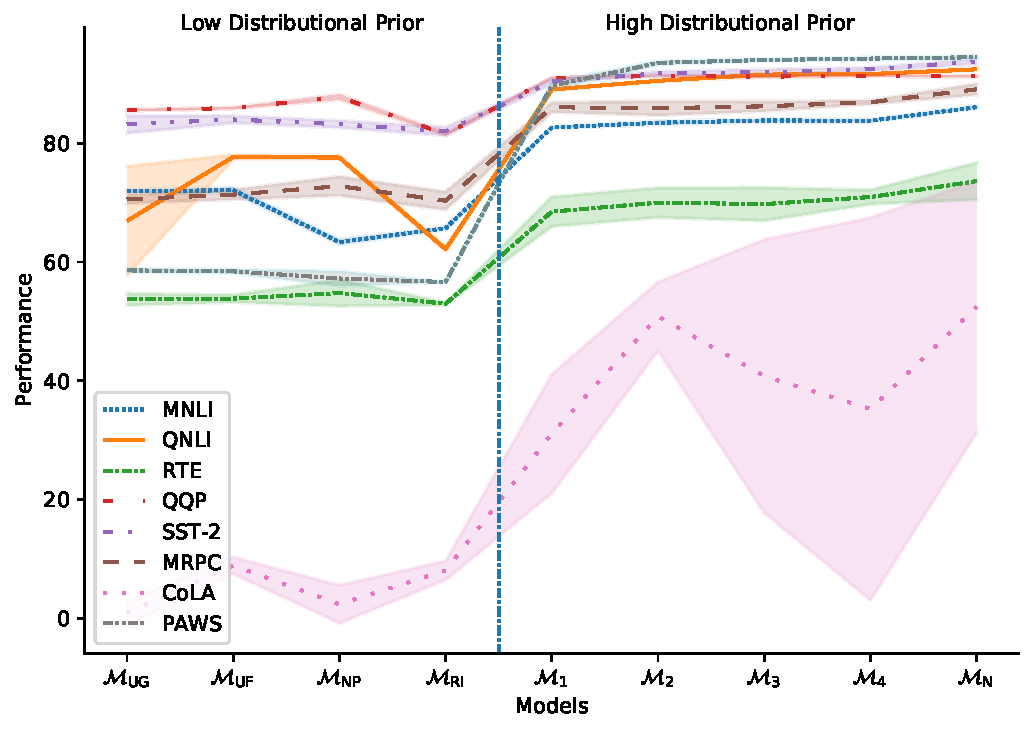
\includegraphics{figs/mlm/main_result_plot.pdf}}
    \caption{GLUE results on various model ablations using BookWiki corpus.}
    \label{fig:mlm_all_glue_plot}
\end{figure}

We also train further model ablations with low to high distributional priors. Following the construction of the corpus bootstrap resample, we train a model where words are drawn uniformly from BookWiki corpus, thus destroying the natural frequency distribution (\RU). We further study an ablation for a high distributional prior, \RV, where we shuffle words (unigram) in a buffer created with joining multiple sentences such that maximum token length of the buffer is 512. This ablation---which is similar to the paragraph word shuffle condition in \cite{gauthier-levy-2019-linking}---will allow us to study the effect of unigram shuffling in a window larger than the one for \RI. Buffer size is chosen to be 512 because BERT/RoBERTa is typically trained with that maximum sequence length.

We observe dev set results on the GLUE benchmark of these ablations, along with baselines \RC, \RT\ and \NP\ and random shuffles in \autoref{table:glue_ablations} and \autoref{fig:mlm_all_glue_plot}. We observe that \RV\ exhibits worse overall scores than \RI, however it is still significantly better than \NP\ or \RC\ baselines. We observe that destroying the natural frequency distribution of words (\RU) yields comparable or slightly better results compared to random corpus model \RC. This result shows that merely replicating the natural distribution of words without any context is not useful for the model to learn. These results indicate that at least some form of distributional prior is required for \acrshort{mlm}-based models to learn a good downstream representation.

\begin{table}[t]
  \centering
  \resizebox{0.8\linewidth}{!}{%
   \begin{tabular}{lrrrrrrrr}
\toprule
         Model &   RTE &  MRPC &  SST-2 &  CoLA &   QQP &  QNLI &  MNLI &  PAWS \\
\midrule
\RI & 68.48 & 85.97 &  90.41 & 31.07 & 91.01 & 89.05 & 82.64 & 89.69 \\
\RI$^*$ & 68.41 & 85.75 &  90.17 & 50.14 & 91.02 & 89.50 & 82.92 & 91.99 \\
\bottomrule
   \end{tabular}}
   \caption{Reconstruction experiments on shuffled word order sentences by fixing the same seed for every sentence (\RI) and having different seed for different shards of the corpus (\RI$^{*}$). We observe minimal difference in the downstream GLUE and PAWS scores.}
   \label{table:glue_recon}
\end{table}


One might argue that the superior results displayed by the unnatural models is due to the ability of RoBERTa to ``reconstruct'' the natural word order from shuffled sentences. The data generation algorithm, $\mathcal{F}_{i}$ requires a seed $t$ for every sentence. In our experiments, we had set the same seed for every sentence in the corpus to ensure reproducibility. However, it could be problematic if the sentences of the same length are permuted with the same seed, which could be easier for the model to ``reconstruct'' the natural word order to learn the necessary syntax. We tested this hypothesis by constructing a new corpus with different seeds for every sentence in every shard in the corpus (1/5th of BookWiki corpus is typically referred to as a \textit{shard} for computational purposes), to build the model \RI$^{*}$. We observe that there is minimal difference in the raw numbers among \RI\ and \RI$^{*}$ for most of the tasks (\autoref{table:glue_recon}) (with the exception of CoLA which performs similar to \RII\, possibly due to a difference in initialization). This result consequently proves that even with same seed, it is difficult for the model to just reconstruct the unnatural sentences during pre-training.

\subsection{Measuring Relative difference}
\label{sec:mlm_rd}

In this section, we further measure the difference in downstream task performance reported in \autoref{sec:mlm_glue_results} using as a metric the \textit{relative difference}. Let us denote the downstream task performance as $\mathcal{A}(\mathcal{T} | D)$, where $\mathcal{T}$ is the task and $D$ is the pre-trained model. We primarily aim to evaluate the relative performance gap, i.e. how much the performance differs between our natural and unnatural models. Thus, we define the \textit{Relative Difference} ($\Delta_{\{D\}}(\mathcal{T})$):

\begin{equation}
 \Delta_{\{D\}}(\mathcal{T}) =  \frac{\mathcal{A}(\mathcal{T} | OR) - \mathcal{A}(\mathcal{T} | D))}{\mathcal{A}(\mathcal{T} | OR) - \mathcal{A}(\mathcal{T} | \emptyset)},
\end{equation}

where $\mathcal{A}(\mathcal{T} | \emptyset)$ is the random performance on the task $\mathcal{T}$ ($0.33$ for MNLI, $0$ for CoLA, and $0.5$ for rest)
$\Delta_{\{D\}}(\mathcal{T}) \rightarrow 0$ when the performance of a pre-trained model reaches that of the pre-trained model trained with natural word order.

We observe the relative difference on the tasks in \autoref{tab:glue_delta}. CoLA has the largest $\Delta_{\{D\}}(\mathcal{T})$ among all tasks, suggesting the expected high word order reliance. $\Delta_{\{D\}}(\mathcal{T})$ is lowest for QQP. %, which falls on the opposite end of the spectrum.

\begin{table}[t]
  \centering
  \resizebox{0.8\linewidth}{!}{%
\begin{tabular}{lrrrrrrrr}
\toprule
Model &  QNLI &  RTE &  QQP &  SST-2 &  MRPC &  CoLA &  PAWS &  MNLI \\
\midrule
   \RI &    3.70 &   7.04 &   0.26 &     3.58 &    3.42 &   40.74 &    5.12 &  3.62 \\
   \RII &    2.11 &   4.95 &  -0.09 &     2.12 &    3.61 &    3.09 &    9.06 &  2.63 \\
   \RIII &    0.97 &   5.30 &   0.03 &     1.91 &    3.24 &   22.25 &    0.49 &  2.31 \\
   \RIV &    0.87 &   3.67 &  -0.15 &     1.39 &    2.47 &   32.79 &    0.25 &  2.19 \\\midrule
   \RC &   27.74 &  27.25 &   6.26 &    11.35 &   20.91 &   98.24 &   38.20 & 16.56 \\
   \NP &   16.16 &  25.77 &   3.83 &    11.30 &   18.42 &   95.48 &   39.66 & 26.10 \\
\bottomrule
\end{tabular}}
\caption{$ \Delta_{\{D_i\}}(\mathcal{T})$, scaled by a factor of 100 for GLUE and PAWS tasks.}
\label{tab:glue_delta}
\end{table}


\subsection{Fine-tuning with randomized data}
\label{sec:mlm_rand_eval}

\begin{table*}[t]
\centering
\resizebox{\linewidth}{!}{%
\begin{tabular}{llllllllll}
\toprule
name & fine-tune-train & fine-tune-eval &            MNLI &            QNLI &             RTE &             CoLA &            MRPC &           SST-2 &             PAWS \\
\midrule
 \OR &        natural &       natural &  86.08 +/- 0.15 &  92.45 +/- 0.24 &  73.62 +/- 3.09 &  52.44 +/- 21.22 &  89.09 +/- 0.88 &  93.75 +/- 0.44 &   94.49 +/- 0.18 \\
  &        natural &           shuffled &  68.11 +/- 0.52 &  81.08 +/- 0.38 &  56.72 +/- 3.29 &    4.77 +/- 1.82 &  75.94 +/- 1.01 &  80.78 +/- 0.37 &   62.22 +/- 0.09 \\
  &            shuffled &       natural &  82.99 +/- 0.16 &  89.32 +/- 0.23 &   57.9 +/- 4.71 &      0.0 +/- 0.0 &  79.71 +/- 2.57 &   89.12 +/- 0.5 &  72.03 +/- 13.79 \\
  &            shuffled &           shuffled &   79.96 +/- 0.1 &  87.51 +/- 0.09 &   59.07 +/- 3.2 &     1.4 +/- 2.17 &  79.17 +/- 0.35 &   86.11 +/- 0.5 &   65.15 +/- 0.48 \\ \midrule
 \RI &        natural &       natural &  82.64 +/- 0.15 &  89.05 +/- 0.15 &  68.48 +/- 2.51 &   31.07 +/- 9.97 &  85.97 +/- 0.89 &  90.41 +/- 0.43 &   89.69 +/- 0.59 \\
  &        natural &           shuffled &  76.67 +/- 0.34 &  87.21 +/- 0.17 &   65.8 +/- 6.11 &    23.06 +/- 5.3 &  81.84 +/- 0.43 &  83.94 +/- 0.33 &   62.86 +/- 0.19 \\
  &            shuffled &       natural &   79.87 +/- 0.1 &  87.81 +/- 0.36 &  65.65 +/- 2.33 &  24.53 +/- 13.63 &  82.51 +/- 0.82 &  86.45 +/- 0.41 &   73.34 +/- 6.88 \\
  &            shuffled &           shuffled &   79.75 +/- 0.0 &  88.21 +/- 0.24 &  64.88 +/- 6.32 &  22.43 +/- 10.79 &  82.65 +/- 0.42 &   86.25 +/- 0.4 &    63.15 +/- 2.2 \\ \midrule
 \RC &        natural &       natural &  71.93 +/- 0.21 &  66.94 +/- 9.21 &   53.7 +/- 1.01 &    0.92 +/- 2.06 &  70.57 +/- 0.66 &   83.17 +/- 1.5 &   58.59 +/- 0.33 \\
  &        natural &           shuffled &  62.27 +/- 0.57 &  63.13 +/- 7.13 &  52.42 +/- 2.77 &    0.09 +/- 0.21 &  70.56 +/- 0.33 &  79.41 +/- 0.63 &   56.91 +/- 0.16 \\
  &            shuffled &       natural &   67.62 +/- 0.3 &  66.49 +/- 0.49 &  52.17 +/- 1.26 &      0.0 +/- 0.0 &  70.37 +/- 0.93 &  79.93 +/- 1.01 &   57.59 +/- 0.29 \\
  &            shuffled &           shuffled &  67.02 +/- 0.33 &  66.24 +/- 0.33 &  53.44 +/- 0.53 &    0.08 +/- 0.18 &  70.28 +/- 0.62 &   80.05 +/- 0.4 &   57.38 +/- 0.16 \\
\bottomrule
\end{tabular}
}
\caption{Fine-tuning evaluation by varying different sources of word order (with mean and std dev). We vary the word order contained in the pre-trained model (\OR,\RI,\RC); in fine-tuning training set (natural and shuffled); and in fine-tuning evaluation (natural and shuffled). Here, \textit{shuffled} corresponds to unigram shuffling of words in the input. In case of fine-tune evaluation containing shuffled input, we evaluate on a sample of 100 unigram permutations for each data point in the dev set of the corresponding task. }
\label{tab:full_eval}
\end{table*}

%TODO: rewrite this

We perform additional experiments using the fine-tuned models from \autoref{sec:mlm_glue_results}. Specifically, we construct unigram randomized train and test sets (denoted as \textit{shuffled}) of a subset of tasks to evaluate whether models fine-tuned on natural or unnatural task data (having natural or unnatural pre-training prior) are able to understand unnatural data during testing. In the previous chapter (\autoref{sec:unli_results_accept}), we observed for MNLI there exists at least one permutation for many examples which can be predicted correctly by the model. However, we also observed that every sentence can have many permutations which cannot be predicted correctly as well (\autoref{sec:unli_discussion}). Similarly in this section we construct 100 permutations for each example in the dev set for each task to capture the overall accuracy.

Concretely, we use \OR, \RI\ and \RC\ as our pre-trained representations (trained with natural, unigram sentence shuffle and corpus shuffle data respectively) and evaluate the effect of training and evaluation on natural and unnatural data in \autoref{tab:full_eval}.
We observe that all models perform poorly on the \textit{shuffled} test set, compared to natural evaluation. However, interestingly, models have a slight advantage with a unigram randomized prior (\RI), with CoLA having the biggest performance gain.  PAWS task suffers the biggest drop in performance (from 94.49 to 62.22) but the lowest gain in \RI, confirming our conclusion from \autoref{sec:mlm_glue_results} that most of the word order information necessary for PAWS is learned from the task itself.

Furthermore, training on shuffled data surprisingly leads to high performance on natural data for \OR\ in case of several tasks, the effect being weakest in case of CoLA and PAWS. This suggests that for tasks other than CoLA and PAWS, spurious correlations are leveraged by the models during fine-tuning (cf. \citealt{gururangan-etal-2018-annotation, poliak-etal-2018-hypothesis,tsuchiya-2018-performance}). We also observe evidence of \textit{domain matching}, where models improve their performance on evaluation on shuffled data when the training data source is changed from natural to shuffled (for \OR, MNLI shuffled evaluation improves from 68.11 to 79.96 just by changing the training corpus from natural to shuffled). We observe this behavior consistently for all tasks with all pre-trained representations.

\subsection{Dependency parsing using Second order Tree CRF Neural Dependency Parser}
\label{sec:mlm_sota_dep}

\begin{table}[]
\centering
\resizebox{0.7\linewidth}{!}{%
\begin{tabular}{l|rl|ll}
\toprule
Model & \multicolumn{2}{c|}{UD EWT} & \multicolumn{2}{c}{PTB} \\ \hline
 & UAS & LAS & UAS & LAS \\ \cline{2-5} 
\OR &  90.92\% &  87.87\% & 95.42\% &  93.75\%  \\\midrule
\RI & 91.18\% &  88.19\% & 95.90\% &  94.35\% \\
\RII & 91.11\% &  88.12\% & 95.74\% &  94.16\% \\
\RIII & 91.05\% &  87.94\% & 95.73\% &  94.14\% \\
\RIV & 90.88\% &  87.78\% & 95.77\% &  94.16\% \\\midrule
\RC & 90.47\% &  87.42\% & 95.81\% &  94.28\% \\
\bottomrule
\end{tabular}%
}
\caption{Unlabeled Attachment Score (UAS) on Dependency parsing task on two datasets, UD EWT and PTB, using the Second order Tree CRF Neural Dependency Parser \cite{zhang-etal-2020-efficient}}
\label{tab:dependency_supar}
\end{table}


We also conduct extensive experiments with Second Order Tree CRF Neural Dependency parser from \citet{zhang-etal-2020-efficient}, using their provided codebase.\footnote{\href{https://github.com/yzhangcs/parser}{https://github.com/yzhangcs/parser}} We report the results on UD EWT and PTB corpus in \autoref{tab:dependency_supar}. Strangely enough, we find the gap to be even smaller across the different randomization models, even for some cases the performance on $R_1$ improves over $OR$. We suspect this result is due to two reasons: \textbf{(a)} Due to the presence of the complex Biaffine Dependency parser consisting of multiple LSTMs and individual MLP heads for each dependency arc (left and right), the majority of learning of the task is done by the parser itself; \textbf{(b)} \citet{zhang-etal-2020-efficient} downsample the BERT representation to 100 dimensions which is then combined with the learned LSTM representations, thereby minimizing the impact of the pre-trained representations. Our hypothesis is confirmed by the published results of \citet{zhang-etal-2020-efficient} on the Github repository, which shows a minimal gap between models with or without BERT.

\subsection{Perplexity analysis}

\begin{figure}[t]
    \centering
    \resizebox{0.5\textwidth}{!}{
        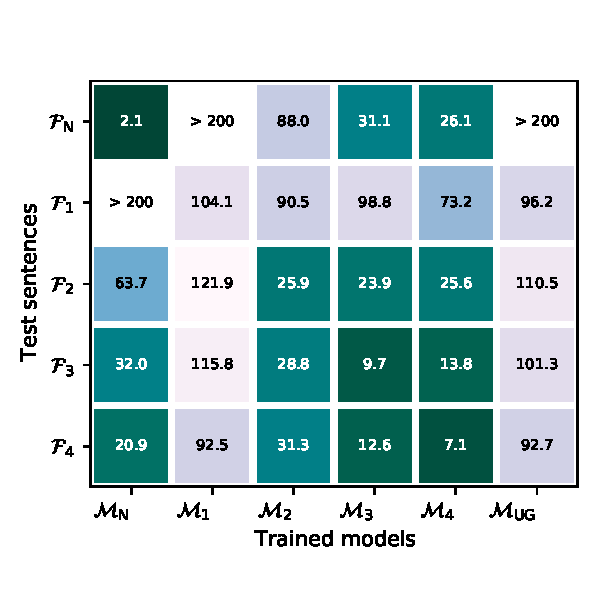
\includegraphics{figs/mlm/bpplm.pdf}}
    \caption{BPPL scores per model per test scenario.}
    \label{fig:bpplm}
\end{figure}

We measure perplexity of various pre-trained randomization models on text that is randomized using the same function $\mathcal{F}$. Conventional language models compute the perplexity of a sentence $S$ by using past tokens ($S_{<t} = (w_1, w_2, \ldots, w_{t-1})$) and the application of chain rule ($\sum_{t=1}^{|S|} \log P_{\textit{LM}}(w_t | S_{t-1})$). However, this formulation is not defined for \acrshort{mlm}, as a word is predicted using the entire sentence as a context.  Following \citet{salazar2020a}, we measure \textit{Pseudo-Perplexity}, i.e., given a sentence $S$, we compute the log-probability of the missing word in $S$ by iteratively masking out the specific word, and computing the average log-probability per word in $S$:

\begin{equation}
    \texttt{PLL}(S) = \frac{1}{|S|} \sum_{w \in S} \log P_{\texttt{\acrshort{mlm}}} (w | S_{\setminus w}; \theta)
\end{equation}

We bootstrap the \texttt{PLL} score of a test corpus $T$ by drawing 100 samples five times with replacement. We also similarly compute the bootstrap perplexity  following \citeauthor{salazar2020a}:

\begin{equation}
    \texttt{BPLL}_{T} = \text{exp}( - \frac{1}{N} \sum_{S \in W} \texttt{PLL}(S)),
\end{equation}

where $W$ is the combined bootstrap sample containing $N$ sentences drawn with replacement from $T$. We compute this score on 6 pre-trained models, over four randomization schemes on the bootstrapped sample $W$ (i.e., we use the same n-gram randomization function $\mathcal{F}_i$). Thus, we obtain a 5x6 matrix of $\texttt{BPLL}$ scores, which we plot in \autoref{fig:bpplm}.

We observe that the pre-trained model \OR\ has the lowest perplexity on the sentences with natural word order. Pre-trained models with random word order exhibit significantly higher perplexity than the normal word order sentences (top row). With the exception of \RI, the models pre-trained on randomized data (\RII, \RIII\ and \RIV) all display the lowest perplexity for their respective $n=2,3,4$ randomizations. %The unigram pre-trained model is a notable exception, which does not yield the lowest perplexity for $n=1$ randomization.
These results indicate that the models  retain and detect the specific word order for which they were trained.

\subsection{The usefulness of word order}
\label{sec:mlm_rda_analysis}

\begin{figure*}[ht]
    \centering
    \resizebox{\textwidth}{!}{
        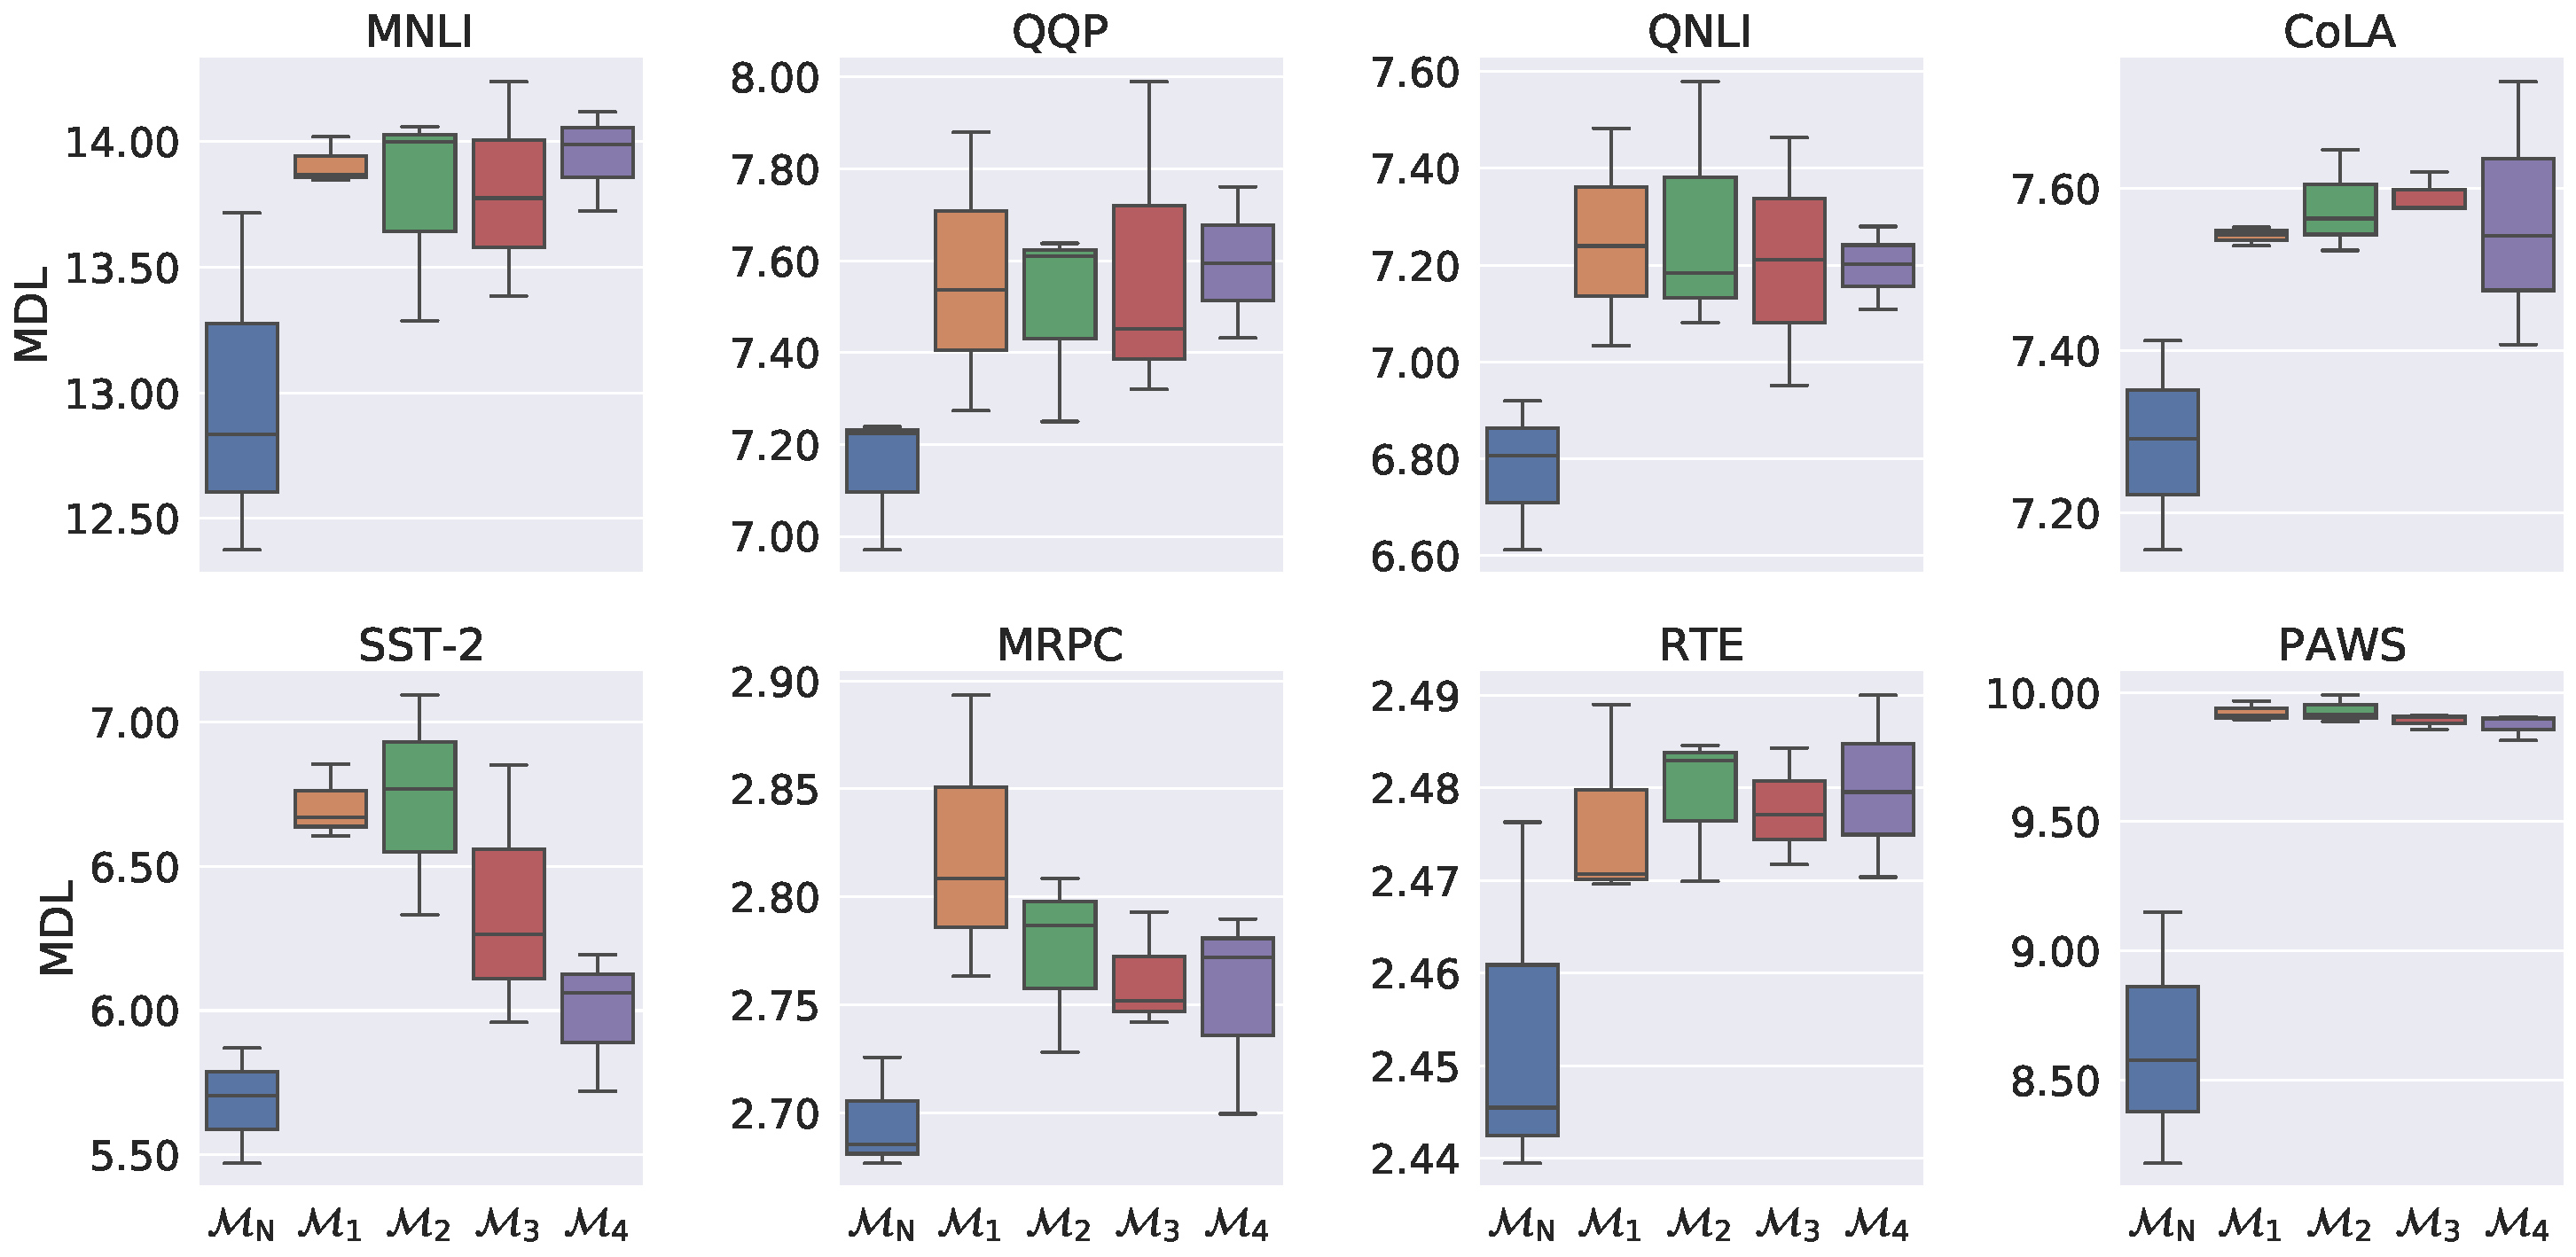
\includegraphics{figs/mlm/rda_mdl_ep_3.pdf}}
    \caption{Rissanen Data Analysis \citep{perez2021} on the GLUE benchmark and PAWS datasets. The lower minimum description length (\acrshort{mdl}, measured in kilobits), the better the learning ability of the model.}
    \label{fig:mlm_rda}
\end{figure*}


The results in \autoref{sec:mlm_glue_results} suggest that, with proper fine-tuning, an unnaturally trained model can reach a level of performance comparable to that of a naturally pre-trained model. However, we want to understand whether natural word order pre-training offers any advantage during the early stages of fine-tuning. Towards that end, we turn to compute the Minimum Description Length \cite[\acrshort{mdl}; ][]{rissanen1984universal}. \acrshort{mdl} is designed to characterize the complexity of data as the length of the shortest program required to generate it. Thus, the length of the minimum description (in bits) should provide a fair estimate of how much word order is useful for fine-tuning in a few-shot setting. Specifically, we leverage the Rissanen Data Analysis (RDA) framework from \citet{perez2021} to evaluate the \acrshort{mdl} of pre-trained models on our set of downstream tasks. Under mild assumptions, if a pre-trained model $\theta_1$ is useful for solving a particular task $T$ over $\theta_2$, then the \acrshort{mdl} in bits obtained by using $\theta_1$ should be shorter than $\theta_2$.
We follow the experimental setup of \citeauthor{perez2021} to compute the \acrshort{mdl} on several tasks using $\theta$ = \{\OR,\RI,\RII,\RIII,\RIV\}, over three seeds and on three epochs of training. Concretely, RDA involves sampling 9 blocks of data from the dataset at random, where the size of each block is increased monotonically, training on 8 blocks while evaluating the model's loss (or \textit{codelength}) on the ninth. The minimum number of data samples in the smallest block is set at 64, while the largest number of data samples used in the last block is 10,000.

We observe that the value of \acrshort{mdl} is consistently lowest for naturally pre-trained data (\autoref{fig:mlm_rda}). For purportedly word order reliant datasets such as RTE, CoLA and PAWS, the gap between the \acrshort{mdl} scores among the natural and unnatural models is high. PAWS, specifically, has the largest advantage in the beginning of optimization, however with more fine-tuning, the model re-learns correct word order (\autoref{sec:mlm_glue_results}). The present analyses, when taken in conjunction with our main results in \autoref{sec:mlm_glue_results}, suggest that fine-tuning on large training datasets with complex classifiers in the pursuit of state-of-the-art results has mostly nullified the impact of word order in the pre-trained representations. Few shot \citep{bansal-etal-2020-learning} and few sample \citep{zhang2021a} learning and evaluation could potentially require more word order signal, thereby encouraging the model to leverage its own learned syntax better.

\subsection{At what point do models learn word order during pre-training?}
% KS: I kind of moved this to appendix as I think the reasoning/ explanation needs to be fleshed out more.

Results from \autoref{sec:mlm_glue_results} beg the question: when, if at all, during pre-training does a model learn the natural word order? We aim to answer that question by comparing downstream task performance of RoBERTa base on intermediate checkpoints with that of the random word order pretrained models. The idea is to find the point during pre-training on natural corpus at which the model exceeds the task performance of the random pre-training model.


\begin{figure}[t]
    \centering
    \resizebox{0.7\textwidth}{!}{
        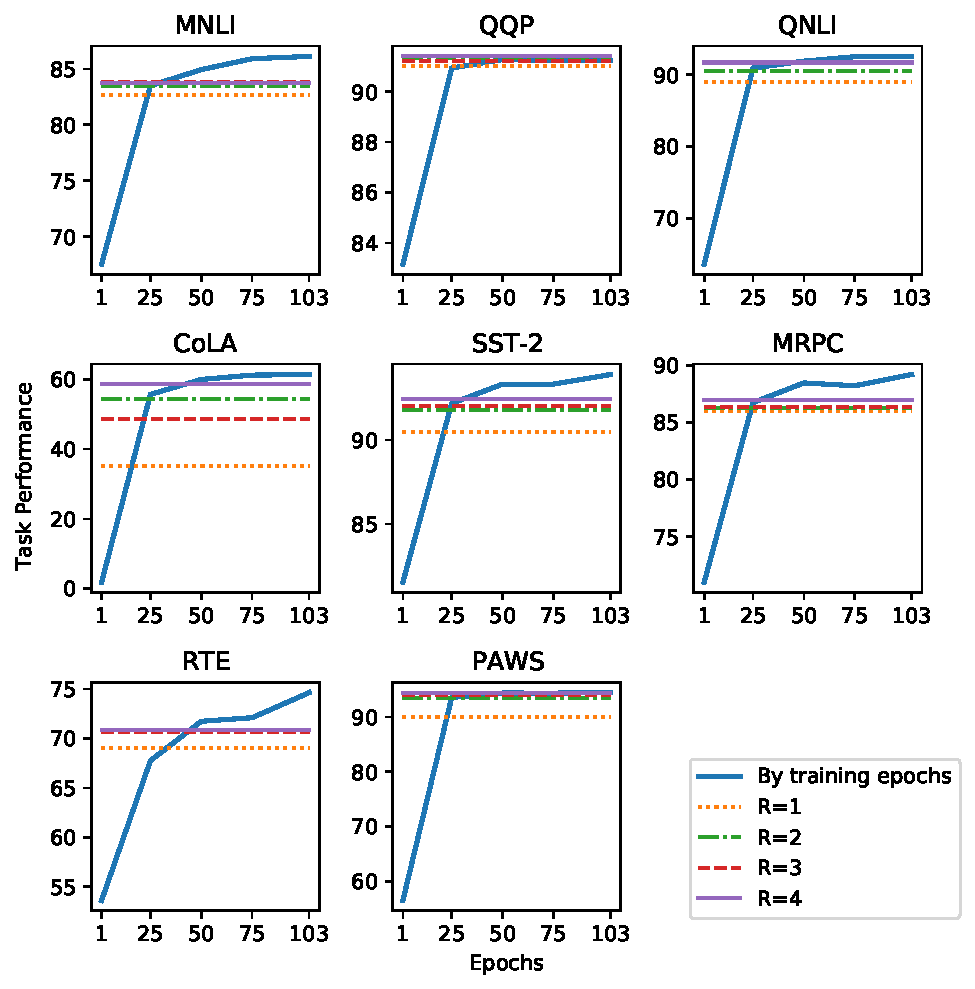
\includegraphics{figs/mlm/glue_progression.pdf}}
    \caption{Comparison among GLUE task performance from different steps in pre-training of RoBERTa on BookWiki Corpus.}
    \label{fig:mlm_glue_progression}
\end{figure}

Performance on all tasks (\autoref{fig:mlm_glue_progression}) increases rapidly during the first 20-25 epochs of pre-training. For some tasks, the word order information only helps after 30-50 pre-training epochs.

\subsection{More results from Syntactic Probes}
\label{sec:mlm_pareto_probes}

\begin{table}[]
\centering
\resizebox{0.7\linewidth}{!}{%
\begin{tabular}{l|rl|rl}
\toprule
Model & \multicolumn{2}{c|}{UD EWT} & \multicolumn{2}{c}{PTB} \\ \hline
 & MLP & Linear & MLP & Linear \\ \cline{2-5} 
\OR & 93.74 +/- 0.15 & 88.82 +/- 0.42 & 97.07 +/- 0.38 & 93.1 +/- 0.65 \\
\midrule
\RI & 88.60 +/- 3.43 & 80.76 +/- 3.38 & 95.33 +/- 0.37 & 87.83 +/- 1.86 \\
\RII & 93.39 +/- 0.45 & 87.58 +/- 1.06 & 96.96 +/- 0.15 & 91.80 +/- 0.50 \\
\RIII & 92.89 +/- 0.65 & 86.78 +/- 1.32 & 97.03 +/- 0.13 & 91.70 +/- 0.70 \\
\RIV & 92.83 +/- 0.61 & 87.23 +/- 0.77 & 96.96 +/- 0.12 & 92.08 +/- 0.39 \\\midrule
\RC & 89.10 +/- 0.21 & 79.75 +/- 0.5 & 94.12 +/- 0.01 & 84.15 +/- 0.51 \\ \bottomrule
\end{tabular}%%
}
\caption{Accuracy on the part-of-speech labelling task (POS) on two datasets, UD EWT and PTB, using the Pareto Probing framework \cite{pimentel-etal-2020-information}.}
\label{tab:pareto_pos_tag}
\end{table}


\begin{table}[t]
\centering
\resizebox{\linewidth}{!}{%
\begin{tabular}{l|rl|rl}
\toprule
Model & \multicolumn{2}{c|}{UD EWT} & \multicolumn{2}{c}{PTB} \\ %\hline
 & MLP & Linear & MLP & Linear \\ \cline{2-5} 
\OR & 89.63 +/- 0.60 & 84.35 +/- 0.78 & 93.96 +/- 0.63 & 88.35 +/- 1.00 \\
\midrule
\RI & 83.55 +/- 3.31 & 75.26 +/- 3.08 & 91.10 +/- 0.38 & 82.34 +/- 1.37 \\
\RII & 88.57 +/- 0.68 & 82.05 +/- 1.10 & 93.27 +/- 0.26 & 86.88 +/- 0.87 \\
\RIII & 88.69 +/- 1.09 & 82.37 +/- 1.26 & 93.46 +/- 0.29 & 87.12 +/- 0.72 \\
\RIV & 88.66 +/- 0.76 & 82.58 +/- 1.04 & 93.49 +/- 0.33 & 87.30 +/- 0.79 \\\midrule
\RC & 84.93 +/- 0.34 & 76.30 +/- 0.52 & 89.98 +/- 0.43 & 78.59 +/- 0.68 \\ \bottomrule
\end{tabular}%%
}
\caption{Accuracy on the dependency arc labelling task (DAL) on two datasets (with mean and std dev), UD EWT and PTB, using the Pareto Probing framework \cite{pimentel-etal-2020-pareto}.}
\label{tab:pareto_dep_label}
\end{table}

\begin{table}[]
\centering
\resizebox{0.6\linewidth}{!}{%
\begin{tabular}{l|l|l}
\toprule
Model & UD EWT & PTB \\ \hline
\OR & 0.528 +/- 0.01 & 0.682 +/- 0.01  \\\midrule
\RI & 0.489 +/- 0.03 & 0.648 +/- 0.01  \\
\RII & 0.529 +/- 0.00 & 0.681 +/- 0.01  \\
\RIII & 0.528 +/- 0.02 & 0.689 +/- 0.01  \\
\RIV & 0.525 +/- 0.00 & 0.683 +/- 0.01  \\\midrule
\RC & 0.510 +/- 0.01 & 0.640 +/- 0.05  \\
\bottomrule
\end{tabular}%
}
\caption{Pareto Hypervolume of dependency parsing task (DEP) on two datasets (with mean and std dev), UD EWT and PTB, using the Pareto Probing framework \cite{pimentel-etal-2020-information}.}
\label{tab:pareto_hypervolume}
\end{table}


%As suggested in \citet{pimentel-etal-2020-pareto}, w
We computed the Pareto Hypervolume on the dependency parsing task \citep{pimentel-etal-2020-pareto}. The Pareto Hypervolume is computed as the Area Under Curve (AUC) score over all hyperparameter runs, where the models are arranged based on their complexity. We observe minimal differences in the Pareto Hypervolumes (\autoref{tab:pareto_hypervolume}) among \OR\ and the randomization models for both datasets.

We also investigated two ``easy'' tasks, Part-of-Speech tagging (POS) and Dependency Arc Labeling (DAL) from the Pareto Probing framework.
For POS (\autoref{tab:pareto_pos_tag}) and DAL (\autoref{tab:pareto_dep_label}), since these tasks are simpler than DEP, the gap between \OR\ and unnaturally pre-trained models reduces even more drastically. The gap between \OR\ and \RI\ reduces to just 3.5 points on average for PTB in both POS and DAL.

\subsection{Non parametric probes}
\label{sec:mlm_non_par_probes}

\begin{figure}[h]
    \centering
    \resizebox{0.8\linewidth}{!}{
        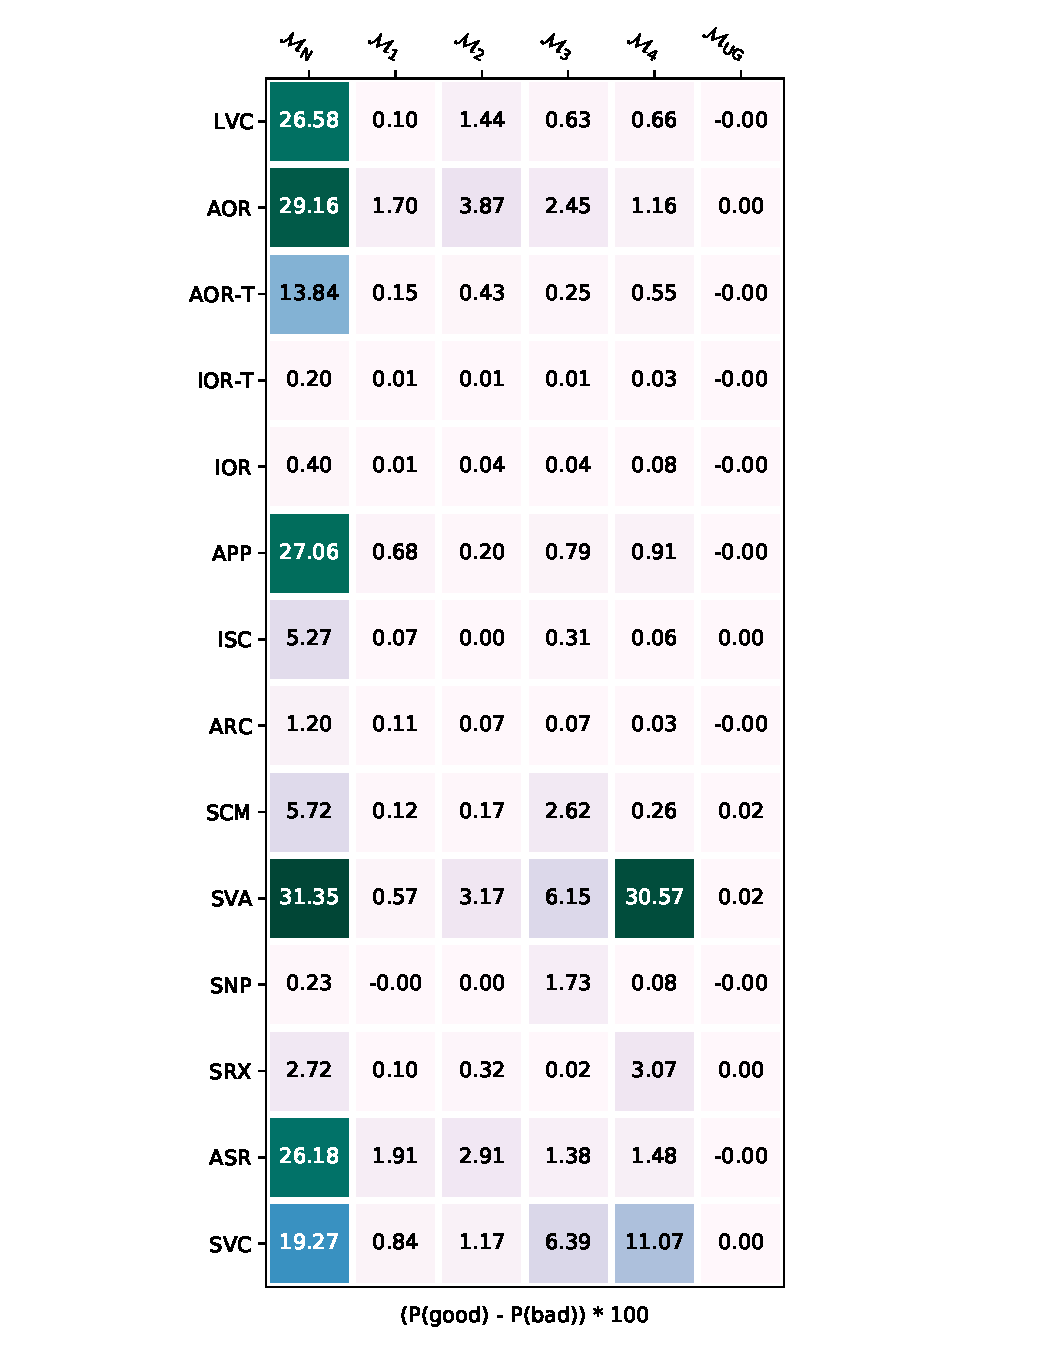
\includegraphics{figs/mlm/non_param_marv_diff.pdf}}
    \caption{The difference in word probabilities for stimuli in \citet{marvin-linzen-2018-targeted}: Simple Verb Agreement (SVA), In a sentential complement (SCM), Short VP Coordination (SVC), Long VP Coordination (LVC), Across a prepositional phrase (APP), Across a subject relative clause (ASR), Across an object relative clause (AOR), Across an object relative (no \textit{that}) (AOR-T),
    In an object relative clause (IOR),
    In an object relative clause (no \textit{that}) (IOR-T),
    Simple Reflexive (SRX), In a sentential complement (ISC),
    Across a relative clause (ARC), Simple NPI (SNP). }
    \label{fig:mlm_marv_diff}
\end{figure}


\xhdr{Probability difference} In the original formulation \citep{goldberg2019assessing, wolf2019}, the effectiveness of each stimulus is determined by the accuracy metric, computed as the number of times the probability of the correct focus word is greater than that of the incorrect word ($P(\textrm{good}) > P(\textrm{bad})$). We observed that this metric might not be reliable per se, since the probabilities may themselves be extremely low for all tokens, even when focus word probability decreases drastically from \OR\ to \RC.
Thus, we also report the mean difference of probabilities, $(\frac{1}{N}\sum_{i}^N P(\textrm{good}_i) - P(\textrm{bad}_i))$, scaled up by a factor of 100 for ease of observation, in \autoref{fig:mlm_gul_diff}, \autoref{fig:mlm_linzen_diff} and \autoref{fig:mlm_marv_diff}.
We observe the highest difference between probabilities of the correct and incorrect focus words for the model pretrained on the natural word order (\OR). Moreover, with each step from \RI\ to \RIV, the difference between probablities of correct and incorrect focus words increases, albeit marginally, showing that pre-trained models with fewer n-gram words perturbed capture more word order information. \RC, the model with the distributional prior ablated, performs the worst, as expected.

\begin{table*}
  \centering
  \resizebox{\linewidth}{!}{%
\begin{tabular}{lllllll}
\toprule
model & \OR & \RC & \RI & \RII & \RIII & \RIV \\
condition &               &                      &                   &                   &                   &                   \\
\midrule
1         &  93.45 (0.89) [25.04] &   58.87 (0.41) [0.0] &  59.96 (1.58) [0.08] &   63.63 (0.6) [1.25] &   64.7 (1.44) [2.79] &   70.47 (1.9) [4.01] \\
2         &    92.8 (1.22) [23.8] &  63.03 (1.35) [0.01] &   58.22 (1.5) [0.09] &  61.15 (2.07) [0.82] &  63.84 (2.41) [2.09] &   64.7 (1.92) [3.07] \\
3         &  87.71 (1.34) [22.03] &   64.06 (3.52) [0.0] &  56.69 (2.98) [0.03] &  56.83 (3.63) [0.85] &   61.1 (0.32) [2.02] &   63.0 (3.36) [2.35] \\
4         &  92.67 (0.52) [22.16] &   76.33 (1.38) [0.0] &  62.33 (7.61) [0.08] &  63.17 (9.09) [1.12] &   69.42 (1.77) [2.1] &  67.67 (7.02) [3.43] \\
\bottomrule
\end{tabular}}
\caption{\citet{linzen-etal-2016-assessing} stimuli results in raw accuracy. Values in parenthesis reflect the standard deviation over different seeds of pre-training. Values in square brackets indicate the mean probability difference among correct and incorrect words.}
\label{tab:linzen_full_balanced}
\end{table*}

\begin{table*}
  \centering
  \resizebox{\linewidth}{!}{%
\begin{tabular}{lllllll}
\toprule
model & \OR & \RC & \RI & \RII & \RIII & \RIV \\
condition &               &                      &                   &                   &                   &                   \\
\midrule
0         &   79.42 (5.5) [2.43] &  47.83 (3.76) [-0.0] &   53.67 (1.38) [0.03] &   58.75 (6.38) [0.05] &  63.58 (4.11) [0.14] &   63.75 (3.28) [0.17] \\
1         &  72.83 (4.07) [2.55] &     44.5 (0.5) [0.0] &    70.83 (5.8) [0.02] &  64.83 (1.76) [-0.09] &  71.67 (6.71) [0.21] &    71.5 (2.65) [0.61] \\
2         &   55.56 (0.0) [0.92] &  88.89 (11.11) [0.0] &  81.48 (12.83) [0.03] &   51.85 (6.42) [0.04] &  62.96 (6.42) [0.38] &  74.07 (16.97) [0.61] \\
\bottomrule
\end{tabular}}
\caption{\citet{gulordava2018} stimuli results in raw accuracy.Values in parenthesis reflect the standard deviation over different seeds of pre-training. Values in square brackets indicate the mean probability difference among correct and incorrect words.}
\label{tab:gul_full_balanced}
\end{table*}

\xhdr{Accuracy comparison}
We provide the accuracy as measured by \citet{goldberg2019assessing, wolf2019} on the probing stimuli in \autoref{tab:linzen_full_balanced}, \autoref{tab:gul_full_balanced} and \autoref{tab:marvin_full_balanced}. We also highlight the difference in probability ($P(\textrm{good}) - P(\textrm{bad})$) in the table to provide a more accurate picture. All experiments were conducted on three pre-trained seeds for each model in our set of models. However, the low token probabilities in \RC\ tend to present unreliable scores. For example, in the case of \citet{gulordava-etal-2018-colorless} stimuli, unnatural models provide better scores compared to the natural model. We also observe for the \citet{linzen-etal-2016-assessing} stimuli that the results on model condition 4 (number of attractors) are surprisingly high for \RC\, whereas the individual token probabilities are lowest. We believe these inconsistencies stem from extremely low token probabilities themselves.  %\citet{gulordava-etal-2018-colorless} typically test on ``\textit{Colorless green ideas}" words, where the probability of a random word with the same POS tag is evaluated for the correct position.

\begin{figure}[]
    \centering
    \resizebox{0.7\linewidth}{!}{
        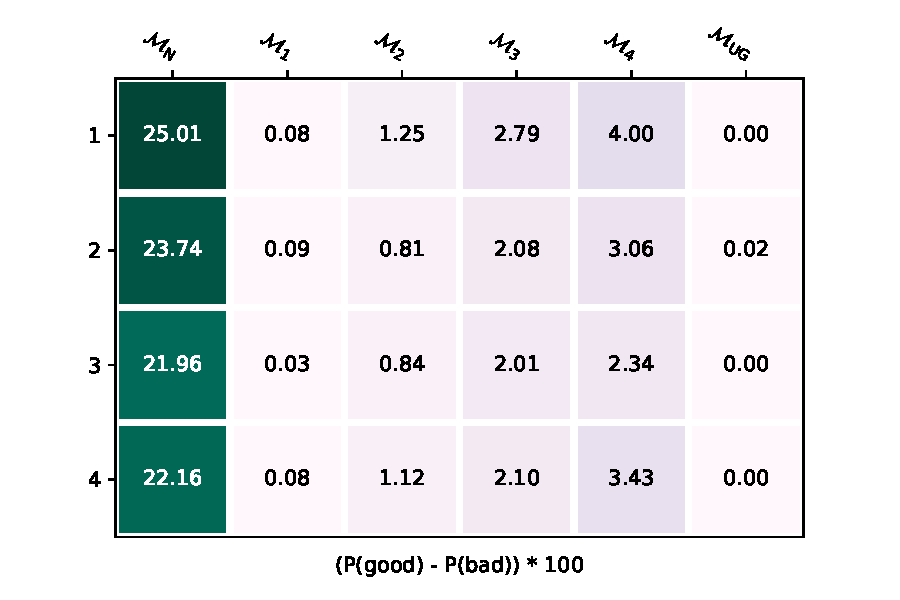
\includegraphics{figs/mlm/non_param_lgd_diff.pdf}}
    \caption{\citet{linzen-etal-2016-assessing}}
    \label{fig:mlm_linzen_diff}
\end{figure}


\begin{figure}[h]
    \centering
    \resizebox{0.7\linewidth}{!}{
        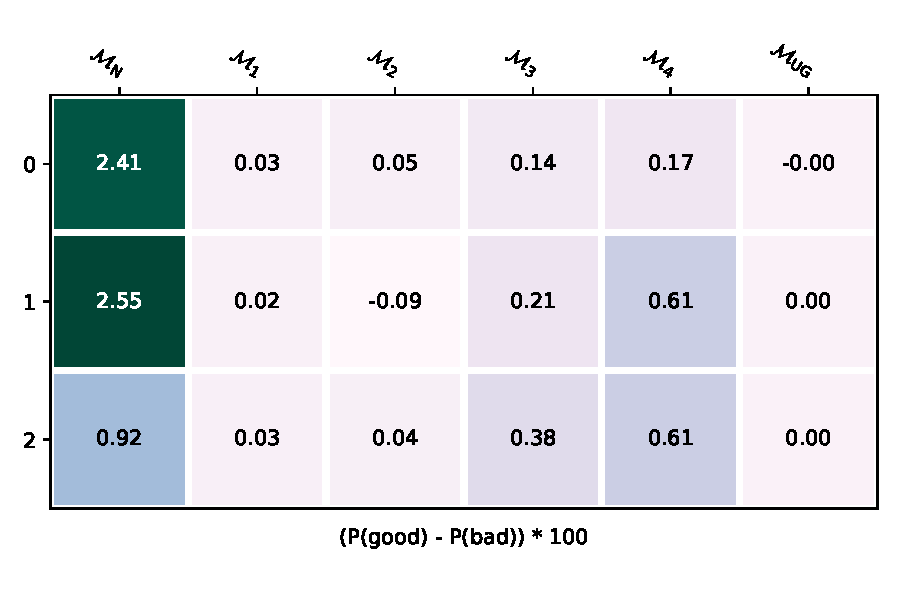
\includegraphics{figs/mlm/non_param_gul_diff.pdf}}
    \caption{\citet{gulordava-etal-2018-colorless}}
    \label{fig:mlm_gul_diff}
\end{figure}

\xhdr{Balancing datasets on inflection by upsampling}
The stimuli datasets of \citet{linzen-etal-2016-assessing} and \citet{gulordava-etal-2018-colorless} turned out to be heavily skewed towards words where singular was the correct inflection (as opposed to plural). This dataset imbalance caused the weak models (such as \RC) to have surprisingly high scores - the weak models were consistently providing higher probability for the singular inflection (\autoref{tab:linzen_full_unbalanced}). We upsample for both datasets, balancing the frequency of correct singular and plural inflections. We compute the upsampling number to the next multiple of 100 of the count of original singular inflections. For example, in condition 4 of \citet{linzen-etal-2016-assessing} dataset, we upsample both S and P to 300 rows each. This type of balancing via upsampling largely alleviated the inconsistencies we observed, and might prove to be useful when evaluating other models on these datasets in future.

\begin{table*}
  \centering
  \resizebox{\linewidth}{!}{%
\begin{tabular}{lllllll}
\toprule
Model &  \OR & \RC & \RI & \RII & \RIII & \RIV \\
condition &                &                      &                   &                   &                   &                   \\
\midrule
AOR       &  89.98 (1.96) [29.16] &    50.0 (0.01) [0.0] &    60.17 (1.61) [1.7] &    66.61 (7.1) [3.87] &  63.57 (2.39) [2.45] &   61.26 (4.91) [1.16] \\
AOR-T     &   77.4 (7.74) [13.84] &     50.0 (0.0) [0.0] &   78.88 (0.64) [0.15] &   52.17 (2.14) [0.43] &   48.85 (3.8) [0.25] &   57.06 (3.49) [0.55] \\
APP       &  89.94 (4.16) [27.06] &  50.01 (0.02) [-0.0] &    70.34 (1.9) [0.68] &     53.61 (3.3) [0.2] &  53.03 (1.75) [0.79] &    60.6 (4.41) [0.91] \\
ARC       &    85.06 (5.92) [1.2] &  50.05 (0.08) [-0.0] &   62.39 (1.91) [0.11] &   74.57 (5.99) [0.07] &  67.55 (3.84) [0.07] &   62.88 (3.45) [0.03] \\
ASR       &  87.19 (3.58) [26.18] &    50.0 (0.0) [-0.0] &  78.55 (10.01) [1.91] &    81.73 (5.1) [2.91] &   62.8 (0.35) [1.38] &   67.23 (6.82) [1.48] \\
IOR       &    89.83 (3.33) [0.4] &  50.55 (0.95) [-0.0] &   56.28 (2.66) [0.01] &   58.96 (4.28) [0.04] &   70.49 (2.2) [0.04] &   62.82 (8.51) [0.08] \\
IOR-T     &    74.05 (8.26) [0.2] &  50.61 (1.05) [-0.0] &   52.63 (2.07) [0.01] &   57.35 (4.88) [0.01] &  61.85 (4.75) [0.01] &   55.16 (6.59) [0.03] \\
ISC       &    85.87 (9.6) [5.27] &     50.0 (0.0) [0.0] &   67.85 (2.62) [0.07] &    82.66 (9.43) [0.0] &  77.69 (4.51) [0.31] &   68.65 (5.71) [0.06] \\
LVC       &   93.0 (0.75) [26.58] &  49.92 (0.14) [-0.0] &    70.42 (6.79) [0.1] &    87.5 (7.26) [1.44] &  85.42 (3.84) [0.63] &   81.08 (5.13) [0.66] \\
SCM       &    88.6 (3.49) [5.72] &    50.0 (0.0) [0.02] &   63.73 (7.94) [0.12] &   82.12 (0.92) [0.17] &  86.44 (3.67) [2.62] &   80.27 (2.46) [0.26] \\
SRX       &    91.0 (6.07) [2.72] &     50.0 (0.0) [0.0] &    88.0 (10.11) [0.1] &  92.25 (10.27) [0.32] &  94.25 (5.02) [0.02] &     91.0 (6.5) [3.07] \\
SVA       &  95.33 (7.23) [31.35] &    50.0 (0.0) [0.02] &    86.0 (5.29) [0.57] &  85.17 (12.87) [3.17] &  94.67 (5.25) [6.15] &  88.83 (9.57) [30.57] \\
SVC       &  97.54 (1.58) [19.27] &    50.0 (0.0) [-0.0] &   83.58 (4.58) [0.84] &   83.71 (8.78) [1.17] &   93.29 (7.4) [6.39] &  81.04 (3.66) [11.07] \\
\bottomrule
\end{tabular}}
\caption{\citet{marvin-linzen-2018-targeted} stimuli results in raw accuracy. Values in parenthesis reflect the standard deviation over different seeds of pre-training. Values in square brackets indicate the mean probability difference among correct and incorrect words. Abbreviations: Simple Verb Agreement (SVA), In a sentential complement (SCM), Short VP Coordination (SVC), Long VP Coordination (LVC), Across a prepositional phrase (APP), Across a subject relative clause (ASR), Across an object relative clause (AOR), Across an object relative (no \textit{that}) (AOR-T),
    In an object relative clause (IOR),
    In an object relative clause (no \textit{that}) (IOR-T),
    Simple Reflexive (SRX), In a sentential complement (ISC),
    Across a relative clause (ARC), Simple NPI (SNP).}
\label{tab:marvin_full_balanced}
\end{table*}


% \begin{table*}
%   \centering
%   \resizebox{\linewidth}{!}{%
% \begin{tabular}{lllllll}
% \toprule
% Model &               \OR &               \RI &               \RII &               \RIII &               \RIV &               \RC \\
% Condition &                  &                  &                  &                  &                  &                  \\
% \midrule
% 1         &  93.92 (2.5e+01) &   62.1 (7.8e-02) &  64.83 (1.3e+00) &  65.27 (2.8e+00) &  70.79 (4.0e+00) &  63.14 (1.6e-03) \\
% 2         &  93.02 (2.4e+01) &  62.86 (8.5e-02) &  62.75 (8.1e-01) &  65.08 (2.1e+00) &  65.44 (3.1e+00) &  71.98 (1.7e-02) \\
% 3         &  88.82 (2.2e+01) &  62.74 (3.4e-02) &  58.99 (8.4e-01) &  63.34 (2.0e+00) &  62.85 (2.3e+00) &  75.71 (3.2e-03) \\
% 4         &  90.53 (2.2e+01) &  63.16 (8.5e-02) &  63.94 (1.1e+00) &  66.41 (2.1e+00) &  66.28 (3.4e+00) &  80.54 (4.0e-03) \\
% \bottomrule
% \end{tabular}}
% \caption{\citet{linzen2016} stimuli results in raw accuracy. Values in parenthesis reflect the $P(\textrm{good}) - P(\textrm{bad})$ metric.}
% \label{tab:linzen_full}
% \end{table*}

\begin{table*}
  \centering
  \resizebox{\linewidth}{!}{%
\begin{tabular}{llllllll}
\toprule
Model &        \OR & \RC &   \RI &   \RII &  \RIII & \RIV & S/P \\
condition &                      &                      &                      &                      &                      &              &        \\
\midrule
1         &   94.04 (0.8) &          62.64 (0.5) &      62.18 (1.33) &      64.91 (0.14) &      65.35 (1.78) &      70.88 (1.88) & 14011 / 10112 \\
2         &  93.28 (0.94) &         71.24 (0.85) &      63.03 (1.69) &      62.92 (2.57) &      65.25 (3.13) &      65.61 (2.35) & 3120 / 1312 \\
3         &   89.1 (0.58) &         74.05 (1.85) &      62.94 (3.13) &      59.18 (3.32) &      63.54 (1.72) &       63.05 (2.0) & 733 / 215 \\
4         &   90.53 (0.9) &         80.03 (0.59) &      63.16 (4.83) &      63.94 (6.92) &      66.41 (3.17) &      66.28 (4.64) & 206 / 51 \\
\bottomrule
\end{tabular}}
\caption{\citet{linzen-etal-2016-assessing} stimuli results in raw accuracy on original, unbalanced data. Values in parenthesis reflect the standard deviation. S/P reflects the count of correct singular and plural focus words.}
\label{tab:linzen_full_unbalanced}
\end{table*}

% \begin{table*}[t]
  \centering
  \resizebox{0.9\linewidth}{!}{%
\begin{tabular}{lrrrrrrrl}
\toprule
Model &  QNLI &   RTE &   QQP &  SST-2 &  MRPC &  CoLA &  PAWS &           MNLI (m/mm) \\
\midrule
   OR & 0.925 & 0.746 & 0.913 &  0.939 & 0.892 & 0.614 & 0.945 &  0.861 / 0.854 \\
   R1 & 0.890 & 0.690 & 0.910 &  0.905 & 0.860 & 0.352 & 0.900 &  0.826 / 0.827 \\
   R2 & 0.904 & 0.708 & 0.914 &  0.918 & 0.862 & 0.544 & 0.935 &  0.834 / 0.835 \\
   R3 & 0.917 & 0.707 & 0.912 &  0.920 & 0.864 & 0.487 & 0.940 &  0.838 / 0.838 \\
   R4 & 0.917 & 0.708 & 0.914 &  0.925 & 0.870 & 0.587 & 0.943 &  0.838 / 0.839 \\ \hline
   RC & 0.711 & 0.540 & 0.855 &  0.834 & 0.705 & 0.000 & 0.585 &  0.719 / 0.715 \\
\bottomrule
\end{tabular}}
\caption{GLUE and PAWS dev set results on RoBERTa (base), trained on variants of BookWiki corpus. We use the same evaluation setup of \citet{liu2019b}, and report the median over 5 seeds for the best hyperparam configuration.}
\label{table:glue}
\end{table*}


% Please add the following required packages to your document preamble:
% \usepackage{booktabs}
% \usepackage{graphicx}
\begin{table*}[]
\centering
\resizebox{\textwidth}{!}{%
\begin{tabular}{|l|p{0.3\linewidth}|p{0.3\linewidth}|p{0.3\linewidth}|p{0.3\linewidth}|p{0.3\linewidth}|}
\toprule
 & OR & R1 & R2 & R3 & R4 \\ \midrule
1 & They are commonly known as daturas, but also known as devil's trumpets, not to be confused with angel's trumpets, its closely related genus "Brugmansia". & be They angel's also but trumpets, genus related devil's as commonly closely known its daturas, trumpets, as "Brugmansia". confused with known are to not & as devil's They genus not to trumpets, closely related "Brugmansia". are commonly trumpets, its also known known as be confused daturas, but with angel's & "Brugmansia". related They are commonly trumpets, its closely as daturas, but known genus also known as trumpets, confused with angel's devil's not to be & its closely related genus They are commonly known trumpets, as trumpets, daturas, but also known as "Brugmansia". not to be confused with angel's devil's \\
2 & They are also sometimes called moonflowers, jimsonweed, devil's weed, hell's bells, thorn-apple, and many more. & are devil's bells, called weed, hell's thorn-apple, and many They also more. moonflowers, jimsonweed, sometimes & more. They are hell's bells, also sometimes and many called moonflowers, jimsonweed, devil's weed, thorn-apple, & jimsonweed, devil's weed, They are also thorn-apple, and many bells, more. hell's sometimes called moonflowers, & moonflowers, They are also sometimes bells, thorn-apple, and many more. called jimsonweed, devil's weed, hell's \\
3 & Its precise and natural distribution is uncertain, owing to its extensive cultivation and naturalization throughout the temperate and tropical regions of the globe. & throughout owing precise extensive temperate and naturalization and tropical of to natural is its Its distribution cultivation the globe. uncertain, regions the and & and natural distribution is tropical to its and naturalization throughout the the temperate and globe. Its precise uncertain, owing extensive cultivation regions of & uncertain, owing to Its precise and its extensive cultivation of globe. natural distribution is the the and tropical regions and naturalization throughout temperate & globe. Its precise and natural cultivation distribution the is uncertain, owing to its extensive and naturalization throughout the temperate and tropical regions of \\
4 & Its distribution within the Americas and North Africa, however, is most likely restricted to the United States, Mexico and Southern Canada in North America, and Tunisia in Africa where the highest species diversity occurs. & distribution Mexico occurs. likely diversity North however, species most the Tunisia where in and and North Canada Southern America, highest Africa United the and in Americas Its within States, is to the restricted Africa, & and Tunisia the Americas distribution within Mexico and is most United States, Africa, however, Africa where in North Its and North in Southern Canada America, the to the likely restricted occurs. highest species diversity & likely Its highest species diversity United States, Mexico restricted to the Africa where the occurs. distribution within the and Tunisia in however, is most Americas and Southern Canada and North Africa, in North America, & Tunisia occurs. Its distribution within the Africa where the highest in restricted to the United Canada in North America, most North Africa, however, is and Americas likely diversity States, Mexico and Southern species and \\
5 & All species of "Datura" are poisonous, especially their seeds and flowers. & seeds and species of poisonous, "Datura" their are All flowers. especially & "Datura" are especially their flowers. seeds and of All species poisonous, & especially their seeds flowers. "Datura" are poisonous, All species of and & flowers. poisonous, species of "Datura" are All especially their seeds and \\
6 & Some South American plants formerly thought of as "Datura" are now treated as belonging to the distinct genus "Brugmansia" ("Brugmansia" differs from "Datura" in that it is woody, making shrubs or small trees, and it has pendulous flowers, rather than erect ones). & and "Datura" treated from than flowers, it small belonging woody, thought as ones). South differs Some "Brugmansia" American as are in the rather pendulous distinct making now erect "Datura" to ("Brugmansia" of formerly trees, or is it that plants genus has shrubs & "Brugmansia" ("Brugmansia" than erect pendulous genus and ones). is woody, small trees, of as the distinct flowers, rather Some South differs from American plants treated as formerly thought belonging to "Datura" in making that it "Datura" are it has now shrubs or & woody, small trees, and has pendulous flowers, as belonging to Some making shrubs or as rather than erect "Datura" are now "Brugmansia" ("Brugmansia" differs the distinct genus from "Datura" in formerly thought of it treated that it is ones). South American plants & belonging to the distinct has making Some ("Brugmansia" differs from "Datura" in are now treated as genus pendulous shrubs flowers, rather than erect or ones). "Brugmansia" that it is woody, South American plants formerly thought of as "Datura" small trees, and it \\
7 & Other related taxa include & taxa Other include related & include Other related taxa & include Other related taxa & Other related taxa include \\
8 & "Hyoscyamus niger", "Atropa belladonna", "Mandragora officinarum", Physalis, and many more. & and many niger", officinarum", belladonna", "Mandragora "Atropa "Hyoscyamus more. Physalis, & belladonna", "Mandragora "Hyoscyamus niger", many Physalis, and more. officinarum", "Atropa & more. Physalis, and many belladonna", "Mandragora officinarum", "Hyoscyamus niger", "Atropa & niger", more. belladonna", "Mandragora officinarum", Physalis, "Atropa many and "Hyoscyamus \\
9 & The name "Datura" is taken from Sanskrit ' 'thorn-apple', ultimately from Sanskrit ' 'white thorn-apple' (referring to "Datura metel" of Asia). & of Asia). taken from name The "Datura" ' is to 'thorn-apple', Sanskrit ' Sanskrit metel" 'white (referring from "Datura thorn-apple' ultimately & "Datura" is taken from to ' 'thorn-apple', Sanskrit ' 'white of thorn-apple' (referring Asia). The name Sanskrit ultimately from "Datura metel" & Sanskrit ' The name "Datura" 'thorn-apple', ultimately from metel" Asia). is taken from of 'white (referring to "Datura Sanskrit ' thorn-apple' & Asia). The name "Datura" is from taken of from Sanskrit ' 'thorn-apple', ultimately Sanskrit ' 'white thorn-apple' (referring to "Datura metel" \\
10 & In the Ayurvedic text Sushruta different species of Datura are also referred to as ' and '. & the of also Sushruta Datura are referred to as In Ayurvedic and different species ' text '. & species of referred to are also Datura Sushruta different and as ' Ayurvedic text In the '. & as ' and In the Ayurvedic also referred to species of Datura are text Sushruta different '. & different In the Ayurvedic text also referred to as and Sushruta ' species of Datura are '. \\ \bottomrule
\end{tabular}%
}
\caption{First 10 lines from the BookWiki corpus, and their respective n-gram permutations.}
\label{tab:sample_permutations}
\end{table*}

\begin{table*}[t]
  \centering
  \resizebox{0.7\linewidth}{!}{%
\begin{tabular}{lrrrrrrrr}
\toprule
        Model &   RTE &  MRPC &  SST-2 &  CoLA &   QQP &  QNLI &  MNLI &  PAWS \\
\midrule
        \OR & 2e-05 & 2e-05 &  1e-05 & 2e-05 & 1e-05 & 1e-05 & 1e-05 & 2e-05 \\
         \RI & 2e-05 & 1e-05 &  1e-05 & 1e-05 & 3e-05 & 1e-05 & 2e-05 & 2e-05 \\
         \RII & 2e-05 & 2e-05 &  1e-05 & 1e-05 & 2e-05 & 1e-05 & 1e-05 & 3e-05 \\
         \RIII & 3e-05 & 1e-05 &  2e-05 & 2e-05 & 3e-05 & 1e-05 & 1e-05 & 2e-05 \\
         \RIV & 3e-05 & 1e-05 &  2e-05 & 2e-05 & 2e-05 & 1e-05 & 1e-05 & 2e-05 \\
         \RV & 1e-05 & 3e-05 &  2e-05 & 2e-05 & 3e-05 & 2e-05 & 3e-05 & 2e-05 \\
 \RC & 2e-05 & 1e-05 &  3e-05 & 1e-05 & 3e-05 & 3e-05 & 3e-05 & 2e-05 \\
\RU & 2e-05 & 1e-05 &  3e-05 & 2e-05 & 3e-05 & 3e-05 & 3e-05 & 1e-05 \\
   \RT & 1e-05 & 1e-05 &  3e-05 & 1e-05 & 1e-05 & 1e-05 & 2e-05 & 1e-05 \\
      \NP & 1e-05 & 3e-05 &  2e-05 & 1e-05 & 1e-05 & 1e-05 & 1e-05 & 1e-05 \\
\bottomrule
\end{tabular}}
\caption{Fine-tuning hyperparam Learning rate of each model for each task in GLUE and PAWS}
\label{table:glue_hyp_lr}
\end{table*}

\begin{table*}[t]
  \centering
  \resizebox{0.7\linewidth}{!}{%
\begin{tabular}{lrrrrrrrr}
\toprule
        Model &  RTE &  MRPC &  SST-2 &  CoLA &  QQP &  QNLI &  MNLI &  PAWS \\
\midrule
        \OR &   16 &    16 &     32 &    16 &   16 &    32 &    32 &    16 \\
         \RI &   32 &    32 &     16 &    32 &   32 &    16 &    32 &    16 \\
         \RII &   32 &    16 &     32 &    16 &   32 &    32 &    16 &    32 \\
         \RIII &   32 &    32 &     16 &    32 &   32 &    16 &    32 &    32 \\
         \RIV &   32 &    16 &     32 &    16 &   32 &    32 &    32 &    32 \\
        \RV &   32 &    16 &     16 &    32 &   32 &    16 &    16 &    16 \\
 \RC &   16 &    16 &     16 &    16 &   32 &    16 &    16 &    32 \\
\RU &   16 &    32 &     16 &    16 &   32 &    16 &    16 &    16 \\
   \RT &   16 &    16 &     32 &    16 &   16 &    16 &    32 &    16 \\
      \NP &   16 &    32 &     16 &    16 &   32 &    16 &    16 &    16 \\
\bottomrule
\end{tabular}
}
\caption{Finetuning hyperparam batch size of each model for each task in GLUE and PAWS}
\label{table:glue_hyp_bs}
\end{table*}



\section{Related Work}
\label{sec:mlm_related_work}


\subsection{Sensitivity to word order in \acrshort{nlu}}

Information order has been a topic of research in computational linguistics since \cite{barzilay-lee-2004-catching} introduced the task of ranking sentence orders
%text-ordering task: algorithm has to select a maximally coherent sentence order from a set of candidate permutations
as an evaluation for language generation quality, an approach which was subsequently also used to evaluate readability and dialogue coherence \citep{barzilay-lapata-2008-modeling, laban-etal-2021-transformer}.

More recently, several research groups have investigated information order for words rather than sentences as an evaluation of model humanlikeness. %\citet{sinha2020b}, \citet{pham-etal-2020-out}, and \citet{gupta-etal-2021-bert}.
In our previous chapter (Chapter \autoref{sec:unli}), we investigate the task of natural language inference (NLI) and find high accuracy on permuted examples for different Transformer and pre-Transformer era models, across English and Chinese datasets \citep{hu-etal-2020-ocnli}.
\citet{gupta-etal-2021-bert} use targeted permutations on RoBERTa-based models and show word order insensitivity across natural language inference (MNLI), paraphrase detection (QQP) and sentiment analysis tasks (SST-2).
%RoBERTa has been found to assign high confidence to targeted permutations, even with drastic changes in word order.
\citet{pham-etal-2020-out} show insensitivity on a larger set of tasks, including the entire GLUE benchmark, and find that certain tasks in GLUE, such as CoLA and RTE are more sensitive to permutations than others.
\cite{ettinger-2020-whatbertisnot} recently observed that BERT accuracy decreases for some word order perturbed examples, but not for others.
In all these prior works, models were given access to normal word order at (pre-)training time, but not at fine-tuning or test time. It was not clear whether the model acquires enough information about word order during the fine-tuning step, or whether it is ingrained in the pre-trained model.
% This could mean that models' achieve high accuracy on test datasets because the information about word order learned from standard pre-training outweighs what is learned from fine-tuning on permuted data.
In this work, we take these investigations a step further: we show that the word order information needed for downstream tasks does not need to be provided to the model during pre-training. Since models can learn whatever word order information they do need largely from fine-tuning alone, this likely suggests that our downstream tasks don't actually require much complex word order information in the first place (cf.,\ \citealt{glavas-vulic-2021-supervised}).
% and show that training on word order permuted sentences only degrades test set accuracy somewhat - some important word order information can be learned solely from normal-order fine-tuning (cf.\ \citealt{howard-ruder-2018-universal}).

\subsection{Randomization ablations}

Random controls have been explored in a variety of prior work.
\citet{wietingkiela2019} show that random sentence encoders are surprisingly powerful baselines.  \citet{gauthier-levy-2019-linking} use random sentence reordering to label some tasks as ``syntax-light'' making them more easily decodeable from images of the brain.
\citet{shen2020a} show that entire layers of \acrshort{mlm} transformers can be randomly initialized and kept frozen throughout training without detrimental effect and that those layers perform better on some probing tasks than their frozen counterparts.
Models have been found to be surprisingly robust to randomizing or cutting syntactic tree structures they were hoped to rely on~\cite{scheible2013cutting,williams2018latent}, and randomly permuting attention weights often induces only minimal changes in output \cite{jain-wallace-2019-attention}. In computer vision, it is well known that certain architectures constitute good ``deep image priors'' for fine-tuning~\cite{ulyanov2018deep} or pruning~\cite{frankle2020training}, and that even randomly wired networks can perform well at image recognition~\cite{xie2019exploring}. Here, we explore randomizing the data, rather than the model, to assess whether certain claims about which phenomena the model has learned are established in fact.

% Commenting this section out as per suggestion by Dieuwke

\subsection{Synthetic pre-training}

\citet{kataoka2021} found that pre-training on synthetically generated fractals for image classification is a very strong prior for subsequent fine-tuning on real image data. In language modeling, \citet{papadimitriou-jurafsky-2020-learning} train LSTMs \citep{hochreiter1997long} on non-linguistic data with latent structure such as MIDI music or Java code provides better test performance on downstream tasks than a randomly initialized model. They observe that even when there is no vocabulary overlap among source and target languages, LSTM language models leverage the latent hierarchical structure of the input to obtain better performance than a random, Zipfian corpus of the same vocabulary.


\subsection{On the utility of probing tasks}

Many recent papers provide compelling evidence that BERT contains a surprising amount of syntax, semantics, and world knowledge \citep{giulianelli-etal-2018-hood,rogers-etal-2020-primer,lakretz-etal-2019-emergence,jumelet-etal-2019-analysing,jumelet-etal-2021-language}. Many of these works involve diagnostic classifiers \citep{hupkes2018visualisation} or \textit{parametric} probes, i.e.\ a function atop learned representations that is optimized to find linguistic information. How well the probe learns a given signal can be seen as a proxy for linguistic knowledge encoded in the representations. % \citep{hupkes2018visualisation}
However, the community is divided on many aspects of probing \citep{belinkov2021probing} including how complex probes should be.
Many prefer \textit{simple} linear probes over the complex ones \citep{alain2016understanding, hewitt-manning-2019-structural, hall-maudslay-etal-2020-tale}. However, complex probes with strong representational capacity are able to extract the most information from representations \citep{voita-titov-2020-information, pimentel-etal-2020-information, hall-maudslay-etal-2020-tale}.
% On the one hand, proponents of \textit{simple} linear probes argue that having explicit, focused classifiers should provide better signal as the function itself is too weak on its own \citep{alain2016understanding, hewitt-manning-2019-structural, hall-maudslay-etal-2020-tale}. On the other hand, proponents of \textit{complex} probes claim that having strong representational capacity of the probe is actually helpful for extracting the most information from a representation \citep{pimentel2020}. There are also strong calls from the community to use information theoretic approaches instead of accuracy \citep{voita-titov-2020-information, pimentel2020}, as well  harder \textit{tasks} for probing \citep{hall-maudslay-etal-2020-tale, pimentel-etal-2020-pareto}.
In this chapter, we follow \citet{pimentel-etal-2020-pareto} and use \textit{both} simple (linear) and complex (non-linear) models, as well as ``complex'' tasks (dependency parsing).
As an alternative to parametric probes,  stimulus-based \textit{non-parametric} probing \citep{linzen-etal-2016-assessing, jumelet-hupkes-2018-language, marvin-linzen-2018-targeted, gulordava-etal-2018-colorless, warstadt-etal-2019-investigating,ettinger-2020-whatbertisnot,lakretz2021mechanisms,warstadt-etal-2020-blimp,warstadt-etal-2020-learning} has been used to show that even without a learned probe, BERT can predict syntactic properties with high confidence~\citep{goldberg2019assessing, wolf2019}.
%Stimulus-based probing is also sometimes called \textit{non-parametric}, since no additional parameters need to be learned to probe with this method.
We use this class of non-parametric probes to investigate RoBERTa's ability to learn word order during pre-training.



\section{Discussion}
\label{sec:mlm_discussion}

The assumption that word order information is crucial for any classical NLP pipeline (especially for English) is deeply ingrained in our understanding of syntax itself \citep{chomsky1957syntactic}: without order, many linguistic constructs are undefined. (e.g.\ dependency or constituency parses would no longer be syntactic trees, what would sentences be but mere lists of words).
Our fine-tuning results in \autoref{sec:mlm_glue_results} and parametric probing results in \autoref{sec:mlm_param_probing}, however, suggests that \acrshort{mlm}s do not need to rely much on word order to achieve high accuracy, bringing into question previous claims that they learn a ``classical NLP pipeline.''

% The assumption that word order information is crucial for any classical NLP pipeline (especially for English) is deeply ingrained in our understanding of syntax itself \citep{chomsky1957syntactic}: without order, most linguistic constructs are undefined

One might ask, though, whether an NLP pipeline would really need natural word order at all: can transformers not simply learn what the correct word order is from unordered text?
First, the lower non-parametric probing accuracies of the randomized models indicate that they are not able to accurately reconstruct the original word order (see also \autoref{sec:mlm_ablations}).
But even if models were able to ``unshuffle'' the words under our unnatural pre-training set up, they would only be doing so based on distributional information.
Models would then abductively learn only the most likely word order. %---as evidenced by the effectiveness of the distributional prior alone in achieving good enough fine-tuning and probing performance, high perplexity for randomized models on the original data, and our non-parametric probing results. % showing that these models cannot recover word order nearly as well.
While models might infer a distribution over possible orders and use that information to structure their representations \citep{papadimitriou-etal-2021-deep}, syntax is not about \emph{possible} or even  \emph{the most likely} orders: it is about the \emph{actual} order. That is, even if one concludes in the end that Transformers are able to perform word order reconstruction based on distributional information, and recover almost all downstream performance based solely on that, we ought to be a lot more careful when making claims about what our evaluation datasets are telling us.

Thus, our results seem to suggest that we may need to revisit what we mean by ``linguistic structure,'' and perhaps subsequently acknowledge that we may not need human-like linguistic abilities for most NLP tasks. Or, our results can be interpreted as evidence that we need to develop more challenging and more comprehensive evaluations%
%(cf. \citealt{bowman2021will})
, if we genuinely want to measure linguistic abilities, however those are defined, in NLP models.

% There are many interesting and potentially exciting avenues for future work that we could not explore due to limitation of space. An interesting question revolves around whether this phenomenon is more pronounced for English than for other languages. It is natural to wonder whether more word-order flexible or morphologically-rich languages would suffer from the same problem. Using the methods discussed in this work, we could imagine devising a way to determine the degree of order-dependence for tasks across languages. Another possible extension pertains to other tasks, including extractive question answering (QA) or sequence tagging, for which we can also to determine whether word order information is acquired downstream or during pre-training.

To summarize, in this chapter, we revisited the hypothesis that masked language modelling's impressive performance can be explained in part by its ability to learn classical NLP pipelines. We investigated targeted pre-training on sentences with various degrees of randomization in their word order, and observed overwhelmingly that \acrshort{mlm}'s success is most likely not due to its ability to discover syntactic and semantic mechanisms necessary for a traditional language processing pipeline during pre-training. Instead, our experiments suggest that \acrshort{mlm}'s success can largely be explained by it having learned higher-order distributional statistics that make for a useful prior for subsequent fine-tuning. These results should hopefully encourage the development of better, more challenging tasks that require sophisticated reasoning, and harder probes to narrow down what exact linguistic information is present in the representations learned by our models.
%


% \section{Follow-up findings in the community}
% \label{sec:mlm_followup}

% Our work in this chapter involving surprising word-order insensitivity of \acrshort{mlm} models during pre-training has garnered significant interest in the community since its publication in 2021. In this section I highlight some of the interesting publications following the results from our work.

% \citet{Chiang2022OnTT}

% \citet{taktasheva-etal-2021-shaking}

\clearpage
\chapter{Measuring systematic generalization by exploiting absolute positions}
\label{sec:pos}

Recently, Transformer \citep{vaswani-etal-2017-attention} language models (TLMs) have been widely used for natural language applications. Such models incorporate positional encodings: vectors encoding information about the order of words in context. Many models, such as RoBERTa \citep{liu-et-al-2019-roberta}, GPT3 \citep{Brown2020:GPT3} and OPT \citep{Zhang2022:OPT}, utilize \textit{absolute} position embeddings (\acrshort{ape}s) that directly encode absolute (linear) word order. \acrshort{ape}s appear to contribute to the performance of such models.

However, in our previous chapters (\autoref{sec:unli} and \autoref{sec:mlm}), we observe models lack a sense of relative positions, as they become (in)sensitive to ablative word scrambles. Furthermore, recent studies have shown that removing \acrshort{ape}'s seem to work optimally \citep{haviv2022}. Thus, what precisely \acrshort{ape}s contribute remains unclear.

It is conceivable that \acrshort{ape}s may enable the model to handle the relative distances between words. % Using embeddings that explicitly encode relative distance have been found to improve performance on machine translation \citep{shaw-etal-2018-self}, although they are somewhat less space inefficient \citep{velickovic-etal-2018-graph} than their absolute counterparts.
If models were somehow learning relative position information despite using \emph{absolute} positional embeddings, we would expect sentence encodings to be the same in most cases, regardless of where they appear in the context window. For example, the meaning of ``smoking kills'' should be constant in ``Kim said \textit{smoking kills}'' (positions 2--3)  and ``It was commonly believed by most adult Americans in the 90s that \textit{smoking kills}'' (positions 13--14), despite the fact that these words appear in different absolute positions.
% These findings encourage further investigation on one specific component of TLMs, which are often overlooked: the role of position embeddings.
% In this work, we revisit the role of \acrshort{ape}s, a class of position embeddings which are typically learned during pre-training.
Given this, our central question is: do \acrshort{ape}s enable the model to learn the relative distances between the words in a sentence?

Prior work has attempted to explore the consequences of \acrshort{ape}s using probing methods \citep{wang2021on}.
\acrshort{ape}s have been found to not capture the meaning of absolute or relative positions \citep{wang-chen-2020-position}.
\acrshort{ape}s have also been found to bias model output with positional artefacts \citep{luo-etal-2021-positional}, leading to better performance on token to position de-correlation \citep{ke2021}.
\citet{haviv2022} even find that causal TLMs perform adequately even without an explicit \acrshort{ape}s.
%For instance, \citet{wang2021on} establish key required properties of \acrshort{ape}s involving monotonicity, translation and symmetry.
However, a systematic study on relativity of positional encodings is still needed.

% \KS{insert representative image}
\begin{figure}
    \centering
    \resizebox{\linewidth}{!}{
    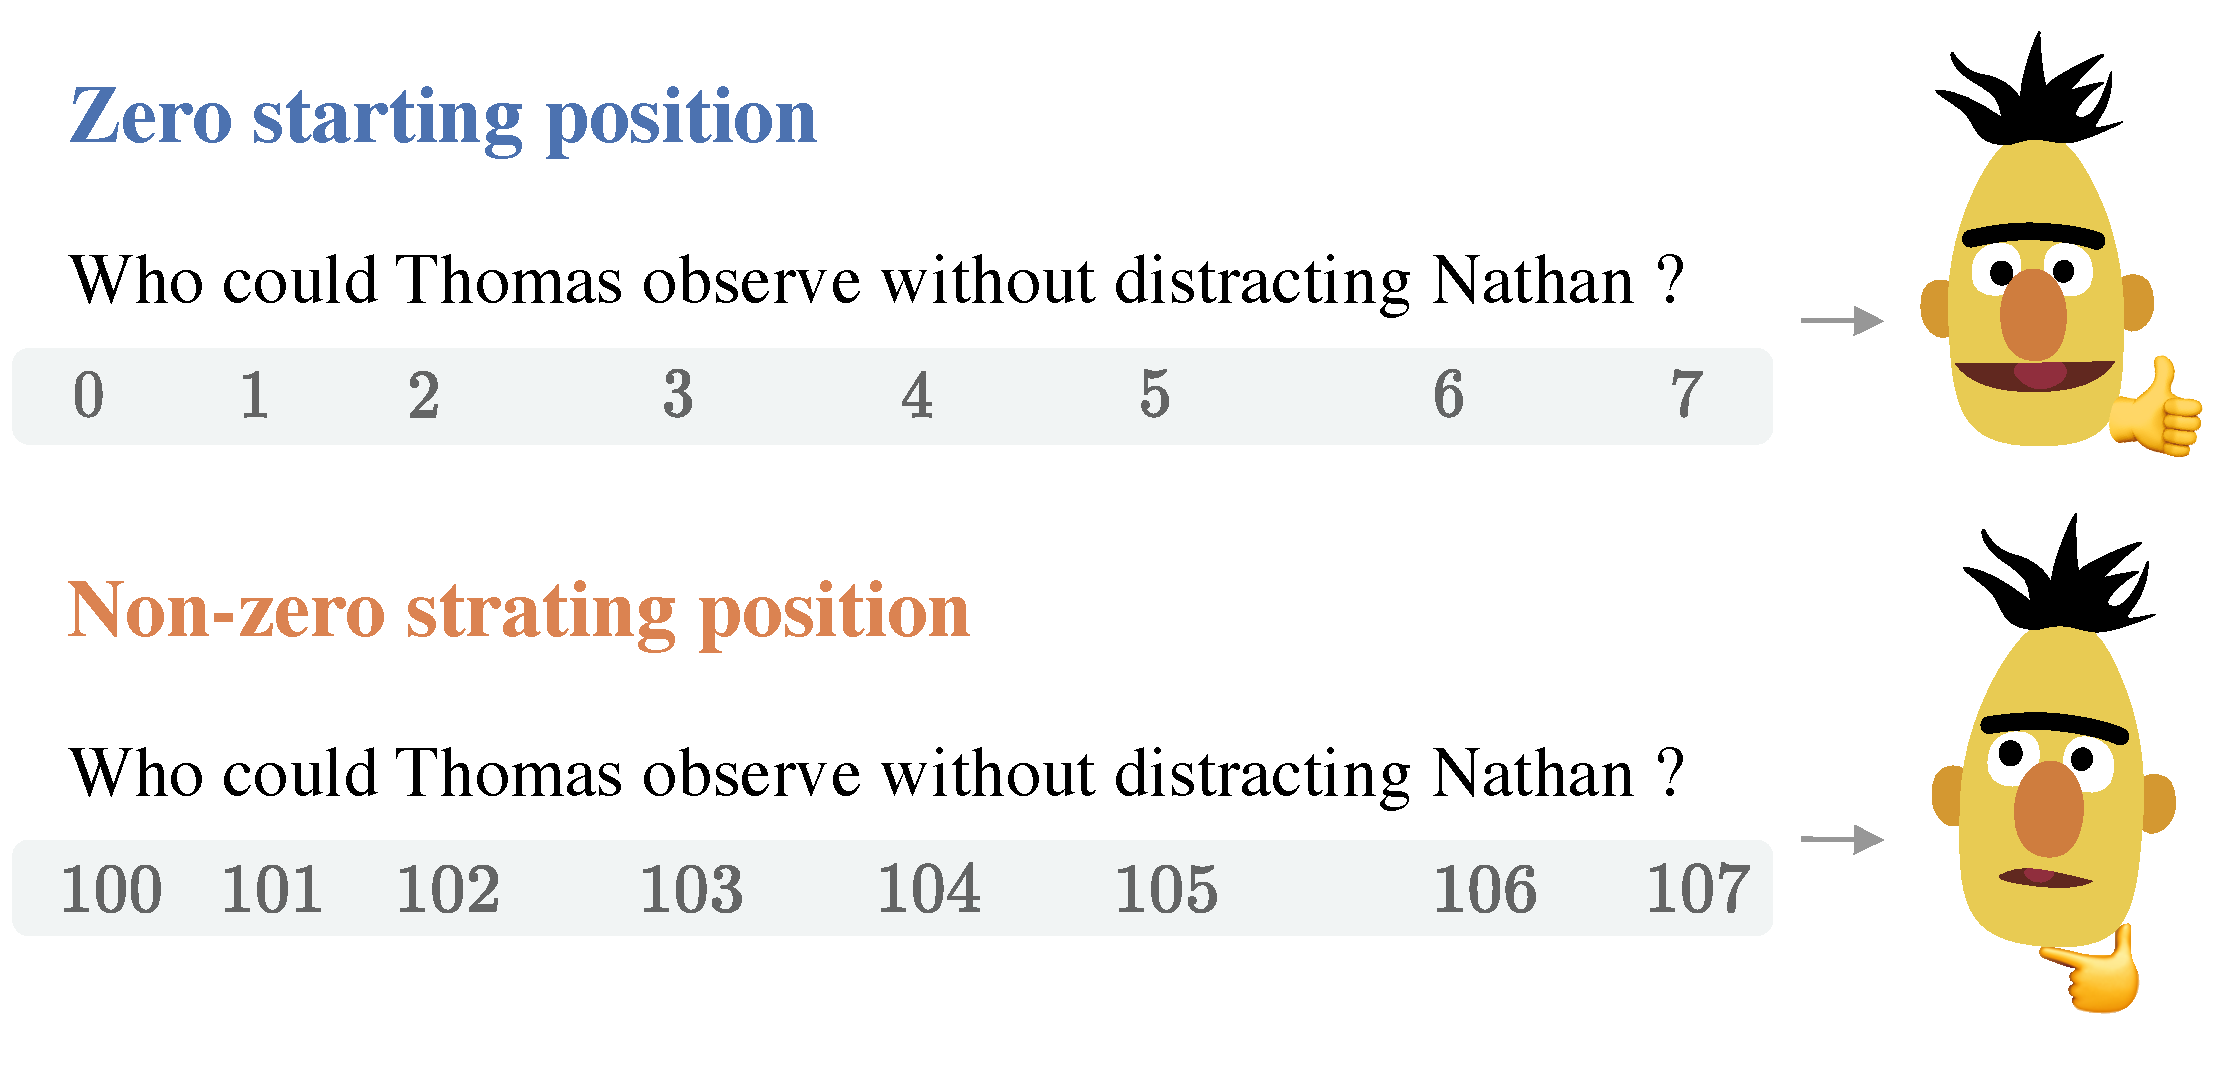
\includegraphics[width=\textwidth]{figs/pos/bert_confused.pdf}}
    \caption{Transformer models with absolute positional embeddings have different representations for sentences starting from non-zero positions. }
    \label{fig:bert_confused}
\end{figure}

% We argue \acrshort{ape}s on various downstream tasks might answer the question as yes, but it obfuscates position importance with task-level token associations.
% Transformer models are usually trained in a batch containing multiple sentences, with a fixed window size of maximum tokens per batch element, or context window.
% During pre-training, sentences are packed together in this context window until the window is exhausted.
% Thus, the model is able to learn sentences starting from different positions in this window during pre-training. This type of pre-training supports the hypothesis that \acrshort{ape}s should learn a relative position information of the tokens in a given sentence, regardless of the start position of the sentence.
% However, in this work we observe that hypothesis to be not necessarily true.
To better understand the relativity of absolute position embeddings, we first need to ascertain the robustness of relative position understanding for a given input.
TLMs are typically trained in a batch containing multiple sentences, with a limited sequence window size, which is typically much larger than an average sentence.
We hypothesize that a systematic model should encode the same sentence equally throughout this context window.
%Sentences are usually packed together to fill the sequence window.
%If TLMs are using the positions solely to ascertain the relative distances of the tokens in the input, then they should be robust to changes in the starting position of the sentence within this window.
However, evaluating the encoding of a sentence starting from any position in this window in isolation is hard, as the representation of the sentence would depend on the prior context \cite{misra2020exploring,kassner-schutze-2020-negated}.
%in the window.

In this chapter, we talk about our work \cite{sinha2022pos}, where we subject models from several different architectures and sizes to \textit{phase shifting}.
In this paradigm, the sentences exposed to the model are provided contiguous position identifiers starting from a non-zero position (\autoref{fig:bert_confused}).
Such inspection allows us to gauge the model's sentence encodings on different positions, emulating sub-window sentence representation, while factoring out the influence of prior context.
We investigate several zero shot, few shot and full shot tasks by shifting the start positions of the sentences. We observe the following:



\begin{itemize}
    \item TLMs display different sub-window sentence representation capabilities, resulting in decreased zero shot task performance and variability in sentence perplexities.
    %when evaluated with \textit{phase-shifted} sentences.
    % However, this phenomena is not uniform across tasks, highlighting a potential task to token position bias.
    % However, for some tasks phase-shifted sentences allow for better zero shot task performance, highlighting the token to position bias.
    \item Autoregressive models, including the recently published OPT \cite{Zhang2022:OPT}, show erratic zero and few-shot performance on sub-window representations, highlighting the brittleness of in-context learning evaluation.
    \item Masked Language Models (\acrshort{mlm}s) encode sentences in non-standard positions better than their autoregressive counterparts.
    \item During fine-tuning models suffer drastically on cross phase-shifted evaluation, suggesting position specific overfitting.
\end{itemize}

\noindent We aim to raise awareness about issues with \acrshort{ape}s, which are still widely used in pre-training large language models.
% The consequences of our results are two fold.
%First, it provides an explanation for the unnatural language understanding phenomena reported by \citet{sinha-etal-2021-unnatural}. If the positional embeddings are themselves weak in understanding relative positions, they might not understand the concept of human-like word order just by pre-training. Secondly,
Our results highlight the severity of position shortcuts taken by the model during pre-training and fine-tuning, and imply that TLMs may have vastly varying sub-window sentence representation capability than previously assumed.
%

\section{Technical Background}
\label{sec:pos_technical_bg}

Position encodings used by TLMs come in three broad categories: fixed sinusoidal embeddings as proposed by \citet{vaswani-etal-2017-attention}, absolute or learned popularized by BERT \cite{devlin-etal-2019-bert} family of masked language models, and relative positions \citep{shaw-etal-2018-self} used by T5 \cite{Raffel2020:T5}.
Fixed position embeddings \cite{vaswani-etal-2017-attention} consists of representing token positions with a sinusoidal function. BERT \citep{devlin-etal-2019-bert}-style family of masked language models propose using absolute position embeddings, which learn an unique vector assigned to each position.
Subsequently, relative position embedding techniques have been proposed, which involve computing position embeddings on the fly based on a neighborhood window. \autoref{tab:models_pe} provides an overview of different positional encodings used in public models.
\citet{wang2021on} presents a comprehensive overview of current encoding strategies.


\begin{table*}
\centering
\footnotesize
% \resizebox{\linewidth}{!}{%
\begin{tabular}{
    l
    c
    c
}
\toprule 
Name       &  Release Year  & Positional Encoding Type  \\
\midrule
BERT \citep{Devlin2019:BERT} & 2019 & Learned Absolute \\
RoBERTa \citep{Liu2019:RoBERTa} & 2019 & Learned Absolute \\
GPT2 \citep{Radford2019:GPT2} & 2019 & Learned Absolute \\
BART \citep{Lewis2020:BART} & 2020 & Learned Absolute \\
LongFormer \citep{longformer} & 2020 & Learned Absolute \\
T5 \citep{Raffel2020:T5} & 2020 & Relative Learned Bias \\
GPT3 \citep{Brown2020:GPT3} & 2020 & Learned Absolute \\
GPT-Neo \citep{gpt-neo} & 2021 & Learned Absolute \\
Fairseq-Dense \citep{fairseq} & 2021 & Fixed Absolute  \\
ShortFormer \citep{shortformer} & 2021 & Fixed Absolute \\
GPT-J \citep{mesh-transformer-jax} & 2021 & Rotary \\
GPT-NeoX \citep{Black2022:GPTNeoX} & 2022 & Rotary \\
OPT \citep{Zhang2022:OPT} & 2022 & Learned Absolute \\
PaLM \citep{palm} & 2022 & Rotary \\

\bottomrule
\end{tabular}
% }
\caption{Positional encoding of commonly used pretrained language models.}
\label{tab:models_pe}
\end{table*}


Despite being an older method, absolute positional embeddings (\acrshort{ape}s) are reportedly better than its relative counterparts on several tasks \citep{ravishankar-etal-2021-multilingual}, and are still used by majority of the large pre-trained TLMs, including the recently released OPT \cite{Zhang2022:OPT}.
\acrshort{ape}s compute token representation after adding the input token to the position embedding for the corresponding position: $x_i = \theta_{W}[w_i] + \theta_{P}[i]$,
where, $\theta_W \in \mathbf{R}^{|V| \times d}$ is the token vocabulary of size $|V|$, embedding dimension $d$, and the absolute position embedding matrix $\theta_P \in \mathbf{R}^{|T|\times d}$, where $T$ is the maximum context window size of the model.
Now, a sentence $S=[w_1,w_2 ... w_n]$ containing $n$ tokens, is mapped during inference to positions 1,2, ... $n$ contiguously for all models.

TLM offer various sizes of \textit{context window}, which is the maximum sequence length in tokens it can train and infer on.
%\footnote{Typically, $T$ ranges from 512 (BERT, RoBERTa) to 1024 (GPT2, BART) to even 4096 (LongFormer).}
Since this context window is usually larger than the average sentence length, multiple sentences can be packed together to ``fill" the context window during pre-training.
This allows TLMs to learn that sentences can start from various positions in their context window. If models trained with \acrshort{ape}s do encode relativity of position, then the sentence representations should be roughly equal throughout the context window, regardless of their starting position.

% In this work, we challenge the above hypothesis.
To understand the relativity of \acrshort{ape}s, we examine the model performance under \textit{phase shift} conditions.
Phase shift\footnote{More related to our work, \citet{kiyono2021} train a Transformer model from scratch using shifted positional embeddings for machine translation, and observe improved performance in extrapolation and intrapolation setup.} involves right-shifting the absolute positions of all tokens in the sentence by an equal distance $k$, such that the tokens are now mapped to new positions $1+k, 2+k, ... , n+k$, or $x_i = \theta_{W}[w_i] + \theta_{P}[i+k]$.
As such, phase shifting changes only the absolute position, but preserves the relative distances between tokens in the a sentence.
Theoretically, we can shift the positions within the context window as long as $k+n \leq T$. %, and as long as the relative distances are maintained, a systematic model should treat the sentence representations equally.

\section{Evaluated Models}
\label{sec:pos_evaluated_models}


We used 11 publicly available pretrained language models in this work, ranging across different architecture families: Encoder, Sequence-to-Sequence, and Auto regressive models. All of them use absolute positional embeddings (\acrshort{ape}) that is learned during pretraining. In \autoref{sec:pos_prompting}, we follow the standard practice for in-context learning evaluation \citep{Brown2020:GPT3,Black2022:GPTNeoX, lm-eval-harness} and use autoregressive models. In our initial experiments, we found GPT2 to have a similar behaviour to OPT models, and since the OPT models are available in a wider range of sizes, we primarily focus on them for these experiments.
In fine-tuning (\autoref{sec:pos_finetuning}) and acceptability (\autoref{sec:pos_acceptability}) experiments, we assess all model families. However, because of the computational costs associated with these experiments, we opt for model variants with \textless~1B parameters. The details of all models can be found in \autoref{tab:model_detail}. We use HuggingFace \citep{huggingface} model hub to load, fine-tune train, and run infererence for all models.


\begin{table*}
\centering
\resizebox{\textwidth}{!}{%
\begin{tabular}{
    l@{\hskip 0.5in}
    c
    c
    c
    c
    c
    c
    c
}
\toprule 
Model       &  Type & Pretraining Objective & Context Size & First Position & \# Layers & Hidden Size & \# Params    \\
\midrule
\multicolumn{8}{c}{RoBERTa family \citep{Liu2019:RoBERTa}} \\
\midrule
$\text{RoBERTa}_{\text{BASE}}$ & encoder-only & Masked Language Modeling & 514 & 2 & 12 & 768 & 123M \\
$\text{RoBERTa}_{\text{LARGE}}$ & encoder-only& Masked Language Modeling & 514 & 2 & 24 & 1024 & 325M \\

\midrule
\multicolumn{8}{c}{BART family \citep{Lewis2020:BART}} \\
\midrule

$\text{BART}_{\text{BASE}}$ & encoder-decoder& Masked Language Modeling & 1024 & 2 &6 & 768 & 140M \\
$\text{BART}_{\text{LARGE}}$ & encoder-decoder& Masked Language Modeling & 1024 & 2 &12& 1024 & 400M \\

\midrule
\multicolumn{8}{c}{GPT2 family \citep{Radford2019:GPT2}} \\
\midrule

$\text{GPT2}$ & decoder-only & Next Token Prediction &1024 & 0&  12 & 768 & 125M \\
$\text{GPT2}_{\text{MEDIUM}}$ & decoder-only & Next Token Prediction & 1024 & 0 & 24 & 1024 & 345M \\

\midrule
\multicolumn{8}{c}{OPT family \citep{Zhang2022:OPT}} \\
\midrule

$\text{OPT}_{\text{125M}}$ & decoder-only & Next Token Prediction& 2048 & 2 & 12 & 768 & 125M \\
$\text{OPT}_{\text{350M}}$ &decoder-only & Next Token Prediction& 2048  & 2 & 24& 1024& 350M \\
$\text{OPT}_{\text{2.7M}}$ &decoder-only & Next Token Prediction& 2048 & 2 & 32 & 2560 & 2.7B \\
$\text{OPT}_{\text{13B}}$ &decoder-only &Next Token Prediction&  2048 & 2 & 40 & 5120 & 13B \\
$\text{OPT}_{\text{30B}}$ &decoder-only &Next Token Prediction&  2048 & 2 & 48 & 7168 & 30B \\

\bottomrule
\end{tabular}}
\caption{Details of the models we used in this paper.}
\label{tab:model_detail}
\end{table*}


\subsection{Prompting}
\label{sec:pos_prompting}
% lm-eval-harness
% template
% five-shot: five seeds
% same input protocol
% list of all templates
For evaluating zero-shot inference and in-context learning, we make use of EleutherAI Language Model Evaluation Harness \citep{lm-eval-harness}, an open-source library that is used for evaluating autoregressive pretrained language models \citep{Black2022:GPTNeoX}.
In the zero-shot setting, each example is converted to a prompt using task-specific templates. Then, the prompt is fed to the language model to elicit the answer. Similarly, in the few-shot setup, a prompt is created from the concatenation of few dataset examples base on the same template and are prepended as a context to validation instances.
In our experiments, we use default templates provided by the EleutherAI Language Model Evaluation Harness. The task performance is computed over the validation set of due to the lack of public test sets, except for ARC, where we evaluate the models on the test set.
We set the number of few-shots examples to be five and randomly sample them from the training set of each dataset. We report the few-shot results averaged over five random seeds. Note that feeding inputs to the models still follows the same protocol introduced in \autoref{sec:pos_acceptability}.


% \begin{table*}
\centering
% \footnotesize
\resizebox{\textwidth}{!}{%
\begin{tabular}{
    l@{\hskip 0.3in}
    l@{\hskip 0.3in} 
    l
}
\toprule 
Dataset &  \multicolumn{2}{c}{Template}    \\
\midrule

COPA & 
Prompt &
\texttt{<premise>} because/therefore \texttt{<possible-continuation>}
\\[1mm] 
& Example &\emph{The water in the teapot started to boil} therefore \emph{the teapot whistled.}
\\
\midrule
PIQA & 
Prompt &
 \makecell[l]{Question: \texttt{<question>}\backslash n \\   Answer: \texttt{<possible-answer>}} 
\\[3mm] 
& Example & \makecell[l]{Question: \emph{How can I quickly clean my blender without washing?}\backslash n\\
Answer: \emph{Put some ice, water, and a half cup of baking soda in the blender and puree for 3 min.}}\\

\midrule
WinoGrande & 
Prompt &
 \makecell[l]{\texttt{<context>} because \texttt{<replaced-pronoun>} \texttt{<continuation>}} 
\\[1mm] 
& Example & \makecell[l]{\emph{Angela was better suited to conduct the science experiment than Katrina} because \emph{Katrina was less disciplined.}}\\

\midrule
ARC & 
Prompt &
 \makecell[l]{Question: \texttt{<question>}\backslash n \\   Answer: \texttt{<possible-answer>}} 
\\[3mm] 
& Example & \makecell[l]{Question: \emph{Amanda is learning about different adaptations of animals. Which is an example of a behavioral adaptation?}\backslash n\\
Answer: \emph{migration of songbirds}}\\

\midrule
MRPC & 
Prompt &
 \makecell[l]{Sentence 1: \texttt{<sentence1>}\backslash n \\Sentence 2: \texttt{<sentence2>}\backslash n \\ Question: Do both sentences mean the same thing?\backslash n \\Answer: \texttt{<label>}} 
\\[6.5mm]  
& Example & \makecell[l]{Sentence 1: \emph{Inamed shares closed down nearly 12 percent on Nasdaq, where it was one of the top percentage losers.}\backslash n \\Sentence 2: \emph{Inamed shares dropped as much as about 16 percent on Nasdaq, where it was one of the top percentage losers.}\backslash n \\ Question: Do both sentences mean the same thing?\backslash n \\Answer: \emph{yes}} 
\\


\midrule
RTE & 
Prompt &
 \makecell[l]{\texttt{<premise>}\backslash n \\Question:  \texttt{<sentence2>}. True or False?\backslash n \\Answer: \texttt{<label>}} 
\\[5mm]
& Example & 
\makecell[l]{\emph{United States astronaut Sunita Williams, currently on board the International Space Station, has today broken the record for\dots}\backslash n \\Question: \emph{Anousheh Ansari paid to go in space}. True or False?\backslash n \\Answer: \emph{False}}
\\

\midrule
CoLA & 
Prompt &
 \makecell[l]{\texttt{<sentence>}\backslash n \\Question: Does this sentence make sense?\backslash n \\Answer: \texttt{<label>}} 
\\[5mm]
& Example & 
\makecell[l]{\emph{Brandon read every book that Megan did.}\backslash n \\Question: Does this sentence make sense?\backslash n \\Answer: \emph{yes}}\\


\bottomrule
\end{tabular}
}
\caption{Prompt templates used in EleutherAI Language Model Evaluation Harness library \citep{lm-eval-harness}}
\label{tab:prompt_template}
\end{table*}


\section{Evaluated Datasets}
\label{sec:pos_evaluated_datasets}

\begin{table}
\centering
\footnotesize
% \resizebox{\linewidth}{!}{%
\begin{tabular}{
    l@{\hskip 0.6in}
    c
    c
}
\toprule 
Dataset       &  \# Train  & \# Test/Validation  \\
\midrule
BliMP & - & 67000 \\
COPA & 400 & 100 \\
PIQA & 16113 & 1838 \\
WinoGrande & 40398 & 1267 \\
ARC (Easy) & 2251 & 2376 \\
MRPC & 3668 & 408 \\
RTE & 2490 & 277 \\
CoLA & 8551 & 1043 \\

\bottomrule
\end{tabular}
% }
\caption{Dataset statistics we used in this work.}
\label{tab:dataset_detail}
\end{table}


We use BLiMP \citep{warstadt-etal-2020-blimp} for the grammatical acceptability experiments in \autoref{sec:pos_acceptability} as it is typically employed in a inference-only setting and does not require additional training. For \autoref{sec:pos_finetuning}, we take three tasks from the standard language understanding benchmark GLUE \citep{wang-etal-2018-glue} which is often used for finetuning language models: MRPC, RTE, and COLA. In addition to these three tasks, we use four other datasets, COPA, PIQA, WinoGrande, and ARC, on which the OPT family have previously demonstrated good performance \cite{Zhang2022:OPT}. \autoref{tab:dataset_detail} shows the statistics of all datasets, and the following provides a brief description of them:

\begin{itemize}
    \item \textbf{BLiMP} \citep{warstadt-etal-2020-blimp}
    is a challenge set designed to measures the model's ability to distinguish between acceptable and unacceptable English sentences. This benchmark consists of synthetic examples created based on expert-crafted grammars, where each instance comes with two versions: one acceptable and one unacceptable.
    \item \textbf{COPA} \citep{Gordon2012:COPA} is an open-domain commonsense causal reasoning task, where the model is given a premise and must correctly identify its cause or effect. COPA consists of short hand-crafted sentences and is provided as a multi-choice task.
    \item  \textbf{PIQA} \citep{Bisk2020:PIQA} is a physical commonsense benchmark dataset, challenging language models' idea of the physical world. Given a physical goal, a model must choose the most plausible solution between two choices. This benchmark is used in the multi-choice format.
    \item \textbf{WinoGrande} \citep{Sakaguchi2020:WINOGRANDE} is a commonsense reasoning benchmark based on the Winograd Schema Challenge (WSC) \citep{Levesque2011:WSC} with increased hardness and scale. The dataset is provided as a pronoun resolution problem, where the model must recover an ambiguous pronoun in a given context.

    \item \textbf{ARC} \citep{Clark2018:ARC}  is collected from grade-school-level science questions commonly asked in exams. This question-answering dataset is provided in a multi-choice QA format suitable for evaluating pretrained language models. We use the "\texttt{easy}" subset of this benchmark.

    \item \textbf{MRPC} \citep{mrpc_dolan2005automatically} is a paraphrase identification dataset collected from online news websites and has become a standard benchmark in the NLP community. We follow the previous works and treat the data as a text classification task.
    \item \textbf{RTE} \citep{Dagan2005:RTE} is one of original subtasks in the GLUE benchmark and comprises textual entailment challenges. We follow the standard format and use Natural Language Inference (NLI) protocol for this dataset.

    \item \textbf{CoLA} \citep{warstadt2018:CoLA} is a linguistic acceptability dataset, where each example is an English sentence annotated with a binary label showing whether it is a grammatical sentence. This is a text classification dataset and we follow the standard protocol and report Matthews correlation coefficient \citep{Matthews1975:mcc}.

\end{itemize}

\subsection{Grammatical acceptability}
% BLiMP
% all 67 subsets.
% how score calculated.
% how to construct the input.
% increase phase shift k in 10 intervals.
We use all 67 subsets (a total of 67K data instances) of BLiMP \cite{warstadt-etal-2020-blimp}. A model achieves a score of 1 if it successfully assigns a lower perplexity to the grammatical version of each example. We report the average score across the entire dataset for starting positions that are shifted in the intervals of 10.
The inputs are fed to the models in the format explained in \autoref{sec:pos_technical_bg}.
Recall that perplexities are ill-defined in case of Masked Language Models. Thus, we follow the formulation of \citet{salazar2020a} to compute a pseudo-perplexity for RoBERTa and BART.
We adopt the Minicons \cite{misra2022minicons} library to compute the perplexities, which provides a unified interface for models hosted in HuggingFace \citep{huggingface}.




\section{Results}
\label{sec:pos_results}

\subsection{Impact of phase shifts on grammatical acceptability}
\label{sec:pos_acceptability}

\begin{figure}
    \centering
    \resizebox{\linewidth}{!}{
    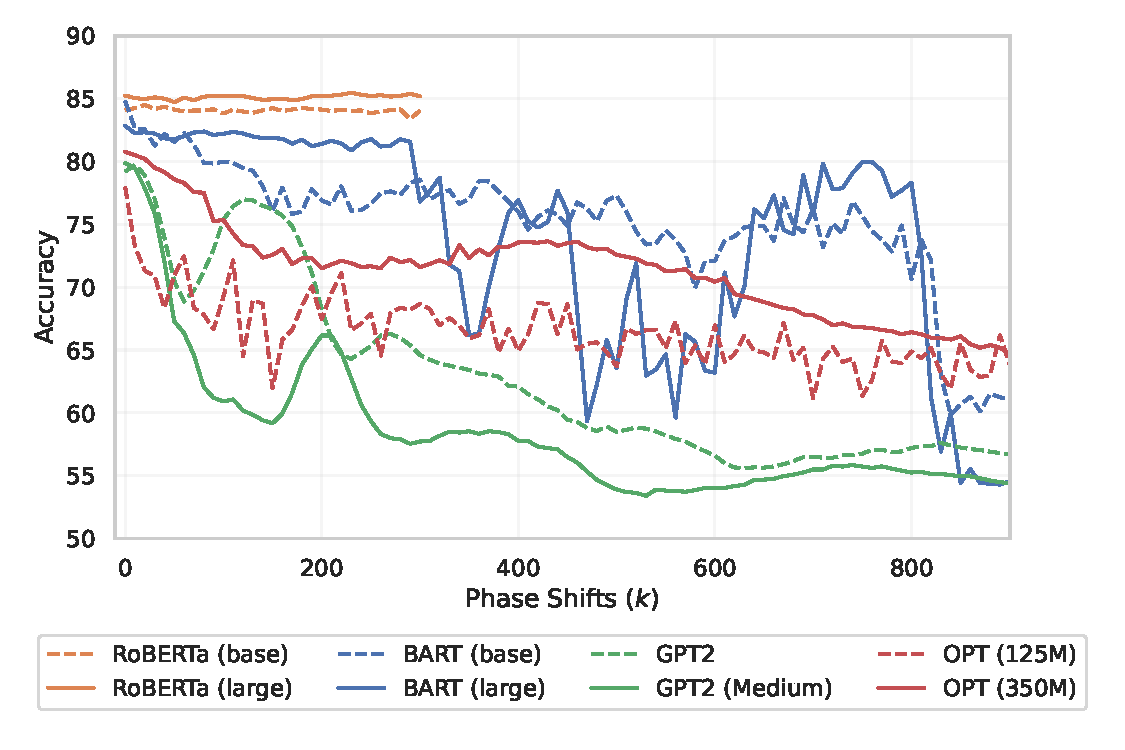
\includegraphics[width=\textwidth]{figs/pos/acceptability_scores.pdf}}
    \caption{Acceptability Scores in BLiMP \cite{warstadt-etal-2020-BLiMP-benchmark} dataset across different phase shifts. RoBERTa only supports context window of size $T=512$, so we capped the scores to phase shift $k=300$ to allow for sentences of maximum length in BLiMP to be evaluated.}
    \label{fig:acceptability}
\end{figure}


\begin{figure}
    \centering
    \resizebox{\linewidth}{!}{
    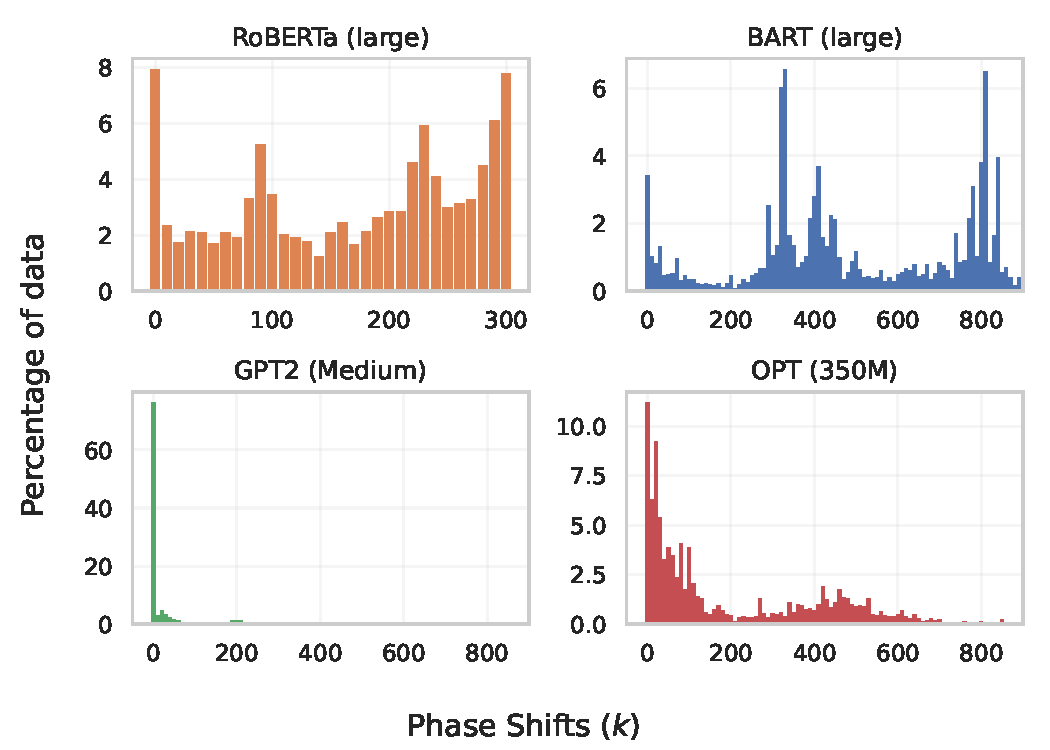
\includegraphics[width=\textwidth]{figs/pos/ppl_density_4.pdf}}
    \caption{Distribution of sentences in BLiMP \cite{warstadt-etal-2020-BLiMP-benchmark} having the lowest perplexities (i.e., are deemed most acceptable) for each phase shift.}
    \label{fig:ppl_density_main}
\end{figure}


First, we investigate the impact of phase shifting on the model performance.
We compute the perplexities of several publicly available models---RoBERTa \citep{liu-et-al-2019-roberta}, BART \citep{lewis-etal-2020-bart}, GPT2 \citep{Radford2019:GPT2} and OPT \citep{Zhang2022:OPT}---to evaluate the grammatical acceptability capabilities of the model, using the BLiMP \cite{warstadt-etal-2020-blimp} benchmark.\footnote{We adopt the perplexity computation strategy for RoBERTa and BART from \citet{salazar2020a}}
%Concretely, we measure the models' perplexity on grammatically correct and incorrect sentence pairs, and measure the accuracy on the model's ability to output a lower perplexity on the grammatical sentences.
We compute the task score by comparing grammatical and ungrammatical sentence perplexities, and applying the phase shift in increasing values of $k$ to the sentences and models (\autoref{fig:acceptability}).

While computing the task scores and perplexities of the models, we observed that all of the models exhibit poor task performance on phase shifts.
Due to the non-shiftable nature of the \texttt{[CLS]} token in masked language models (\acrshort{mlm}s), we fixed the position of \texttt{[CLS]} token to start position during phase shifting.
However, we observed a marked improvement in task performance when we use trigger tokens in the beginning of the sentence, typically the end-of-sentence (\texttt{[EOS]}) token in case of \acrshort{mlm} models (RoBERTa, BART).
An explanation for this ambiguity in results is that typically when models are pre-trained, multiple sentences are packed together in the context window by delimiting the start of each sentence with an \texttt{[EOS]} token.
While this is not the case for GPT2, we also observed improved performance in some cases when we add a beginning of sentence (\texttt{[BOS]}) token to the sentence and add a special \texttt{[EOS]} token to delimit the start of a sentence. Thus, in all of our results, we opt with this configuration (adding an \texttt{[EOS]} token before the sentence) to ensure fairer evaluation for all model families.
Concretely, the input to a model uses the following template:
$$
\texttt{[CLS]}\texttt{[EOS]} \texttt{<sentence>}
$$
In cases where a model does not have the \texttt{[CLS]} token, we instead use \texttt{[BOS]}.
If none of those are available, we replace it with \texttt{[EOS]} (so a total of two \texttt{[EOS]}'s will be prepended).
For phase shift $k$, we fix the position of \texttt{[CLS]} token to be the first available position in model's \acrshort{ape} (refer to \autoref{tab:model_detail}) and we shift every position id by $k$.
For example, given phase shift $k=100$, and first position id being 1, and sentence length of $n$, we have the following vector of position ids:
$$
\Vec{p} = [1, 100, 101, \dots, n+100]
$$


We observe that the task performance of all models, except for RoBERTa, drastically suffers from phase shifting. Autoregressive models in particular display worse results. This is likely due to a mismatch of position information learned due to the causal language modelling objective vs the position information provided to the model during phase shift \citep{haviv2022}. We also compare the perplexities of each sentence across different phase shifts and plot the frequency of sentences having the lowest perplexity in each $k$ (\autoref{fig:ppl_density_main}). We observe in GPT2 that more that 70\% of the sentences have their best perplexity in $k=0$, highlighting a severe zero-position bias. $\text{OPT}_{\text{350M}}$ has better sub-window sentence representation capacity than similarly sized GPT2, which is also evident from the acceptability results in \autoref{fig:acceptability}.


% As found by \citet{haviv2022}, autoregressive models trained on causal LM objective can operate optimally even without any positional information, due to a latent inductive bias.
% We conjecture that GPT2 performs worse as it is unable to reconcile with its internal position encodings vs the provided position encodings, similar to the findings by \citet{haviv2022}.
% Overall, majority of the tested models display a general bias towards the standard left-most position, which highlights the shortcomings of sub-window sentence representation.


% \section{Impact of position information on zero to few-shot settings}
\subsection{Impact of phase shifts on in-context learning}
\label{sec:pos_prompting_ps}

\begin{figure}
    \centering
    \resizebox{\linewidth}{!}{
    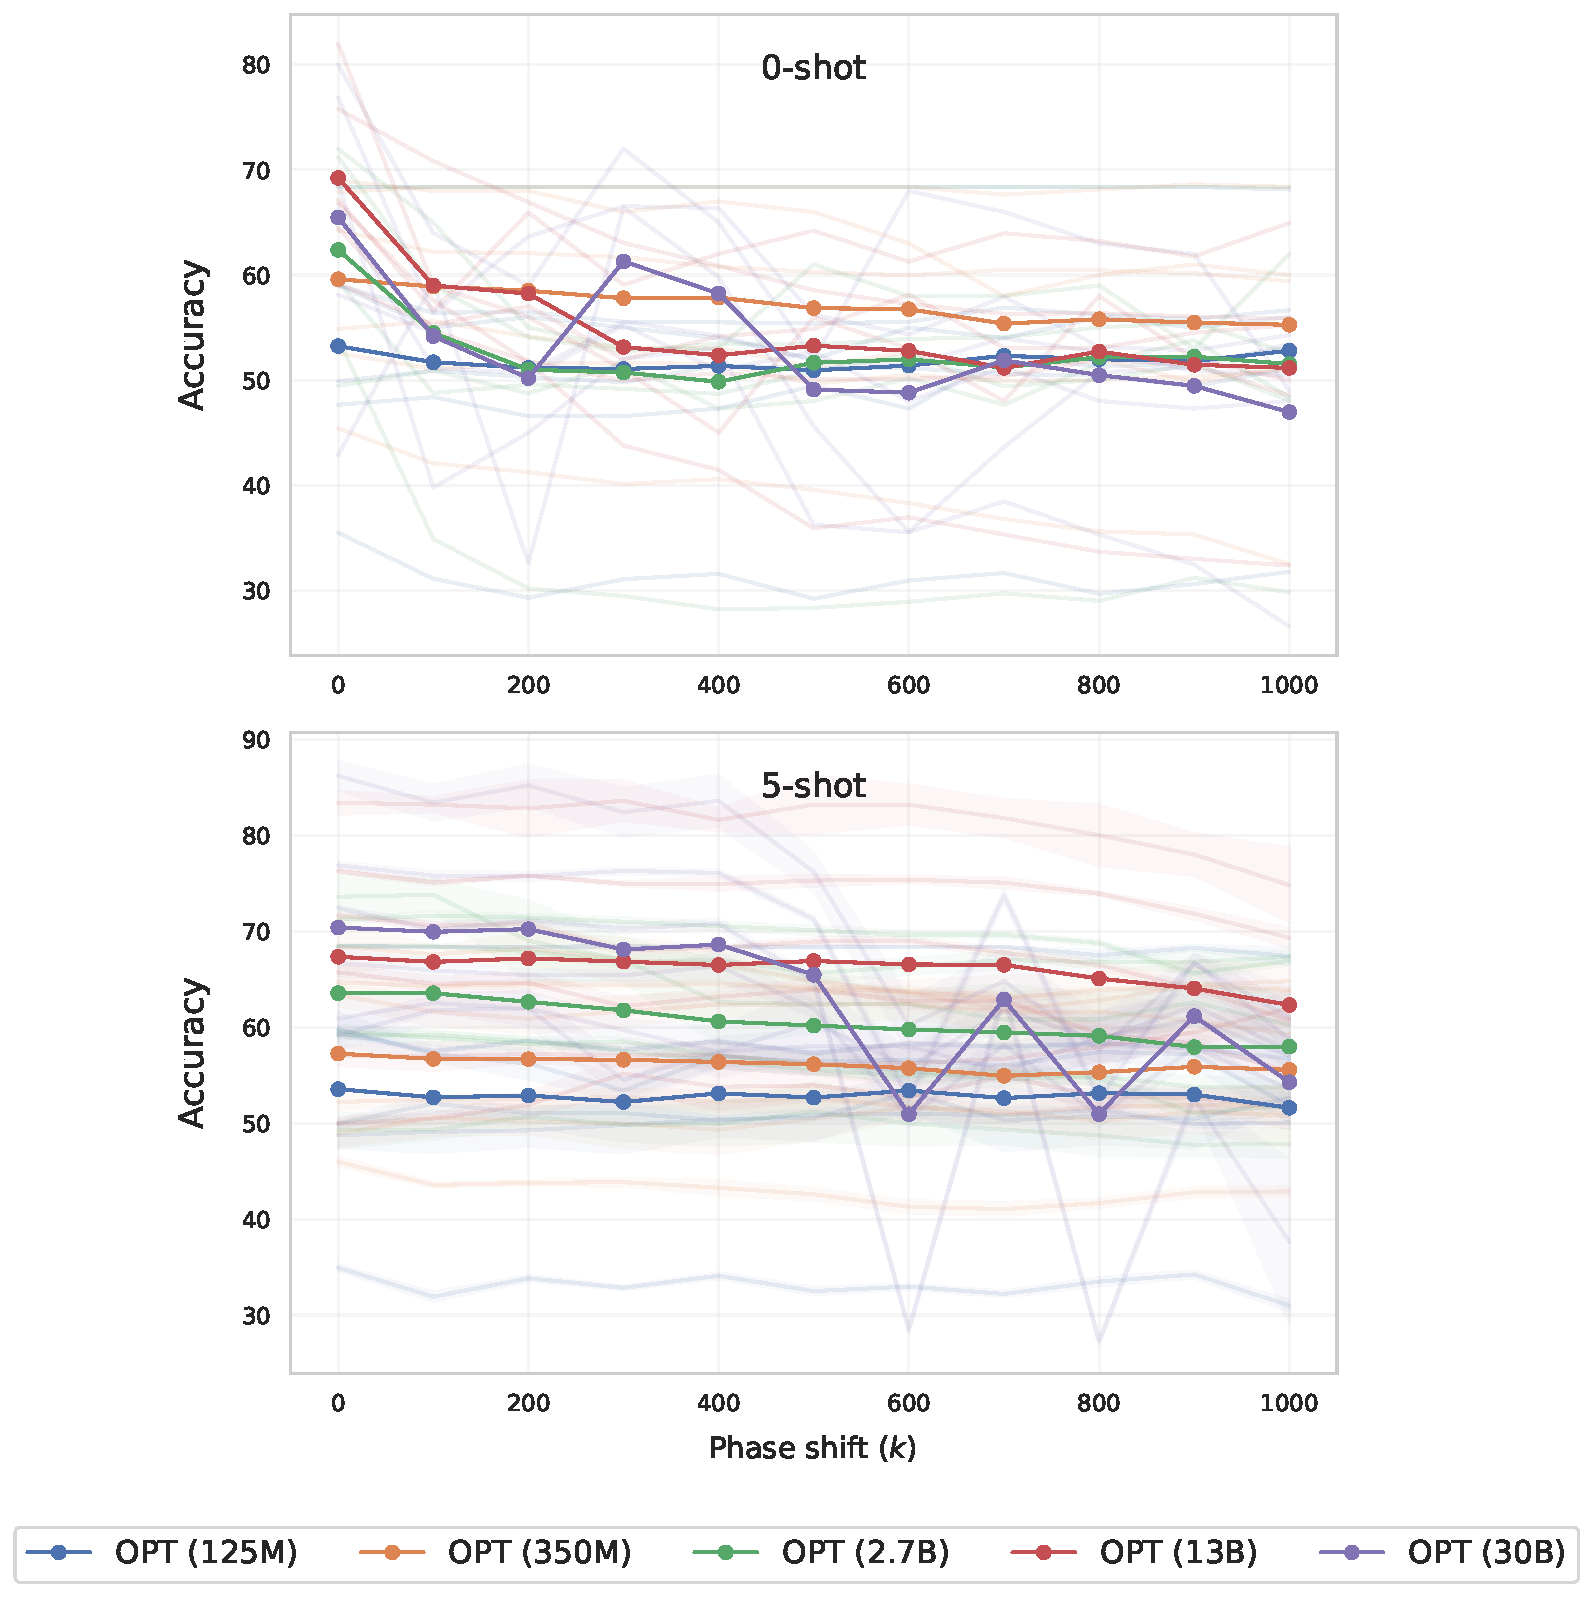
\includegraphics[width=0.9\textwidth]{figs/pos/v2_prompt_phase_shift_aggr_col.pdf}}
    \caption{Aggregate performance of OPT family on six NLP tasks when various phase shifts are applied.}
    \label{fig:prompt_ps_aggr}
\end{figure}


\begin{figure}
    \centering
    \resizebox{\linewidth}{!}{
    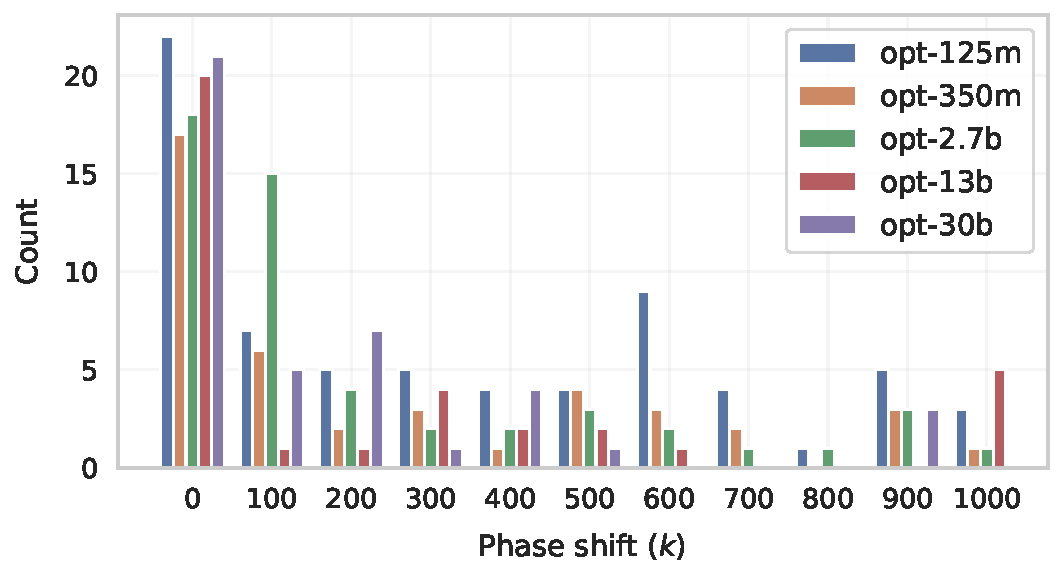
\includegraphics[]{figs/pos/v2_prompt_best_shifts (6).pdf}}
    \caption{Distribution of prompts with best accuracy across all six tasks.}
    \label{fig:prompt_best_ps}
\end{figure}


% in-context learning = recent technique large LM
% goal: measure its sensitivity to phase shift
% detail: follow EltherAI eval harness
% use tasks from OPT paper that had good performance
% scaling of the models
% result
% analysis
% - on avg. suffer
% - not always the case
% - scaling doest solve. bigger model perform is more harmed

% \begin{figure}
    \centering
    \resizebox{\linewidth}{!}{
    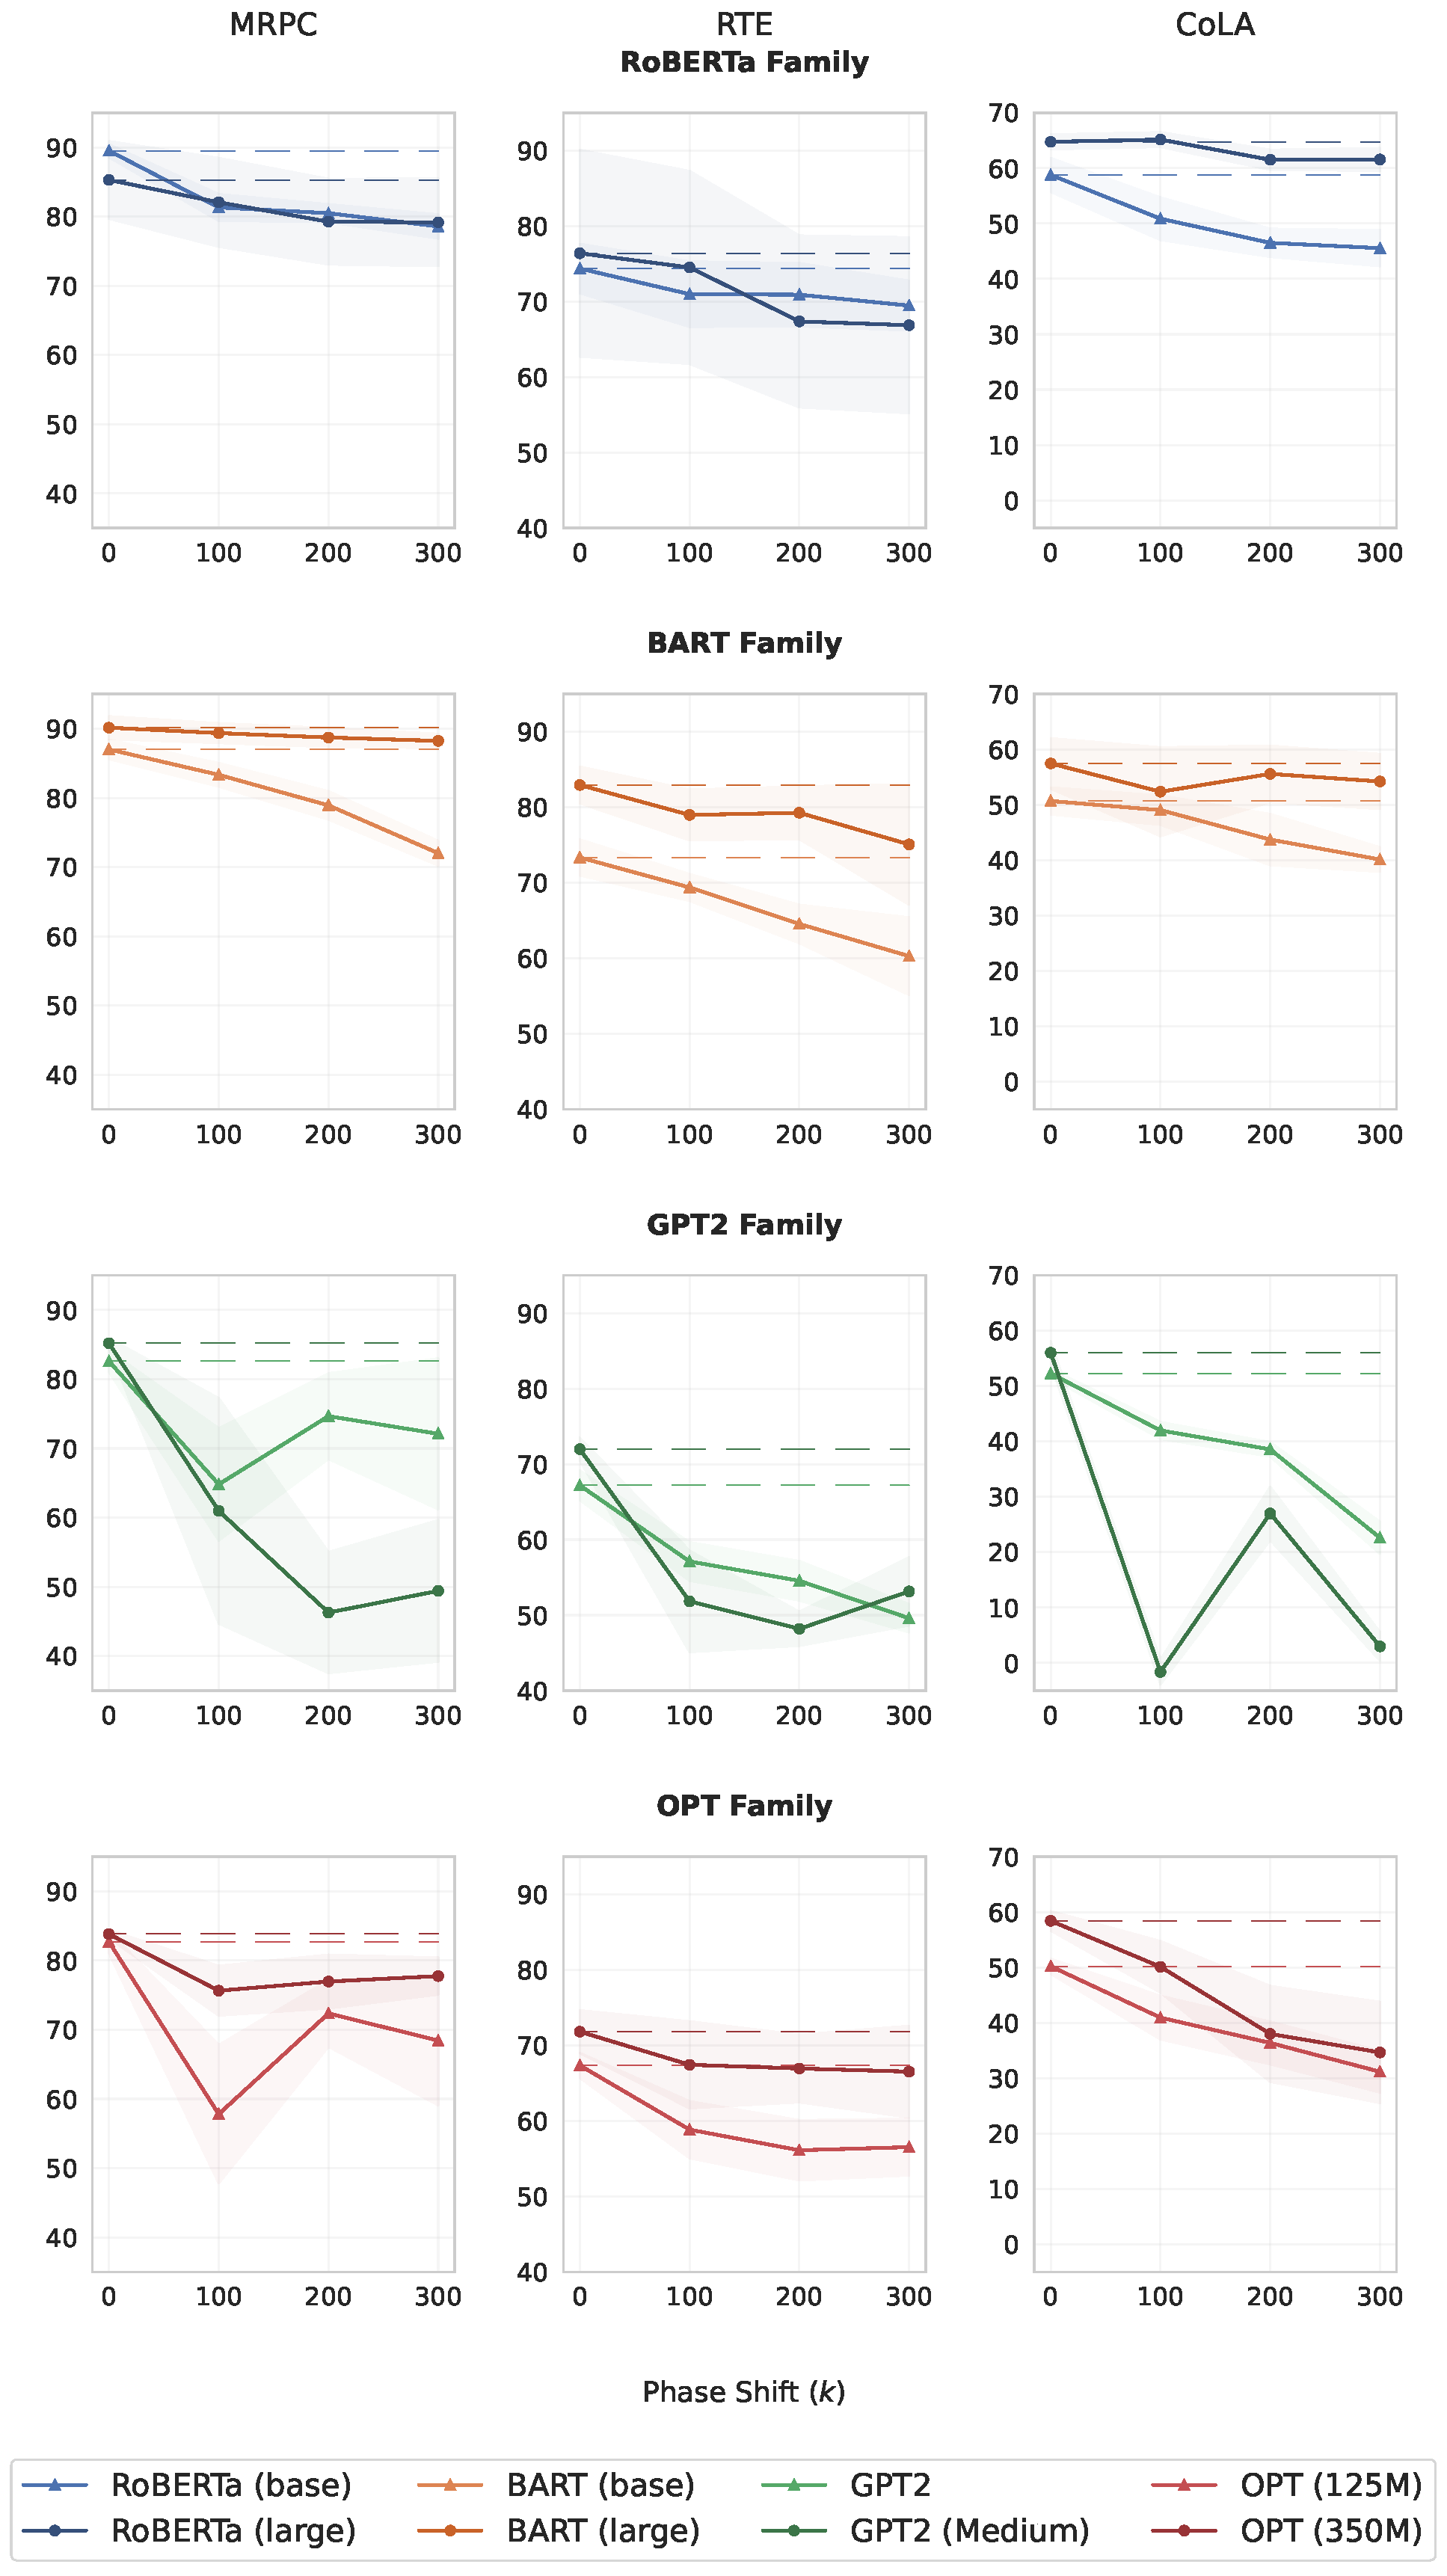
\includegraphics[width=\textwidth]{figs/glue_ps_0_eval_all_small.pdf}}
    \caption{GLUE downstream task results on CoLA, RTE and MRPC. The dashed lines represent the model performance with no phase shifts. The shaded area show the standard deviation from five random seeds.}
    \label{fig:glue_eval}
\end{figure}

More recently, zero-shot and few-shot inference, commonly referred to as in-context learning, have become a de facto standard in evaluating pretrained language models \citep{Brown2020:GPT3}.
In this approach, the model's predictions are produced by conditioning it on certain prompts, such as instructions (zero-shot setting) or a few examples of input-output pairs (few-shot setup).
In both cases, the model faces an extended input text, and we suspect it will be affected by deficiencies of \acrshort{ape}.
To evaluate this hypothesis, we employ an experimental setup similar to \autoref{sec:pos_acceptability}.
Under zero-shot and five-shot inference regimes, we assess the model performance on standard NLP tasks when it is fed with inputs in increasing values of phase shifts.
We choose OPT model family, because it is available in a wide range of sizes (125M to 30B parameters), allowing allows us to examine the behavior of \acrshort{ape} at different scales.
Moreover, our evaluations take into account four tasks reported in the original paper: Winogrande \citep{Sakaguchi2020:WINOGRANDE}, COPA \citep{Gordon2012:COPA}, PIQA \citep{Bisk2020:PIQA}, and ARC \citep{Clark2018:ARC} as well as two classification datasets from GLUE benchmark \citep{wang-etal-2018-glue}: MRPC and RTE.
%\footnote{In case of CoLA, we observed drastically worse result for prompting with OPT. Since it is an extreme outlier, we do not include it in \autoref{fig:prompt_ps_aggr}, but report it in Appendix.}
We provide an aggregated view of the models' performance on all six accuracy-dominated benchmarks in \autoref{fig:prompt_ps_aggr}. The detailed plots for each task are in \autoref{sec:pos_further_eval_prompts}.


%\paragraph{Unstable performance.}
% often the performance suffer
% periodic behaviour suggesting fitness to pre-training biases
% not always harms. Sometime improves.
In most tasks, the performance deteriorates when the model process inputs in any other phase shift than zero, especially in zero-shot inference.
More importantly, the model's performance is not always adversely affected by phase shifts. In fact, \autoref{fig:prompt_best_ps} shows that non-zero starting positions result in the best accuracy for many prompts.
% Although models tend to perform suboptimally with increasing $k$ values, the decline in accuracy is not entirely monotonic.
% Instead, models show periodic behavior pointing to a potential position bias that might exist in the pretraining data since some phase shifts seem to be a better match despite having larger values.
% Evaluating a model in a non-zero start position does not always harm the performance.
%For some combinations of tasks and models, the best accuracy can be obtained with $k$ > 0.
% For instance, OPT-30b achieves almost double the performance on zero-shot evaluation of MRPC when $k=300$ compared to zero phase shift. \autoref{fig:prompt_best_ps} shows many times non-zero start positions might are the best preferment ones.
%\paragraph{Scaling behaviour}
% erratic behaviour consistent in various model sizes
This erratic performance is present in all model sizes, and scaling the number of parameters does not help.
% pointing to data sparsity issue?
Furthermore, one can see larger models are more affected by shifted starting position, which suggests that absolute positional embedding might need more data or training as the number of parameters increases.

\subsection{Impact of phase-shifts on fine-tuning}
\label{sec:pos_finetuning}

Finally, we investigate the effect of phase shift in fine-tuning.
We ask whether the models can generalize to out-of-phase sentences for a given task.
We train RoBERTa, BART, GPT2 and OPT models on CoLA, RTE and MRPC tasks from the GLUE benchmark \citep{wang-etal-2018-glue} and evaluate them on phase-shifts.
We choose these three relatively small tasks in order to decrease the number of gradient updates to position embeddings during fine-tuning.
We perform a cross-phase analysis by training and evaluating across different phase shifts ($k={0,100,200,300})$ for all models on the same set of datasets, and show the averaged performance.
We observe for all models, the task performance drops during out-of-phase evaluation (non-diagonals in \autoref{fig:glue_phaseshift}).
% This drop is more accentuated for BART, which is in-line with our grammatical acceptability results.

\begin{figure}
    \centering
    \resizebox{\linewidth}{!}{
    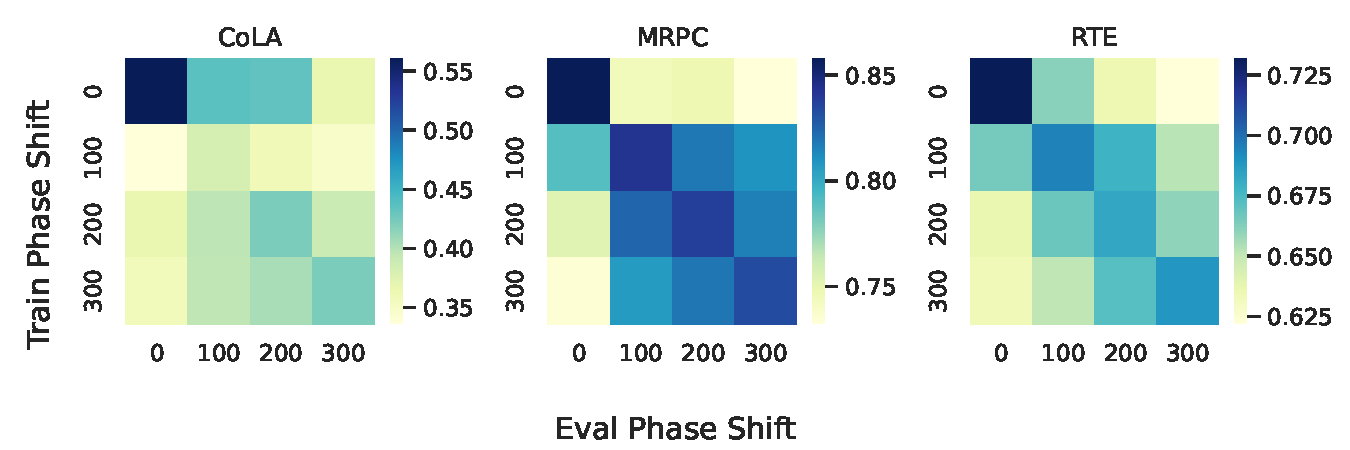
\includegraphics[width=\textwidth]{figs/pos/phase_shift_heatmap.pdf}}
    \caption{GLUE task heatmap with varying fine-tuning train and test phase shifts, averaged across all models. Darker colors represent better task performance.}
    \label{fig:glue_phaseshift}
\end{figure}


The drop in performance of evaluating out-of-phase sentences might just be simply attributed to overfitting on position information during fine-tuning.
% Thus, we further ask the question on whether fine-tuning on different phase-shifted sentences also yield similar performance as in fine-tuning on the standard, zero position.
However, we observe that for all tasks, training and evaluating on the same phase-shift is worse when $k \ne 0$ (diagonals in \autoref{fig:glue_phaseshift}).
Out-of-phase training appears to be worst for CoLA, which suffers drastically when fine-tuning on different phase shifts.
These results highlight a potential task data bias with respect to different positions.



\section{Analysis}
\label{sec:pos_analysis}

\subsection{Further evaluation on Phase shifting with prompts}
\label{sec:pos_further_eval_prompts}

We displayed a holistic view of zero-shot and five-shot experiments in \autoref{fig:prompt_ps_aggr}, covering the accuracies averaged over all six datasets.
%However, it should not be taken as an accurate measure or benchmark.
In this section, we now report and analyze the result of each dataset individually. \autoref{fig:propmt_all_ds_part0} and \autoref{fig:propmt_all_ds_part1} showcase models' performance in zero-shot and five-shot configurations.
The same pattern can be seen across all model sizes in COPA, WinoGrande, PIQA, ARC (Easy), and RTE. Concretely, the zero-shot abilities of the models sharply decrease as we increase the starting position.
Moreover, five-shot inference, typically referred to as in-context learning, is also subject to decreased performance, ranging from -2\% to -40\%. However, the degradation is not as severe as with zero-shot setting.
Only MRPC exhibits stable phase shift performance, but even in this case, larger models are still adversely affected. Due to the exceptionally poor performance of OPT family on CoLA, we exclude these results from our analysis (\autoref{fig:propmt_all_ds_part1}).

\begin{figure*}
    \centering
    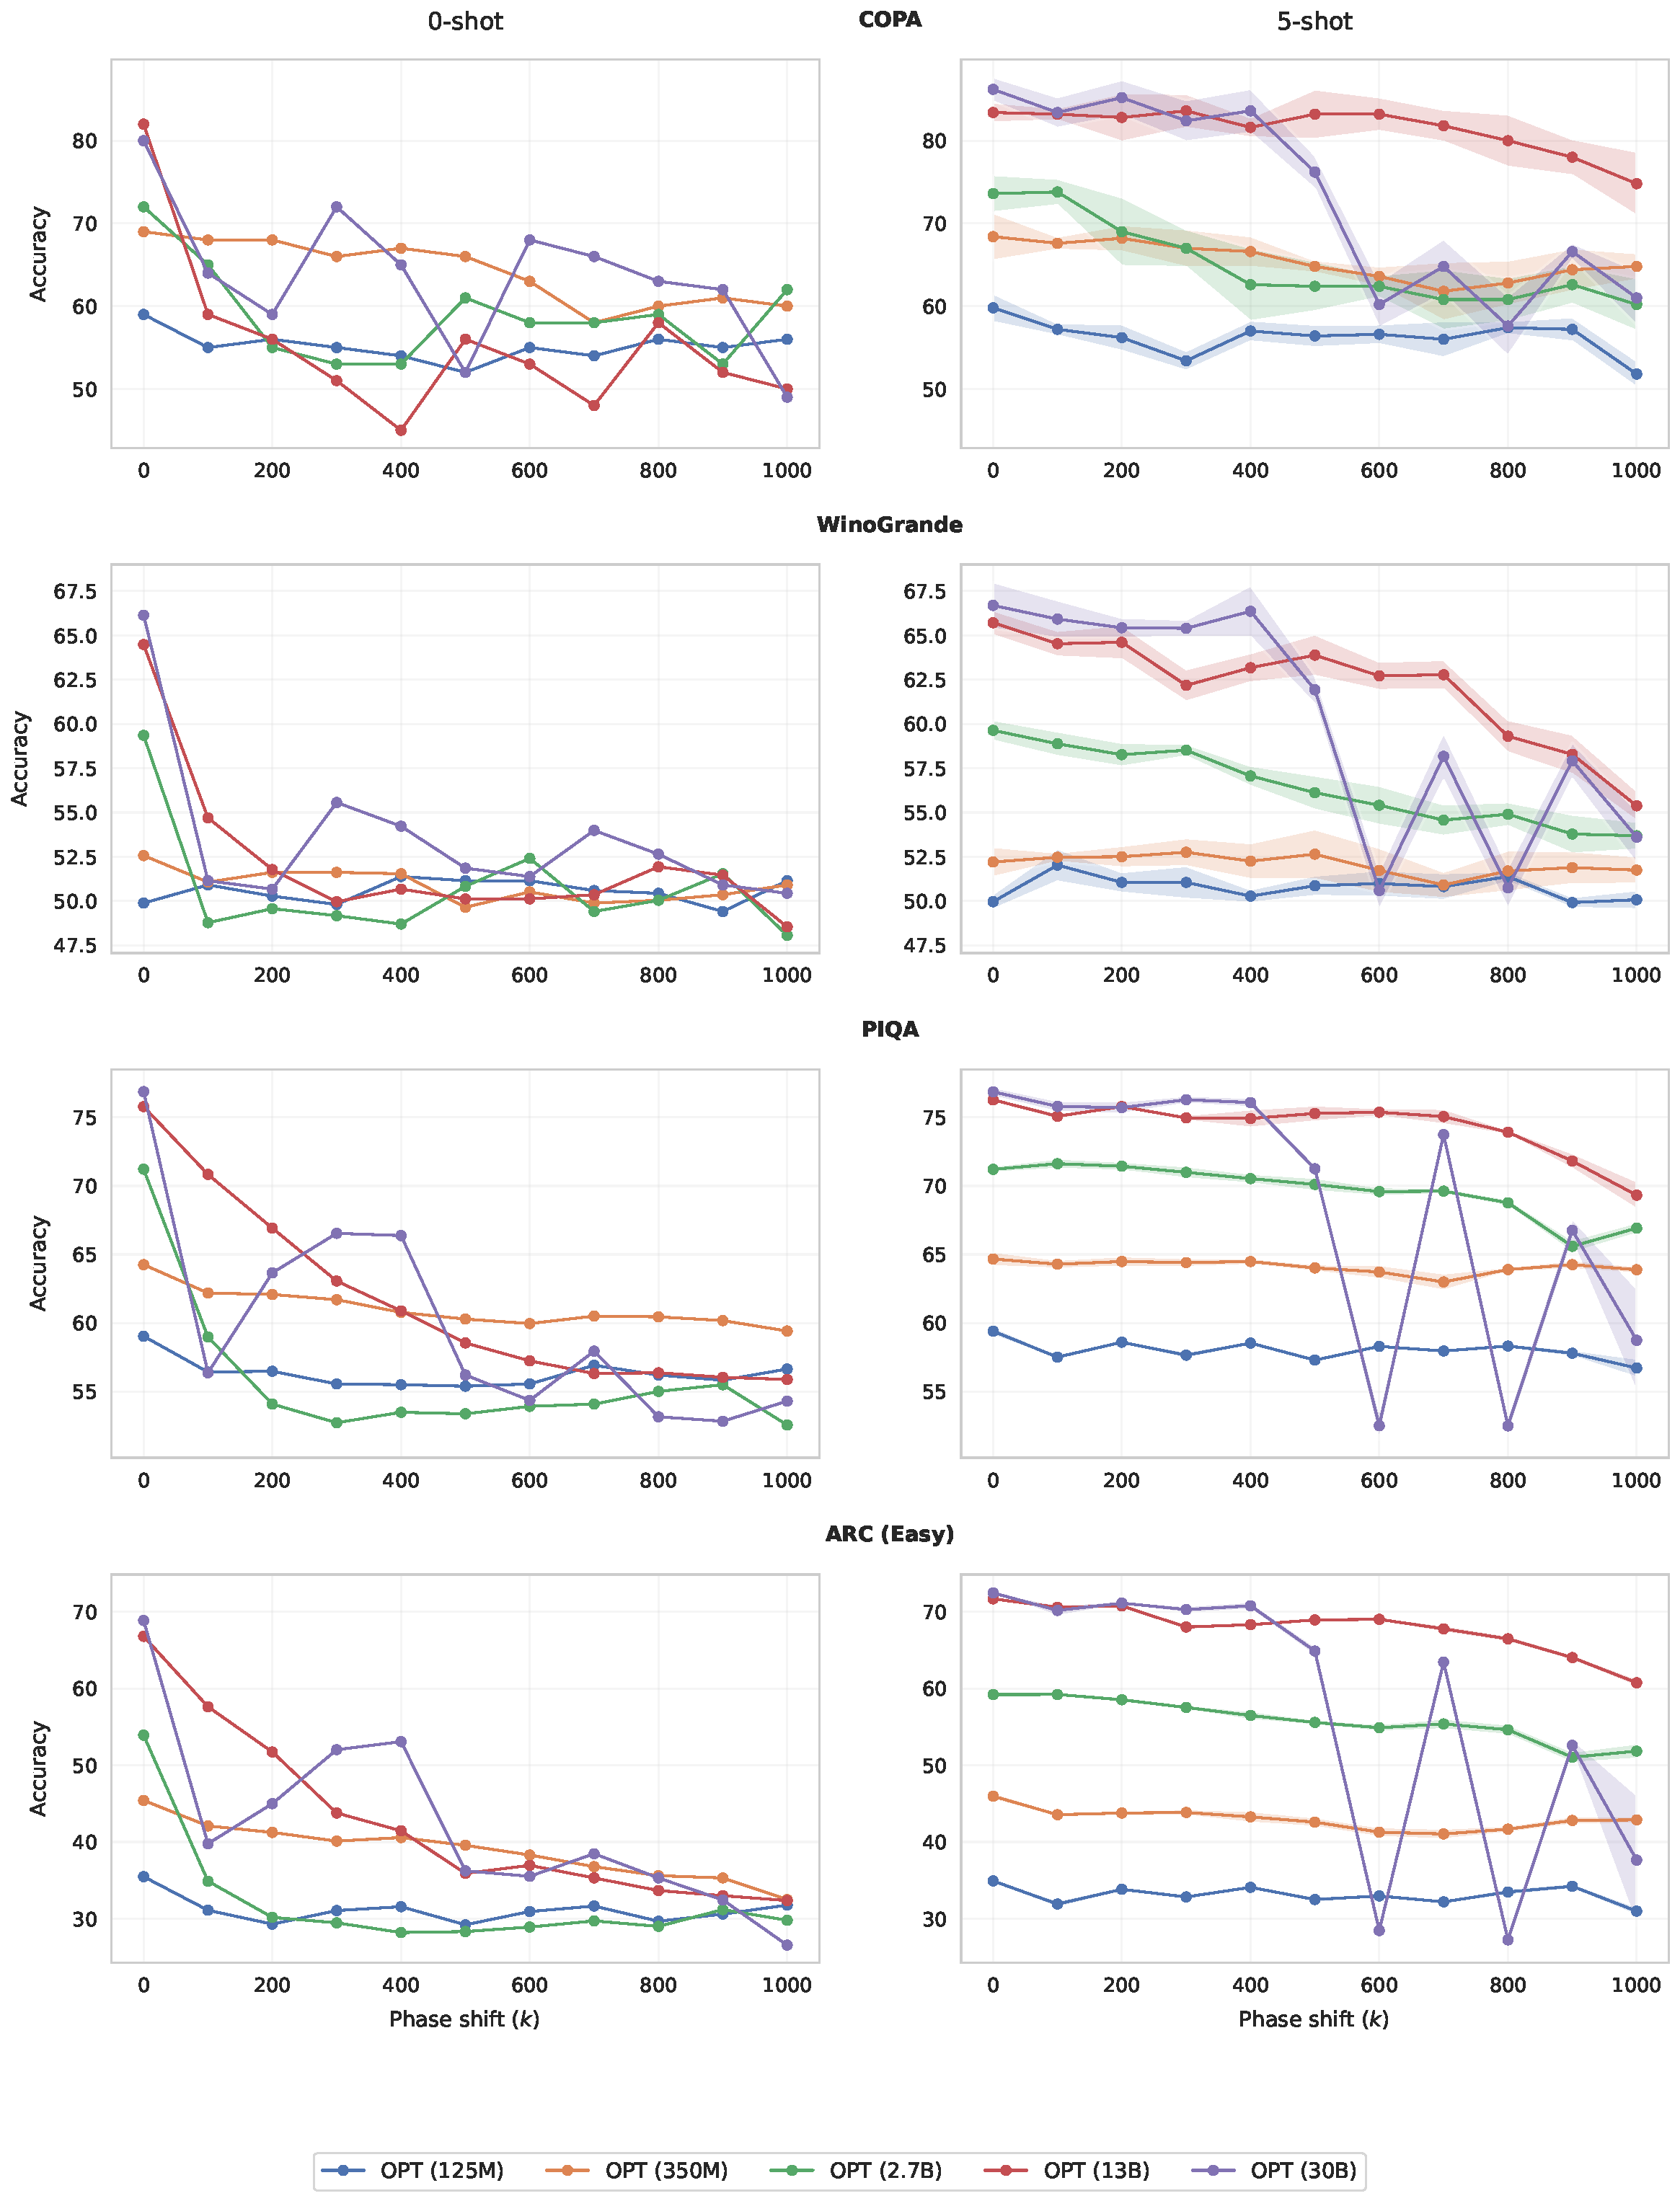
\includegraphics[width=\textwidth]{figs/pos/v2_prompt_phase_shift_all_ds_part0.pdf}
    \caption{Zero-shot and Few-shot performance of OPT family with various phase shifts for each individual dataset (Part 1)}
    \label{fig:propmt_all_ds_part0}
\end{figure*}

\begin{figure*}
    \centering
    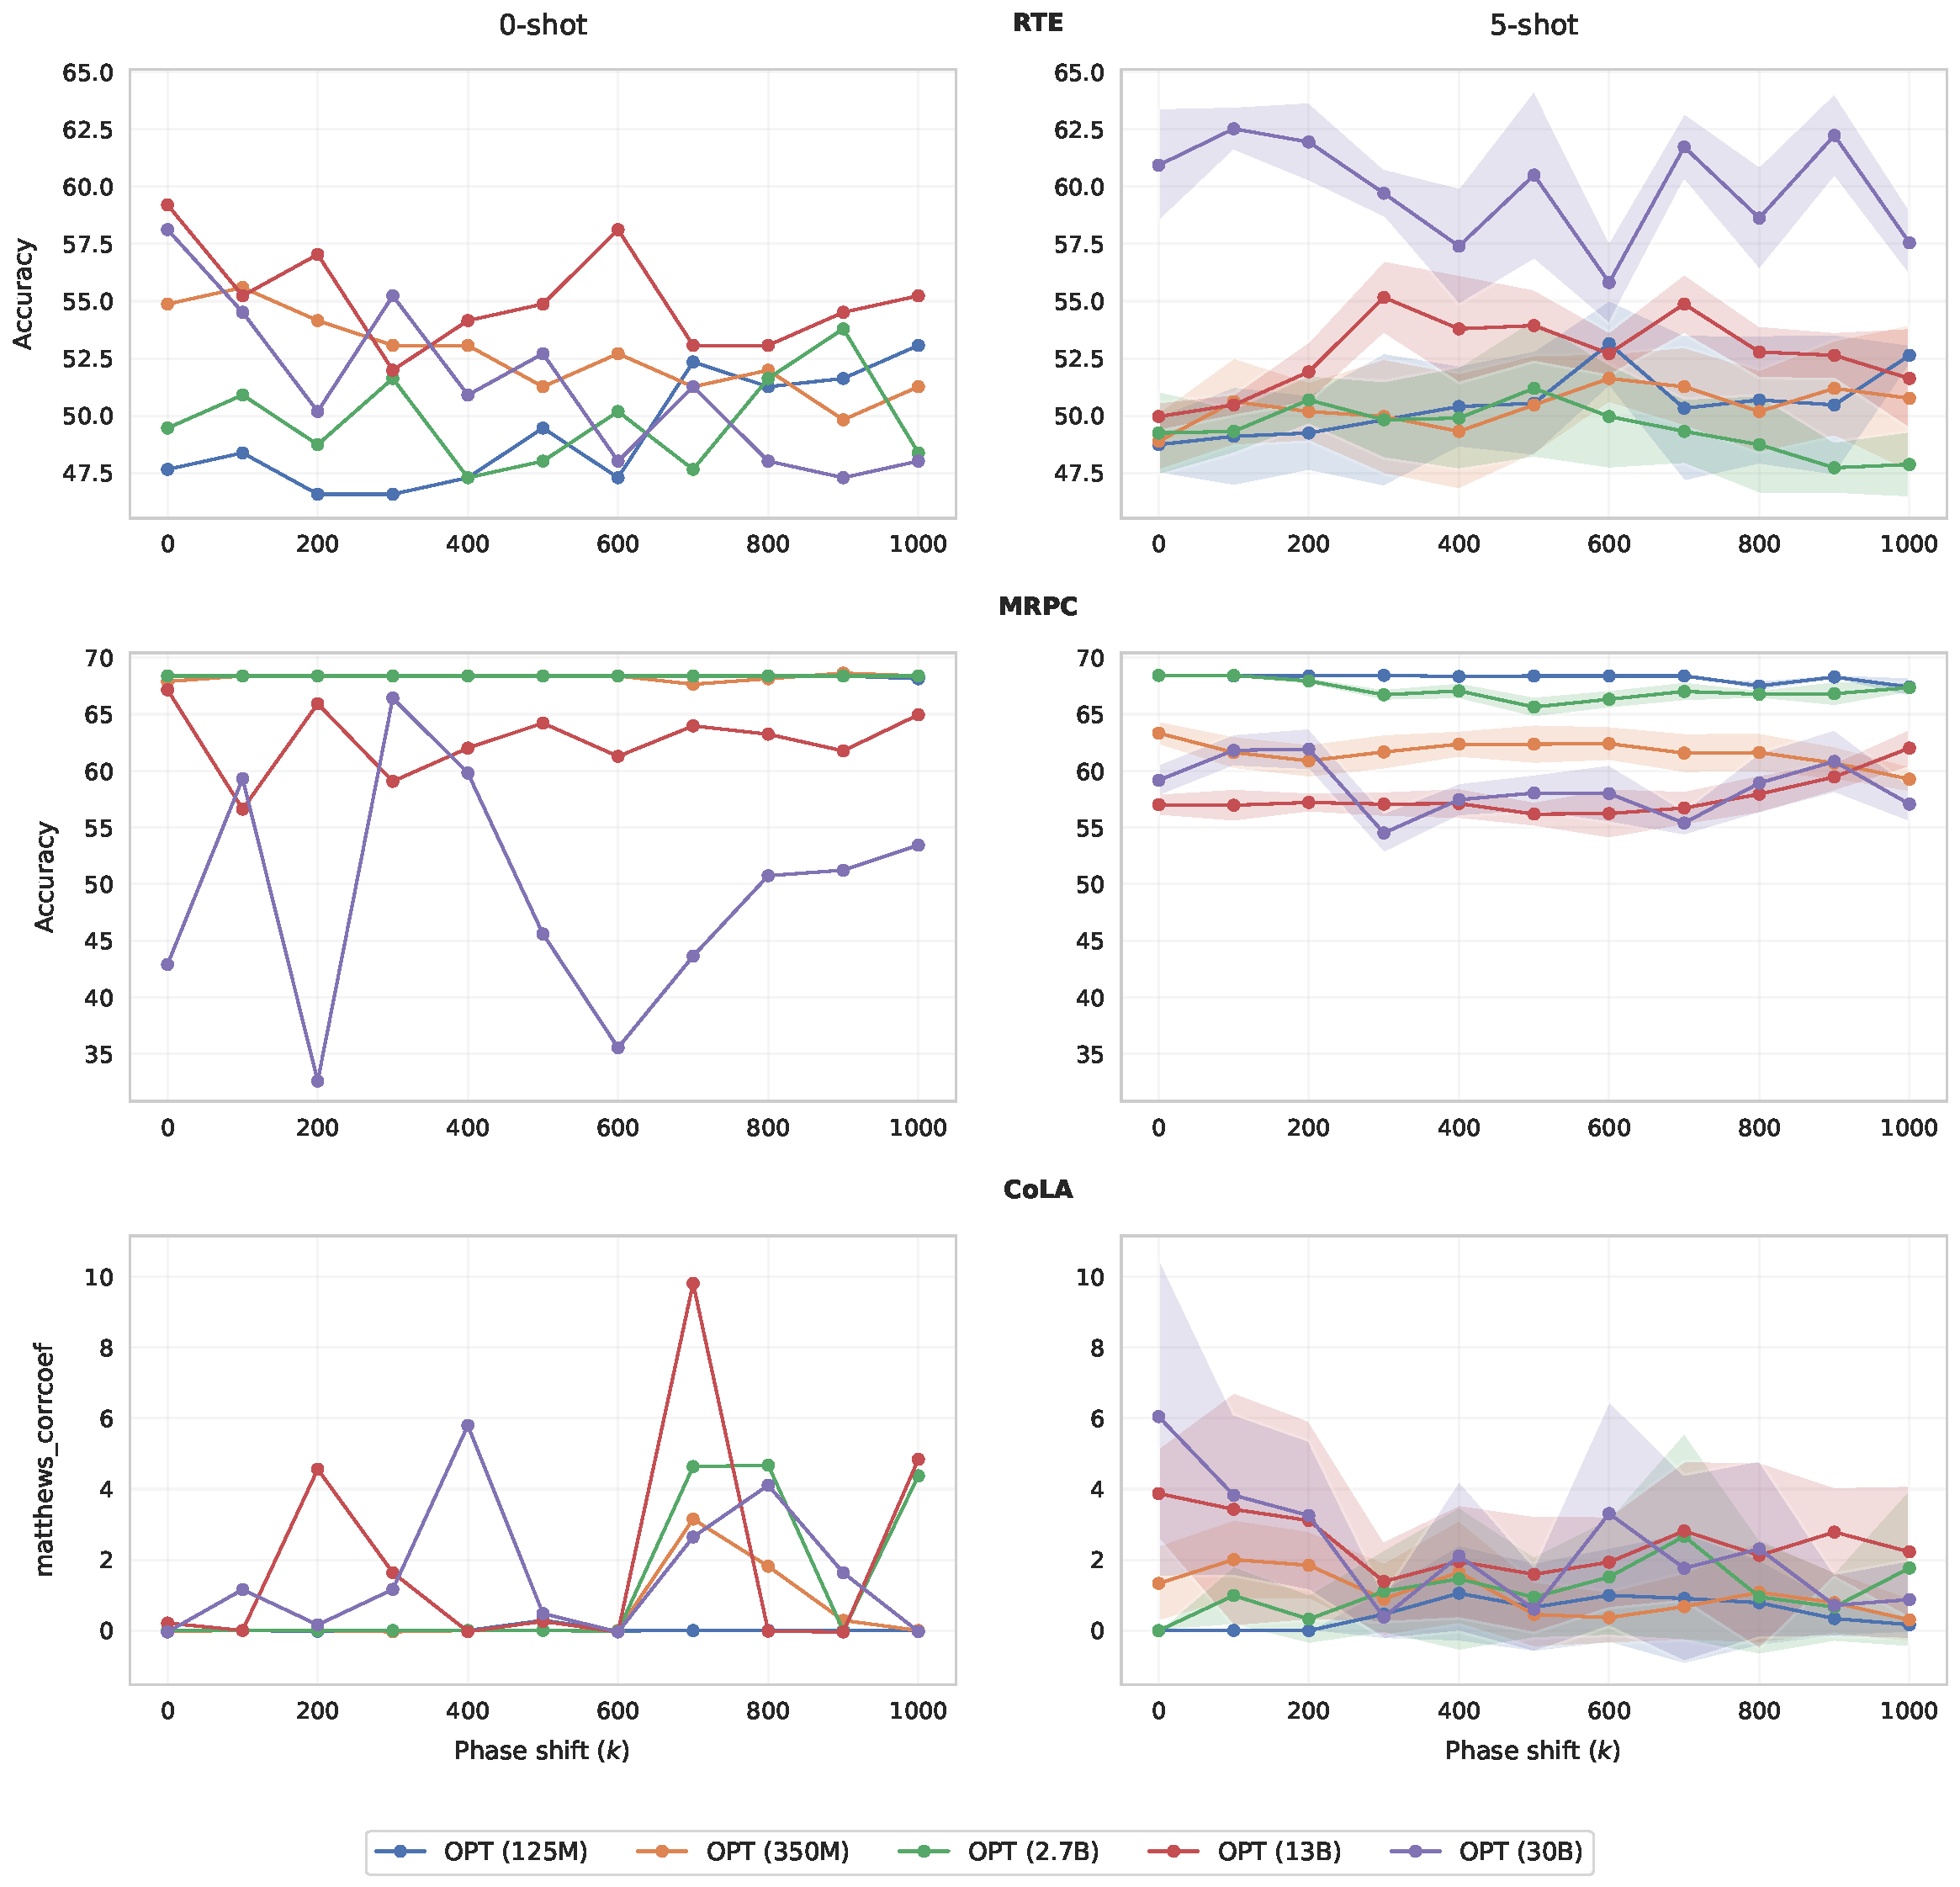
\includegraphics[width=\textwidth]{figs/pos/v2_prompt_phase_shift_all_ds_part1.pdf}
    \caption{Zero-shot and Few-shot performance of OPT family with various phase shifts for each individual dataset (Part 2)}
    \label{fig:propmt_all_ds_part1}
\end{figure*}



The erratic behaviour observed in majority of evaluated datasets makes it evident that models struggle to encode the relative distances of words as their understanding of inputs heavily change with various phase shifts.
It is important to note that our findings demonstrate models' unstable functioning as opposed to solely highlighting their failure. Indeed, \autoref{fig:prompt_best_ps} shows that one can extract better and improved accuracies with non-zero starting positions.
Namely, $\text{OPT}_{\text{30B}}$ has the best zero-shot performance on phase shift $k=300$ in the case of MRPC; the same pattern can also be observed in RTE five-shot for $\text{OPT}_{\text{13B}}$ on phase shift $k=300$.
Another noteworthy observation is that the performance drop is often a \emph{non-monotonic} function of phase shifts. i.e., for some prompts, the model might be more accurate for $k=1000$ than for $k=0$.
This observation suggests that some positional biases might be learned during pre-training and are well-captured by \acrshort{ape}. So, increasing values of $k$ in some occasions lands the model attentions in a ``sweet spot'' in the processing window, such that the model benefits from some positional biases learned during pre-training.

We observe the presence of erratic behavior across a fairly wide range of model sizes in the OPT family. Additionally, it can be seen that larger models are more prone to fail at encoding relative positions than their smaller counterparts.
One possible explanation for this is that in order for the models to encode relative positional information, they need to view all combinations of words and sentences in every position. This coverage rarely occurs in natural data, resulting in data sparsity issues. Hence, models with a large number of parameters may require more data/training to learn the relative ordering of words.

\subsection{Variation of best perplexity across phase shifts}
\label{sec:pos_perplexity_phase}

\begin{figure}[!ht]
    \centering
    \resizebox{0.8\linewidth}{!}{
    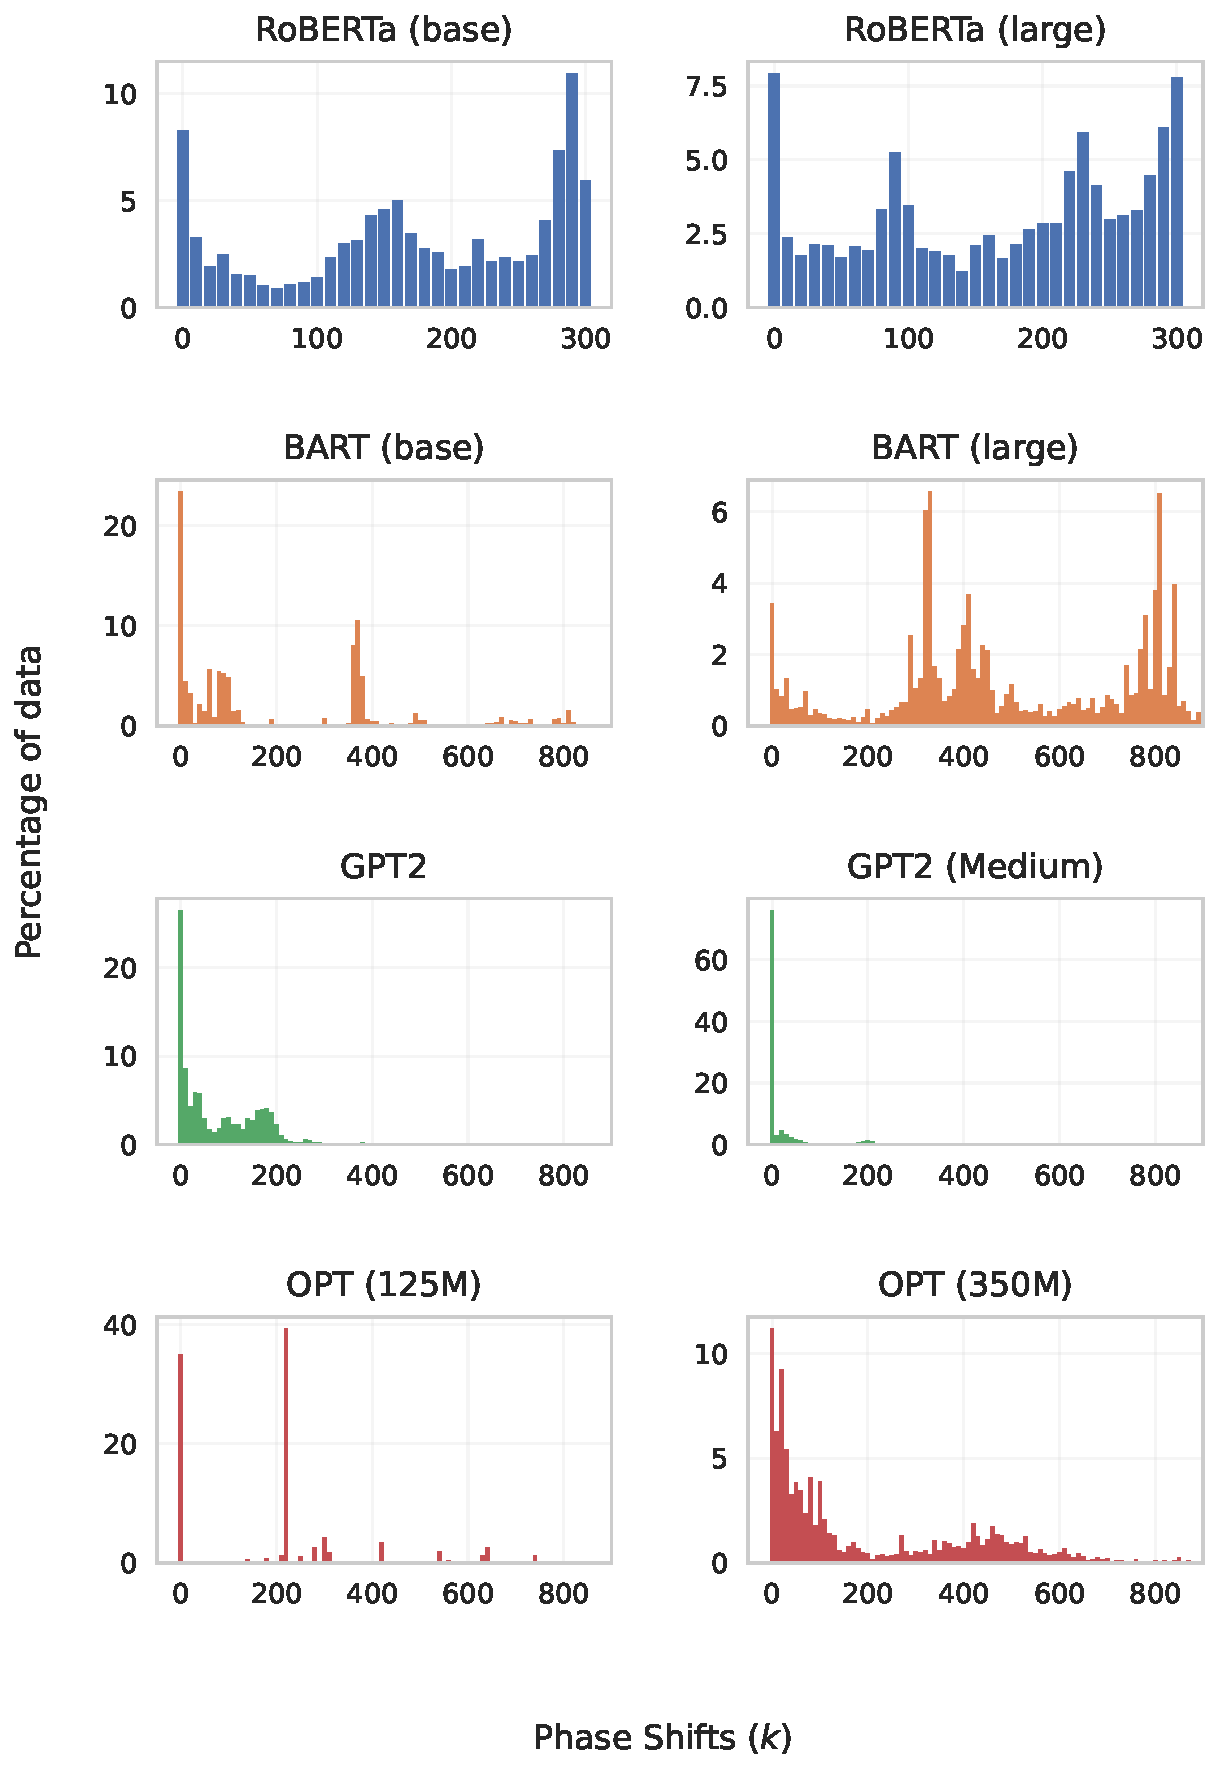
\includegraphics[]{figs/pos/ppl_density_all.pdf}}
    \caption{Distribution of sentences having the lowest perplexities for each phase shift}
    \label{fig:ppl_density}
\end{figure}

In this section, we investigate the perplexity of individual sentences from the BLiMP dataset across each phase shift for each model. We plot the distribution of sentences achieving lowest perplexity in each phase shift for the range of models in \autoref{fig:ppl_density}. We observe several modes of phase shift for RoBERTa and BART models where they have the least perplexity on phase shifts other than the standard (zero position). In the case of GPT2 and OPT, the distribution is more skewed towards zero, indicating they almost always achieve the lowest perplexity in the zero position, i.e. when there is no phase shift.

\subsection{Variation in attention patterns with phase shift}
\label{sec:pos_attention_analysis}


We further perform attention analysis on GPT2, RoBERTa and BART to visualize whether the model's attention pattern changes with phase shifts. Following the experimental protocol of \citet{raghu2021vision}, we first collect a summary of attention weights computed with token distances for each token-pair in a sentence. This summary metric is then further normalized for sentence length. The values of this metric show whether the attention is local (low values)---focused on small token distances---or global (high values)---i.e. focused on the whole sentence.

We compute this attention summary metric on a sample of 5000 sentences drawn from the BLiMP dataset \cite{warstadt-etal-2020-blimp}. We then plot the summary values per layer and sort according to the values for each attention head, as per \citet{raghu2021vision}. The idea is to discover whether this attention summary metric is drastically different under different phase shift conditions. %This analysis further highlights the importance of studying the relativity of \acrshort{ape}s closely.

We do observe drastic differences in attention patterns in all layers for GPT2 (\autoref{fig:globality_GPT2}) and GPT2-Medium (\autoref{fig:globality_GPT2-medium}). Comparing this with of RoBERTa (base) (\autoref{fig:globality_roberta-base}) and RoBERTa (large) (\autoref{fig:globality_roberta-large}), we can corroborate our findings from \autoref{sec:pos_acceptability}---RoBERTa is much more robust to phase shifts. Consequently, BART (\autoref{fig:globality_bart-base} and \autoref{fig:globality_bart-large}) also displays differences in attention patterns, but they are not as drastic as GPT2.

\begin{figure*}
    \centering
    \resizebox{0.8\linewidth}{!}{
    \includegraphics[]{figs/pos/locality_GPT2_sentence_good.pdf}}
    \caption{Attention globality distributions of GPT2 across different heads (sorted according to value) and averaged over all layers and 5000 data points. Blue curve stands for the no phase shift condition, and orange, green and red curves represent $k=100,200$ and $300$ respectively.}
    \label{fig:globality_GPT2}
\end{figure*}

\begin{figure*}
    \centering
    \resizebox{0.7\linewidth}{!}{
    \includegraphics[]{figs/pos/locality_GPT2-medium_sentence_good.pdf}}
    \caption{Attention globality distributions of GPT2-Medium across different heads (sorted according to value) and averaged over all layers and 5000 data points. Blue curve stands for the no phase shift condition, and orange, green and red curves represent $k=100,200$ and $300$ respectively.}
    \label{fig:globality_GPT2-medium}
\end{figure*}

\begin{figure*}
    \centering
    \resizebox{\linewidth}{!}{
    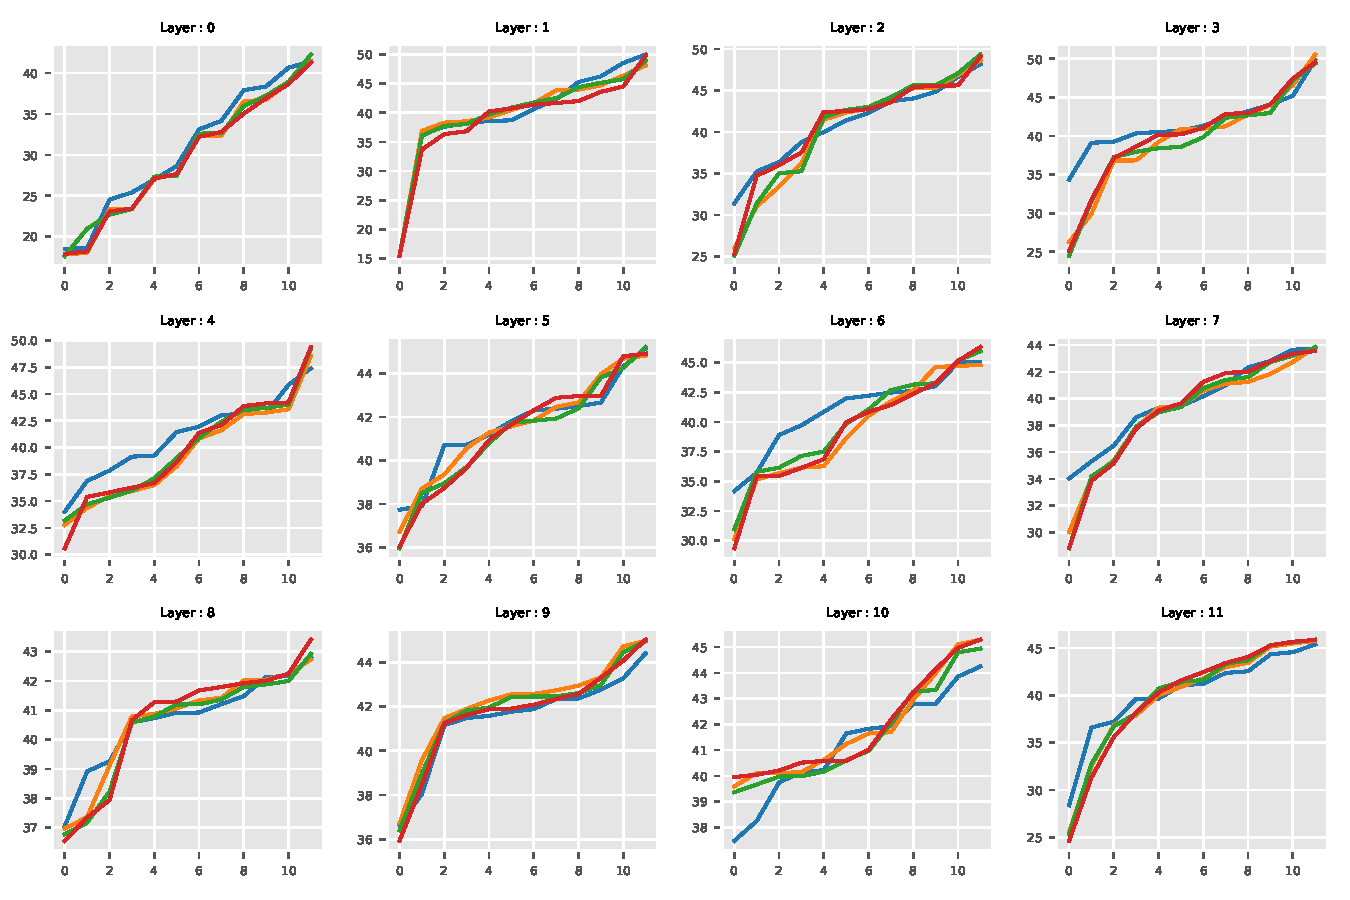
\includegraphics[width=\textwidth]{figs/pos/locality_roberta-base_sentence_good.pdf}}
    \caption{Attention globality distributions of RoBERTa (base) across different heads (sorted according to value) and averaged over all layers and 5000 data points. Blue curve stands for the no phase shift condition, and orange, green and red curves represent $k=100,200$ and $300$ respectively.}
    \label{fig:globality_roberta-base}
\end{figure*}

\begin{figure*}
    \centering
    \resizebox{0.7\linewidth}{!}{
    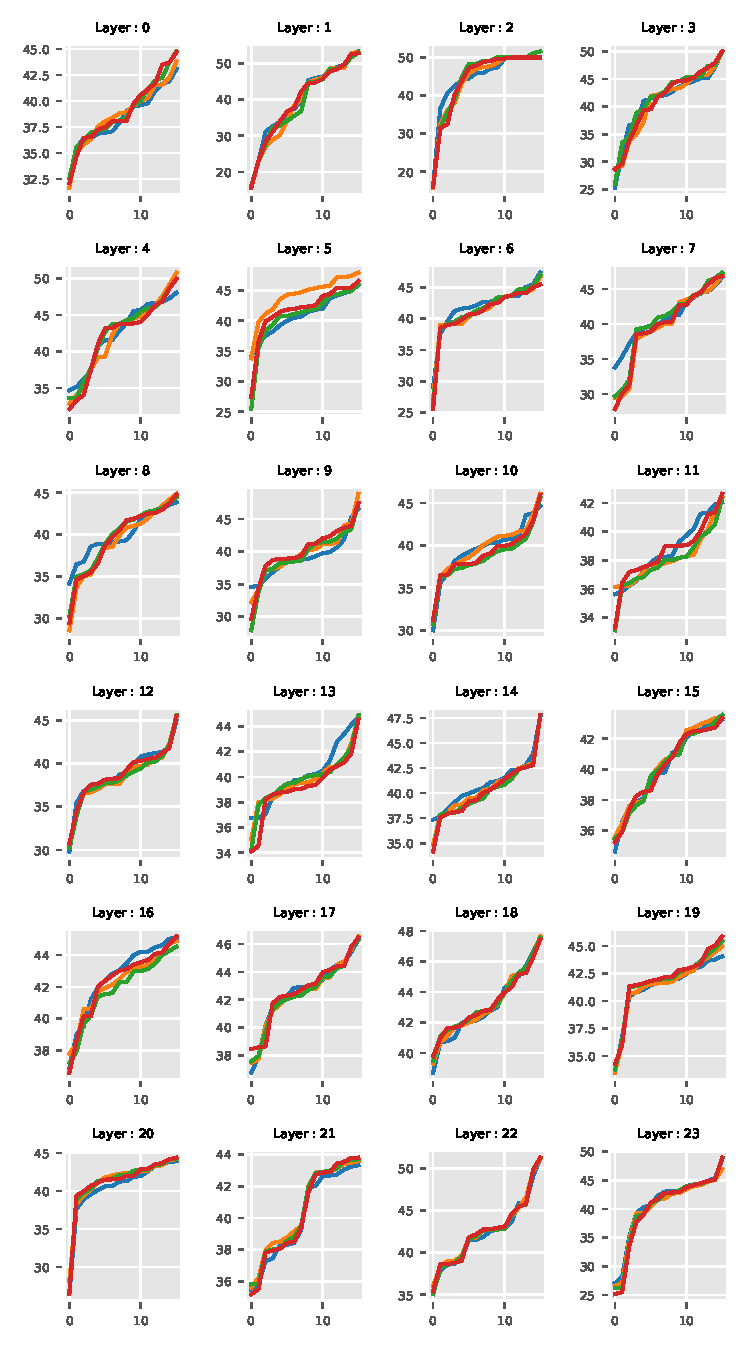
\includegraphics[]{figs/pos/locality_roberta-large_sentence_good.pdf}}
    \caption{Attention globality distributions of RoBERTa (large) across different heads (sorted according to value) and averaged over all layers and 5000 data points. Blue curve stands for the no phase shift condition, and orange, green and red curves represent $k=100,200$ and $300$ respectively.}
    \label{fig:globality_roberta-large}
\end{figure*}

\begin{figure*}
    \centering
    \resizebox{\linewidth}{!}{
    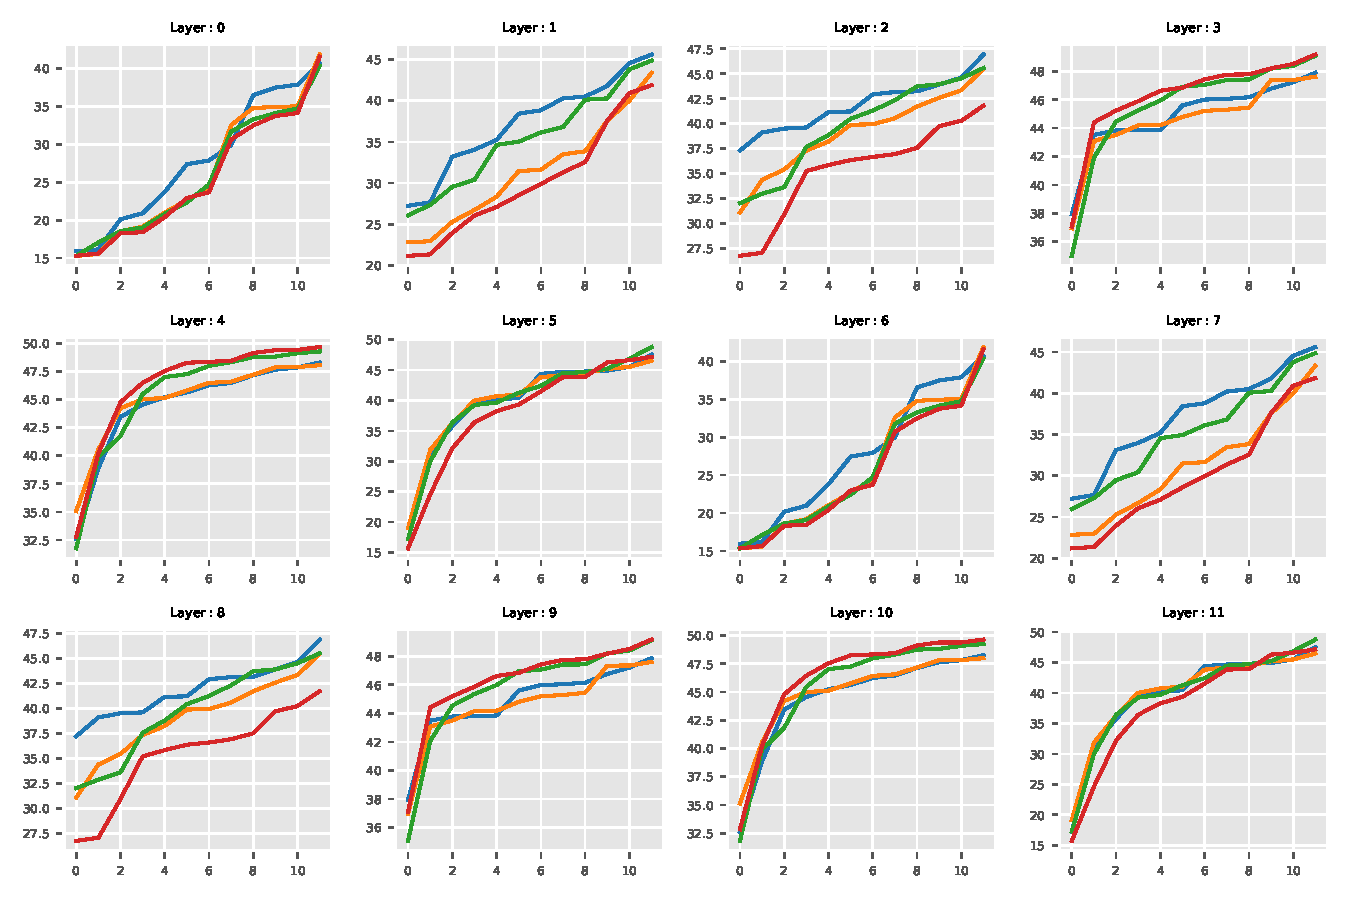
\includegraphics[width=\textwidth]{figs/pos/locality_facebook-bart-base_dec_sentence_good.pdf}}
    \caption{Attention globality distributions of BART (base) across different heads (sorted according to value) and averaged over all layers and 5000 data points. Blue curve stands for the no phase shift condition, and orange, green and red curves represent $k=100,200$ and $300$ respectively.}
    \label{fig:globality_bart-base}
\end{figure*}

\begin{figure*}
    \centering
    \resizebox{0.8\linewidth}{!}{
    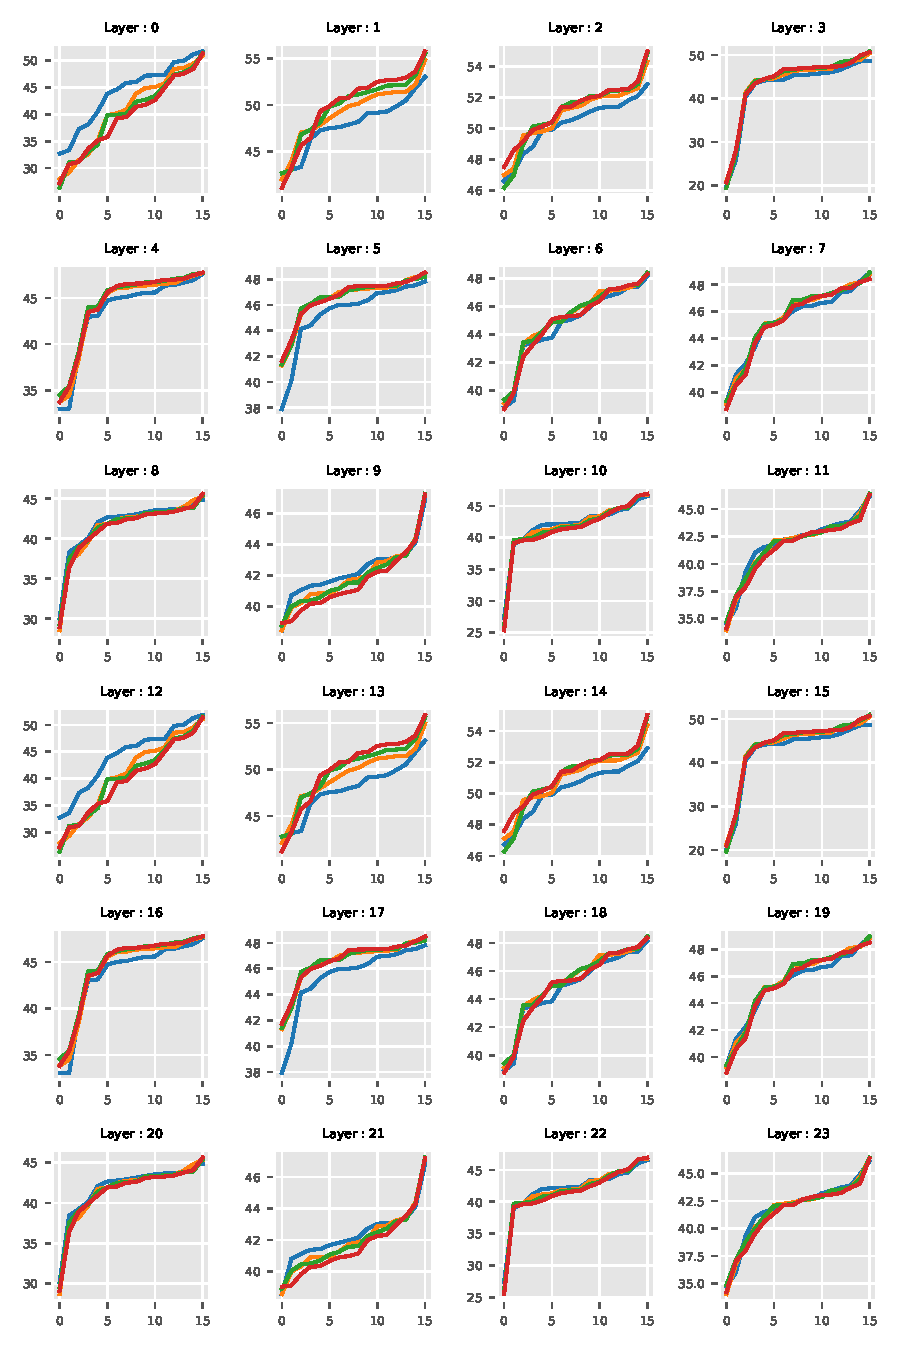
\includegraphics[]{figs/pos/locality_facebook-bart-large_dec_sentence_good.pdf}}
    \caption{Attention globality distributions of BART (large) across different heads (sorted according to value) and averaged over all layers and 5000 data points. Blue curve stands for the no phase shift condition, and orange, green and red curves represent $k=100,200$ and $300$ respectively.}
    \label{fig:globality_bart-large}
\end{figure*}



\section{Related Work}
\label{sec:pos_related_work}

Positional encoding has been always an important part of the Transformer architecture, and since it original introduction different variants of it have been deployed by pretrained models (see \autoref{tab:models_pe} for a summary of positional encoding used by some of popular state-of-the-art models.)
% Positional embeddings have been something of a cottage industry in NLP, enabling several works exploring the inner workings of the Transformer-class of models.

Positional encodings have garnered a niche community over the past several years.
\citet{wang-chen-2020-position} investigate whether position embeddings learn the meaning of positions and how do they affect the learnability for different downstream tasks.
\citet{wang2021on} explore different positional encodings and establish monotonicity, translation and symmetry properties of different methods, including \acrshort{ape}s.
They also report that learned \acrshort{ape}'s demonstrate superior performance for text classification, further adding to the evidence \acrshort{ape}'s enable exploitation of positional biases.
\citet{luo-etal-2021-positional} report that masked language model embeddings consists of positional artefacts which bias the model output.
More related to our work, \citet{kiyono2021} train a Transformer model from scratch using shifted positional embeddings for machine translation, and observe improved performance in extrapolation and intrapolation setup.
\citet{haviv2022} reports a surprising finding that autoregressive Transformer models trained without explicit positional information still perform on-par with their counterparts having access to positional information. This result is attributed to the causal attention structure induced by the autoregressive training only, as this effect is not observed with masked language models, as highlighted by both \citet{haviv2022} and \citet{sinha-etal-2021-masked}.
\citet{ke2021} proposes a novel technique to de-correlate the position encodings and token embeddings, and achieve better downstream performance than baselines.
\citet{ravishankar-etal-2021-multilingual} find relative positional encoding does not improve over \acrshort{ape} in multi-lingual setting.

On the other hand, multiple works have shown the advantage of explicit relative positional encoding for length extrapolation.
\citet{csordas2021:devil} show Transformers equipped with variants of relative positional encoding \citep{dai-etal-2019-transformer, shaw-etal-2018-self} significantly outperform their absolute counterparts when it comes to length generalization.
In the same line of work, \citet{ontanon2022:compgen} also find that for numerous synthetic benchmarks, the best extrapolation performance can only be obtained by relative positional encoding.
\citet{press2022train} take the experiments beyond synthetic datasets and show that \acrshort{ape}'s struggle in generalization to longer sequence of natural language.
All of these amount to the evidence that points to \acrshort{ape}'s as one of the potential reasons Transformers are known to fail in length generalization and productivity \citep{hupkes2020,Lake2018:SCAN}.
Although the benefits of using explicit relative positional bias is mentioned in various works, they typically come at the cost of slowing the training down: \citep{press2022train} report that training T5 (which uses a relative variant of positional encoding) is almost twice as slow as training a model with sinusoidal absolute embedding. Thus, the gained runtime efficiency allows longer training of the \acrshort{ape} model, which in turn enables the further extrapolation capabilities.
These works suggest that we have a lot left to explore about positional encoding and highlight the fact that the consequences of particular choices is still an open field of ongoing research.



\section{Discussion}
\label{sec:pos_discussion}

In this chapter, we investigate the abilities of \acrshort{ape}s in encoding the relative positions of the tokens in an input. We observe that TLMs using \acrshort{ape}s encode sentences differently based on the starting position of the sentence in the context window. To summarize our findings:

\begin{itemize}
  \item \textbf{Reduced sub-context window sentence processing capability of TLMs.} Majority of TLM's show worse perplexity scores when the position information is shifted, emulating a different start of sentence (\autoref{sec:pos_acceptability}).
  \item \textbf{\acrshort{mlm}s offer better sub-context sentence representations.} Masked Language Models have much better ability to reconcile sentence representations from within a context window, compared to their autoregressive counterparts (\autoref{fig:acceptability}).
  \item \textbf{\acrshort{mlm} models have lower surprisal scores in sub-context positions.} Even so, Masked LM's also display large variations in perplexity, leading to wide fluctuations in the best starting position for a given sentence. This highlights different sub-window representation capability of \acrshort{mlm}s, which can be leveraged further to develop more generalizable models.
  \item \textbf{Systematicity issues for Autoregressive models in Prompting.} Autoregressive models remains highly susceptible to the shift in starting positions, possibly due to mismatch in their own, implicit position representation vs the provided one \citep{haviv2022}. This is evident with the wildly fluctuating and significantly worse results on prompting (\autoref{sec:pos_further_eval_prompts}).
  \item \textbf{Poor out-of-context generalization in full fine-tuning.} Full finetuning with different class of models also highlights the over-dependence of models (both \acrshort{mlm} and Autoregressive) on the starting position of a given sentence. Notably, models display poor \textit{out-of-phase} generalization, and present the best results when trained without any phase shift, highlighting a potential position-to-data bias (\autoref{sec:pos_finetuning}).
  \item \textbf{Different sentence processing behavior in sub-context positions.} When provided with different starting positions, the models attention behaviors also drastically changes (\autoref{sec:pos_attention_analysis}), exhibiting systematicity issues in in-context sentence representation capability of large language models.
\end{itemize}

These results has major implications in the way we perceive the sentence processing capabilities of TLMs.
Specifically, we observe that the representation of the same sentence varies depending on where it is in the context window, such that it impacts zero shot, few shot and full shot task performance of sub-window sentences.
The results and analysis in this chapter also explains the erratic behavior of models towards different word order as observed in \autoref{sec:unli} and \autoref{sec:mlm}, in that \acrshort{ape}'s do not contain the necessary inductive bias to represent the relative position information of words in a sentence.
Future work could leverage the start position in building robust and position-generalizable models.
We hope our work can inform the community on the pitfalls of using \acrshort{ape}s, and inspire development and adoption of alternative relative position embedding based approaches.



\clearpage

\chapter{Conclusion}
\label{chap:conclusion}

In this thesis, we have used \textit{systematicity} as a tool to inspect and investigate the semantic and syntactic reasoning capabilities of state-of-the-art \acrshort{nlu} models. In NLP, we witness a trend of ever-increasing size of large language models of the Transformer family, following the laws of scale \citep{kaplan2020scaling}. These models tend to saturate established benchmarks quickly, even surpassing human-level performance \citep{kiela-etal-2021-dynabench}, and project a notion of human-level reasoning capability. However, in this thesis we re-evaluate those notions using the principles of systematicity. We observe in our results that such models fail to display robust, systematic human-like behaviors while processing natural language, which can cause severe issues in production settings.  My work in this thesis attempts to highlight these issues; provides a mechanism to understand the black-box nature of the Transformer-family large language models; and allow us to evaluate their human-like generalization capability. The findings of this thesis will hopefully help the community to develop more robust and human-like \acrshort{nlu} models in the future.

\section{Summary}
\label{sec:conc_summary}

To summarize the major findings in this thesis:

\begin{itemize}
  \item \textbf{Generalization via composition is hard, depends on the structure of input.} In Chapter \autoref{chap:clutrr} we observe that \acrshort{nlu} models fail short of generalizing to systematic compositions of known rules. This highlights the models inability to reason by stitching known components, which is a key requirement for modular systems. We also observe the models to be highly sensitive to unwanted noise in the input, which a human can easily circumvent. Finally, we observe that one of the key hurdles for the model to achieve systematic generalization is its inability to comprehend the variability of syntax of natural language.

  \item \textbf{Models face word-order insensitivity issues in inference and pre-training.} In Chapter \autoref{sec:unli}, we further find evidence of the poor syntactic encoding of state-of-the-art \acrshort{nlu} models, by applying the notions of systematicity to word-order. Specifically, we find these models are surprisingly \textit{in}-sensitive to drastic perturbations of word-order, which is undoubtedly one of the basic components needed for syntax understanding. We observe for downstream tasks such as MNLI \citep{williams-etal-2018-broad}, a state-of-the-art model can still perform optimally (or sometimes even better) on inputs where word-order is scrambled, making the input devoid of the original semantic information. Furthermore, in Chapter \autoref{sec:mlm}, we observe the same models achieve near optimal downstream performance when pre-trained from scratch on word-order shuffled data. Thus, we observe word-order being a powerful tool to investigate the systematicity of model reasoning capability.

  \item \textbf{Syntax representation of large language models is considerably weaker than we thought.} Following the results of Chapter \autoref{sec:unli} and Chapter \autoref{sec:mlm}, one might be quick to conclude that Transformer-family of models have no syntactic abilities at all. However, that is not the case. Our results highlights a key aspect of the internal workings of Transformer-family of models: they do not require the same notions of classic syntax processing pipelines (pos-tagging, named-entity recognition, parsing, etc) as we thought them to have in order to achieve good downstream performance. Rather, their high performance can be explained by their distributional nature: ability to learn the n-gram statistics of tokens from the training copora. Our results can also highlight that fact that our current methods of evaluating syntax in these models is outdated, and we need better understanding of syntax evaluation mechanisms, such that they are co-related with the downstream task results.

  \item \textbf{A probable cause of weak syntax encoding is due to its poor understanding of relative positions.} Finally, in Chapter \autoref{sec:pos} we attempt to understand the reason models are weak in their syntax encoding. We observe that it can be partially explained by the poor relative position encoding scheme employed by the Transformer-family of models. Due to their lack of proper relative position understanding, these models are prone to different sentence processing behaviors when subjected to understanding a sentence within a context in isolation. We provide a thorough analysis and conjecture that the positional encoding schemes employed by these models should be revisited closely in order to improve their syntax representation abilities.

\end{itemize}

% TODO: should I need a limitation section?
\section{Limitations}
\label{sec:conc_limits}

In this section, we discuss the limitations of the research presented in this thesis as a whole. The goal of this thesis is to raise systematicity issues with the language processing mechanisms employed by \acrshort{nlu} models. While our results raise significant number of questions, they are not exhaustive. Also, systematicity leads us to explore one specific subsection of the broad out-of-domain generalization literature, which could have many other potential avenues to investigate the inner workings of these models.

The biggest limitation with the dataset introduced in Chapter \autoref{chap:clutrr} stems due to its semi-synthetic nature. While synthetic and semi-synthetic datasets are useful in evaluating the model in a diagnostic setting, the dataset is not an ideal candidate to evaluate model performance in a real world setting, as we do not expect models to ever encounter such complex puzzles. Some of the natural language templates curated from Amazon Mechanical Turk might have undesired noise in them, which is unfortunately hard to eradicate in a crowd-sourced data annotation setting. Finally, at the time of publication of our paper \citep{sinha-etal-2019-clutrr}, we were only beginning to explore pre-trained Transformer family of models, hence we only included a small subset of it (BERT). It would be interesting to explore followup studies with modern Transformer-family of models (GPT2 \citep{Radford2019:GPT2}, RoBERTa \citep{liu-et-al-2019-roberta}, DeBERTa \citep{he2020deberta}) to see if they still have such systematicity issues. Furthermore, post publication of this paper a new trend emerged in \acrshort{nlu}, which consists of learning \textit{in-context} from given examples (or prompts) using a massive language model, such as GPT3 or OPT. It would be further interesting to compare length generalization based systematicity issues with such in-context learning modes, which could perhaps be less amenable to the problem as they do not require any parameter updates (however there doesn't exist such a study to date, and it is an open question).

In our word-order related works (Chapter \autoref{sec:unli} and Chapter \autoref{sec:mlm}), one criticism we received is on the method of application of permutation \textit{pre}-tokenization. \cite{ravishankar2022word} show that for some model families, the unnatural acceptability reduces significantly if the permutation is performed \textit{post}-tokenization, i.e. directly on the BPE tokens. While the nature of experiments run by \cite{ravishankar2022word} is not directly comparable to our setting (they use a subset of tasks, pre-train a much smaller network on a significantly less amount of data), their results also corroborate ours. Post-tokenization can be viewed as sub-unigram permutations on individual tokens. Since the model never gets to learn those sub-unigrams in isolation, the permutation acceptability is also drastically lower, which is similar to our results from pre-training in Chapter \autoref{sec:mlm}. In a real-world scenario, it is much more probable for a model to encounter out-of-position words rather than tokens, which highlights the need for systematically investigating the root cause of permutation acceptance.

Our primary model type for exploration in Chapter \autoref{sec:mlm} has been masked language models (\acrshort{mlm}). It is conceivable to expect the same effect from Autoregresive language models, however it is an open question worthy of further inspection. \citet{haviv2022} observe a surprising fact that Autoregressive models can perform optimally \textit{even without position embeddings}. This highlights that Autoregressive models might have an internal representation of positions which is learned indirectly due to the causal language modelling objective. Thus, it could be a possibility that when trained on shuffled sentences these Autoregressive models face a position representation mismatch between train (shuffled) and inference (natural) word orders. Thus, it would be an interesting followup experiment to observe the same effects in such classes of models, to complete our understanding of the distributional nature of Transformer family of models.

Finally, our experiments on sub-sentence representation in Chapter \autoref{sec:pos} is solely limited to models having absolute position embeddings. We do not focus on the relative position embeddings \citep{shaw-etal-2018-self, Raffel2020:T5} (RPE) as our method of phase-shift analysis is not applicable to those classes of models. RPEs employ a window based position information computation on the fly, which does not require it to store embeddings uniquely for each position. Thus, a phase shift in RPE would not change the sentence processing pipeline, as the model recomputes the position information based on the shifted window. Thus, we need different tools to study the relative position encoding of RPE than the one proposed in this work, which remains an open question.

\section{Future Work}
\label{sec:conc_future}

The work presented in this thesis opens up several exciting prospects for future work. A non-exhaustive set of ideas for future work based on top of our results is listed here.

\paragraph{Mutually exclusive learning} A few years ago, \cite{manning-etal-2015-computational} encouraged NLP to consider ``the details of human language, how it is learned, processed, and how it changes, rather than just chasing state-of-the-art numbers on a benchmark task.'' In this thesis, we expand upon this view, and suggest one particular future direction: we should train models not only to do well on clean test data, but also be \textit{consistent} in their understanding of corrupt, malformed or irrelevant data. For instance, a systematic model should avoid processing a malformed, corrupt or noisy input - instead it should provide mechanisms for early detection and exit. This concept is studied under the realm of \textit{mutual exclusivity}, which has been shown to be a recurrent problem of neural networks \citep{gandhi2019mutual}. A good future direction to alleviate the issues of word-order insensitivity would be to design word-order exclusive models, which will provide an early exit mechanism when they encounter corrupt input.

\paragraph{Leveraging distributional overlap to measure model performance} Our results in Chapter \autoref{sec:mlm} highlight the distributional characteristics which the large language models employ to achieve good model performance. The results suggests that the Transformer-family of models utilize their massive amount of parameters to memorize the statistics of n-gram distributions during pre-training. Recent results \citep{feldman2020neural, carlini2021, carlini2022a} also corroborate the claim that models with larger amount of parameters memorize longer contiguous stretches of the input text. Future work can leverage this fact to devise tailored evaluation datasets for each model, such that the test distribution has the least amount of overlap with the n-gram distributions learned by the model.

\paragraph{Developing privacy sensitive \acrshort{nlu} models}
The results from Chapter \autoref{sec:unli} and Chapter \autoref{sec:mlm} also open an exciting future direction to develop privacy sensitive \acrshort{nlu} models. Recent results increasingly highlight a growing concern for developing privacy sensitive models. Transformer models are shown to memorize large amount of training data, which can be extracted via prompting methods \citep{carlini2021, carlini2022a}, sensitive token information can be gained by attack vectors in embedding space \citep{song2020information}, or by carefully crafted adversarial attacks \citep{henderson2018ethical}. Current privacy preserving techniques typically involve extensive computation, and result in sub-optimal downstream task performance \citep{jayaraman2019evaluating}. Given our results, leveraging word-order to pre-train Transformer-family models can be a powerful alternative to develop privacy sensitive \acrshort{nlu} models. Any prompting based attack vector will not be able to extract the same sentences used during training, as the input is itself shuffled and corrupted. A shuffled input would also result in retrieving sensitive information harder, as the context required to extract the same information is not in its original position in the training data. The resulting model would not lose downstream performance considerably, as the model only requires the distributional statistic to perform optimally (\autoref{sec:mlm_downstream_results}).

\clearpage

\bibliographystyle{plainnat}
% \bibliography{bibfiles/final}
\bibliography{bibfiles/unli,bibfiles/clutrr,bibfiles/pos_enc,bibfiles/unnat_pt,bibfiles/anthology,bibfiles/followup,bibfiles/background}


\printglossaries

% \chapter{Appendix}
% \label{sec:orgd5099eb}
% \section{Org mode auto save}
% \label{sec:orgde5798f}
% Run the following snippet to auto save and compile in org mode.

% \begin{verbatim}
% (defun kdm/org-save-and-export ()
% (interactive)
% (if (and (eq major-mode 'org-mode)
%     (ido-local-file-exists-p (concat (file-name-sans-extension (buffer-name)) ".tex")))
%   (org-latex-export-to-latex)))

% (add-hook 'after-save-hook 'kdm/org-save-and-export)
% \end{verbatim}

% \section{Remove ``parts'' from report}
% \label{sec:orgacef247}

% \begin{verbatim}
% (add-to-list 'org-latex-classes
%              '("report-noparts"
%                "\\documentclass[11pt]{report}"
%                ("\\chapter{%s}" . "\\chapter*{%s}")
%                ("\\section{%s}" . "\\section*{%s}")
%                ("\\subsection{%s}" . "\\subsection*{%s}")
%                ("\\subsubsection{%s}" . "\\subsubsection*{%s}")))
% \end{verbatim}

% \section{Add newpage before a heading}
% \label{sec:org122b99a}

% \begin{verbatim}
% (defun org/get-headline-string-element  (headline backend info)
%   (let ((prop-point (next-property-change 0 headline)))
%     (if prop-point (plist-get (text-properties-at prop-point headline) :parent))))

% (defun org/ensure-latex-clearpage (headline backend info)
%   (when (org-export-derived-backend-p backend 'latex)
%     (let ((elmnt (org/get-headline-string-element headline backend info)))
%       (when (member "newpage" (org-element-property :tags elmnt))
%         (concat "\\clearpage\n" headline)))))

% (add-to-list 'org-export-filter-headline-functions
%              'org/ensure-latex-clearpage)

% \end{verbatim}

% \section{Glossary and Acronym build using Latexmk}
% \label{sec:org94133e2}

% Add the following snippet in the file ``\textasciitilde{}/.latexmkrc'': (Source: \url{https://tex.stackexchange.com/a/44316})

% \begin{verbatim}
% add_cus_dep('glo', 'gls', 0, 'run_makeglossaries');
% add_cus_dep('acn', 'acr', 0, 'run_makeglossaries');

% sub run_makeglossaries {
%     my ($base_name, $path) = fileparse( $_[0] ); #handle -outdir param by splitting path and file, ...
%     pushd $path; # ... cd-ing into folder first, then running makeglossaries ...

%     if ( $silent ) {
%         system "makeglossaries -q '$base_name'"; #unix
%         # system "makeglossaries", "-q", "$base_name"; #windows
%     }
%     else {
%         system "makeglossaries '$base_name'"; #unix
%         # system "makeglossaries", "$base_name"; #windows
%     };

%     popd; # ... and cd-ing back again
% }

% push @generated_exts, 'glo', 'gls', 'glg';
% push @generated_exts, 'acn', 'acr', 'alg';
% $clean_ext .= ' %R.ist %R.xdy';
% \end{verbatim}
% \section{Citation style buffer local}
% \label{sec:org97a37f4}

% \begin{verbatim}
% (set (make-local-variable 'bibtex-completion-format-citation-functions)
%   '((org-mode      . my/bibtex-completion-format-citation-org-default-cite)))
% \end{verbatim}
% \section{Org latex compiler options}
% \label{sec:orgc7e24c0}

% \begin{verbatim}
% (setq org-latex-pdf-process (list "latexmk -f -pdf -%latex -interaction=nonstopmode -output-directory=%o %f"))
% \end{verbatim}

% Original value

% \begin{verbatim}
% (setq org-latex-pdf-process (list "latexmk -f -pdf %f"))
% \end{verbatim}

% Let us try Fast compile \url{https://gist.github.com/yig/ba124dfbc8f63762f222}.

% \begin{verbatim}
% (setq org-latex-pdf-process (list "latexmk-fast %f"))
% \end{verbatim}

% \begin{itemize}
% \item Doesn't seem to work from Emacs.
% \item I need to change the save function to only export in tex. Then, have a separate process run latexmk.
% \item Using the python package \texttt{when-changed} to watch the thesis.tex file for change.
% \item Usage:
% \end{itemize}

% \begin{verbatim}
% when-changed thesis.tex latexmk -f -pdf -interaction=nonstopmode -output-directory=%o thesis.tex
% \end{verbatim}

% \begin{itemize}
% \item The pdf does not update. It seems to but not always? No it does. For some reason, compilation takes ages.
% \item Works with \texttt{when-changed}!
% \end{itemize}
\end{document}
